\documentclass[10pt]{newsiambook}

\usepackage{amsmath,amssymb}
%\usepackage{epstopdf} 
\usepackage{color}
\usepackage{xcolor}
%\usepackage{transparent}
\usepackage{colortbl}
\setlength\minrowclearance{4pt}
%\usepackage{graphicx}
%\usepackage{pifont}
\usepackage{makeidx}
%\usepackage{multicol}
\usepackage{multirow}
\usepackage{crop}
\usepackage{pdfpages}
\usepackage{lscape}
%\usepackage{pdflscape}
%\usepackage{pdflscape}
%\usepackage{tabularx}
%\usepackage{pstricks}
%\usepackage{sidecap}
\usepackage{stmaryrd}  % https://tex.stackexchange.com/questions/26508/left-version-of-mapsto
%\usepackage{epstopdf}
\usepackage{siunitx}
%https://tex.stackexchange.com/questions/7735/how-to-get-straight-quotation-marks
%\usepackage[T1]{fontenc}
%\usepackage{upquote}
\usepackage{textcomp}  % http://hevea.inria.fr/examples/test/sym.html
\usepackage{tikz}
\usepackage{overpic}
\usepackage[nomessages]{fp} % http://tex.stackexchange.com/questions/30081/how-can-i-sum-two-values-and-store-the-result-in-other-variable
 
\crop	
\newcommand{\pathname}{../"common"/}
\newcommand{\fullpath}{\pathname}
\newcommand{\pathgraphics}{../pdf/}

\input{\pathname declarations.tex}
	
\makeindex

\begin{document}

\frontmatter
%
\tableofcontents
%
\listoffigures
%%
\listoftables
%
%\begin{thepreface}\index{Preface}

\section*{Purpose}
For so many people, the \svdp \ is an objet d'art: elegant, powerful and intuitive. A foundation concept in linear algebra - the four fundamental subspaces - is brilliantly illuminated by the SVD. A fascinating topic worthy of study in its own right, the decomposition is also of central primacy in linear algebra. It is intimately connected to the generalized matrix inverse. It provides an obvious way to quantify the information content in a matrix. It is a work horse in the prolific field of least squares: the singularity of system matrices can be quantified, and it becomes a general tool in the attack of ill-posed and ill-conditioned problems.

However, this broad and far-reaching tool is used by many who feel that SVD is a Byzantine method whose machinations are murky or even opaque. This is a needless shame and the motivation for preparing this pedestrian manual.

The purpose of this work is to bring the joy and utility of the singular value decomposition to the masses.

\section*{Audience}
\begin{chapterquote}[20pt]
Life has obliged him to remember so much useful knowledge that he has lost not only his history, but his whole original cargo of useless knowledge; history, languages, literatures, the higher mathematics, or what you will - are all gone. \\
---{\upshape Albert J. Nock}
\end{chapterquote}
\ \\
Albert J. Nock 
The target audience for this book is working professionals. As people build a career they acquire and reinforce a great deal of knowledge. Somewhat by unpleasant necessity we lose contact with some of our formal education. But whether we encounter new fields of study or need to reestablish contact with older skills, we sit down and teach ourselves what we need to learn.

And so here we are with the SVD and this book is an tool to help the reader to understand and to master the technique. The foundation presumption is that the reader has a need to master the SVD, and the background material is not immediate. This may be because
\begin{itemize}
\item You studied mathematics, but the linear algebra did not cover the SVD, or,
\item the presentation of the SVD was cursorial, or,
\item your contact with formal mathematics was many years in the past.
\end{itemize}
However, effort has been taken to incorporate classroom experience and to enrich graduate students in the physical sciences and engineering.

In order to be a useful tool for study, we have made the text a bit verbose and the examples quite detailed. This is because there is no instructor available to help extricate one from the innumerable little mistakes that can derail a computation.

Also, we yield to the reality that books are not read \emph{in toto} from front cover to back. Therefore we have endeavored to make the summaries and examples as complete as possible to preclude a mad scanning of the index to decipher the clues.

\section*{The beauty of the SVD}
\begin{chapterquote}[20pt]
Beauty is the first test: there is no permanent place in the world for ugly mathematics. \\
---{\upshape Godfrey Harold Hardy }
\end{chapterquote}
\ \\

The SVD is one of the most elegant results of linear algebra. Too often mathematicians in the classroom present the subject for mathematicians-in-training. Certainly, presenting a constructive proof of the SVD can be expected to disenfranchise some the practical students outside of the math department.

Clearly, there is great utility to the method of theorem-proof-examples. But the focus here is to address the practical matters  and this leads to an examples-theorem-proof paradigm. Instead of presenting a theorem and discussing important results, we present the results and ask the reader to decide upon their importance. This is a blatant attempt to hook the reader.

A more typical linear algebra class will build up to the SVD and expose it as a wonderful embodiment of \ftola and reveal it as an ultimate form of diagonalization and orthogonalization. 


\begin{quote}
The \svdl \ decomposes a target matrix into orthonormal basis matrices for the domain and the codomain as well as a diagonal matrix of scale factors.
\end{quote}

One subtle goal of this work is show the beauty and power of linear algebra from the perspective of the SVD.

Books on mathematics and books on exercise share a common failing: just reading them won't provide the desired improvement. Your reward is tied directly to your effort. The examples have been written with sufficient detail to allow readers to allow readers to spot their mistakes as they follow along with pencil and paper. Those fortunate few in excellent mathematical shape may find the exercises trifling. However, the goal is to include a broad audience of people who may not have covered this material or may have covered it in the distant past.

\end{thepreface}

\endinput
%\chapter*{Literature survey}

There are many excellent texts in linear algebra available today. Some readers may wish to augment their study of this volume by reading other texts.

Meyer's book is an encyclopedic labor of love. The author's love of the subject is evident in his writing. The style is lively and the numerous historical vignettes reveal mathematics as an intensely human endeavour. The discussions of topics are quite thorough and there is an abundance of problems, most of which come with solutions of hints. This is an excellent book for self-study.

It is difficult to write clearly and it is difficult to write concisely. Laub has managed to contribute a rare work of brevity and clarity to the study of linear algebra. The chapters are direct and augmented by a clever set of problems. These exercises run the gamut from basic material, to comprehension to very clever.

Strang's book is an excellent choice. A wide range of topics is presented in an economical fashion. Besides being a well-written text, we recognize the quality of the problems. Also the online lectures are a wondeful augment.

Noble and Daniel. 

Trefethen and Bau

Demmel

By design, this book relies on prior coursework and therefore other texts. Readers who need to work on the foundations or who wish to learn more will want to refer to other works.

%%%
\subsection*{Introductory linear algebra texts}
New and highly priced texts appear year after year. They are thicker and they are heavier and the graphics are more impressive. They may include DVDs and have elaborate web sites associated with them. Survey these by using a bookseller web site and search by bestselling order.

Here we include less audacious and more economical books
\begin{quote}
\textit{Linear Algebra}\\
Marcus and Minc\\
McGraw-Hill, 1985\\
ISBN 0-971-12345-1
\end{quote}

Here we list a few inexpensive books of considerable benefit. 

%%%%
\subsection*{Intermediate texts}
There is one text which stands above the crowd thanks to the masterful lectures which complement it.
\begin{quote}
textit{Linear Algebra}\\
Gilbert Strang\\
McGraw-Hill, 1985\\
ISBN 0-971-12345-1
\end{quote}
The lectures can be found at the MIT OCW web site:
\begin{verbatim} 
MIT/OCW
\end{verbatim}

%%%
\subsection*{Advanced texts}
The subject of the \svdl \ is covered in detail with considerable skill in
\begin{quote}
textit{Matrix Analysis}\\
Roger Horn\\
McGraw-Hill, 1985\\
ISBN 0-971-12345-1
\end{quote}

%%%
\subsection*{Journal articles}
Certainly a pedestrian text should not expect readers to be conversant with material in journals covering theory and applications. We restrict ourselves to a few noteworthy articles which would be a natural progression.

history

\endinput

\input{../frontmatter/"ch literature"}

\mainmatter
%%%%%%%
\part{Rudiments}
\input{../chapters/rudiments/"ch least squares problems"}
\input{../chapters/rudiments/"ch least squares solutions"}
%\input{../chapters/rudiments/"ch grid"}

%%%%%%%
%\part{Archetypes}
\input{../chapters/archetypes/"ch archetype modal I"}
\input{../chapters/archetypes/"ch archetype modal II"}
\input{../chapters/archetypes/"ch archetype modal III"}
%\input{../chapters/archetypes/"ch archetype zonal"}

%%%%%%%
%\part{Least Squares Theory}

%%%%%%%
%\part{Applications: Polynomial Approximation}

%%%%%%%
%\part{Applications:\\Finding Patterns}
%\input{../chapters/patterns/"ch patterns lines"}
%\input{../chapters/patterns/"ch patterns crystals"}

%%%%%%%
%\part{Applications: Stitching}
%\input{../chapters/stitch/"ch stitch piston"}

%%%%%%%
%\part{Applications:\\Inverting the Gradient}
%\input{../chapters/gradient/"ch gradient"}

%%%%%%%
\part{Applications:\\Nonlinear Problems}
\input{../chapters/nonlinear/"ch linearization"}
\input{../chapters/nonlinear/"ch census"}


%%%%%%%%
%\part{Appendices}
%\appendix
%\input{../appendices/"app exemplars"}
%\input{../appendices/"app errors"}
%\input{../appendices/"app notation"}
%\input{../appendices/"app jargon"}

%%%%%%
\part{\ \ Backmatter}
\backmatter
%\chapter*{Acronyms}

RPN \quad Range perpendicular to \ns \ matrix \\

SVD \quad Singular value decomposition \\

FTOLA \quad Fundamental Theorem of Linear Algebra \\


\endinput
%\input{chapters/backmatter/notation/"head notation"}
%%\chapter*{Glossary}

%%
\section*{Alphabetics}

%%
\subsection*{A} 

\subsubsection*{adjoint matrix}
The conjugate of the transpose matrix. Since these operations commute the adjoint matrix can be written as this
\begin{equation}
  \A{*} = \overline{\A{}}^{\mathrm{T}} = \overline{\A{T}}.
\end{equation}
This definition insures that the product matrices $\A{}\A{*}$ and $\A{*}\A{}$ are positive semidefinite for complex matrices $\A{}$.
Also known as 
\begin{itemize}
\item conjugate transpose,
\item Hermitian transpose,
\item Hermitian conjugate.
\end{itemize}
Earlier texts often used adjoint in place of the more current adjugate. Matrices satisfying the property
\begin{equation}
  \A{}=\A{*}
\end{equation}
are called \textit{normal matrices}.

Example:
\begin{equation}
\mat{ccc}
{
0 & i & 1-i \\
\sqrt{2} & a & 3i
}^{*}
=
\mat{cc}
{
0  & \sqrt{2}\\
-i & \overline{a} \\
1+i& -3i
}
\end{equation}

\subsubsection*{adjugate matrix}
The transpose of the matrix of cofactors. In earlier texts this was also called the adjoint matrix. The adjugate is written this way:
\begin{equation}
  \text{adj}\paren{\A{}}=\AA^{\mathrm{T}}.
\end{equation}
With this formalism the inverse matrix can be cast as this
\begin{equation}
  \A{-1}=\frac{\text{adj}\paren{\A{}}}{\det \paren{\A{}}}.
\end{equation}

\subsubsection*{augmented matrix}
Two matrices stapled together column-wise. This allows row operations to be performed on both matrices simultaneously.

Example: augment the follow matrix with an identity matrix.
\begin{equation}
\begin{array}{ccc}
  \A{} & \to & \mat{c|c}{\A{}&\I{3}} \\
  \Aexample & \to & \mat{rr|ccc}{1 & -1 & 1 & 0 & 0\\-1 & 1 & 0 & 1 & 0\\1 & -1 & 0 & 0 & 1}
\end{array}
\end{equation}

%%
\subsection*{B} 

\subsubsection*{basic variables}
\subsubsection*{basis variables}

%%
\subsection*{C} 

\subsubsection*{characteristic polynomial}
The polynomial $p(\lambda)$ generated by the formula
\begin{equation}
  \det \paren{\A{}-\lambda \I{}}
\end{equation}
where $\Ac{m}$. The roots of this polynomial are the eigenvalues of the matrix $\A{}$. Two special cases are these:
\begin{equation*}
  \Ac{2},
\end{equation*}
\begin{equation}
  p(\lambda) = \lambda^{2} -\lambda     \tr (\A{}) + \det(\A{});
\end{equation}
\begin{equation}
  \Ac{3},
\end{equation}
\begin{multline}
  p(\lambda) = \lambda^{3} -\lambda^{2} \tr (\A{}) + \paren{\tr^{2}(\A{})-\tr(\A{2})}\lambda
   + \det(\A{})
\end{multline}
\subsubsection*{codomain}
The domain of the transpose matrix.

\subsubsection*{cokernel}

\subsubsection*{cofactor}

\subsubsection*{column space}
The vector space spanned by the column vectors.

\subsubsection*{commutator}
An operator that defines the commutation relationship between matrices
$$
 \left[ \A{}, \textbf{B} \right] = \A{}\textbf{B}-\textbf{B}\A{}.
$$
If the commutator is zero, if $\left[ \A{}, \textbf{B} \right] = \zero$ then the matrices $\A{}$ and $\textbf{B}$ commute.

Example: Rotations in two dimensions commute.
\begin{equation}
  \brac{\rot, \textbf{R}\paren{\phi}} = \brac{
  \mat{rr}{ \cos \theta&-\sin \theta \\ \sin \theta&\cos \theta },\mat{rr}{ \cos \phi&-\sin \phi \\ \sin \phi&\cos \phi}} = \mat{rr}{ 0&0\\0&0}
\end{equation}

Rotations in three dimensions about different axes do not commute. 
\begin{equation}
  \begin{split}
    \textbf{R}_{x_2 x_3}\paren{\theta} \textbf{R}_{x_1 x_3}\paren{\phi} &= 
    \brac{
\mat{ccc}{
 1 & 0 & 0 \\
 0 & \cos\theta & -\sin\theta \\
 0 & \sin\theta & \cos\theta
}
,
\mat{ccc}{
 \cos \phi & 0 & -\sin \phi \\
 0 & 1 & 0 \\
 \sin \phi & 0 & \cos \phi
}
} \\
  & =
  \mat{ccc}{
   0 & \sin\theta \sin \phi & -\sin \phi+\cos\theta \sin \phi \\
  -\sin\theta \sin \phi & 0 & \sin\theta-\cos \phi \sin\theta \\
  -\sin\phi+\cos\theta \sin \phi & \sin\theta-\cos \phi \sin\theta & 0
  } \\
  & \ne
  \mat{ccc}{
   0 & 0 & 0 \\
   0 & 0 & 0 \\
   0 & 0 & 0
  }
  \end{split}
\end{equation}

%%
\subsection*{D} 

\subsubsection*{domain}
The set of points which define valid input to a function. For example the function
\begin{equation}
y(x) = \sqrt{1-x^{2}}
\end{equation}
is valid over the domain $x\in [-1,1]$.

\subsubsection*{dot product}
A projection operator. See diagram. Although the name evokes the $\cdot$ symbol often used to encode the operation, there are other forms as shown below
Given 
\begin{equation}
  x = 
  \mat{c}{
  x_1 \\
  x_2 \\
  x_3
  },
  \quad
  y = 
  \mat{c}{
  y_1 \\
  y_2 \\
  y_3
  },
\end{equation}
the dot product is
\begin{equation}
  \begin{split}
x \cdot y = \inner{x,y} = x^T y 
  &= 
  \mat{ccc}{
  x_1 & x_2 & x_3
  }
  \mat{c}{
  y_1 \\
  y_2 \\
  y_3
  }\\
  & = x_1 y_1 + x_2 y_2 + x_3 y_3 \\
  & = \sum_{j=1}^{3}{x_j y_j}
  \end{split}
\end{equation}

%%
\subsection*{E} 

\subsubsection*{EAR}
Reduction of augmented matrices by elementary matrices. The process identifies the free and basic variables and provides null space vectors.

\subsubsection*{equivalence}
Meyer, p.134

%%
\subsection*{F} 

\subsubsection*{free variables}

\subsubsection*{fundamental subspaces}
Given a matrix $\Accmn$. We can resolve this matrix into a range and \ns, each with an orthogonal complement:
\begin{equation}
  \begin{split}
    \cmplxm &= \rnga{} \oplus \rnga{}^{\perp}, \\
    \cmplxn &= \nlla{} \oplus \nlla{}^{\perp}.
  \end{split}\end{equation}
Applying the orthogonal decomposition theorem, we can derive the foundational formula for the decomposition of domain and codomain:
\begin{equation}
  \begin{array}{rrcccc}
    \text{codomain} & \cmplxm &=& \rnga{}  & \oplus & \nlla{*}, \\
      \text{domain} & \cmplxn &=& \rnga{*} & \oplus & \nlla{}.
  \end{array}
\end{equation}

\subsubsection*{\ftola}
This theorem describes the relationships and dimensions and dimensions of the four fundamental subspaces.
For every $ \A{} \in \cmplx{ m \times n } $,
$$
\begin{array}{ lclclcl }
\\
  \cmplx{ m } & = & \rng{\A{}} \ \oplus \  \rng{\A{}}^{ \perp } & \qquad \qquad & \cmplx{ n } & = & \rng{\A{*}} \ \oplus \  \rng{\A{*}}^{ \perp } \\[7pt]
  & = & \rng{\A{}} \ \oplus \  \nll{\A{*}} & \qquad \qquad & & = & \rng{\A{*}} \ \oplus \  \nll{\A{}} \\[7pt]
  & &  codomain & & & &  domain \\[5pt]
\end{array}
$$
$$
\begin{array}{ccc}
\includegraphics[ width = 1.75in ]{pdf/"ch 10"/"codomain unshaded"} &
\includegraphics[ width = 1.75in ]{pdf/"ch 10"/"swish"} &
\includegraphics[ width = 1.75in ]{pdf/"ch 10"/"domain unshaded"}
\end{array}
$$

%%
\subsection*{G} 

\subsubsection*{Gell-Mann matrices}
A matrix representation of the infinitesimal generators of the group SU(3).

\subsubsection*{Generalized inverse}
See {\it pseudoinverse}

\subsubsection*{Gram-Schmidt process}

\subsubsection*{groups}

\subsubsection*{\textbf{GL}($n$,\textbf{C})}
The group of invertible $n \times n$ complex matrices. The matrices are square with non-zero determinant. They have no zero eigenvalues.

\subsubsection*{\textbf{SL}(2,\textbf{C})}
The group of invertible $n \times n$ complex matrices with unit determinant. The matrices are square with non-zero determinant. They have no zero eigenvalues.

%%
\subsection*{H} 

\subsubsection*{Hermitian conjugate}
Example: $\mat{cc}{\sqrt{2}&1+i\\1-i&\pi}^{*}=\mat{cc}{\sqrt{2}&1+i\\1-i&\pi}$.

%%
\subsection*{I} 

\subsubsection*{idempotent}
A matrix that is unchanged after $k$ multiplications, that is
$$
\A{k} = \A{},
$$
where $k$ is the smallest integer which preserves the identity.\\

Example: $\mat{cc}{i&0\\0&i}^5=\mat{cc}{i&0\\0&i}$.

\subsubsection*{image}
All possible combinations of the columns of a target matrix. For example, consider a matrix of three column vectors $c1, c2,$ and $c3$:
\begin{equation}
  \A{} = \mat{c|c|c}{c_{1}&c_{2}&c_{3}}.
\end{equation}
The image of $\A{}$ is the set of all possible combinations of these vectors:
\begin{equation}
  \text{image}\paren{\A{}} = \alpha c_{1} + \beta c_{2} + \gamma c_{3}
\end{equation}
where the factors $\alpha, \beta$, $\gamma$ are arbitrary complex constants.

\subsubsection*{inner product}

\subsubsection*{involutary}
A matrix which is it's own inverse. The matrix $\A{}$ is involutary if and only if $\A{2} = \I{}$. Think of these matrices as a generalization of the square root of the identity.

%%
\subsection*{J} 

\subsubsection*{$\J{m}{\rho}$}
The truncated identity matrix, an identity matrix where the diagonal of ones is depleted from the bottom up. It is a square matrix of dimension $m$ with $\rho $ unit entries on the diagonal.
Example:
$$
\J{2}{1} = \mat{ccc}{1 & 0 \\ 0 & 0}
$$

\subsubsection*{Jacobian}

\subsubsection*{Jacobi relationship}

\subsubsection*{Jordan normal form}
\begin{equation}
  \A{} = 
  \mat{ccc}{
  1 & 1 & 0 \\
  0 & 1 & 0 \\
  0 & 0 & 1
  }
\end{equation}


%%
\subsection*{K} 

\subsubsection*{kernel}

%%
\subsection*{M} 

\subsubsection*{magnitude}

\subsubsection*{minor}

\subsubsection*{Moore-Penrose inverse}
See {\it pseudoinverse}

%%
\subsection*{N} 

\subsubsection*{norm, vector}
A quantity to describe the length of a vector.
Examples: Given $x^{\TT}=\lst{x_1,x_2,x_3,x_4}$,
$$
\begin{array}{ lcl }
    \normo{x}   &=& \abs{x_1}+\abs{x_2}+\abs{x_3}+\abs{x_4} \\[5pt]
    \normt{x}   &=& \sqrt{x_1^2+x_2^2+x_3^2+x_4^2} \\[5pt]
    \norminf{x} &=& \mx \lst{\abs{x_1},\abs{x_2},\abs{x_3},\abs{x_4}} \\
\end{array}
$$
The $2-$norm uses the familiar Pythagorean theorem.

\subsubsection*{norm, matrix}
Vector norms can induce norms on matrices. A length measurement.
The most prevalent induced matrix norms are these
\begin{equation}
\begin{array}{ lcl }
    \normo{\A{}}   &=& \max\limits_{row=1,m}\sum\limits_{c=1,n}{\abs{\A{}_{row,c}}} \\[5pt]
    \normt{\A{}}   &=& \sigma_{1} \\[5pt]
    \norminf{\A{}} &=& \max\limits_{col=1,n}\sum\limits_{r=1,m}{\abs{\A{}_{r,col}}} \\
\end{array}
\end{equation}
where $\lambda_{1}$ is the largest eigenvalue.
The Frobenius norm, shown below, is not an induced norm but it is a matrix norm. For $\A{}\in\cmplx{\by{m}{n}}$
\begin{equation}
  \norm{\A{}}_F = \sqrt{\sum_{r=1}^{m}{\sum_{c=1}^{n}{\A{}_{r,c}\overline{\A{}_{r,c}}}}}
\end{equation}

\subsubsection*{normal}

\subsubsection*{normal matrix}
A matrix is normal if it commutes with its adjoint:
\begin{equation}
  \brac{ \A{}, \A{*} } = 0.
\end{equation}
A normal matrix can be diagonalized by a unitary matrix.

\subsubsection*{null space}

%%
\subsection*{O} 

\subsubsection*{orthogonal}
In general this means perpendicular. Two vectors $a$ and $b$ are orthogonal if and only if $a\cdot b=0$. A matrix $\A{}$ is orthogonal if and only if $\A{}\A{*} = \bf{I}_m $. That is if the Hermitian conjugate is the also the inverse matrix: $\A{*}=\A{-1}$.

\subsubsection*{orthogonal decomposition theorem}
Describes the four fundamental subspaces in terms of orthogonal complements. Given $\Accmn$, 
\begin{equation}
  \begin{split}
     \rnga{}^{\perp} &= \nlla{*}, \\
     \rnga{*}&= \nlla{}^{\perp},
  \end{split}
\end{equation}

\subsubsection*{orthonormal}
Orthogonal and normal.

\subsubsection*{outer product}
The outer product of two vectors is a rank one matrix. Given 
\begin{equation}
  x = 
  \mat{c}{
  x_1 \\
  x_2 \\
  x_3
  },
  \quad
  y = 
  \mat{c}{
  y_1 \\
  y_2 \\
  y_3 \\
  y_4
  },
\end{equation}
the outer product is
\begin{equation}
  \begin{split}
x \otimes y = x y^T = 
  \mat{c}{
  x_1 \\
  x_2 \\
  x_3
  }
  \mat{cccc}{
  y_1 & y_2 & y_3 & y_4
  }
  & = 
  \mat{c}{
  x_1 y^{\mathrm{T}}\\
  x_2 y^{\mathrm{T}}\\
  x_3 y^{\mathrm{T}}
  }\\
  &=
  \mat{cccc}{
  x_1 y_1 & x_1 y_2 & x_1 y_3 & x_1 y_4 \\
  x_2 y_1 & x_2 y_2 & x_2 y_3 & x_2 y_4 \\
  x_3 y_1 & x_3 y_2 & x_3 y_3 & x_3 y_4 \\
  } \\
  \end{split}
\end{equation}

%%
\subsection*{P} 

\subsubsection*{Pauli matrices}
A set of Hermitian, traceless, involutary matrices often defined as\begin{equation*}
  \sigma_1 = \paulia, \quad \sigma_2 = \paulib, \quad \sigma_3 = \paulic.	
\end{equation*}
They are orthonormal spanning matrices for the special unitary group of dimension 2: 
$$
SU(2) = \spn \lst{i \sigma_1,i \sigma_2,i \sigma_3}.
$$ 
Also, any matrix $\A{} \in \cmplx{2 \times 2}$ can be composed using these matrices as a basis:
\begin{equation*}
  \A{} = c \, \textbf{I}_2 + \alpha \cdot \pmb{\sigma}
\end{equation*}
where $c$ is a complex scalar and $\alpha$ is a complex vector of length 3.

\subsubsection*{Permutation matrix}
A matrix of complete permutation. Think of it as an identity matrix where the rows are reversed. Or as a matrix where the columns are reversed.
\begin{equation}
  \K{2} = \ktwo, \quad \K{3} = \kthree, \quad \K{4} = \kfour, \quad \dots
\end{equation}

\textit{Premultiplication} completely interchanges \textit{row} vectors:
\begin{equation}
  \begin{split}
   \K{n}\A{} = \mat{ccccc}
  {0 & 0 & \cdots & 0 & 1\\
   0 & 0 & \cdots & 1 & 0\\
   \vdots & \vdots & \ddots & \vdots & \vdots\\
   0 & 1 & \cdots & 0 & 0\\
   1 & 0 & \cdots & 0 & 0}
   \mat{c}
  {r_{1} \\\hline r_{2} \\\hline \vdots \\\hline r_{m}}
    =
   \mat{c}
  {r_{m} \\\hline \vdots \\\hline r_{2} \\\hline r_{1}}.
  \end{split}
\end{equation}

\textit{Postmultiplication} completely interchanges \textit{column} vectors:
\begin{equation}
  \begin{split}
  \A{}\K{m} &=    
   \mat{c|c|c|c}
  {c_{1} & c_{2} & \dots & c_{n}}
   \mat{ccccc}
  {0 & 0 & \cdots & 0 & 1\\
   0 & 0 & \cdots & 1 & 0\\
   \vdots & \vdots & \ddots & \vdots & \vdots\\
   0 & 1 & \cdots & 0 & 0\\
   1 & 0 & \cdots & 0 & 0}\\
   & = \mat{c|c|c|c}
  {c_{n} & \dots  & c_{2} & c_{1}}.
  \end{split}
\end{equation}
The permutation matrices are idemtpotent:
\begin{equation}
  \K{n}\K{n} = \I{n}.
\end{equation}

\subsubsection*{pseudoinverse}
Also {\it Moore-Penrose inverse}, {\it generalized inverse}

%%
\subsection*{R} 

\subsubsection*{rank}

\begin{itemize}
\item The number of independent rows.
\item The number of independent columns.
\item The number of nonzero singular values.
\end{itemize}
Also {\it matrix rank}
 
\subsubsection*{range}

\subsubsection*{rectangular matrix}
A matrix with an unequal number of rows and columns. While squares are rectangles, in the context of matrix algebra there is a need to distinguish between matrices which are square and those which are not. Therefore a square matrix has an equal number of rows and columns.

\subsubsection*{row space}
The row vectors are a basis for the row space.

%%
\subsection*{S} 

\subsubsection*{sabot}
The sabot matrix is an empty, shape-holding. For a target matrix $\Acc{m}{n}$ the sabot matrix is a matrix of zeros of size $m \times n$.

\subsubsection*{sigma matrix}
The sabot matrix holding the singular value matrix. This matrix has the same dimensions as the target matrix. In terms of the singular values matrix the representation is this
\begin{equation}
  \sig{}=\mat{cc}{\ess{} & \zero\\ \zero & \zero}.
\end{equation}

\subsubsection*{singular value}
The non-zero eigenvalues of the product matrices $\prdm{*}$ and $\prdmm{*}$. For a target matrix $\Acc{m}{n}_{\rho}$ the product matrices $\W{x}$ and $\W{y}$ both have $\rho$ nonzero eigenvalues. When these nonzero eigenvalues are arranged in descending order
\begin{equation}
  \begin{split}
    \sigma_{k} &= \sqrt{\lambda_{k}\paren{\W{x}}}, \quad k=1,\rho\\
               &= \sqrt{\lambda_{k}\paren{\W{y}}}
  \end{split}
\end{equation}

\subsubsection*{singular values matrix}
The full-rank diagonal matrix of ordered singular values.
\begin{equation}
  \ess{}=\mat{ccccc}{\sigma_{1}\\&\sigma_{2}\\&&\ddots\\&&&\sigma_{\rho}}
\end{equation}


\subsubsection*{singular value decomposition}
Perhaps the most powerful matrix decomposition.

\subsubsection*{span}

\subsubsection*{square matrix}
A matrix with an equal number of rows and columns.

\subsubsection*{Strang lectures}
A series of lectures on linear algebra by Professor Gilbert Strang which accompany his book. Freely available at the MIT OCW web site.

\subsubsection*{symmetric matrix}
Example: $\mat{cc}{\sqrt{2}&1+i\\3i&i\pi}^{*}=\mat{cr}{\sqrt{2}&-3i\\1-i&i\pi}$.

%%
\subsection*{T} 

\subsubsection*{transpose}
As a verb it means to interchange the rows and columns of a matrix. As a noun it refers to the matrix with rows and columns interchanged.

\subsubsection*{truncated identity matrix}
An identity matrix with some zero elements on the lower diagonal. Referenced as $\J{m}{\rho}$ where $m$ is the size of the matrix and $\rho$ is the rank. Another way to think of the matrix is as zero matrix of rank $m$ embedded with an identity matrix of dimension $r$ in the upper left-hand corner.

Example: $\J{2}{1} = \mat{cc}{1 & 0 \\ 0 & 0}$.

%%
\subsection*{X} 

\subsubsection*{$\X{}$ matrix}
The matrix in the \svdl \ which describes a complete orthonormal basis for the domain of the target matrix. A span of the row space forms the first columns and a span of the perpendicular space competes the matrix.


%%
\subsection*{Y} 

\subsubsection*{$\Y{}$ matrix}
The matrix in the \svdl \ which describes a complete orthonormal basis for the codomain of the target matrix. A span of the column space forms the first columns and a span of the perpendicular space competes the matrix.

%%
\subsection*{Z} 

\subsubsection*{Zernike polynomials}
A set of complex polynomials $V_n^m \paren{z,\overline{z}}$ orthogonal over the unit disk. The are the unique set of polynomials which are orthogonal and satisfy the rotational invariance property $$V_n^m \paren{r,\theta} = e^{ -i m \phi }V_n^m \paren{r,\theta + \phi}.$$
In practice these polynomials are expressed in terms of their real and imaginary components.

Example: \\
\begin{equation*}
  \begin{split}
V_3^1 \paren{z,\overline{z}} = z\paren{3z\overline{z}-2}; \quad 
\Re\paren{V_3^1} &= Z_3^{1}\paren{x,y} = 3x^3+3xy^2-2x, \\ 
\Im\paren{V_3^1} &= Z_3^{-1}\paren{x,y} = 3y^3+3x^2y-2y. \\   
  \end{split}
\end{equation*}

%%
\subsection*{$\Sigma$} 

\subsubsection*{$\sigma$}
A singular value. If $\lambda_j,\ j=1,\rho$ are the nonzero eigenvalues of the product matrices $\prdm{H}$ and $\prdmm{H}$ then
\begin{equation}
  \sigma_i = \sqrt{\lambda_i}.
\end{equation}

\subsubsection*{$\sig{}$ matrix}
The diagonal matrix of singular values in the singular value decomposition. This matrix inherits the shape of the target matrix and the number of nonzero elements on the diagonal equals the matrix rank.

\subsubsection*{$\sig{(+)}$}
The inverse for the $\sig{}$ matrix. Take the transpose (or Hermitian conjugate) of the $\sig{}$ matrix and invert the nonzero singular values.

%%
\section*{Numbers} 

\subsubsection*{\zero}
An \textit{array} of zeros used to pad a matrix. The shape of the array is determined from the context. For example, equation \eqref{eq:6:example} presents the matrix
\begin{equation}
\sig{(+)} =
\mat{c}{
 \textbf{S}^{ -1 } \\
 \zero
 }.
\end{equation}
Since $\sig{(+)}$ has dimension $4 \times 4$ and $\textbf{S}$ has dimension $2 \times 2$ the zero array in this instance is a $2 \times 2$ array:
\begin{equation}
  \zero = 
  \mat{cc}{
  0 & 0 \\
  0 & 0
  }.
\end{equation}

\subsubsection*{\one}
A \textit{vector} of ones which stands for $x^0$ where $x$ is a vector of length $n$. Creating a list of ones avoids the ambiguous form $0^0$. Note that 
\begin{equation}
  x \cdot \one = x^T \one = n.
\end{equation}

%%
\section*{Symbols} 

\subsubsection*{$\Im$}
The imaginary part of a complex number or function. For the complex number $z=a+ib$ the imaginary part is $\Im z=b$.

\subsubsection*{$\Re$}
The real part of a complex number or function. For the complex number $z=a+ib$ the real part is $\Re z=a$.

\subsubsection*{$\bullet$}
The bullet symbol is used a placeholder and represents a number whose value is not relevant in the context of the presentation.

\subsubsection*{$\star$}
The star symbol is used a placeholder and represents a number whose value is not relevant in the context of the presentation.

%%
\section*{Operations} 

\subsection*{$\abs{\cdot}$}
Absolute value or magnitude. For vectors $v$,
\begin{equation}
  \abs{v}=\sqrt{v\cdot v}.
\end{equation}
For complex numbers $z=a+ib$
\begin{equation}
  \abs{z}= \sqrt{z\overline{z}} = \sqrt{a^{2}+b^{2}}.
\end{equation}

\subsection*{$\norm{\cdot}$}
Vector norm or matrix norm. For a vector $v$ of length $n$ the $p-$norm is defined as
\begin{equation}
  \norm{v}_{p} = \sqrt[p]{v_{1}^{p}+v_{2}^{p}+\dots+v_{n}^{p}}.
\end{equation}

\subsection*{$\oplus$}

\subsection*{$\otimes$}
Outer product.

\endinput
%\bibliography{chapters/backmatter/bibliography/svdfp}
%\documentclass[theoremb]{gsm-l}

%If you need symbols beyond the basic set, uncomment this command.
\usepackage{amssymb}
%\usepackage{rotating}
\usepackage{pdflscape}
\usepackage{mathdots}

\usepackage{graphicx}
\usepackage{array}
\usepackage{tabularx}
%\usepackage{pstricks}
\usepackage{color}
%\textcolor{color}{words to be in color}
%available colors: red, green, and blue (for screen display) and cyan, magenta, and yellow (to go with black for the CMYK color model for printing)

%     If the book includes commutative diagrams, ...
%\usepackage[cmtip,all]{xy}

%    Include other referenced packages here.
\usepackage{colortbl}
%\usepackage{ucs}
%\usepackage[utf8]{inputenc}

%    As set up here, all theorem-class objects will be numbered with
%    the same counter, starting with 1 at every new chapter; numbers
%    will have the form <chapter>.<theorem>.  This may be changed if
%    the author prefers.
%\newtheorem{myDefinition}{Definition}
%\newtheorem{myTheorem}{Theorem}
%\newtheorem{myLemma}{Lemma}
%\newtheorem{theorem}{Theorem}[chapter]
%\newtheorem{lemma}[theorem]{Lemma}
%
%\theoremstyle{definition}
%\newtheorem{definition}[theorem]{Definition}
%\newtheorem{example}[theorem]{Example}
%\newtheorem{xca}[theorem]{Exercise}
%\newtheorem{myTheorem}{Theorem}

%\theoremstyle{remark}
%\newtheorem{remark}[theorem]{Remark}

% hierarchal numbering
\numberwithin{section}{chapter}
\numberwithin{equation}{chapter}
\numberwithin{table}{chapter}
\numberwithin{figure}{chapter}

% other definitions
\input{\fullpath A}
\input{\fullpath abbreviations}
\input{\fullpath colors}
\input{\fullpath delimiters}
\input{\fullpath derivatives}
\input{\fullpath "example a matrices"}
\input{\fullpath "example b matrices"}
\input{\fullpath "example c matrices"}
\input{\fullpath exemplars}
\input{\pathname "bold letters"}
\input{\fullpath ftola}
\input{\pathname "least squares"}
\input{\fullpath norms}
\input{\pathname spaces}
\input{\pathname "matrix basics"}
%\input{\pathname "matrix decompositions"}
\input{\pathname "sigma matrices"}
\input{\pathname "svd forms"}
\input{\pathname vectors}

% leftovers
\newcommand{\recip}[1]   {\frac{1}{#1}}
\newcommand{\half}[0]    {\recip{2}}
\newcommand{\sq}[1]      {\paren{#1}^{2}}
\newcommand{\org}[0]     {O}
\newcommand{\merit}[1]   {\chi^{2}\paren{#1}}
\newcommand{\rtr}[1]     {r^{\mathrm{#1}}r}

% Hilbert spaces
\newcommand{\ltwo}       {\mbox{$l^{2}$}}
\newcommand{\Ltwo}       {\mbox{$L^{2}$}}

% stray commands
\newcommand{\oto}[0]     { \mathbf{1}^{\mathrm{T}} \mathbf{1} }
\newcommand{\xto}[0]     {          x^{\mathrm{T}} \mathbf{1} }
\newcommand{\otx}[0]     { \mathbf{1}^{\mathrm{T}} x }
\newcommand{\xtx}[0]     {          x^{\mathrm{T}} x }
\newcommand{\oty}[0]     { \mathbf{1}^{\mathrm{T}} y }
\newcommand{\xty}[0]     {          x^{\mathrm{T}} y }

\newcommand{\cost}[0]    { \cos \theta }
\newcommand{\sint}[0]    { \sin \theta }
\newcommand{\costs}[0]   { \cos^{2} \theta }
\newcommand{\sints}[0]   { \sin^{2} \theta }
\newcommand{\cst}[0]     { \cos \theta \sin \theta }
\newcommand{\thatmat}[0] { \mat{cc}{ \oto & \otx \\ \xto & \xtx } }

%\newcommand{\udenp}[2]   { \sqrt{#1 + \frac{#2} {\sqrt{2341}}} }
%\newcommand{\udenm}[2]   { \sqrt{#1 - \frac{#2} {\sqrt{2341}}} }
\newcommand{\udenp}[2]   { \sqrt{#1 + #2 / \sqrt{2341}} }
\newcommand{\udenm}[2]   { \sqrt{#1 - #2 / \sqrt{2341}} }
\newcommand{\urowmmp}[2] { \udenm{#1}{#2} & -\udenp{#1}{#2} }
\newcommand{\urowpmm}[2] { \udenp{#1}{#2} & -\udenm{#1}{#2} }
\newcommand{\urowppm}[2] { \udenp{#1}{#2} &  \udenm{#1}{#2} }

% bevington solution
\newcommand{\bsoln}[0]   {\frac{1}{360} \mat{c}{1733\\3387}}
\newcommand{\bsolna}[0]  {\mat{c}{4.81389\\9.40833}}

% bound angle
\newcommand{\bangle}[1]  { 0 \le #1 < 2\pi }

% order
\newcommand{\order}[1]   { \mathcal{o}\paren{#1} }
\newcommand{\Order}[1]   { \mathcal{O}\paren{#1} }

\newcommand{\mx}[2]      { \max\limits_{#1 \in \cmplx{ #2 }} }
\newcommand{\mn}[2]      { \min\limits_{#1 \in \cmplx{ #2 }} }

\newcommand{\mxxn}[0]    { \mx{x}{n} }
\newcommand{\mnxn}[0]    { \mn{x}{n} }

\newcommand{\mxball}[0]  { \max\limits_{\normt{x} = 1} }

% is equal?
\newcommand{\iseq}[0]    { \overset{?}{=} }

% map A
\newcommand{\mapa}[1]    { \overset{\A{#1}}{\mapsto} }

% header
\newcommand{\head}[1]    { $\A{}$ & $=$ & $\U{}$ & $\sig{}$ & $\V{*}$ }

% spacings and such
\newcommand{\wfour}[0]   {1.05in}

\endinput  %  -  -  -  -  -  -  -  -  -  -  -  -  -  -  -  -  -  -  -  -

\makeindex

\begin{document}

\frontmatter

\title{The Singular Value Decomposition\\for Pedestrians}

\author{Daniel Topa}
\address{University of New Mexico\\Albuquerque, New Mexico}
\curraddr{Los Alamos National Laboratory\\Los Alamos, New Mexico}
\email{dantopa@lanl.gov}
\thanks{PFE}

\subjclass[2000]{Primary }

\keywords{singular value decomposition, pseudoinverse, Moore-Penrose inverse, generalized inverse, least squares, singular values, Fundamental Theorem of Linear Algebra}

\begin{abstract}
The purpose of this work is to popularize the \svdp, probably the most important matrix decomposition. Many working scientists and engineers can benefit from understanding this interesting and powerful tool. The approach here is to develop intuition and familiarity with the SVD and demonstrate its great utility in areas like the method of least squares, the generalized matrix inverse, information theory and matrix analysis. As applications are developed more theory in introduced. Ultimately several rich techniques of linear algebra will be polished and perfected.
\end{abstract}

\maketitle

%    Dedication.  If the dedication is longer than a line or two,
%    remove the centering instructions and the line break.
\cleardoublepage
\thispagestyle{empty}
\vspace*{13.5pc}
\begin{center}
  A mi tesoros, Danny y Ximenita.
\end{center}
\cleardoublepage

%    Change page number to 7 if a dedication is present.
\setcounter{page}{7}

\tableofcontents

%    Include unnumbered chapters (preface, acknowledgments, etc.) here.
\chapter*{Intended audience}

This book is intended for working scientists and engineers who have a need to use the \svdp \ and reflects years of working with such a group and so addresses the questions and issues that reoccur. Many people have had linear algebra, but it may not have addressed the SVD, or it may have been covered in a fleeting or perfunctory way. Also, of the restricted subset who did study the SVD, some were left feeling a bit mystified by the constructive proof that was their introduction. The effects of being out of the classroom for several years do not help.

And so the goal here is to rely upon basic knowledge of linear algebra (Gaussian elimination, homogeneous and inhomogeneous solutions, eigenvalues) and to refresh essential concepts like rank and Fundamental Theorem of linear algebra. Hopefully readers will connect rapidly to the material here and be doing decompositions within minutes. The emphasis is on the simplicity of the concept. As such, theoretical details occur later.

Experience suggests that difficulty with the SVD is due in part to a scattering and sublimation of key concepts in linear algebra. Certainly this is natural after several years in the work force and concentration on the specialities of the career field. The approach here is to bring these concepts to the fore while performing decompositions; a form of learning through example.

The repetition here honors the fact that this book is used outside of a classroom and away from an instructor who may clarify concepts and emphasis specific issues. It also acknowledges that books are not always read linearly from front cover to back cover. The design encourages the reader to follow along with pencil and paper. Omission of intermediate steps is kept to a minimum. Sometimes books seem to shout ``the author can do complicated mathematics.'' The purpose here is to demonstrate that the reader can perform these operations.

The book begins immediately with the SVD (assuming that the review in chapter 0 can be skipped). We start with the simplest form and progress to more involved techniques. We pause to reflect back on the significance of the solutions. Along the way the command of linear algebra will blossom. At the end we hope the reader not only understands the SVD but also appreciates its place in linear algebra. 

We would be remiss to end the book so abruptly; readers may wish to explore further. To allow this more theoretical discussions and analysis round out the remainder of the text. Certainly some readers need only a few chapters to be able to understand and apply the SVD in their work. But other readers will see this as only a beginning. There is a great deal to be learned from the SVD and we hope to show numerous examples of its utility.

Should you start with the review or the \svdl \ in chapter 1? Look at the goals for the review in chapter 0. If you are comfortable with those concepts then proceed to chapter 1.

\endinput
\chapter*{Goals for each chapter}

Here are the goals for each chapter.

\section*{Chapter 0: What is a matrix?}
\begin{enumerate}
\item Consider a matrix as a collection of row and column vectors.
\item The row vectors describe a vector space; the column vectors describe a separate vector space.
\item Develop a geometric viewpoint of the SVD based on these two vector spaces.
\item Understand embedded domains; e.g. $\real{1}$ embedded in $\real{3}$.
\item Understand the dimensions of the matrices output by the decomposition.
\end{enumerate}

Critical concepts:
\begin{enumerate}
\item $\real{N}$ as a domain;
\item $\cmplx{N}$ as a domain;
\item vector space;
\item matrix domain;
\item matrix codomain;
\end{enumerate}

\section*{Chapter 1: SVD without eigenvalues}
\begin{enumerate}
\item Demonstrate an example of matrices that can be decomposed without solving an eigenvalue problem.
\item Understand the geometric significance of the least squares solution to an inconsistent linear system.
\item Reinforce the difference between the domain and the codomain.
\end{enumerate}

Critical concepts:
\begin{enumerate}
\item the method of least squares;
\item pseudoinverse (\textit{aka} generalized matrix inverse);
\end{enumerate}

\section*{Chapter 2: Post mortem I}
\begin{enumerate}
\item Present the most general method for performing a \svdl which requires solving an eigenvalue problem.
\end{enumerate}

Critical concepts:
\begin{enumerate}
\item solving eigenvalue problems;
\item pseudoinverse (\textit{aka} generalized matrix inverse);
\end{enumerate}


\endinput
\begin{thepreface}\index{Preface}

\section*{Purpose}
For so many people, the \svdp \ is an objet d'art: elegant, powerful and intuitive. A foundation concept in linear algebra - the four fundamental subspaces - is brilliantly illuminated by the SVD. A fascinating topic worthy of study in its own right, the decomposition is also of central primacy in linear algebra. It is intimately connected to the generalized matrix inverse. It provides an obvious way to quantify the information content in a matrix. It is a work horse in the prolific field of least squares: the singularity of system matrices can be quantified, and it becomes a general tool in the attack of ill-posed and ill-conditioned problems.

However, this broad and far-reaching tool is used by many who feel that SVD is a Byzantine method whose machinations are murky or even opaque. This is a needless shame and the motivation for preparing this pedestrian manual.

The purpose of this work is to bring the joy and utility of the singular value decomposition to the masses.

\section*{Audience}
\begin{chapterquote}[20pt]
Life has obliged him to remember so much useful knowledge that he has lost not only his history, but his whole original cargo of useless knowledge; history, languages, literatures, the higher mathematics, or what you will - are all gone. \\
---{\upshape Albert J. Nock}
\end{chapterquote}
\ \\
Albert J. Nock 
The target audience for this book is working professionals. As people build a career they acquire and reinforce a great deal of knowledge. Somewhat by unpleasant necessity we lose contact with some of our formal education. But whether we encounter new fields of study or need to reestablish contact with older skills, we sit down and teach ourselves what we need to learn.

And so here we are with the SVD and this book is an tool to help the reader to understand and to master the technique. The foundation presumption is that the reader has a need to master the SVD, and the background material is not immediate. This may be because
\begin{itemize}
\item You studied mathematics, but the linear algebra did not cover the SVD, or,
\item the presentation of the SVD was cursorial, or,
\item your contact with formal mathematics was many years in the past.
\end{itemize}
However, effort has been taken to incorporate classroom experience and to enrich graduate students in the physical sciences and engineering.

In order to be a useful tool for study, we have made the text a bit verbose and the examples quite detailed. This is because there is no instructor available to help extricate one from the innumerable little mistakes that can derail a computation.

Also, we yield to the reality that books are not read \emph{in toto} from front cover to back. Therefore we have endeavored to make the summaries and examples as complete as possible to preclude a mad scanning of the index to decipher the clues.

\section*{The beauty of the SVD}
\begin{chapterquote}[20pt]
Beauty is the first test: there is no permanent place in the world for ugly mathematics. \\
---{\upshape Godfrey Harold Hardy }
\end{chapterquote}
\ \\

The SVD is one of the most elegant results of linear algebra. Too often mathematicians in the classroom present the subject for mathematicians-in-training. Certainly, presenting a constructive proof of the SVD can be expected to disenfranchise some the practical students outside of the math department.

Clearly, there is great utility to the method of theorem-proof-examples. But the focus here is to address the practical matters  and this leads to an examples-theorem-proof paradigm. Instead of presenting a theorem and discussing important results, we present the results and ask the reader to decide upon their importance. This is a blatant attempt to hook the reader.

A more typical linear algebra class will build up to the SVD and expose it as a wonderful embodiment of \ftola and reveal it as an ultimate form of diagonalization and orthogonalization. 


\begin{quote}
The \svdl \ decomposes a target matrix into orthonormal basis matrices for the domain and the codomain as well as a diagonal matrix of scale factors.
\end{quote}

One subtle goal of this work is show the beauty and power of linear algebra from the perspective of the SVD.

Books on mathematics and books on exercise share a common failing: just reading them won't provide the desired improvement. Your reward is tied directly to your effort. The examples have been written with sufficient detail to allow readers to allow readers to spot their mistakes as they follow along with pencil and paper. Those fortunate few in excellent mathematical shape may find the exercises trifling. However, the goal is to include a broad audience of people who may not have covered this material or may have covered it in the distant past.

\end{thepreface}

\endinput

\mainmatter
%    Include main chapters here.

\part{Preliminaries}
\setcounter{chapter}{-1}
\chapter{What is a matrix?}

This preliminary chapter provides a quick review of linear algebra needed to develop the tools command the \svdp. More of the machinery of linear algebra will be developed as we continue to explore the SVD. The goal is to build a basic foundation and to clarify the SVD perspective of linear algebra.

A matrix represents several concepts and the interpretation of a matrix depends upon the context of usage. In terms of the SVD it helps to have a clear understanding of a matrix in terms of the induced vector spaces.

%%
\section{Domains}
The concept of a domain comes over very naturally from calculus. A domain is a set of points which defines the set of all valid inputs to a function. Look at the exponential function
\begin{equation}
  y(x) = e^{x}.
\end{equation}
A function is a map: input a variable $x$ and get a variable $y$. The ``$x$ in, $y$ out'' notation will remain even when we switch to linear systems and matrices.
The domain\index{domain!function}, the set of all valid inputs for this function is $\abs{x}<\infty$, the entire real line. We can denote the real line using $\real{1}$. The range\index{range!function} is the set of all function outputs. Here the range is the set of positive definite numbers, $y>0$ denoted as $\real{+}$. This is half of the real line. The exponential function maps numbers from the real line on the positive half of the real line. We may write
\begin{equation}
  y(x)\colon\real{1}\to\real{+}.
\end{equation}
In conversational terms, the function $y(x)$ maps numbers $x$ in the domain $\real{1}$ to values $y$ on the positive half-line $\real{+}$.


The inverse function is the natural logarithm
\begin{equation}
  y^{-1}(x) = \ln (x).
\end{equation}
Here the domain and range are interchanged. The domain is now the positive real numbers $\real{+}$ and the range is the set of all real numbers, $\real{1}$. Here we write
\begin{equation}
  y^{-1}(x)\colon\real{1}\to\real{+}.
\end{equation}

A question to ruminate upon is which function is more fundamental, the exponential or the logarithm? Which is ``the function'' and which is ``the inverse function''? When we think of domains and ranges we see that they interchange under this set of function and inverse. 

The point is that neither function is more fundamental than the other. This means that the assignment of domain and range depend upon the arbitrary choice of whether the exponential is the original function or the inverse function. If we take a pair of functions like the exponential and the logarithm we really can't call one a function and the other an inverse function. They are mutual inverses.

In linear algebra the concept of domain is elaborated upon and we will speak of a domain\index{domain!matrix} and a codomain\index{codomain}. If we take a pair of matrices we really can't call one a matrix and the other a transpose. They are mutual transposes. Therefore the sets of vectors the matrices act upon are a domain and a codomain.

When we looked at functions we saw an example where only part $\real{+}$ of the real line $\real{1}$ was used. If we think of functions as a map we might say that these maps are frustrated because the range did not reach all of the real line, just those numbers greater than zero.

When we jump to linear systems we will see a new wrinkle. Instead of using a \textit{truncation of the real line,} we will use the entire line in \textit{a truncation of dimensionality.}\index{truncation of dimensionality} For example, if the host space were $\real{2}$ we may not use the entire plane. Instead we may be restricted to a line through the origin such as $y(x)=a x$. Of course each point $p$ on this line can be represented as an ordered pair 
\begin{equation}
  p = \mat{c}{x\\y}.
\end{equation}
But we can characterize any any point on the line  with a single scalar $a$ using the distance from the origin.

In this case the host space is $\real{2}$ and the domain is actually the line $\real{1}$. The concept is simple and it highlights an important aspect of the \svdl: sorting out the domains from the host spaces.

Consider the archetypal linear system
\begin{equation}
  \A{}x=y.
\end{equation}
The matrix $\A{}$ multiplies the vector $x$ and produces the vector $y$. The set of all possible vectors $x$ represents the domain. For matrix equations such as this one, the domain will be a class of vectors. The class is defined by the number of free variables in the representation of the vector. For example, the classes with one, two, or three parameters can be represented as
\begin{equation}
\begin{array}{cccc}
  \mat{c}{x_{1}} & \mat{c}{x_{1}\\x_{2}} & \mat{c}{x_{1}\\x_{2}\\x_{3}} & \cdots \\
  \real{1} & \real{2} & \real{3} & \cdots
  \label{eq:1:r}
\end{array}
\end{equation}

The sole restriction on the free parameters $x_{k}$ is that their magnitude is finite: $\abs{x_{k}}<\infty$.

There are distinct ways to reference a point in the domain. Consider a plane. The location 
\begin{equation}
  \mat{c}{\alpha\\\beta} = \alpha \hat{x}_{1} + \beta \hat{x}_{2}  = \alpha \mat{c}{1\\0} + \beta \mat{c}{0\\1},
\end{equation}
with the associations for the unit vectors
\begin{equation}
  \hat{x}_{1} = \mat{c}{1\\0}, \qquad \hat{x}_{2} = \mat{c}{0\\1}.
\end{equation}

To simplify the rendering of figures, we will consider all inputs to be real numbers. Now the examples in equation \eqref{eq:1:r} can be portrayed geometrically as shown in figure \eqref{tab:0:rn}.
%%%%
\begin{table}[htdp]
\begin{center}
\boxed{
\begin{tabular}{{c|c|c}}
    \includegraphics[ width = 1.45in ]{pdf/prelim/r1} &
    \includegraphics[ width = 1.45in ]{pdf/prelim/r2} &
    \includegraphics[ width = 1.45in ]{pdf/prelim/r3} \\\hline
        $\mat{c}{x_{1}}$ & $\mat{c}{x_{1}\\x_{2}}$ & $\mat{c}{x_{1}\\x_{2}\\x_{3}}$\\
        $\real{1}$ & $\real{2}$ & $\real{3}$
\end{tabular}
}
\end{center}
\caption[Domains of increasing dimension, $\real{n}$]{Domains of increasing dimension, $\real{n}$. Here we see representations for a point in $\real{1}$, a line; $\real{2}$, a plane and $\real{3}$, a volume. The axes are mutually orthogonal. Each point in the domain is represented by a $n-$vector $x_{k},\ k=1,n$ which defines a distance from the origin.}
\label{tab:0:rn}
\end{table}%

Every domain has a zero element called the origin. For the examples in equation \eqref{eq:1:r} the origins are
\begin{equation}
\begin{array}{cccc}
  \mat{c}{0}, & \mat{c}{0\\0}, & \mat{c}{0\\0\\0}, & \dots \\
  \real{1} & \real{2} & \real{3} & \dots
  \label{eq:1:r}
\end{array}
\end{equation}
and can be written generally as $\zero$. A very important realization is that \textit{origins are all coincident.} For example if the line $\real{1}$ is embedded in $\real{3}$, the origins represent the same point. For now, we say little about the orientation of the line: in general the unit vectors will not align the line. Think of the free parameters as \textit{coordinates} which describe displacements from the origin.
\endinput
\section{Vectors}
\label{sec:vectors}
Row vectors are fun targets for the \svdl. It's very easy to visualize the domain and codomain.

%%
\subsection{\vv s}
Consider the \vv \ below:
\begin{equation}
  v=\mat{c}{1\\\frac{1}{2}}.
  \label{eq:cases:2v}
\end{equation}
Hopefully the rank of the system is obvious:
\begin{equation}
  \rho = \min\lst{m,n}= \min\lst{2,1} = 1
\end{equation}

The decomposition will have these form factors
\begin{equation}
  \begin{array}{ccccc}
  \A{} &=& \Y{} & \sig{} & \X{T}\\
  \by{m}{n}&=&\paren{\by{m}{m}}&\paren{\by{m}{n}}&\paren{\by{n}{n}}\\
  \by{2}{1}&=&\paren{\by{2}{2}}&\paren{\by{2}{1}}&\paren{\by{1}{1}},
  \end{array}
\end{equation}
as depicted below:
\begin{figure}[htbp] %  figure placement: here, top, bottom, or page
   \centering
   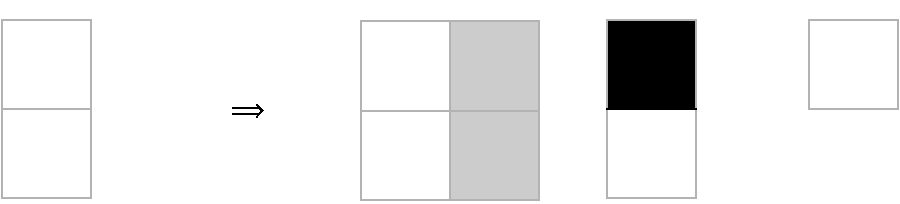
\includegraphics[ width = 4in ]{pdf/more_examples/svd_02_01_01} 
%  ` \caption{example caption}
   \label{fig:examples:21}
\end{figure}

The $\X{}$ matrix is trivial. Since it must be unitary the magnitude is one:
\begin{equation}
  \X{}= \mat{c}{1}.
\end{equation}
The lone singular value is the scale factor $r=\sqrt{2^{2}+\frac{1}{2}^{2}}$ which is the length of the vector:
\begin{equation}
  \sig{} = \mat{c}{\frac{\sqrt{5}}{2}\\0}.
\end{equation}
  For the codomain matrix we start with the image and normalize the column vector:
\begin{equation}
  \Y{}=\mat{cc}{c_{1}&c_{2}}, \qquad c_{1}=\frac{\sqrt{5}}{2}\mat{c}{2\\1}.
\end{equation}
The only quantity missing now is the null space vector $c_{2}$. Pick an orthogonal complement to $c_{1}$ and the codomain basis matrix is
\begin{equation}
  \Y{}=\frac{1}{\sqrt{5}}\mat{rr}{2&1\\1&-2}.
\end{equation}
The \svdl \ is then
\begin{equation}
  \begin{split}
    \svda{T}\\
    \mat{c}{1\\\frac{1}{2}} &= \frac{1}{\sqrt{5}}
    \mat{rr}{2&-1\\1&2}
    \mat{c}{\frac{\sqrt{5}}{2}\\0}
    \mat{c}{1}.
  \end{split}
  \label{eq:cases:2vdecomp}
\end{equation}

%%
\subsection{\vvv s}
Consider this \vvv:
\begin{equation}
  v = \mat{r}{1\\2\\-2}.
\end{equation}
The decomposition will have the shapes given by this
\begin{equation}
  \begin{array}{ccccc}
  \A{} &=& \Y{} & \sig{} & \X{T}\\
  \by{m}{n}&=&\paren{\by{m}{m}}&\paren{\by{m}{n}}&\paren{\by{n}{n}}\\
  \by{3}{1}&=&\paren{\by{3}{1}}&\paren{\by{3}{1}}&\paren{\by{1}{1}},
  \end{array}
\end{equation}
as shown here:
\begin{figure}[htbp] %  figure placement: here, top, bottom, or page
   \centering
   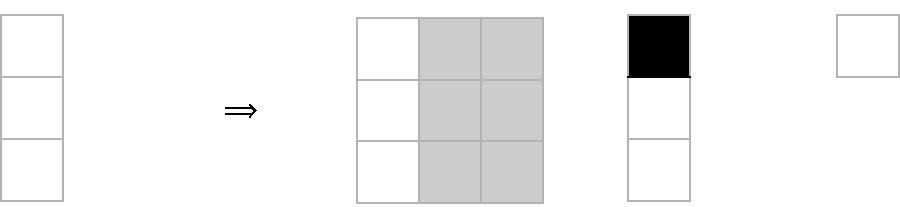
\includegraphics[ width = 4in ]{pdf/more_examples/svd_03_01_01} 
%   \caption{example caption}
   \label{fig:examples:31}
\end{figure}

We can use this vector to seed the codomain matrix:
\begin{equation}
  \Y{}_{*,1} = \frac{1}{3}\mat{r}{1\\2\\-2}.
\end{equation}
This leaves the null space vectors. A first candidate is 
\begin{equation}
  \Y{}_{*,2} = \frac{1}{\sqrt{2}}\mat{r}{0\\1\\1}.
\end{equation}
Using an inspection-based algorithm we can pick a vector like
\begin{equation}
  \Y{}_{*,3} = \frac{1}{\sqrt{18}}\mat{r}{4\\-1\\1}.
\end{equation}
The lone singular value is the length of the vector. The \svdl \ becomes
\begin{equation}
  \begin{split}
    \svda{T}\\
    \mat{r}{1\\2\\-2} &=
    \left[
\begin{array}{ r >{\columncolor{ltgray}}r >{\columncolor{ltgray}}r }
  \frac{1}{3} & 0 & \frac{4}{ \sqrt{18} } \\[5pt]
  \frac{2}{3} & \frac{1}{\sqrt{2}} & -\frac{1}{ \sqrt{18} } \\[5pt]
 -\frac{2}{3} & \frac{1}{\sqrt{2}} &  \frac{1}{ \sqrt{18} }
\end{array}
\right] 
    \left[
\begin{array}{c}
 3 \\ \hline
 0 \\
 0
\end{array}
\right]
  \mat{c}{1}.
  \end{split}
\end{equation}

The shortcut won't work. 
\begin{equation}
  v = \mat{c}{\sin\theta \\ 0 \\ \cos\theta}.
\end{equation}

\begin{equation}
  \begin{split}
    \W{y} = v v^{\mathrm{T}} &= \mat{c}{\sin\theta \\ 0 \\ \cos\theta}\mat{ccc}{\sin\theta & 0 & \cos\theta}\\
    &= \mat{ccc}{\sin^{2}\theta & 0 & \sin\theta \cos\theta\\ 0 & 0 & 0 \\ \sin\theta \cos\theta & 0 & \cos^{2}\theta}
  \end{split}
\end{equation}


Characteristic polynomial
Use cofactor expansion to compute the determinant
\begin{equation}
  \begin{split}
    p(\lambda) &= \det \paren{\W{y} - \lambda \I{3}}\\ &= 
    \det\mat{c|r|c}{\sin^{2}\theta - \lambda & 0 & \sin\theta \cos\theta\\\hline 0 & - \lambda & 0 \\ \sin\theta \cos\theta & 0 & \cos^{2}\theta- \lambda} \\
    &= \paren{\sin^{2}\theta - \lambda}\det\mat{cc}{-\lambda & 0 \\ 0 & \cos^{2}\theta- \lambda}\\ & \quad- 0 \det\mat{cc}{0 & 0 \\ \sin\theta \cos\theta & \cos^{2}\theta- \lambda}\\
     & \quad + \paren{\cos^{2}\theta - \lambda}\det\mat{cc}{0 & -\lambda \\ \sin\theta \cos\theta & 0}\\
  \end{split}
\end{equation}

The roots of the characteristic polynomial are the eigenvalues
\begin{equation}
  p(\lambda) = \lambda^{2}\paren{\lambda-1} = 0
\end{equation}
leads to the spectrum
\begin{equation}
  \lambda\paren{\W{y}} = \lst{1,0,0}.
\end{equation}
Therefore there is one singular value, 
\begin{equation}
  \sigma_{1} = 1.
\end{equation}
The eigenvector solves
\begin{equation}
  \begin{split}
    \W{y}u &= \lambda u\\
    \mat{ccc}{\sin^{2}\theta & 0 & \sin\theta \cos\theta\\ 0 & 0 & 0 \\ \sin\theta \cos\theta & 0 & \cos^{2}\theta} \mat{c}{u_{1} \\ 0 \\ u_{3}} & = \mat{c}{u_{1} \\ 0 \\ u_{3}}
  \end{split}
\end{equation}
This reduces to the system
\begin{equation}
\mat{cc}
{\sin^{2}\theta & \sin\theta \cos\theta\\
 \sin\theta \cos\theta & \cos^{2}\theta}
\mat{c}{u_{1} \\ u_{3}} = \mat{c}{u_{1} \\ u_{3}}
\end{equation}



%%
\subsection{$10-$vectors}
You can quickly verify that
\begin{equation}
  \begin{split}
    \svda{T}\\
    \mat{r}{1\\0\\0\\0\\0\\0\\0\\0\\0\\0} &=
    \left[
\begin{array}{ r >{\columncolor{ltgray}}r >{\columncolor{ltgray}}r >{\columncolor{ltgray}}r >{\columncolor{ltgray}}r >{\columncolor{ltgray}}r >{\columncolor{ltgray}}r >{\columncolor{ltgray}}r >{\columncolor{ltgray}}r >{\columncolor{ltgray}}r }
  1 & 0 & 0 & 0 & 0 & 0 & 0 & 0 & 0 & 0 \\
  0 & 1 & 0 & 0 & 0 & 0 & 0 & 0 & 0 & 0 \\
  0 & 0 & 1 & 0 & 0 & 0 & 0 & 0 & 0 & 0 \\
  0 & 0 & 0 & 1 & 0 & 0 & 0 & 0 & 0 & 0 \\
  0 & 0 & 0 & 0 & 1 & 0 & 0 & 0 & 0 & 0 \\
  0 & 0 & 0 & 0 & 0 & 1 & 0 & 0 & 0 & 0 \\
  0 & 0 & 0 & 0 & 0 & 0 & 1 & 0 & 0 & 0 \\
  0 & 0 & 0 & 0 & 0 & 0 & 0 & 1 & 0 & 0 \\
  0 & 0 & 0 & 0 & 0 & 0 & 0 & 0 & 1 & 0 \\
  0 & 0 & 0 & 0 & 0 & 0 & 0 & 0 & 0 & 1 \\
\end{array}
\right] 
    \left[
\begin{array}{c}
 1 \\ \hline
 0 \\
 0 \\
 0 \\
 0 \\
 0 \\
 0 \\
 0 \\
 0 \\
 0
\end{array}
\right]
  \mat{c}{1}.
  \end{split}
\end{equation}

This is such a simple exercise because the column vectors are already unit vectors.

A Givens rotation by an angle $\theta$ in the $4-8$ plane does not affect the decomposition because the codomain matrix $\Y{}$ is still orthogonal
\begin{equation}
  \Y{'} = 
      \left[
\begin{array}{ c >{\columncolor{ltgray}}c >{\columncolor{ltgray}}c >{\columncolor{ltgray}}c >{\columncolor{ltgray}}c >{\columncolor{ltgray}}c >{\columncolor{ltgray}}c >{\columncolor{ltgray}}c >{\columncolor{ltgray}}c >{\columncolor{ltgray}}c }
  1 & 0 & 0 & 0 & 0 & 0 & 0 & 0 & 0 & 0 \\
  0 & 1 & 0 & 0 & 0 & 0 & 0 & 0 & 0 & 0 \\
  0 & 0 & 1 & 0 & 0 & 0 & 0 & 0 & 0 & 0 \\
  0 & 0 & 0 & \cos \theta & 0 & 0 & 0 & -\sin \theta & 0 & 0 \\
  0 & 0 & 0 & 0 & 1 & 0 & 0 & 0 & 0 & 0 \\
  0 & 0 & 0 & 0 & 0 & 1 & 0 & 0 & 0 & 0 \\
  0 & 0 & 0 & 0 & 0 & 0 & 1 & 0 & 0 & 0 \\
  0 & 0 & 0 & \sin \theta & 0 & 0 & 0 & \cos \theta & 0 & 0 \\
  0 & 0 & 0 & 0 & 0 & 0 & 0 & 0 & 1 & 0 \\
  0 & 0 & 0 & 0 & 0 & 0 & 0 & 0 & 0 & 1 \\
\end{array}
\right] 
\end{equation}

Yet another rotation 1-9:
\begin{equation}
  \Y{'} = 
      \left[
\begin{array}{ c >{\columncolor{ltgray}}c >{\columncolor{ltgray}}c >{\columncolor{ltgray}}c >{\columncolor{ltgray}}c >{\columncolor{ltgray}}c >{\columncolor{ltgray}}c >{\columncolor{ltgray}}c >{\columncolor{ltgray}}c >{\columncolor{ltgray}}c }
  \cos \phi & 0 & 0 & 0 & 0 & 0 & 0 & 0 & -\sin \phi & 0 \\
  0 & 1 & 0 & 0 & 0 & 0 & 0 & 0 & 0 & 0 \\
  0 & 0 & 1 & 0 & 0 & 0 & 0 & 0 & 0 & 0 \\
  0 & 0 & 0 & \cos \theta & 0 & 0 & 0 & -\sin \theta & 0 & 0 \\
  0 & 0 & 0 & 0 & 1 & 0 & 0 & 0 & 0 & 0 \\
  0 & 0 & 0 & 0 & 0 & 1 & 0 & 0 & 0 & 0 \\
  0 & 0 & 0 & 0 & 0 & 0 & 1 & 0 & 0 & 0 \\
  0 & 0 & 0 & \sin \theta & 0 & 0 & 0 & \cos \theta & 0 & 0 \\
  \sin \phi & 0 & 0 & 0 & 0 & 0 & 0 & 0 & \cos \phi & 0 \\
  0 & 0 & 0 & 0 & 0 & 0 & 0 & 0 & 0 & 1 \\
\end{array}
\right] 
\end{equation}


\endinput
\section{Matrices}
For clarity matrices are typeset in emboldened letters. Throughout this book we will be considering matrices in general as a collection of complex numbers with $m$ rows and $n$ columns. The height of the matrix is determined by $m$, the number of rows; the width by $n$ the number of columns. The important point is that the number of rows are specified first, then the number of columns:
\begin{equation}
  \paren{\by{rows}{columns}}=\paren{\by{m}{n}}.
\end{equation}
The first row is the top row and the first column is the left-most column.

Formally we specify a matrix as
\begin{equation}
  \A{}\in\cmplx{\by{m}{n}}
\end{equation}
even if only one entry is complex. If all matrix entries are real we instead write
\begin{equation}
  \A{}\in\real{\by{m}{n}}.
\end{equation}
It is not so much the collection of numbers that is of interest here as the meaning of the rows and columns. But other properties require explanation first.

%%
\subsection{Matrix rank}
A critical matrix property is rank\index{rank!matrix}, denoted here by the parameter $\rho$.  The rank details the number of independent rows or columns. You may speak of row rank\index{rank!row}, the number of independent rows, or column rank\index{rank!column}, the number of independent columns. However the matrix rank is the same as the row rank and the same as the column rank. 
$$
\text{matrix rank} = \text{row rank} = \text{column rank}.
$$
Below are some examples of $\bys{3}$ matrices of different ranks in reduced form.
\begin{equation}
\begin{array}{ccc}
\mat{rcr}
{
-2 & e^{-1} & 1\\
 0 &  i & 0\\
 0 &  0 &-4
}, \qquad & 
\mat{ccc}
{
 1 &  2i & 0\\
 0 &  8 & \pi\\
 0 &  0 & 0
}, \qquad & 
\mat{rrc}
{
\sqrt[4]{2} & -1 & \pi^{2}\\
 0 &  0 & 0\\
 0 &  0 & 0
} \\[5pt]
\rho = 3 & \rho = 2 & \rho = 1
\end{array}
\end{equation}

Certainly then the rank can be no larger than the minimum of the dimension parameters $m$ and $n$. That is
\begin{equation}
  \rho \le \min \lst{m,n}.
\end{equation}
To include the rank in the matrix specification use a subscript as shown here
\begin{equation}
  \A{}\in\cmplx{\by{m}{n}}_{\rho}.
\end{equation}

For example, consider a matrix with three rows, but only two are linearly independent. The second row is equal to two times the first row minus the third row. This matrix is
\begin{equation}
  \A{}\in\cmplx{\by{3}{columns}}_{2} = \mat{c}
  {
  r_{1}\\ \hline
  2r_{1}-r_{3}\\ \hline
  r_{3}
  }.
\end{equation}
Because there are two linearly independent rows, row 1 and row 3, the row rank of this matrix is $\rho = 2$. Therefore the matrix rank is also two. Notice that the number of columns must be $n \ge \rho$. 

The same principle applies to the columns. Here is a matrix where the first column is the sum of last three columns. This matrix is
\begin{equation}
  \A{}\in\cmplx{\by{rows}{4}}_{3} = \mat{c|c|c|c}
  {
  c_{2}+c_{3}-c_{4} & c_{2} & c_{3} & c_{4}
  }.
\end{equation}
Because there are three linearly independent columns, rows 2, 3, and 4, the column rank of this matrix is $\rho = 3$. Therefore the matrix rank is also three. The number of rows must be $m \ge \rho$.

The matrices generated by the outer product are all rank one matrices as shown by equation \eqref{prelim:vectors:outer}. Each row is a multiple of the input row vector.

The concept of matrix rank is a rich one which will prove invaluable. Further explanation is deferred.

%%
\subsection{Matrix multiplication}
There are a few ways to address matrix multiplication\index{matrix!multiplication}. The paradigm of interest here is to cast matrix multiplication as a series of dot products between row vectors and column vectors. For the matrix equation
\begin{equation}
  \begin{array}{cccc}
  \A{}&\B{} &=& \C{}\\
  \paren{\by{m}{p}} & \paren{\by{p}{n}} && \paren{\by{m}{n}}
  \end{array}
  \label{eq:mprod}
\end{equation}
the element of the product matrix $\C{}$ in row $r$ and column $c$ is given by the dot product of the $r$th row of $\A{}$ with the $c$th column of $\B{}$. The result is the scalar $\C{}_{r,c}$. This equation may simpler to understand than the words:
\begin{equation}
  \C{}_{r,c} = \underbrace{\A{}_{r,*}}_{\text{row }r}\cdot\underbrace{\B{}_{*,c}}_{\text{col }c}.
  \label{eq:dot}
\end{equation}
An schematic example is shown in figure \eqref{fig:1:mmult} where $\C{}_{2,4} = \A{}_{2,*}\cdot\B{}_{*,4}.$
%%%
\begin{figure}[htbp] %  figure placement: here, top, bottom, or page
   \centering
   \includegraphics[]{pdf/prelim/multiply.pdf} 
   \caption[Each entry in a product matrix is computed as a dot product]{Each entry in a product matrix is computed as a dot product. Row vectors on the left matrix are dotted with column vectors in the right matrix. The concept of conformability for $\A{}\B{}=\C{}$ is distinctly shown here as both vectors must have the same length.}
   \label{fig:1:mmult}
\end{figure}
%%%
The dot product rule dictates the conformability condition\index{conformability condition}. For a product matrix of dimension $\by{m}{n}$ the component matrices must have the dimensions
of $\by{m}{p}$ for the left matrix and $\by{p}{n}$ for the right matrix as shown in equation \eqref{eq:mprod} and emphasized here
\begin{equation}
\paren{\by{m}{p}}\paren{\by{p}{n}}=\by{m}{n}.
\end{equation}
The crucial observation is that the vectors in the dot product have common dimension $p$.

Because it is easy to confuse the convention\footnote{Meyer has a very nice explanation of the source of the convention in his book, \cite[p. 123]{Meyer}.} an example follows. Think of an example of two matrices multiplied in different orders. Take a wide matrix that is $m \times n = 2\times5$ and a tall matrix that is $5\times 2$. Multiply wide by tall, then tall by wide and look at the shape of the product matrices. This realization will be recalled in the section on product matrices,
%%%
\begin{figure}[htbp] %  figure placement: here, top, bottom, or page
\includegraphics[ width = 3.75in ]{pdf/prelim/mult_prods}\\
   \caption[Shape dynamics]{Shape dynamics. The product matrix inherits the height from the matrix on the left, the width from the matrix on the right. That is height from the left, width from the right.}
   \label{fig:example}
\end{figure}
%%%
%%
\subsection{The matrix transpose}
The matrix transpose appears over and over throughout linear algebra and is a generalization of vector transposition.

Taking the transpose of a matrix means interchanging the rows and columns. Row 1 becomes column 1, row 2 becomes column 2, and so on. The rule has the result
\begin{equation}
  \begin{split}
    \A{}&\in\cmplx{\by{m}{n}},\\
    \A{T}&\in\cmplx{\by{n}{m}},
  \end{split}
\end{equation}
showing the interchange of $m$ and $n$.

If $\A{}$ had $m=5$ rows and $n=2$ columns the transpose $\A{T}$ will have $m=2$ rows and $n=5$ columns. 
Taking the transpose of the transpose restores the target matrix to original form. That is,
\begin{equation}
  \paren{\A{T}}^{\mathrm{T}}=\A{}.
\end{equation}

An elementary exercise, e.q. \cite[p. 10]{Meyer}, \cite[p. 8]{Strang}, shows the reverse order rule for matrix products:
\begin{equation}
  \paren{\A{}\B{}}^{\mathrm{T}}=\B{T}\A{T}.
  \label{eq:mattran}
\end{equation}

Philosophically, neither matrix nor transpose is a more fundamental object than the other. Certainly in terms of a specific computation there will be a preference flowing from the association with the rows and columns. But without an association to a measurement system, a matrix and its transpose share equivalence. Ultimately this lack of ascendancy will lead to the concept of domain and codomain.

%%
\subsection[Matrices do not commute]{Matrices do not commute under multiplication}
Matrices share many properties with scalars like associativity and distributivity. But matrices do not commute in general. That is typically
\begin{equation}
  \brac{\A{},\B{}} = \A{}\B{}-\B{}\A{} \ne \zero.
  \label{eq:matcom}
\end{equation}

A quick way to realize this is to imagine a rectangular matrix where $m\ne n$. The product matrix $\A{}\A{T}$ is a square matrix of dimensions $\by{m}{m}$ and the product matrix $\A{T}\A{}$ is a square matrix of dimensions $\by{n}{n}$. We cannot difference these matrices of different sizes.

What if the problem is restricted to the class of square matrices where $m=n$? Then the issue is that we are using \textit{different vectors} in the dot products. Rewrite \eqref{eq:matcom} as 
\begin{equation}
  \brac{\A{},\B{}} = \A{}\B{}-\B{}\A{} = \overrightarrow{\C{}} - \overleftarrow{\C{}}
\end{equation}
and consider the matrix elements 
\begin{equation}
  \begin{split}
    \overrightarrow{\C{}}_{r,c} &= \A{}_{r,*}\cdot\B{}_{*,c},\\
    \overleftarrow{\C{}}_{r,c} &= \B{}_{r,*}\cdot\A{}_{*,c}.\\
  \end{split}
\end{equation}
In general
\begin{equation}
   \overrightarrow{\C{}}_{r,c} \ne \overleftarrow{\C{}}_{r,c}
\end{equation}
because
\begin{equation}
  \A{}_{r,*}\cdot\B{}_{*,c} \ne \B{}_{r,*}\cdot\A{}_{*,c}.
\end{equation}
The issue is that in one direction, $\A{}\B{}$, we are using the \textit{row} vectors of $\A{}$. The other direction, $\B{}\A{}$, involves the \textit{column} vectors of $\A{}$. Clearly, the general matrix does not enforce an equality between row and column vectors.

%%
\subsection{The adjoint}
One of the most important operations we will perform on a matrix is the \textit{adjoint}\index{adjoint} operation, also called \index{Hermitian conjugation}\textit{Hermitian conjugation.} This interchanges the rows and columns and requires that we take the complex conjugate of each matrix entry. If $a_{r,c}$ is the element in row $r$ and column $c$ the matrix $\A{}$ then we can symbolically represent this process as 
\begin{equation}
  \begin{split}
    \A{} &\to \A{*}\\
    a_{r,c} &\to \overline{a}_{c,r}
  \end{split}
\end{equation}

The complex conjugate of this element will appear in row $c$ and column $r$ in the matrix $\A{*}$.

When working with complex matrices
\begin{equation}
    \A{*}= \overline{\A{}}^{\mathrm{T}}= \overline{\A{T}}.
\end{equation}
The operations of conjugation and transposition commute; that is, they can be performed in any order as shown above.

Quite often we will restrict our attention to the field of real numbers and dispense with the generality of the complex field. In these cases the adjoint is the transpose.

%%
\subsection{Product matrices}
Product matrices are an important topic for this book. In general the matrices that we study are not square which makes it impossible to discuss important properties like eigenvalues. To extend these concepts to rectangular matrices, form either of the square matrices
\begin{equation}
  \begin{split}
    \W{x} &= \prdm{*}, \\
    \W{y} &= \prdmm{*}.
    \label{eq:prelim:w}
  \end{split}
\end{equation}
The astute reader may wonder about the assignment of the subscripts for the product matrices. The convention is rudimentary:
\begin{enumerate}
\item $\W{x}\in\cmplx{\by{n}{n}}$ and is conformable with $n-$vectors from the \textit{domain};
\item $\W{y}\in\cmplx{\by{m}{m}}$ and is conformable with $m-$vectors from the \textit{codomain}.
\end{enumerate}
This foreshadows the richer context of matrix domain.

While the term ``product matrix'' has the general connotation as in equation \eqref{eq:mprod}, in this work ``product matrices'' implies $\W{x}$ and $\W{y}$, the two situations where a matrix is multiplied with its adjoint.

%%
\subsection{Left and right operations}
A recurring theme in this book are left and right operations on matrices. 
The usual condition is when the target matrix premultiplies a vector as in 
\begin{equation}
\A{}x=y.
\label{eq:axy}
\end{equation}
Another option is postmultiplication of the vector by the matrix. This can be expressed by premultiplication of the transpose matrix upon the vector transpose:
\begin{equation}
  \paren{y^{\mathrm{T}}\A{}}^{\mathrm{T}} = \A{T}y=x.
\label{eq:ayx}
\end{equation}
These last two statements have deep implications. We see that the target matrix operates on an $n-$vector $x$ and returns an $m-$vector $y$. Also, the transpose matrix operates on an $m-$vector $y$ and returns an $n-$vector $x$. (Please be very clear that the vector pairs $(x,y)$ in \eqref{eq:axy} are different from the vector pairs $(x,y)$ in \eqref{eq:ayx}. The transpose is not an inverse; the transpose always exists, the inverse sometimes so.)

We saw that matrices operate upon column vectors on the right and that row vectors on the left operate upon matrices.

When we examine the pseudoinverse, the generalized matrix inverse, we will that every matrix $\A{}$ has a pseudoinverse $\A{+}$. In some cases this will be a left inverse
\begin{equation}
  \leftinv = \I{n},
\end{equation}
in other cases it may be a right inverse
\begin{equation}
  \rightinv = \I{m}.
\end{equation}
In the first case premultiplication by the pseudoinverse produced an identity matrix. In the second case postmultiplication produced an identity matrix.

%%
\subsection{Domain and codomain}
A matrix is a map between two vector spaces, the space of $m-$vectors and the space of $n-$vectors. So both spaces are domains. By convention the space of $n-$vectors is called the \index{domain and codomain}\textit{domain} and the space of $m-$vectors is called the \index{codomain}\textit{codomain}. Therefore neither domain nor codomain is a more fundamental object.

Going back we can read this equation
\begin{equation*}
  \A{}x=y
\end{equation*}
as ``The matrix $\A{}$ maps $n-$vectors in the domain $X$ to $m-$vectors in the codomain $Y$.''
We can read the equation
\begin{equation*}
  \A{*}y=x
\end{equation*}
as ``The adjoint matrix $\A{*}$ maps $m-$vectors in the codomain $Y$ to $n-$vectors in the domain $X$.''

More formally, the vector space $X$ is the set of all vectors of length $n$. Of course then the vector space $Y$ is the set of all vectors of length $m$.

To close this section we present a summary table.
%%%
\begin{table}[htdp]
\begin{center}
\begin{tabular}{llcl}
  matrix & maps from  && maps to \\\hline
  $\A{}$ & domain   & $\mapsto$ & codomain \\
         & \mv s    & $\mapsto$ & \nv s \\
         & $X$      & $\mapsto$ & $Y$    \\[3pt]
  $\A{*}$& codomain & $\mapsto$ & domain \\
         & \nv s    & $\mapsto$ & \mv s \\
         & $Y$      & $\mapsto$ & $X$    
\end{tabular}
\end{center}
\label{tab:00:mappings}
\caption{Matrix mapping actions. Here $\Accmn$ and we see how the matrix and it adjoint maps between the domain and the codomain.}
\end{table}%


%%
\subsection{The range of a matrix}
A bedrock concept of linear algebra is the \textit{range}\index{range} of a matrix. The range of a matrix $\A{}$ is the collection of all possible $m-$vectors generated by the matrix $\A{}$ when acting upon $n-$vectors:
\begin{equation}
  \rng{\A{}}=\lst{\A{}x\colon x \in \cmplx{n}}\subseteq \cmplx{m}.
\end{equation}

For example the range of the identity matrix
\begin{equation}
  \I{2}=\mat{cc}{1&0\\0&1}
\end{equation}
is the entire plane $\real{2}$. Any point in the plane can be reached with the appropriate $x$ vector. The arbitrary point 
\begin{equation}
  p = \mat{c}{\alpha \\ \beta}
\end{equation}
can be reached by using the vector
\begin{equation}
  x = \mat{c}{\alpha \\ \beta}
\end{equation}
since 
\begin{equation}
  \A{} x = p.
\end{equation}

However for matrices that do not have full rank there will always be restrictions on the range. It will not be $\real{m}$. The matrix
\begin{equation}
  \A{}=\mat{cc}{1&0\\0&0}
\end{equation}
can only produce vectors on the $x-$axis. There are no vectors which map to the any point with a non-zero $y-$coordinate. For example, there exists no such vector $x$ which solves 
\begin{equation}
  \A{}x=\mat{cc}{1&0\\0&0}\mat{c}{x_{1}\\x_{2}} = \mat{c}{0\\1}.
\end{equation}

The geometric interpretation of range\index{range!geometric interpretation} leads to the a different perspective of matrix actions upon vectors. When a matrix acts upon a vector the result is a linear combination of the column vectors of the matrix as shown below:
\begin{equation}
\begin{split}
  \A{}x&=\mat{c|c|c|c}{\A{}_{*,1} & \A{}_{*,2} & \A{}_{*,3} & \hdots}\mat{c}{x_{1} \\ x_{2} \\ x_{3} \\ \vdots} \\
    &= x_{1} \A{}_{*,1} + x_{2} \A{}_{*,2} + x_{3} \A{}_{*,3} + \dots .
\end{split}
\end{equation}
In this context, the range of a matrix is all possible linear combinations of the column vectors. Since this concept can also be framed as all possible combinations of the column vectors, the range is sometimes called the image space\index{image space} (or image) of a matrix.

%%
\subsection{The condition number}
The condition number, $\kappa$, is one of the most important diagnostic quantities we have for a matrix. It is a measure of the precision of the inverse mapping. A simple example illustrates the point. Examine the matrix sequence
\begin{equation}
\begin{array}{ccccc}
  \mat{cc}{1&0\\0&1} & \to & \mat{cc}{1&0\\0&\epsilon} & \to & \mat{cc}{1&0\\0&0}\\[15pt]
  \kappa = 1 && \kappa = 1/\epsilon && \kappa = \infty.
\end{array}
\end{equation}
The matrix on the left, the identity matrix has the ideal condition number of unity. The matrix on the right is rank-deficient and has infinite condition number. The matrix in the middle has ambiguous condition number and we see that as the parameter $\epsilon$ varies from 1 to 0 the conditioning goes from ideal to disasterous. In fact, one would certainly suspect that as $\epsilon$ nears the machine epsilon of your computer computations involving this matrix will be unreliable.

A more formal definition will follow later because the emphasis here is on intuition. For now consider three basic cases:
\begin{enumerate}
\item The ideal case, $\kappa=1$, for exact maps like identity matrices. This means that all vectors $\paren{y_{1},y_{2}}^{\mathrm{T}}$ in the codomain  can be exactly mapped to all source vectors $\paren{x_{1},x_{2}}^{\mathrm{T}}$ in the domain by the matrix inverse.
\item Imprecise maps where the condition number is large. Some vectors $\paren{y_{1},y_{2}}^{\mathrm{T}}$ in the codomain may be mapped by the inverse not to the source vector $\paren{x_{1},x_{2}}^{\mathrm{T}}$, but instead to a nearby vector.
\item Frustrated maps where $\kappa=\infty$. Entire classes of vectors $\paren{y_{1},y_{2}}^{\mathrm{T}}$ in the codomain cannot be mapped to any vectors in the domain $\paren{x_{1},x_{2}}^{\mathrm{T}}$.
\end{enumerate}

%%
\subsection{A note on terminology}
Basic terminology differences distinguish between real and complex matrices. If all entries in a matrix are real, then the matrix is real. If at least one matrix entry is imaginary or complex, then the matrix is complex. Many texts avoid stirring complex numbers into the mix. The philosophy here is that the added intricacy of complex arithmetic is more than offset by the unique properties we will explore in the complex realm.

The table below shows the differences in terminology between real and complex matrices.
\begin{equation}
\boxed{
\begin{array}{cc}
  \text{real matrices} & \text{complex matrices} \\\hline\hline
  \text{transpose} & \text{adjoint} \\
  \A{T} & \A{*} \  \paren{= \overline{\A{T}}} \\[10pt]\hline
  \text{orthogonal} & \text{unitary} \\
  \A{-1}=\A{T} & \A{-1}=\A{*}
\end{array}
}
\end{equation}

The complex notation is more general and should be used if the matrix entries are not restricted to be real numbers. However if all matrix entries are real the custom is to use notation for real matrices. 

\endinput
% bys
\newcommand{\by}[2]      {#1 \times #2}
\newcommand{\byy}[1]     {#1 \times #1}
\newcommand{\bymn}[0]    {\by{m}{n}}
\newcommand{\bymm}[0]    {\byy{m}}
\newcommand{\bynn}[0]    {\byy{n}}
\newcommand{\bynm}[0]    {\by{n}{m}}
\newcommand{\bymr}[0]    {\by{m}{\rho}}
\newcommand{\byrn}[0]    {\by{\rho}{n}}

% vector spaces
\newcommand{\real}[1]    {\mathbb{R}^{#1}}
\newcommand{\cmplx}[1]   {\mathbb{C}^{#1}}
\newcommand{\either}[1]  {\cmplx{#1}}
\newcommand{\ir}[0]      {\in\real{}}
\newcommand{\ic}[0]      {\in\cmplx{}}
\newcommand{\icm}[0]     {\in\cmplxm}
\newcommand{\icn}[0]     {\in\cmplxn}
\newcommand{\icmn}[0]    {\in\cmplxmn}
\newcommand{\irmn}[0]    {\in\realmn}
\newcommand{\icmnr}[0]   {\in\cmplxmnr}
\newcommand{\ints}[0]    {\mathbb{Z}}
\newcommand{\natnum}[0]  {\mathbb{N}}

\newcommand{\iints}[0]   {\in \mathbb{Z}}
\newcommand{\inatnum}[0] {\in \mathbb{N}}

\newcommand{\realall}[3] {\real{\by{#1}{#2}}_{#3} }
\newcommand{\cmplxall}[3]{\cmplx{\by{#1}{#2}}_{#3} }

\newcommand{\realn}[0]   {\real{n}}
\newcommand{\realm}[0]   {\real{m}}
\newcommand{\realmn}[0]  {\real{\bymn}}
\newcommand{\realnn}[0]  {\real{\byy{n}}}
\newcommand{\realmm}[0]  {\real{\byy{m}}}
\newcommand{\realmmr}[0] {\real{\byy{m}}_{\rho}}
\newcommand{\realmmm}[0] {\realmm_{m}}

\newcommand{\cmplxn}[0]  {\cmplx{n}}
\newcommand{\cmplxm}[0]  {\cmplx{m}}
\newcommand{\cmplxnn}[0] {\cmplx{\byy{n}}}
\newcommand{\cmplxmm}[0] {\cmplx{\byy{m}}}
\newcommand{\cmplxmn}[0] {\cmplx{\bymn}}
\newcommand{\cmplxmr}[0] {\cmplx{\bymr}}
\newcommand{\cmplxrn}[0] {\cmplx{\byrn}}
\newcommand{\cmplxmnr}[0]{\cmplx{\bymn}_{\rho}}
\newcommand{\cmplxmmm}[0]{\cmplxmm_{m}}
\newcommand{\cmplxmnm}[0]{\cmplxmn_{m}}
\newcommand{\cmplxnnr}[0]{\cmplxnn_{\rho}}
\newcommand{\cmplxmnn}[0]{\cmplxmn_{n}}

% spans
\newcommand{\spn}[1]     {\text{sp\,} \lst{ #1 }}


\endinput  %  -  -  -  -  -  -  -  -  -  -  -  -  -  -  -  -  -  -  -  -
\section{More on domains}
A considerable portion of the theoretical discussions to follow is based upon a clear understanding of domains and complete spaces. 

%%
\subsection{The mapping action of the matrix $\A{}$}
Pick an example matrix 
\begin{equation}
  \A{}\in\cmplx{\by{3}{2}}.
\end{equation}
This matrix maps \vv s to \vvv s. We will represent the collection of all \vv s as a square on the left and the collection of all \vvv s as a square on the right. The target matrix $\A{}$ connects points in the left square with points in the right square as shown in figure \eqref{fig:mapa}:

\begin{figure}[htbp] %  figure placement: here, top, bottom, or page
   \centering
   \includegraphics[ ]{pdf/prelim/map_01} 
   \caption{Generic mapping actions. The domain $\X{}$ is the collection of \vv s; the codomain $\Y{}$ is the collection of \vvv s. The matrix $\A{}$ connects each \vv \ to a \vvv.}
   \label{fig:mapa}
\end{figure}

Or symbolically
\begin{equation}
  \A{} \mat{c}{\star \\ \star} = \mat{c}{\bullet \\ \bullet \\ \bullet }.
\end{equation}

%%
\subsubsection{Going from domain to codomain}
The cases of interest are when then map is frustrated and unable to reach the entire codomain. For example, the matrix 
\begin{equation}
  \A{}= \Aexample
  \label{eq:A}
\end{equation}
maps \vv s to \vvv s. The problem is that this matrix cannot connect to the entire set of \vvv s. In fact, this matrix can only see a limited set of \vvv s. To understand why, look at the general problem
\begin{equation}
  \A{} x = \Aexample \mat{c}{x_{1}\\x_{2}} = \alpha\mat{r}{1\\-1\\1}
\end{equation}
where $\alpha = x_{1}-x_{2}$. The three vector describe the line through origin and the point $p=\mat{ccc}{1&-1&1}$. The position on this line is completely encoded in the parameter $\alpha$.

For example, there is no vector in the domain which maps to the constant vectors:
\begin{equation}
  \Aexample \mat{c}{x_{1}\\x_{2}} \ne \mat{c}{1\\1\\1}.
\end{equation}
Let's revise the diagram to show that the map is frustrated and able to reach only some of the vectors in the codomain. The square representing the \vvv s will be separated into two regions. The shaded portion represents the \vvv s that can't be connected to any \vv \ under the mapping of $\A{}$. The result is figure \eqref{fig:map_01}.
\begin{figure}[htbp] %  figure placement: here, top, bottom, or page
   \centering
   \includegraphics[ ]{pdf/prelim/map_02} 
   \caption{The mapping action of the target matrix is frustrated and unable to reach most of the \vvv s in the codomain. The excluded portion of the codomain is represented by the shaded region on the right.}
   \label{fig:map_01}
\end{figure}

%%
\subsubsection{Going from codomain to domain}
Consider the action of the transpose: we start with a \vvv \  and map to a \vv. The transpose matrix is
\begin{equation}
  \A{T}= \Atexample.
\end{equation}
Here too there is a problem with the mapping and it cannot reach the full domain.
\begin{equation}
  \A{T} y = \Atexample \mat{c}{y_{1}\\y_{2}\\y_{3}} = \mat{r}{y_{1} - y_{2} + y_{3}\\-y_{1} + y_{2} - y_{3}} = \alpha\mat{r}{1\\-1}
\end{equation}
where this time $\alpha = y_{1}-y_{2}+y_{3}$. Notice for example there is no vector in the domain which maps to the constant vectors:
\begin{equation}
  \Atexample \mat{c}{y_{1}\\y_{2}\\y_{3}} \ne \mat{c}{1\\1}.
\end{equation}
The diagram for this process is shown in figure \eqref{fig:mapc}.
\begin{figure}[htbp] %  figure placement: here, top, bottom, or page
   \centering
   \includegraphics[ ]{pdf/prelim/map_04} 
   \caption{The mapping action of the transpose matrix is also frustrated and unable to reach most of the \vv s in the codomain. The excluded portion of the domain is represented by the shaded region on the left.}
   \label{fig:mapc}
\end{figure}

%%
\subsubsection{The round trip between codomain and domain}
With the separate actions of the target and transpose matrices resolved, the final diagram can be assembled. It is shown in figure \eqref{fig:mapd}.
\begin{figure}[htbp] %  figure placement: here, top, bottom, or page
   \centering
   \includegraphics[ ]{pdf/prelim/map_05} 
   \caption{The mapping actions of the matrix in equation \eqref{eq:A}. The matrix and its transpose map to a portion of $\cmplx{3}$ and a portion of $\cmplx{2}$ respectively.}
   \label{fig:mapd}
\end{figure}

%%
\subsubsection{Vector spaces}
The ultimate diagram in figure \eqref{fig:mapd} represents the mapping actions of the target and transpose matrices. The simplicity of the diagram robs us of an opportunity to quantify the issues with the mappings. Yet it provides a clear representation of the two maps within each matrix.

Figure \eqref{fig:mapd} is the mental picture that should form when you look at a matrix. This of course does not tell the complete story.

In the context of vector spaces we can make some powerful observations about the matrix $\A{}$. In both cases the spaces are incomplete. In the \vv \ case there is basically one vector, the first row:
\begin{equation}
  r_{1} = \mat{r}{1\\-1}.
\end{equation}
To complete the space $\real{2}$ we need another real vector. We choose an orthogonal\footnote{Orthogonality simplifies our manipulations.} vector
\begin{equation}
  r_{1}^{\perp} = \mat{r}{1\\1}.
\end{equation}
The symbol ``$\perp$'' means ``perpendicular to.'' That is
\begin{equation}
  r_{1}\cdot r_{1}^{\perp} = \mat{r}{1\\-1} \cdot \mat{c}{1\\1} = \mat{c}{0\\0} = \zero.
\end{equation}
With these two vectors we can span $\real{2}$, the plane. Mathematically the expression is this
\begin{equation}
  \real{2} = \spn \lst{r_{1},r_{1}^{\perp}} = \spn \lst{\mat{r}{1\\-1},\mat{c}{1\\1}}.
\end{equation}

To conceptualize the meaning of span, think of it as the collection of all vectors attained by scaling and combining the spanning vectors. In this case that would be
\begin{equation}
 \alpha\, r_{1} + \beta\, r_{1}^{\perp} = \alpha \mat{r}{1\\-1} + \beta \mat{c}{1\\1}
\end{equation}
where the scalars $\alpha, \beta$ are arbitrary.

Is this span a plane? Can we reach any arbitrary point in $\real{2}$ with this spanning set? Yes, for example
\begin{equation}
  \begin{split}
    \mat{c}{x\\y} &= \frac{1}{2}\paren{x-y}\mat{r}{1\\-1} + \frac{1}{2}\paren{x+y}\mat{r}{1\\1},\\
    &= \frac{1}{2}\mat{r|c}{1&1\\-1&1}\mat{c}{x+y\\x-y}.
  \end{split}
\end{equation}

The \vvv \ case is also begins with a lone vector, the first column:
\begin{equation}
  c_{1} = \mat{r}{1\\-1\\1}.
\end{equation}
To complete $\real{3}$ we need two vectors for an \index{orthogonal complement}orthogonal complement. One such choice is
\begin{equation}
  c_{1}^{\perp} = \spn \lst{\veca,\vecb},
\end{equation}
a plane.
Using the symbol $\oplus$ to denote the addition of vector spaces, the complete space becomes
\begin{equation}
  \real{3} = \spn \lst{\mat{r}{1\\-1\\1}} \oplus \spn \lst{\veca,\vecb}.
\end{equation}
Notice that the matrix only contained some of the information that we needed; \textit{the completion of the spaces was a separate process.}

Figure \eqref{fig:mape} shows the mapping process in diagram form against the resolution of the host spaces. The shaded regions represent the orthogonal complements to the row and column vectors in the matrix $\A{}$.
\begin{figure}[htbp] %  figure placement: here, top, bottom, or page
   \centering
   \includegraphics[ ]{pdf/prelim/map_06} 
   \caption{The mapping actions of the matrix $\A{}$ and the vector space decompositions. The shaded regions are the orthogonal complements spanned by the null space vectors.}
   \label{fig:mape}
\end{figure}

We are now at the point where we can close the discussion on domains. Many functions map from $\real{n}$ to $\real{m}$. Analogously, many matrices are complete maps from $\real{n}$ to $\real{m}$. There are classes of functions where the mapping is frustrated: either points in the domain $\real{n}$ are not accessible or points in the range $\real{m}$ are not accessible or both. 

In the matrix case these frustrated maps have special signatures. Consider the $3\times2$ matrix in equation \eqref{eq:A}. All $2-$vectors from $\real{n=2}$ are valid inputs, but it is not possible to map to all vectors in $\real{m=3}$. The matrix $\A{}$ maps the plane to a line, a line which lives in $\real{3}$.

Look at the figure \eqref{tab:0:rn} showing the hierarchy of domains. We can interpret it as showing the discrete steps of frustration. In the best case a $3\times2$ matrix will map from the plane $\real{2}$ to a volume $\real{3}$. If the map is frustrated, it will map from the plane $\real{2}$ to another plane. This plane is a two-dimensional object in three space. If the map has maximal frustration, as in equation \eqref{eq:0}, it will map from the plane $\real{2}$
to a line. This line is a one-dimensional object in three space.

For a matrix of size $m\times n$ the number of possible mappings is given by the parameter
\begin{equation}
  \nu = \min \lst{m, n}.
\end{equation}
Consider the set of arbitrary real $m\times n$ matrices. If the matrix is tall, then $m>n$ and it will have one and only one of these $n$ mapping actions:
\begin{equation}
\begin{array}{cccl}
\real{n} & \mapsto & \real{1} & \qquad \text{row rank deficiency} = n - 1,\\
\real{n} & \mapsto & \real{2} & \qquad \text{row rank deficiency} = n - 2,\\
& \vdots\\
\real{n} & \mapsto & \real{n} & \qquad \text{full row rank}.
\end{array}
\end{equation}
The frustrated mappings signal rank deficiencies.
If the matrix is wide, then $m<n$ and it will have one and only one of these $m$ mapping actions:
\begin{equation}
\begin{array}{cccl}
\real{n} & \mapsto & \real{1} & \qquad \text{row rank deficiency} = n - 1,\\
\real{n} & \mapsto & \real{2} & \qquad \text{row rank deficiency} = n - 1,\\
& \vdots\\
\real{n} & \mapsto & \real{m} & \qquad \text{row rank deficiency} = n - m.
\end{array}
\end{equation}

For example all real $3\times2$ matrices will have one and only one of these $\nu=2$ mapping actions:
\begin{enumerate}
\item plane $(\real{2}) \quad \mapsto \quad$ line   $(\real{1})$
\item plane $(\real{2}) \quad \mapsto \quad$ plane  $(\real{2})$
\end{enumerate}

The transpose of these matrices, the real $2\times3$ matrices will have one and only one of these $\nu=2$ mapping actions:
\begin{enumerate}
\item volume $(\real{3}) \quad \mapsto \quad$ line   $(\real{1})$
\item volume $(\real{3}) \quad \mapsto \quad$ plane  $(\real{2})$
\end{enumerate}
By looking only at the matrix size we see that all transposes of this set of matrices must represent frustrated mappings.

The matrix $\A{}$ in equation \eqref{eq:A} has these mapping properties:
\begin{equation}
  \begin{array}{llcll}
    \A{}:\quad & \text{plane }(\real{2}) &\mapsto & \text{line }(\real{1}) & \text{row rank deficiency }=1,\\
    \A{T}:\quad & \text{volume }(\real{3}) &\mapsto & \text{line }(\real{1}) & \text{column rank deficiency }=2.\\
  \end{array}
\end{equation}

What about these frustrated maps? They inhabit only part of the target space. For example, the line in $3-$space is a one-dimensional construct in a three-dimensional space. To complete the space, to be able to describe all points in the host space, we need to construct a plane perpendicular to the line. The summary below in table \eqref{tab:prelim:maps} shows the different actions for mapping into and completing target spaces.
\begin{table}[htdp]
\begin{center}
\boxed{
\begin{tabular}{llll}
  \textit{maps from   } & \textit{maps  to} & \textit{completion} & \textit{completion}\\
  \textit{domain  } & \textit{codomain} & \textit{space} & \textit{vectors}\\\hline
  hyperplane($\real{4}$) & line  ($\real{1}$) & volume & (3)\ $4-$vectors\\
  hyperplane($\real{4}$) & plane ($\real{2}$) & plane  & (2)\ $4-$vectors\\
  hyperplane($\real{4}$) & volume($\real{3}$) & line   & (1)\ $4-$vector\\
  hyperplane($\real{4}$) & hyperplane($\real{4}$) & $\emptyset$ & - \\[5pt]
  volume($\real{3}$) & line  ($\real{1}$) & \text{plane} & (2)\ \ $3-$vectors\\
  volume($\real{3}$) & plane ($\real{2}$) & \text{line}  & (1)\ \ $3-$vector\\
  volume($\real{3}$) & volume($\real{3}$) & $\emptyset$ & - \\[5pt]
  plane ($\real{2}$) & line  ($\real{1}$) & \text{line}  & (1)\ \ $2-$vector\\
  plane ($\real{2}$) & plane ($\real{2}$) & $\emptyset$ & -\\[5pt]
\end{tabular}
}
\end{center}
\label{tab:prelim:maps}
\caption{A summary of mapping actions. Matrices can be viewed as maps between an input domain and an output codomain. Here are the possible choices for the smallest matrices. Notice that it is not possible to map to a higher dimensional object. If there is a rank deficiency in the row space then the completion space will be nontrivial. The \svdl \ forces resolution of these mappings for a matrix and its transpose.}
\end{table}%


The \svdl \ can be viewed as a process which sorts out these mappings and completes the host space. In our example the target matrix maps onto a line in the volume. We found two orthogonal vectors in the volume to construct a plane orthogonal to the line to complete the host space $\real{3}$. The transpose matrix maps to a line in $\real{2}$. To complete $\real{2}$ we found an orthogonal vector which defined the perpendicular space to complete $\real{2}$. 

\endinput
\section{What is a matrix?}
At last we can pose an answer to the question What is a matrix? There are many possible answers, but one paradigm is exceptionally useful in the ensuing discussions.

\textit{A matrix is a collection of row vectors and column vectors which each induce separate vector spaces.} 

Let's amplify this thought. A matrix and its adjoint map vectors from one vector space into the other. Start with a matrix $\A{}\in\cmplx{\by{m}{n}}$. Use $x$ to denote $n-$vectors from the domain and $y$ to denote $m-$vectors from the codomain. Here are different ways to look at the matrix as a map between vector spaces:
\begin{equation}
\begin{array}{lcccr}
  \A{}:  &\real{n} & \mapsto & \real{m} & \qquad \A{}x=y,\\
  \A{*}: &\real{m} & \mapsto & \real{n} & \qquad \A{*}y=x.
\end{array}
\end{equation}
Let $x$ represent an arbitrary $n-$vector and $y$ represent an arbitrary $m-$vector. The top line says that the map $\A{}$ takes us from the land of $n-$vectors to the land of $m-$vectors. The bottom says that the adjoint of the map takes us from the land of $m-$vectors to the land of $n-$vectors.

But we saw earlier that there may be forbidden zones in each of the vector spaces. We need flexibility when we look at these equations. The implication in $\A{}x=y$ is that we are picking the vector $x$ from the domain of $n-$vectors and using the matrix $\A{}$ to map to an $m-$vector $y$ in the codomain. We are \textit{not} picking a vector $y$ from the codomain and assuming there is vector $x$ which map to $y$.

When are there forbidden regions, or null spaces, in the domain and the codomain? Can we quantify the images of the domain and the codomain?

The \svdl \ enables us to see the two constituent vector spaces and resolve them into image and null space.

\endinput
\section{A first encounter with the SVD}
A matrix $\A{}$ induces two vector spaces, a domain and a codomain. A natural extension or improvement is to look for a process which would orthonormalize these two vector spaces and arbitrate between them. The arbitration is takes the shape of resolving a difference in orientation of the bases and the scale differences between them. This process is the \svdl.

Hence an intuitive way to think of the \svdl \ is to consider it as a process which first orthonormalizes both the domain and codomain. Just as the target matrix is comprised of both row and column vectors, the SVD is comprised of both coordinate systems as well as a set of factors which adjust the scale between the two coordinate systems. These scale factors\index{scale factors} are called \index{singular values}\textit{singular values}.

At this point we are asking the \svdl \ to resolve the two induced vector spaces of  the target matrix. This demands that the orientation between the basis vectors be fixed. Because each vector space has an intrinsic length scale\index{vector space!intrinsic length scale} it also requires scaling factors to connect the spaces.

The SVD ingredients\index{SVD!ingredients} are simple: a matrix for 
\begin{enumerate}
\item an $\by{m}{m}$ orthonormal basis for the \textit{column} space;
\item an $\by{n}{n}$ orthonormal basis for the \textit{row} space;
\item an $\by{m}{n}$ diagonal matrix of scale factors to connect the two bases.
\end{enumerate}

Once again we turn to our matrix
\begin{equation*}
  \A{} = \Aexample
\end{equation*}
to provide a concrete example.

%%
\subsection{The domains: ideal cases}
The matrix $\A{}$ has $m=3$ rows and $n=2$ columns of real numbers and is of rank $\rho=1$. We can write that
\begin{equation}
  \A{} \in \real{\by{3}{2}}_{1}.
\end{equation}
The ideal basis for the domain is the minimal spanning set of $2-$vectors:
\begin{equation}
  \X{} = \spn \lst{e_{1},e_{2}} = \spn \lst{\xhatt,\yhatt}.
\end{equation}
The matrix of basis vectors is then
\begin{equation}
  \B{}_{\real{2}} = \mat{c|c}{e_{1}& e_{2}} = \mat{c|c}
  {
  1 & 0\\
  0 & 1
  }.
\end{equation}

Similarly, for the codomain the minimal spanning set of vectors leads to this:
\begin{equation}
  \Y{} = \spn \lst{e_{1},e_{2},e_{3}} = \spn \lst{\xhattt,\yhattt,\zhattt}.
\end{equation}
The matrix of basis vectors is then
\begin{equation}
  \B{}_{\real{3}} = \mat{c|c|c}{e_{1} & e_{2} & e_{3}} = \mat{c|c|c}
  {
  1 & 0 & 0\\
  0 & 1 & 0\\
  0 & 0 & 1\\
  }.
\end{equation}

The vectors are orthonormal and the resultant matrices are orthogonal, for example
\begin{equation}
  \X{-1} = \X{T}.
\end{equation}

But rarely are matrices so cooperative as in the case of \eqref{eq:A}.

%%
\subsection{The domains: actual cases}
The \textit{row vector structure} of $\A{}$ is this:
\begin{equation}
  \A{}=\mat{c}{r_{1}\\\hline r_{2}\\\hline r_{3}}
\end{equation}
where the row vectors are given by the following $2-$vectors:
\begin{equation}
  r_{1}=\mat{r}{1\\-1}, \qquad r_{2}=\mat{r}{-1\\1}, \qquad r_{3}=\mat{r}{1\\-1}.
\end{equation}
The immediate observation is that there is a single independent vector and the matrix can be written as
\begin{equation}
  \A{}=\mat{r}{r_{1}\\\hline-r_{1}\\\hline r_{1}}.
\end{equation}
This means that while the vector lives in $\real{2}$, we are missing another vector to complete  $\real{2}$. With the sole vector $r_{1}$ we can only locate points on the line 
\begin{equation}
x_{1}-x_{2}=0.
\end{equation}
For example, there is no way to describe the canonical unit vectors in terms of the row vector $r_{1}$:
\begin{equation}
  \xhatt \ne \alpha r_{1}, \qquad \yhatt \ne \beta r_{1}.
\end{equation}
Again $\alpha$ and $\beta$ are arbitrary scalars.

The \textit{column vector structure} of $\A{}$ is this:
\begin{equation}
  \A{}=\mat{c|c}{c_{1} & c_{2}}
\end{equation}
with the column vectors being the following $3-$vectors:
\begin{equation}
  c_{1}=\mat{r}{1\\-1\\1}, \qquad c_{2}=\mat{r}{-1\\1\\-1}.
\end{equation}
Again there is a single independent vector and the matrix can be written as
\begin{equation}
  \A{}=\mat{c|c}{c_{1}&-c_{1}}.
\end{equation}
This means that while the vector lives in $\real{3}$, we need to find two other $3-$vectors to complete  $\real{3}$. With the lone vector $c_{1}$ we can only locate points on the line 
\begin{equation}
x_{1}-x_{2}+x_{3}=0.
\end{equation}
For example, there is no way to describe the canonical unit vectors in terms of the column vector $c_{1}$:
\begin{equation}
  \xhattt \ne \alpha c_{1}, \qquad \yhattt \ne \beta c_{1}, \qquad \zhattt \ne \gamma c_{1}.
\end{equation}
Here $\alpha$, $\beta$, and $\gamma$ are arbitrary scalars.

%%
\subsection{The domains: SVD}
For the SVD we want our basis to be orthogonal, therefore we need vectors from the orthogonal complements. For the row space the vector inhabits the null space and is labelled $u_{1}$. The domain then is resolved into a vector in the image and a vector from the orthogonal complement:
\begin{equation}
  \begin{split}
    \real{2}&=r_{1}\oplus r_{1}^{\perp},\\
      & =r_{1}\oplus u_{1}.
  \end{split}
\end{equation}
For the codomain we have this:
\begin{equation}
  \begin{split}
    \real{3}&=c_{1}\oplus c_{1}^{\perp},\\
      & =c_{1}\oplus v_{1} \oplus v_{2}.
  \end{split}
\end{equation}

In this carefully chosen example the decompositions follow. For the domain the decomposition is this
\begin{equation}
    \real{2}=\mat{r}{1\\-1}\oplus u_{1}.
\end{equation}
The orthogonality condition is this
\begin{equation}
  \mat{r}{1\\-1}\cdot u_{1}=0.
\end{equation}
The codomain is decomposed into an image vector and two null space vectors:
\begin{equation}
  \real{3}=\mat{r}{1\\-1\\1}\oplus v_{1}\oplus v_{2}.
\end{equation}
The orthogonality conditions are these
\begin{equation}
    \mat{r}{1\\-1\\1}\cdot v_{1}=0,\qquad \mat{r}{1\\-1\\1}\cdot v_{2}=0.
\end{equation}
Since all the basis vectors must be orthogonal we also write an additional condition as this
\begin{equation}
  v_{1}\cdot v_{2} = 0.
\end{equation}

%%
\subsection{The structure of the decomposition}
The structure of the SVD is not completely specified. If we accept that the primary mission of the SVD is to resolve the domain and codomain we get an $\by{n}{n}$ matrix $\X{}$ for basis for the domain and an $\by{m}{m}$ matrix $\Y{}$ for the codomain. There are two loose threads. The first is that we need scale factors to connect the two coordinate systems each with intrinsic scales. The second is that the product using the domain matrices must have the same shape as the target matrix. By convention the order is this
\begin{equation}
  \svdax{*}
\end{equation}
where the matrix of scale factors $\sig{}$ has the same shape and rank of the target matrix. For the example problem we have
\begin{equation}
  \A{\by{3}{2}}_{1}=\Y{\by{3}{3}}_{3}\,\sig{\by{3}{2}}_{1}\,\paren{\X{\by{2}{2}}_{2}}^{\mathrm{T}}.
\end{equation}
A rank one matrix was resolved into the product of a rank three matrix, a rank one matrix and a rank two matrix.

Starting with the desire to resolve the row and column spaces and using these rather simplistic arguments about shape and subspaces, we have arrived at the form of the \svdl.


\endinput
\section{Exercises}
\begin{enumerate}
\item Consider the SVD given for $\Arrr{2}{2}{2}$:
\begin{equation*}
  \svdax{T} = 
  \mat{c|c}{y_{11} & y_{12} \\ y_{21} & y_{22}}
  \mat{cc}{\sigma_{1} & 0 \\ 0 & \sigma_{1}}
  \mat{cc}{x_{11} & x_{12} \\\hline x_{21} & x_{22}}.
\end{equation*}
Show by direct computation of the product that
\begin{equation*}
\begin{split}
  \A{} 
  &= \mat{cc}{
  \sigma_{1} x_{11} y_{11} + \sigma_{2} x_{12} y_{12} & \sigma_{1} x_{21} y_{11} + \sigma_{2} x_{22} y_{12} \\
  \sigma_{1} x_{11} y_{12} + \sigma_{2} x_{12} y_{22} & \sigma_{1} x_{21} y_{12} + \sigma_{2} x_{22} y_{22} } \\
  &= \sigma_{1} \mat{cc}{
  y_{11} \mat{cc}{x_{11} & x_{21}} \\
  y_{12} \mat{cc}{x_{11} & x_{21}}}
  + \sigma_{2} \mat{cc}{
  y_{21} \mat{cc}{x_{12} & x_{22}} \\
  y_{22} \mat{cc}{x_{12} & x_{22}}} \\
  &= \sigma_{1} y_{1}x_{1}^{T} + \sigma_{2} y_{2}x_{2}^{T}.
\end{split}
\end{equation*}
\item
\item
\end{enumerate}


\endinput

\endinput

\part{Rudiments}
\chapter[SVD without eigenvalues]{Special case: SVD without eigenvalues}
\label{chap:simple}
Consider the quadratic equation
\begin{equation}
  ax^{2}+bx+c = 0.
\end{equation}
We know that the two roots are given by
\begin{equation}
  x_{\pm} = \frac{1}{2a}\paren{-b\pm\sqrt{b^{2}-4ac}}.
\end{equation}
However, when we see an equation like
\begin{equation}
  x^{2}-x-6 = 0
\end{equation}
we don't compute the general solution; we factor the equation into
\begin{equation}
  \paren{x-3}\paren{x+2} = 0.
\end{equation}
We recognize that there are special cases when the roots can be found by a process that is simpler than the general method.

Similarly, while there is a general method for computing the \svdp \ there is also an elementary method for special cases; such a method will be shown here.

The general SVD requires solving for the eigenvalues of one of the product matrices, either $\prdm{*}$ or $\prdmm{*}$. However, in special cases we can completely bypass the eigenvalue problem and construct the SVD using only Gaussian elimination or even inspection.

%%
\section{Simple example}
What are the solutions to the linear system
\begin{equation}
  \begin{split}
    \A{}x &= y \\
    \mat{cc}{1 & 0 \\ 0 & 1 \\ 0 & 0}
    \mat{c}{x_{1} \\ x_{2}} &=
    \mat{c}{y_{1} \\ y_{2} \\ y_{3}}?
  \end{split}
\end{equation}
We can rewrite the left hand side in a more telling form:
\begin{equation}
  \A{}x = x_{1} \mat{c}{1\\0\\0} + x_{2} \mat{c}{0\\1\\0}.
\end{equation}
There is no solution for this system when $y_{3}$ is different from 0. For example, if
\begin{equation}
  y = \mat{c}{0\\0\\1}
\end{equation}
there is no solution. If
\begin{equation}
  y = \mat{c}{a\\b\\0}
\end{equation}
the solution is 
\begin{equation}
  x = \mat{c}{a\\b}.
\end{equation}


\begin{equation}
  \mat{c}{x_{1} \\ x_{2}} = \mat{c}{y_{1} \\ y_{2}} + \alpha \mat{r}{1 \\ -1}
\end{equation}
where $\alpha$ is an arbitrary complex constant.



\section{An example from the method of least squares}

Here we will use the \svdl \ to solve a basic problem in linear algebra using the workhorse method of least squares. This example is constructed to be simple enough to solve with pencil and paper to allow the reader to follow along and duplicate building the solution. This will reinforce the presentation and demonstrate the simplicity of the process.

The sample problem is this: find all of the least squares solutions to the linear system
%%
\begin{equation}
\begin{array}{cccc}
    \A{} & \xi & = & \phi\\
    \Aexample &
    \mat{c}{\xi\\ \eta}
    & = &
    \phivector.
\end{array}
\label{eq:simple:problem}
\end{equation}

If you are comfortable with least squares problems you may want to skip ahead to \S \eqref{sec:svd}. Otherwise the following material which builds up the problem should be helpful.

%%
\subsection{The generic problem in least squares}
This class of problems is characterized in the literature as $\ls$. In the context of least squares the terms have the following meanings. The desired solution is the vector $x$ which contains the fit parameters. The inputs are the matrix $\A{}$ which encodes information about the measurement device and the vector $b$ which contains the data, the recurring measurement. Schematically we have the following:
%%
\begin{equation}
  \begin{array}{cccc}
  \text{device} & \text{solution} && \text{measurement}\\
  \A{} & x & = & b\\
  \text{input} & \text{output} && \text{input}\\
  \text{matrix} & \text{vector} && \text{vector}\\
  \end{array}
\end{equation}
The matrix $\A{}$ is called the device matrix\index{device matrix} or the system matrix\index{system matrix}. The vector $b$ is called the data vector\index{data vector} or the measurement vector\index{measurement vector}. The output vector $x$ is called the solution vector\index{solution vector} or the parameter vector\index{parameter vector}.

If the device matrix is not singular it can be inverted and the solution vector for the system is
\begin{equation}
  x=\A{-1}b.
\end{equation}
This solution is unique. However, the more interesting cases, and the case studied here, do not have a single solution and the device matrix cannot be inverted. But these cases can be solved using the method of least squares.

%%
\subsection{The example}
Consider a probe which measures over a plane a scalar value $\phi$, such as the electrostatic field. At every position the scalar field has a unique value. However when measurements are repeated at a location the measurement usually varies from earlier values due to instrumental uncertainties. The measurement sequence\index{measurement sequence} consists of recording the probe position and the value of the measurement. 

%%
\subsubsection{Problem specification}
Table \eqref{tab:2:taxon} details the specification of this problem. Such a table is a good way to start least squares problems. Failure to specify the problem often leads to failure to find the solution.

\begin{table}[h]
\begin{center}
\begin{tabular}{llc}
  type & quantity & variables \\ \hline
  model & $f(x,y) = \phi$ & $\xi x + \eta y = \phi$ \\[3pt]
  merit function & $M(\xi)$ & $\paren{\A{}\xi - \phi}^{\mathrm{T}}\cdot\paren{\A{}\xi - \phi}$ \\[3pt]
  fixed input & measurement locations &
  $\mat{c}
  {
  x_{k}\\[3pt]
  y_{k}
  }$ \\[3pt]
  recurring input & measurements & $\phi_{k}$ \\[2pt]
  output & fit parameters &
  $\mat{c}
  {
  \xi\\
  \eta
  }$ \\
\end{tabular}
\end{center}
\caption[Bilinear fit parameters]{Bilinear fit parameters. Start the solution by specifying the problem. Identify the model and the merit function. Distinguish between inputs and outputs.}
\label{tab:2:taxon}
\end{table}%

%%
\subsubsection{Solution strategies}
The matrix form for this model is
\begin{equation}
  \A{}\xi = \phi.
  \label{eq:2:ls}
\end{equation}
The $\by{n}{d}$ system  matrix $\A{}$ encodes information about the device because it relates where measurements were taken over a domain of $d$ dimensions. The $n-$vector $\phi$ contains the $n$ measurement values. The $d-$vector $\xi$ is the parameter vector\index{parameter vector} or the solution vector\index{solution vector}. Finding the solution vector is an inverse problem because we must invert equation \eqref{eq:2:ls} to solve for the parameter vector. This solution represents a point in an abstract parameter space.

To solve the problem one could minimize the summation form of the merit function 
\begin{equation}
M(\xi)=\sum_{k=1}^{n}{\paren{\xi x_{k} + \eta y_{k} - \phi_{k}}}^{2}.
\end{equation}
This will lead to the \textit{normal equations}\index{normal equations}:
\begin{equation}
  \A{T}\A{}\xi = \A{T} \phi.
  \label{eq:2:normal}
\end{equation}
The problem with these normal equations is that they degrade the quality of solution. If the condition number of equation \eqref{eq:2:ls} is $\kappa$, the condition number of the normal equations of equation \eqref{eq:2:normal} is $\kappa^{2}$. In ill-posed problems this can be a fatal flaw. So why use the normal equations? Because often times the data vector is not in the range of $\A{}$, but the vector $\A{T}\phi$ will be in the range of $\A{T}\A{}$. (See problem 7.)

Note however that if the system is large, the product matrix will be much smaller. The dimensions are
\begin{equation}
  \A{} \in \real{\by{n}{d}}, \quad \prdm{*} \in \real{\by{d}{d}}.
\end{equation}
If there were 1000 measurements the system matrix would be $\by{1000}{2}$ while the product matrix would be just $\by{2}{2}$ and much easier to work with. Solving the normal equations is a useful technique, but not of interest here.

The difference between the measurement and the prediction is called the residual error\index{residual error} and is expressed in this form
\begin{equation}
  \begin{split}
    \epsilon_{k} &= (\xi x_{1} + \eta y_{1}) - \phi_{k},\\
    \text{error} &= \text{prediction} - \text{measurement}.
  \end{split}
\end{equation}
The goal is to minimize the quadratic sum of these errors
\begin{equation}
  \epsilon_{k}^{\mathrm{T}}\,\epsilon_{k} = \paren{\A{}\xi - \phi}^{\mathrm{T}}\cdot\paren{\A{}\xi - \phi} = \normt{\A{}\xi - \phi}^{2}.
\end{equation}
The ``least'' in least squares implies minimization; ``squares'' implies the $2-$norm $L_{2}$.

%%
\subsubsection{Data}
The measurement sequence is shown in table \eqref{tab:2:data}.
\begin{table}[h]
\begin{center}
\begin{tabular}{ccc}
    & location $\paren{\A{}}$ & measurement $\paren{\phi}$ \\ \hline
  1 & $\mat{c}{x_{1}\\y_{1}}=\mat{r}{1\\-1}$ & $\phi_{1}=2$ \\[13pt]
  2 & $\mat{c}{x_{2}\\y_{2}}=\mat{r}{-1\\1}$ & $\phi_{2}=1$ \\[13pt]
  3 & $\mat{c}{x_{3}\\y_{3}}=\mat{r}{1\\-1}$ & $\phi_{3}=0$ \\[13pt]
\end{tabular}
\end{center}
\caption[The measurement sequence]{The measurement sequence. These values form the system matrix $\A{}$ and the data vector $\phi$. The duplicate measurement locations will completely change the nature of the problem and the solution.}
\label{tab:2:data}
\end{table}%
The linear system\index{linear system} is composed of three equations, one for each measurement:
\begin{equation}
  \begin{split}
    \xi x_{1} + \eta y_{1} &= \phi_{1}, \\
    \xi x_{2} + \eta y_{2} &= \phi_{2}, \\
    \xi x_{3} + \eta y_{3} &= \phi_{3}.
  \end{split}
\end{equation}
Usually, and in this case, there is no value for the parameters $\xi$ and $\eta$ which solve all three equations. 

The system matrix will be the target matrix and it describes the device because it contains measurement locations:
\begin{equation}
  \A{} = \Aexample.
\label{eq:simple:IamA}
\end{equation}

The data vector then contains the measurements:
\begin{equation}
  \phi = \mat{c}{\phi_{1} \\\phi_{2} \\ \phi_{3}} = \mat{c}{2 \\ 1 \\ 0}.
  \label{eq:phi}
\end{equation}

These measurements complete the linear system
\begin{equation}
\begin{array}{cccc}
    \mat{cc}
    {
    x_{1} & y_{1} \\
    x_{2} & y_{2} \\
    x_{3} & y_{3} \\
    }
    &\mat{c}{\xi\\ \eta}
    &=
    &\mat{c}
    {
    \phi_{1} \\
    \phi_{2} \\
    \phi_{3}
    }, \\[16pt]
    \Aexample
    &\mat{c}{\xi\\ \eta}
    & =
    &\phivector.
\end{array}
\end{equation}

Going back to the concept of a matrix as a set of vectors, we can write the matrix equation in terms of column vectors:
\begin{equation}
  \A{} \xi = \xi\, \textbf{x} + \eta\, \textbf{y} = \xi \mat{r}{1\\-1\\1} + \eta \mat{r}{1\\-1\\1} = \mat{c}{2 \\ 1 \\ 0}.
\end{equation}
It should be apparent that the data vector is not in the range of the target matrix because there is no way that we can combine these two column vectors to produce the data vector.
%%
\subsection{The solution}
We have covered how we generated the matrix equation
\begin{equation*}
\begin{array}{cccc}
    \A{} & \xi &=& \phi\\
    \Aexample
    & \mat{c}{\xi\\ \eta}
    & =
    &\phivector
    \label{eq:2:problem}
\end{array}
\end{equation*}
and motivated the strategy of solving this form instead of the normal equations. Now we explore the solution using the SVD.

%%
\subsubsection{Diagnosis}
Step back and inspect problem \eqref{eq:2:problem} from a linear algebra perspective. Is the system matrix $\A{}$ invertible? Is it well conditioned? How many solutions do we expect, one or an infinite number\footnote{Because $\A{}$ is not square it cannot be inverted. Because it cannot be inverted the condition number is not bounded; this is a poorly conditioned matrix. Because of the rank deficiency we expect an infinite number of solutions: a particular solution plus null space vectors scaled by an arbitrary scalars.}?

Examine the \textit{image} of the $\A{}$ matrix:
\begin{equation}
  \Aexample \ximatrix = \paren{\xi-\eta}\mat{r}{1\\-1\\1}.
\end{equation}
Clearly there is no number $\xi-\eta$ that solves the problem:
\begin{equation}
 \paren{\xi-\eta}\mat{r}{1\\-1\\1} = \phivector.
\end{equation}

This conundrum reminds us that there is only one fundamental column in $\A{}$. The second column is the negative of the first column:
\begin{equation}
  \A{} =
\left(
\begin{array}{r|r}
  c_{1} & -c_{1}    
\end{array}
\right).
\end{equation}
Since there is only one independent column, the matrix rank $\rho = 1$. Since the rank is less than both the number of rows and the number of columns
\begin{equation}
  \rho < m, \quad \rho < n,
\end{equation}
the problem is singular. Therefore the condition number $\kappa = \infty$ and there are an infinite number of solutions.

%%
\subsubsection{Solving singular systems}
Solutions of singular systems like \eqref{eq:2:ls} have the following form:
\begin{equation}
  \xi = \xi_{p} + \alpha\, \xi_{h}.
  \label{eq:fact}
\end{equation}
Here $\xi_{p}$ represents a \index{particular solution}\textit{particular solution}, $\xi_{h}$ a \index{homogeneous solution}\textit{homogeneous solution}, and $\alpha$ is an arbitrary scalar. 

The particular solution is a point solution to the least squares problem. Since the data vector is not in the image of the system matrix we know that the solution vector $\A{}\xi_{p}$ does not reach the data vector $\phi$, but it comes as close as possible using the $2-$norm to measure proximity.

The classic diagram that illustrates this point is shown below in figure \eqref{fig:simple:classic}. Simplify the range of the system matrix as a plane. The data vector $\phi$ projects from the origin to a point outside of the plane. This shows that $b$ is not in the range of $\A{}$, that is
$$
\phi\notin \rng{\A{}}.
$$
The solution that we compute is $\A{+}\xi=\xi_{p}$ and this is the point in the range closest to the data. Expressed another way, the solution vector is the orthogonal projection of the data vector onto the range of $\A{}$.
\begin{figure}[htbp] %  figure placement: here, top, bottom, or page
   \centering
   \includegraphics[]{pdf/simple/projection} 
   \caption[The geometry of the least squares solution]{The geometry of the least squares solution. The data vector $\phi$ is not in the image of the target matrix. The plane represents $\rnga{}$, the range of $\A{}$. Orthogonal to the range is $\nll{A}$, the null space of $\A{}$. The least squares solution is the orthogonal projection of the data vector into the range. This point $\xi_{p}$ is the particular solution.}
   \label{fig:simple:classic}
\end{figure}

The homogeneous solution satisfies the equation
\begin{equation}
  \A{}\xi_{h} = \zero.
\end{equation}
In this problem, the homogeneous solution is obvious:
\begin{equation}
  \Aexample \mat{r}{1\\1} = \mat{c}{0\\0\\0}.
\end{equation}
As such,
\begin{equation}
  \xi_{h} = \mat{r}{1\\1}.
  \label{eq:2:xih}
\end{equation}

%%
\subsubsection{A special solution via pseudoinverse}
However, the object of desire is the particular solution. This solution is computed according to the prescription
\begin{equation}
  \A{+}\xi = \xi_{p}.
\end{equation}
The matrix $\A{+}$ is called the pseudoinverse\index{pseudoinverse} or the generalized matrix inverse\index{generalized matrix inverse}. While we don't know how to construct a pseudoinverse, we will see how the \svdl \ can be exploited to find this special solution.

\endinput
\section[The column vectors]{The column vectors of the domain matrices}
In this chapter we see the singular values\index{singular values!scale factors, as} are called scale factors. Consider the notion of distance. Every point in the domain maps to a point in the codomain. How does the distance between two points in the domain compare to the distance between these two points in the codomain?
\begin{equation}
  \A{}\X{}_{*,c} = \sigma_{c} \Y{}_{*,c}, \quad c = 1, \rho.
\end{equation}

\endinput
\section{The pseudoinverse}

When can a matrix be inverted? When it is square, that is when the number of rows equals the number of columns. Also, one of these equivalent statements must be satisfied:
\begin{enumerate}
\item the determinant is nonzero;
\item the column vectors are linearly independent and form a complete spanning set;
\item none of the eigenvalues are zero.
\end{enumerate}
In this case, linear systems like $\ls$ have a single solution
\begin{equation}
  x = \A{-1}b.
\end{equation}

The concept of a matrix inverse can be generalized to all matrices. This means rectangular matrices, matrices with zero eigenvalues, matrices with linearly dependent columns, and matrices where the column vectors are an incomplete set.

This topic deserves a fuller treatment after some theoretical formalities. But for now an excellent perspective to use is the method of least squares. Clearly a linear system may not have a point solution, but it will always have a  least squares solution $x_{ls}$. What matrix $\A{+}$ produces the least squares solution
\begin{equation}
  x_{ls}=\A{+}b?
\end{equation}

Again we take an intuitive approach to this topic, leaving formalities for later. Using the SVD as our starting point we nominate the inverse of the decomposition 
\begin{equation}
  \begin{split}
    \A{+}&=\paren{\svd{T}}^{-1}=\paren{\X{*}}^{-1}\paren{\sig{}}^{-1}\paren{\Y{}}^{-1} \\
     &= \mpgi{*}
  \end{split}
\end{equation}
One of the great joys of unitary matrices is that they are trivial to invert.

The fly in the ointment is the $\sig{}$ matrix. For rank deficient target matrices such as this case there is no standard matrix inverse. To invert this matrix form the transpose. This insures that we can pre- or post multiply $\sig{}$ with $\sig{(+)}$. Next replace each singular value $\sigma_{k}$ with its reciprocal $\sigma_{k}^{-1}$.

In the example problem these matrices are
\begin{equation}
  \sig{}= \Sigmaexampleb, \qquad 
  \sig{(+)}= \mat{c|cc}
  {
  \ssix & 0 & 0\\\hline
  0 & 0 & 0
  }.
\end{equation}

The pseudoinverse for this example is
\begin{equation}
  \begin{split}
  \mpgiax{T} &= \Xshade \mat{c|cc}
  {
  \ssix & 0 & 0\\\hline
  0 & 0 & 0
  } \Ytshade \\
  & =
  \frac{1}{6}
  \mat{rrr}
  {
   1 & -1 &  1 \\
  -1 &  1 & -1
  }.
  \end{split}
  \label{eq:simple:mppdecomp}
\end{equation}

%%
\subsection{Particular solution via pseudoinverse}
\label{sec:pi}
The pseudoinverse is not applied in the same fashion as the standard inverse. For the standard inverse, the application looks like this:
\begin{equation}
  \begin{split}
    \lsa\\
    \A{-1}\paren{\A{}x} & = \A{-1}b\\
    x&= \A{-1}b.
  \end{split}
\end{equation}

When the usual matrix inverse exists we have
\begin{equation}
  \A{-1} = \A{+}.
\end{equation}
However the game is different when the usual inverse does not exists. The issue with the pseudoinverse is this instance is that in general
\begin{equation}
  \A{+}\A{} \ne \I{n}.
\end{equation}
This restricts the solution process
\begin{equation}
  \begin{split}
    \lsa,\\
    \A{+}\paren{\A{}x} & = \A{+}b.\\
  \end{split}
  \label{eq:solution:general}
\end{equation}
%%
Later on in \S\eqref{sec:orthproj} we will see that the operator $\A{+}\A{}$ is a projection operator and discuss its geometric interpretation. For now rest assured that the solution we are seeking is given by this relation
\begin{equation}
  x = \A{+}b.
\end{equation}

This is a particular solution. For the example matrix  we find that
\begin{equation}
  \xi_{p} = \A{+}\phi = 
  \frac{1}{6}
  \mat{rrr}
  {
   1 & -1 &  1 \\
  -1 &  1 & -1
  } 
  \mat{c}
  {
  2\\1\\0
  }
  =
  \frac{1}{6}
  \mat{r}
  {1\\-1},
  \label{eq:soln:particular}
\end{equation}
the particular solution of equation \eqref{eq:fact}.

%%
\subsection{Complete solution}
\label{sec:solution:complete}
The homogeneous solution represents the null space vectors. There will be a free variable for each null space vector. In this case there is only a single null vector
\begin{equation}
  \X{}_{*,2} \propto \mat{r}{1\\1}.
\end{equation}
The homogeneous solution\footnote{The difference between $\alpha'$ and $\alpha$ is the normalization factor on the column vector.} is then
\begin{equation}
  \xi_{h} = \alpha' \X{}_{*,2} = \alpha \mat{c}{1\\1},\quad \alpha \in \cmplx{}.
\end{equation}
This is a null solution
\begin{equation}
  \A{} \xi_{h} = 0.
\end{equation}

Using the prescription for the general solution established in equation \eqref{eq:fact} we can state the least squares solutions for equation \eqref{eq:2:problem} are given by
\begin{equation}
\boxed{
  \begin{array}{rccccc}
    \xi &=& \xi_{p} &\oplus& \xi_{h},\\[7pt]
      &=& \A{+}\phi &\oplus& \alpha \X{}_{*,2}, & \alpha\in\cmplx{}\\[7pt]
      &=& \frac{1}{6}\mat{r}{1\\-1} &\oplus& \alpha \mat{c}{1\\1}\\[17pt]
      &=& \textit{point} &\oplus& \textit{line}
  \end{array}
}
\label{eq:simple:fullsoln}
\end{equation}

The solution is not a point, it is a direct sum of a point and line; the line implies a continuum solution which implies a null space. This implies that the merit function does not have a minimum point. This implies that the solutions are indistinguishable in the domain. Any point on the line through $\xi_{p}$ and parallel to $\xi=\eta$ 
\begin{equation}
  \eta = \xi - \frac{1}{3}
\end{equation}
produces the same value for the merit function. This is the red line in figure \eqref{fig:simple:solution}. The invariance is more apparent in the matrix formulation.

Since the vector $(1,1)^{\mathrm{T}}$ defines the null space we have for any vector $\xi$
\begin{equation}
  \begin{split}
      \A{}\paren{\xi_{p}+\xi_{h}} &= \A{}\paren{\xi_{p}+\alpha\mat{c}{1\\1}}\\ 
      &= \A{}\xi_{p}+\A{}\paren{\alpha\mat{c}{1\\1}}\\
      &= \A{}\xi_{p} + \mat{c}{0\\0\\0} \\
      &= \A{}\xi_{p}.
  \end{split}
\end{equation}

All of these solutions map to the same point $p$ in the range\index{range} of the target matrix:
\begin{equation}
  \A{}\xi_{p} = \frac{1}{3}\mat{r}{1\\-1\\1} = p.
  \label{eq:simple:map}
\end{equation}

What did the least squares solution minimize? It minimized the distance between the data point $\phi$ and the solution point $p$. Another way to look at the problem is the find the point in the range of the column vectors closest to the data. Since the data point is not in the range of the column vectors there is no direct solution and we need to find the least squares solution. As we will see later, another way to find the solution is to ask
\begin{equation}
  \min_{\alpha\in\cmplx{}} \normt{\phi-\alpha\mat{r}{1\\-1\\1}}^{2}=\min_{\alpha\in\cmplx{}} \paren{(2-\alpha)^{2}+(1+\alpha)^{2}+(-\alpha)^{2}}.
\end{equation}
The minimization is in the codomain while the solution is in the domain. This means that after the minimum vector is found in the codomain it must be mapped to the solution vector in the domain.

%%
\subsection{The solution error}
We have a solution. In fact, we have the best solution as measured with the $2-$norm. But is the best solution a good solution? The first step in addressing this question is computing the residual error vector
\begin{equation}
  r = \A{}x-b
\end{equation}
which for this example is the following
\begin{equation}
  r = \rthree \mat{r}{-5,-4,1}
\end{equation}
\begin{equation}
  \begin{split}
     r &= \A{}x-b, \\
       &= \rthree \mat{r}{1\\-1\\1} - \phivector,\\
       &= \rthree \mat{r}{-5,-4,1}
  \end{split}
  \label{eq:soln:error}
\end{equation}
which has a magnitude given by this
\begin{equation}
  r^{T}r = r\cdot r = \frac{14}{3}.
\end{equation}

We computing the error vector explicitly to demonstrate that the error is measured in the codmain, that it, it is in the data space, not the fit parameter space. It is difficult to say much more about the error without knowing the context of the measurement. For example, we might want to look at the magnitude of the error or the relative error or the absolute error. But one point is clear: don't assume that the best fit is a good fit.

%%
\section{The geometry of the solution}
The geometry of the solution has a certain grace about it. The solution resides in the vector space induced by the row vectors, here $\real{2}$. This is the space of the solution parameters, in this case $\xi$ and $\eta$. For another type of regression these parameters could represent the slope and the intercept of a solution curve.

The minimization problem is solved in the vector space induced by the column vectors, here $\real{3}$. The closest point to the data is the point $p$ and this point is connected to the solution point $\xi_{p}$ by the target matrix $\A{}$. The solution to the least squares problem is not the $3-$vector $p$, it is the $2-$vector $\xi_{p}$. The correspondence is given by equation \eqref{eq:simple:map}.

The full solution to the least squares problem is given in equation \eqref{eq:simple:fullsoln} and contains the particular solution given by the pseudoinverse and the homogeneous solution given by the null space. The solution can also be seen in terms of the the decomposition of $\real{2}$ below showing the range of the row vectors - the image space - and the null space.
\begin{equation}
    \xi = \frac{1}{6}\underbrace{\mat{r}{1\\-1}}_{\text{image space}} + \alpha \underbrace{\mat{c}{1\\1}}_{\text{null space}}.
\end{equation}

The \svdl \ has resolved the both the domain and the codomain into basis vectors for the range and the null space. These basis matrices are these:
\begin{equation}
  \begin{split}
  \B{}_{\real{2}} &=\X{}= \Xshade,\\[5pt]
  \B{}_{\real{3}} &=\Y{}=\Yshade.
  \end{split}
\end{equation}

Then the decomposition is used to build the pseudoinverse and the homogeneous solution. The seminal point from this example is that the \textit{pseudoinverse identifies the particular solution to the least squares problem.} 

\begin{figure}[htbp] %  figure placement: here, top, bottom, or page
   \centering
   \includegraphics[ ]{pdf/simple/solution02} 
   \caption[The domain resolved into image space and null space vectors]{The domain resolved into image space and null space vectors. These vectors are the an orthogonal basis for $\real{2}$. The particular solution is the point $\xi_{p}$. The homogeneous solution is shown by the red line; this is the line of equivalent solutions. The thick line represents the range of the row vectors, the red line represents the orthogonal null space. This vector space is also the parameter space where the solution resides. It is not a physical space like the measurement space of the codomain.}
   \label{fig:simple:solution}
\end{figure}

%%
\section{Uniqueness of the SVD}
We would not expect the \svdl \ to be unique. After all, the null space vectors can be reordered. The key fact is that when we resolve the domain and codomain there are sign ambiguities. For example, these two spans are equivalent:
\begin{equation}
  \spn \lst{\mat{r}{1\\-1\\1}} \equiv  \spn \lst{\mat{r}{-1\\1\\-1}}.
\end{equation}
So we should not expect the decomposition to be unique. For example in this case we could also write that
\begin{equation}
  \begin{split}
    \svda{T}\\
     & = 
    \mat{r>{\columncolor{ltgray}}r >{\columncolor{ltgray}}r}
    {-\sthree & -\stwo & \ssix\\
      \sthree &    0   & \frac{2}{\sqrt{6}}\\
     -\sthree &  \stwo & \ssix}
    \Sigmaexampleb
    \stwo \mat{rr}
    {-1 & 1\\
    \rowcolor{ltgray}
      1 & 1}.
  \end{split}
\end{equation}
Notice the change of sign of the image space vectors and the reordering of the null space vectors.

However while the basis vectors are malleable, the singular values are not. The $\sig{}$ matrix is \textit{invariant}\index{invariance!$\sig{}$ matrix}. 

\endinput
\section{Summary}
When the pencil shavings and eraser trailings are cleared away a simple process remains. The $\X{}$ matrix is an orthonormal basis for the the vector space induced by the row vectors of $\A{}$. The $\Y{}$ matrix is an orthonormal basis for the the vector space induced by the column vectors of $\A{}$. The $\sig{}$ matrix in between them has these critical properties:
\begin{itemize}
\item this matrix is unique;
\item this matrix has the same shape as the target matrix;
\item the diagonal singular values matrix $\ess{}$ is embedded and 
\subitem the singular values are ordered;
\subitem the singular values are positive;
\subitem the singular values populate the diagonal.
\end{itemize}
 

To conjure a mental image of the elementary decomposition process table \eqref{tab:simple:summary} shows a schematic interpretation of the the process we have just completed. The column vectors of the target matrix $\A{T}$ and their perpendicular complements are used to build the domain matrix $X{}$. The column vectors of matrix $\A{}$ and their perpendicular complements are used to build the codomain matrix $\Y{}$. In this example, each image space had dimension one which allowed us to harvest the first column for the span of the induced vector spaces.

The top line of the figure represents the calculations used to resolve the domain matrix as shown in \S\eqref{domain}. 
The bottom line represents the calculation of the codomain matrix as detailed in \S\eqref{codomain}. The middle section refers to the construction of the $\sig{}$ matrix in \S\eqref{scale}.

\begin{landscape}
\thispagestyle{empty}

\begin{table}[htdp]
\begin{center}
\begin{tabular}{ccccccccc}
 &&image space&&null space\\
 $\A{T}$ & $\to$ & row space & $\to$ & row space$^{\perp}$ & $\to$ & $\X{}$ \\\hline
 $\Atexample$�&&�$\stwo\mat{r}{1\\-1}$�&&�$\stwo\mat{c}{1\\1}$�&&�$\Xshade$ \\
  & \\
  &&&&&&$\downarrow$ \\
  &&&&&&$\A{}x_{1}=\sigma_{1}y_{1}$ & $\to$ & $\sig{} = \Sigmaexampleb $\\
  &&&&&&$\uparrow$ \\
  & \\
 &&image space&&null space\\
 $\A{}$ & $\to$ & column space & $\to$ & column space$^{\perp}$ & $\to$ & $\Y{}$ \\\hline
 $\Aexample$�&&�$\sthree\mat{r}{1\\-1\\1}$�&&�$\lst{\stwo\mat{c}{0\\1\\1},�\ssix\mat{r}{2\\1\\-1}�}$�&&�$\Yshade$ \\
\end{tabular}
\end{center}
\label{tab:simple:summary}
\caption{This special case for the \svdl \ involves using $\A{}$ to construct the codomain matrix $\Y{}$, using $\A{T}$ to construct the domain matrix $\X{}$ and then using these domain matrices to construct $\sig{}$. To construct the codomain and domain spaces extract the first column vector from $\A{}$ and $\A{T}$ respectively, then construct perpendicular vectors for the null space.}
\end{table}%

\end{landscape}

\endinput
\section{Exercises}
\begin{enumerate}
\item Consider the SVD given for $\Arrr{2}{2}{2}$:
\begin{equation*}
  \svdax{T} = 
  \mat{c|c}{y_{11} & y_{12} \\ y_{21} & y_{22}}
  \mat{cc}{\sigma_{1} & 0 \\ 0 & \sigma_{1}}
  \mat{cc}{x_{11} & x_{12} \\\hline x_{21} & x_{22}}.
\end{equation*}
Show by direct computation of the product that
\begin{equation*}
\begin{split}
  \A{} 
  &= \mat{cc}{
  \sigma_{1} x_{11} y_{11} + \sigma_{2} x_{12} y_{12} & \sigma_{1} x_{21} y_{11} + \sigma_{2} x_{22} y_{12} \\
  \sigma_{1} x_{11} y_{12} + \sigma_{2} x_{12} y_{22} & \sigma_{1} x_{21} y_{12} + \sigma_{2} x_{22} y_{22} } \\
  &= \sigma_{1} \mat{cc}{
  y_{11} \mat{cc}{x_{11} & x_{21}} \\
  y_{12} \mat{cc}{x_{11} & x_{21}}}
  + \sigma_{2} \mat{cc}{
  y_{21} \mat{cc}{x_{12} & x_{22}} \\
  y_{22} \mat{cc}{x_{12} & x_{22}}} \\
  &= \sigma_{1} y_{1}x_{1}^{T} + \sigma_{2} y_{2}x_{2}^{T}.
\end{split}
\end{equation*}
\item
\item
\end{enumerate}


\endinput

\endinput
\chapter{Post Mortem I}

\textbf{Recap}\\
The trouble with the target matrix in the last example is that it does not have enough linearly independent column vectors to span the domain. For this reason, the matrix does not have a left inverse. Also, a \textit{separate} issue is the lack of linearly independent row vectors to span the codomain. This explains why there is no right inverse. Therefore the linear system can't be solved using obvious methods. Hence the need for the SVD and the pseudoinverse.

The principle of organization for the last two and subsequent chapters is that matrices are collections of row vectors and collection of column vectors. 
\begin{equation}
  \A{}=\Aexample = \underbrace{\mat{c|c}{c_{1} & -c_{1}}}_{\text{image of }\A{}}=\underbrace{\mat{r}{r_{1}^{\mathrm{T}}\\\hline-r_{1}^{\mathrm{T}}\\\hline r_{1}^{\mathrm{T}}}}_{\text{image of }\A{T}}
\end{equation}
with the linearly independent vectors having the assignments
\begin{equation}
  c_{1}=\mat{r}{1\\-1\\1}, \quad r_{1}=\mat{r}{1\\-1}.
\end{equation}
The nettlesome issue is that neither image covers the induced matrix spaces of $\real{2}$ and $\real{3}$:
\begin{equation}
  \spn\lst{\mat{r}{1\\-1\\1}}=\real{1}\ne\real{3}, \qquad \spn\lst{\mat{r}{1\\-1}}=\real{1}\ne\real{2}.
\end{equation}

The \svdl \ explicitly separated domain and codomain into two matrices $\X{}$ and $\Y{}$. These matrices resolve the two domains into complete orthonormal spaces for $\real{m=2}$ (domain) and $\real{n=3}$ (codomain).
 
We start with a matrix whose dimension dictates the dimensions of the domains. This separation splits the row and vector spaces apart leaving four fundamental components. For the \vv \ world of the domain they are these:
\begin{enumerate}
\item an orthonormal span of the linearly independent \textit{row} vectors; also called the image space of $\A{}$,
\item an orthonormal span of the perpendicular complement, $\null{\A{}}$; also call the kernel.
\end{enumerate}
For the \vvv \ world of the codomain we have these:
\begin{enumerate}
\item an orthonormal span of the linearly independent \textit{column} vectors; also called image space of $\A{T}$,
\item an orthonormal span of the perpendicular complement, $\null{\A{T}}$; also call the cokernel.
\end{enumerate}
The diagram in figure \eqref{fig:pm:decomp} shows these relationships in abbreviated form.

\begin{figure}[htbp] %  figure placement: here, top, bottom, or page
   \centering
   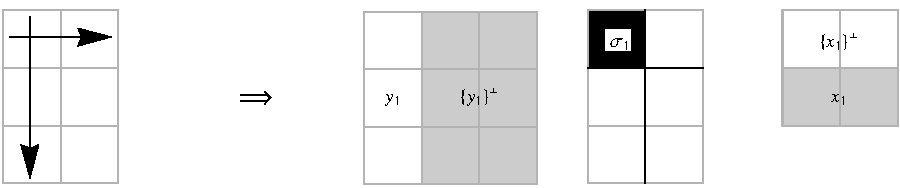
\includegraphics[ width = 5in ]{pdf/post_mortem/earlydecomp.pdf} 
   \caption{A schematic look at the \svdl. In the previous chapter we took a matrix with one linearly independent column vector (down arrow) and one linearly independent row vector (right arrow) and resolved the domain and codomain into four fundamental subspaces shown here.}
   \label{fig:pm:decomp}
\end{figure}

\textbf{Quo vadis?}\\
This chapter will look at the result in a bit more detail. In particular focus will be drawn to which of this spaces are the physical space of measurements and which are the abstract aphysical spaces of the fit parameters.

The last chapter presented a least squares solution using \textit{orthogonal projection}\index{orthogonal projection} to minimize the distance between the measurement vector and the range of the target matrix. Here we connect this result with solution to the normal equations.

%%
\section{Interpretation of the system}
We saw that the linear system in equation \eqref{eq:2:problem} has no solution. There is no possible vector $\xi$ such that
\begin{equation}
  \A{}\xi=\phi.
\end{equation}
Yet we have answer, we found a value for the vector $\xi$. What is the significance of this $2-$vector? Under the mapping action $\A{}$, the $2-$vector in the domain corresponds to the $3-$vector $p=\A{}\xi$ in the codomain. The solution we have constructed minimizes the distance between the data $\phi$ and the image of $\A{}$. 

Put another way, the vector $\xi$ which minimizes the error norm
\begin{equation}
  \normt{\epsilon}^{2} = \normt{\A{}\xi-\phi}^{2}.
\end{equation}
is the orthogonal projection of the data onto the range of $\A{}$. Notice that the minimization occurred in the codomain. The next part of the problem involves the inverse problem: connecting this closest point in the codomain to a point in the domain.

%%
\subsection{The special solution}
We see that the special solution provided by the pseudoinverse,
\begin{equation}
  \A{+}\phi = \xi_{p}
\end{equation}
is the particular solution. The \vvv 
\begin{equation*}
  \A{}\xi_{p} = p
\end{equation*}
is the orthogonal projection of the data onto the range or $\A{}$ and as such is the solution with the minimum $2-$norm.

In some sense, all roads lead to Rome and we could have obtained this same solution using the normal equations, calculus or numerical iteration. The advantage of using the SVD is that we see a clear decomposition of the ranges and null spaces which we can use to visualize the geometry and quality of the solutions. Let's explore these other solution methods.

%%
\subsection{The merit function in parameter space}
In a classic least squares fit, one minimizes a merit function to find the solution. This merit function quantifies the difference between each measurement and the prediction. These differences are called the residual errors. The method of least squares minimizes the sums of the squares of these residual errors. A candidate merit function is
\begin{equation}
  M(\xi) = \normt{\A{}\xi-\phi}^{2} = \paren{\A{}\xi-\phi}^{\mathrm{T}}\paren{\A{}\xi-\phi}.
  \label{eq:merit}
\end{equation}

The plots below show what this merit function looks like. Observe that the merit function takes a $2-$vector as the argument and returns a scalar, a real number. These figures show the solution and how the merit function changes under perturbations of the input variables. The problem with plotting the merit function is seen in the figure. All solutions along the dashed line have the same value for the merit function. Without knowledge of the range of the target matrix we are unable to select any one answer.

\begin{figure}[t] %  figure placement: here, top, bottom, or page
   \centering
   \includegraphics[ width = 3.25in ]{pdf/post_mortem/threed} \\[10pt]
   \includegraphics[ width = 3.25in ]{pdf/post_mortem/contour}
   \caption[Equivalent views of the merit function in parameter space]{Equivalent views of the merit function in parameter space: the domain. The figure on the top is a 3D rendering which reveals the basic shape of the error hypersurface. The contour plot on the bottom is more useful for qualitative analysis. This plot shows the solution $\A{+}\phi$ (white point) and the space resolved into orthogonal coordinates, the image space  $\X{}_{:,1}$ (dashed line) and the null space $\X{}_{:,2}$ (faint dotted line). The merit function does not have a minimum point; the locus of minima is line which defines the null space. space, the dashed line. The intersection of the range space and the minima is the particular solution.}
   \label{fig:2:merit}
\end{figure}
\clearpage


The SVD warned us that we could only minimize the merit function along a line: there was a solitary singular value. The zero eigenvalues signal that the system is inconsistent or underdetermined.

%%s
\section{Solution using the calculus}
The particular solution also comes from a basic calculus problem: minimize the distance between a point and a line. The point is the measurement and the line is the span of the image vector. Of course a concern is that we are not solving the problem with these machinations. We are finding a \vvv \ in the image; we need the \vv \ in domain that maps to this \vvv.

The line represents the fundamental column in $\A{}$ and is parameterized as
\begin{equation}
  \begin{split}
    f(\alpha)=\alpha\mat{r}{1\\-1\\1}.
    \label{eq:range}
  \end{split}
\end{equation}
The square of the $L_{2}$ distance $d_{2}$ between the data and the image is given by
\begin{equation}
  d_{2}^{2}\paren{\phi,f(\alpha)} = \normt{\phivector-\mat{r}{\alpha\\-\alpha\\ \alpha}}^{2} = 3\alpha^{2}-2\alpha+5.
\end{equation}
Minimize this distance in the canonical fashion: set the first derivative equal to zero and solve for $\alpha$. The result is this
\begin{equation}
  \alpha = \frac{1}{3}.
\end{equation}
This implies that the point $p$ on the line $f(\alpha)$ closest to the data point is this
\begin{equation}
  p=\frac{1}{3}\mat{r}{1\\-1\\1}.
  \label{eq:p}
\end{equation}
\begin{figure}[h]
   \centering
   \includegraphics[ ]{pdf/simple/image03.pdf} 
   \caption[The picture in the space of measurements]{The picture in the space of measurements: the image. The thick black line is the range $\rng{\A{}}$ or image of the matrix $\A{}$ given by equation \eqref{eq:range}. The blue arrow represents the measurement vector $\phi$ in equation \eqref{eq:phi}. The least squares solution is the orthogonal projection (red arrow) from the data vector onto the image of the row space. The solution point on the image is also in red and is given in equation \eqref{eq:p}. All of these constructs are shadowed on the floor to help with the perspective. The \vvv \ $p$ is not the solution. The final answer is the \vv \ $\xi_{p}$ which maps to $p$ via $\A{}\xi_{p}=p$. }
   \label{fig:image}
\end{figure}

Notice that the point $p$ is a \vvv \ and therefore a resident of the codomain. The solution must be a \vv \ from the domain. The question now arises: which \vv \ $\xi_{p}$ in the domain connects to the \vvv \ $p$? Mathematically we are solving this equation for $\xi_{p}$:
\begin{equation}
  \A{}\xi_{p}=p.
\end{equation}

Before you lament that we have gone back to the beginning and are solving the same linear system observe that this time there is an exact solution. The data vector $p$ is in the image of  the system matrix $\A{}$. 

Because the system is basic we guess the solution to the equation
\begin{equation}
 \Aexample \mat{c}{\xi\\\eta} = \frac{1}{3}\mat{r}{1\\-1\\1}
\end{equation}
is given by
\begin{equation}
  \mat{c}{\xi\\\eta}=\frac{1}{6}\mat{r}{1\\-1}.
\end{equation}

What if the problem is more complicated? In the case of the normal equations we can depend upon an elimination scheme to provide the solution.

\endinput
\section[The bounty from the SVD]{The bounty from \svdl}
The elegance of the SVD blossoms when we examine the domain and the codomain in terms of contributions from the target matrix to the $\X{}$ and $\Y{}$ matrices shown in table \eqref{tab:vecs}.

\subsection{The row space: home of the solution}
The domain is $\real{2}$ and is resolved into two orthonormal vectors. The first vector comes from the first row vector (the first column in the matrix transpose) and becomes  $\X{}_{*,1}$. The orthogonal complement is \textit{constructed} based upon the first vector. The result becomes $\X{}_{*,2}$.

\subsection{The column space: home of the measurements}
The codomain is $\real{3}$ and requires three orthonormal vectors. The first vector comes from the first column vector in the target matrix and becomes  $\Y{}_{*,1}$. The orthogonal complement is \textit{constructed} based upon the first vector. The result becomes $\Y{}_{*,2}$ and $\Y{}_{*,3}$.

These relationships are shown in table \eqref{tab:vecs}.

\begin{table}[h]
\begin{center}
\boxed{
\begin{tabular}{ccc}
Domain & source & host \\ vector & vector & space \\\hline
$\X{}_{*,1}$ & $\A{T}_{*,1}$ & $\rng{\A{T}}$ \\[3pt]
$\X{}_{*,2}$ & $\paren{\A{T}_{*,1}}^{\perp}$ & $\nll{\A{}}$\\
&\\
$\Y{}_{*,1}$ & $\A{}_{*,1}$ & $\rng{\A{}}$ \\[3pt]
$\Y{}_{*,2}$ & $\paren{\A{}_{*,1}}^{\perp}_{1}$ & $\nll{\A{T}}$ \\[3pt]
$\Y{}_{*,3}$ & $\paren{\A{}_{*,1}}^{\perp}_{2}$ & $\nll{\A{T}}$ \\[5pt]
\end{tabular}
}
\end{center}
\caption{Resolving the domain and codomain into complete orthonormal systems. In this pedagogical example we can see connections between the domain matrices $\X{}$ and $\Y{}$ and the inputs $\A{}$ and $\A{T}$. The \svdl \ has resolved the row and column spaces into complete domains $\real{2}$ and $\real{3}$ by resolving the orthogonal complements.}
\label{tab:vecs}
\end{table}

%%
\section{Before and after}
Consider the issue of the vector spaces before and after the SVD. The row and column spaces are the spans of the linearly independent row and column vectors. When we plot all of the row and column vectors it is clear that each vector space has one linearly independent vector.

Perhaps the shortest summary is in{tab:munificence} which shows the vector spaces for the target matrix before and after the \svdl. We were able to use the first row and column vector for the range vectors. Then the complementary null space vectors were constructed.
\begin{table}[htdp]
\begin{center}
\begin{tabular}{lll}
 & DOMAIN & CODOMAIN \\
 & (Induced by row space) & (Induced by column space) \\\hline\hline
 pre SVD: & $\spn \lst{\mat{r}{1\\-1}}$ & $\spn \lst{\mat{r}{1\\-1\\1}}$ \phantom{$\mat{c}{1\\1\\1\\1}$}\\[5pt]\hline
 post SVD:  & $\underbrace{\spn \lst{\mat{r}{1\\-1}}}_{\rng{\A{T}}} \oplus \underbrace{\spn \lst{\mat{r}{1\\1}}}_{\nll{\A{}}^{\phantom{T}}}$ & $\underbrace{\spn \lst{\mat{r}{1\\-1\\1}}}_{\rng{\A{}}^{\phantom{T}}} \oplus \underbrace{\spn \lst{\veca,\vecb}}_{\nll{\A{T}}}$ \\[35pt]\hline
\end{tabular}
\end{center}
\label{tab:munificence}
\caption{The munificence of the SVD. The target matrix has row and column spaces that are incomplete. The SVD resolves these spaces into complete, orthonormal spaces for the domain and codomain.}
\end{table}

``The completeness of a space'' may seem like an abstract term. It has a concrete meaning. For example, if the host space is $\real{2}$, then a complete space is a vector space which allows access to every point in the plane. If the vector space $\mathcal{V}$ is given as
\begin{equation}
\mathcal{V} = \spn \lst{\mat{r}{1\\-1}}
\end{equation}
then only points along the line including the origin and the point 
\begin{equation}
p=\mat{r}{1\\-1}
\end{equation}
can be accessed. For example, the points 
$$
\mat{r}{2\\-2},\ \mat{r}{3\\-3},\ \mat{r}{\pi\\-\pi},\ \sqrt{2}\mat{r}{-1\\1}
$$
are on this line. The point 
\begin{equation*}
  \mat{r}{1\\0}
\end{equation*}
is not on the line.

A problem with the target matrix is that both the row space and the column space are incomplete. Figures \eqref{fig:2d} and \eqref{fig:3d} show the incomplete row and column spaces represented by the row and column vectors of the target matrix.
\begin{figure}[htbp] %  figure placement: here, top, bottom, or page
   \centering
   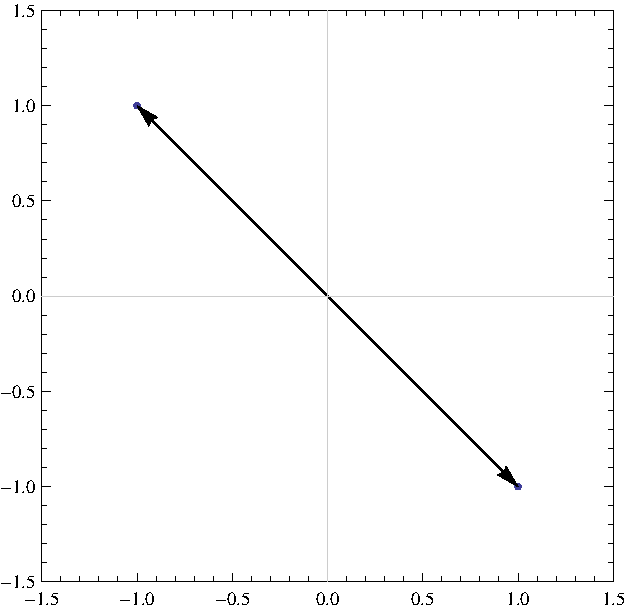
\includegraphics[ width = 2in ]{pdf/post_mortem/2d_before} \qquad
   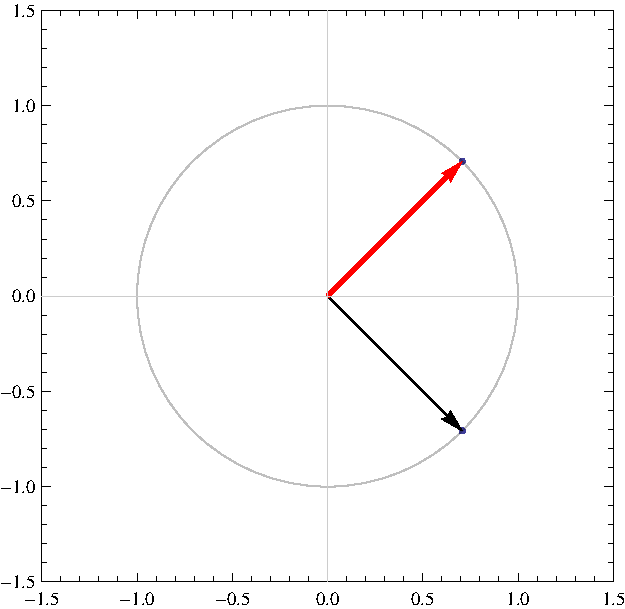
\includegraphics[ width = 2in ]{pdf/post_mortem/2d_after} 
   \caption{The row space before and after the SVD. The row vectors of the target matrix are on the left and the orthonormal resolution of the domain on the right. The null vector which completes the space is shown in red.}
   \label{fig:2d}
\end{figure}

\begin{figure}[htbp] %  figure placement: here, top, bottom, or page
   \centering
   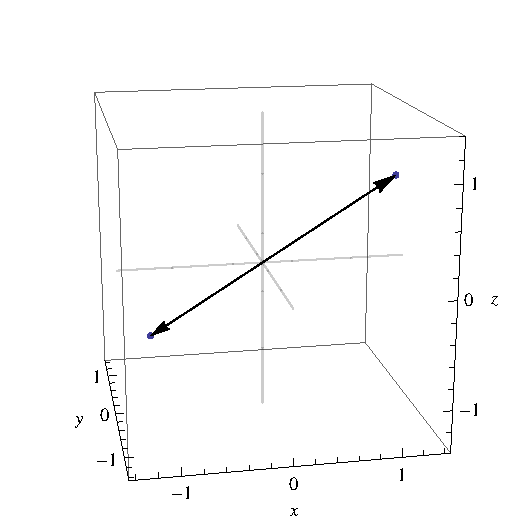
\includegraphics[ width = 2.2in ]{pdf/post_mortem/3d_before} \qquad
   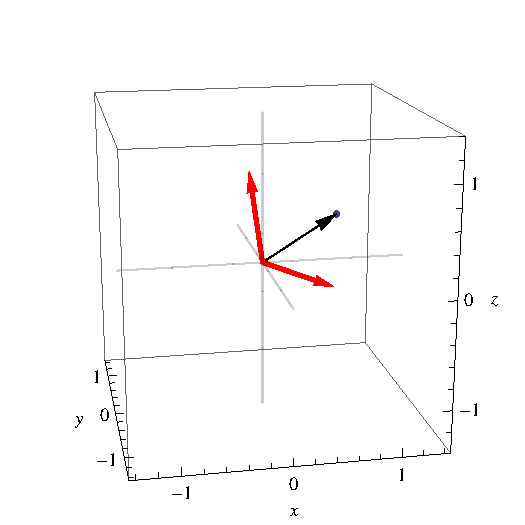
\includegraphics[ width = 2.2in ]{pdf/post_mortem/3d_after} 
   \caption{The column space before and after the SVD. Here too the column space is redundant and incomplete as seen by plotting the column vectors on the left. The orthonormal basis for the complete space is shown on the right.}
   \label{fig:3d}
\end{figure}

%%
\section{The action of the pseudoinverse}
Let's briefly touch on the issue raised in \S\eqref{sec:pi} and look at the product of a matrix and its pseudoinverse. The matrix products are these:

\begin{equation}
  \begin{array}{rcrrcl}
    \leftinv  &=& \Aexample & \Aplus &=& \rthree
    \mat{rrr}
    { 1 & 0 &  1\\
     -1 & \phantom{-}1 & -1\\
      1 & 0 &  1},\\
    \rightinv &=& \Aplus & \Aexample &=& \rtwo
    \mat{rr}
    { 1 & -1\\
     -1 & 1}.\\
  \end{array}
\end{equation}

We will look at another example in \S\eqref{lrfirst} and analyze the situation in the section on chiral inverses \S\eqref{sec:chiral} which will lead to the interpretation in terms of fundamental projectors \S\eqref{sec:orthproj}.

%%
\section{Thin SVD}
Look at the action of the $\sig{}$ matrix holding the singular values. Because of the sabot, the singular values are protected from the null spaces and interact with only the ranges. In effect these paddings prevent the null spaces from contributing the value of the target matrix. It's clear that the null vectors play no role in reconstituting the matrix $\A{}$.

%%
\subsection{An example}
In this context, it makes sense to fashion a \index{thin SVD}\textit{thin SVD} which excludes the null space vectors and the sabot. The thin $\sig{}$ matrix reduces to an $\by{\rho}{\rho}$ diagonal matrix. Using a tilde to denote the thin versions of the product matrices, the thin SVD for the matrix $\A{}$ becomes
\begin{equation}
  \begin{split}
    \A{} &= \svdthin{T},\\
    \Aexample & = \sthree \mat{r}{1\\-1\\1}\mat{c}{\sqrt{6}}\stwo\mat{cc}{1&-1}.
  \end{split}
  \label{eq:thin}
\end{equation}
The dimensions reductions for this problem are these:
$$
\begin{array}{lll}
\text{full SVD} & \svdax{T} & \by{3}{2} = \paren{\by{3}{3}}\paren{\by{3}{2}}\paren{\by{2}{2}} \\
\text{thin SVD} & \A{} = \svdthin{T} & \by{3}{2} = \paren{\by{3}{1}}\paren{\by{1}{1}}\paren{\by{1}{2}} \\
\end{array}
$$

Figure \eqref{fig:thin} displays the SVD before and after losing the null space vectors. Correlate this diagram to equation \eqref{eq:thin}.
\begin{figure}[htbp] %  figure placement: here, top, bottom, or page
   \centering
   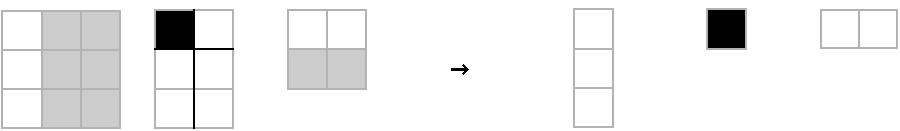
\includegraphics[ width = 5in ]{pdf/post_mortem/thin} 
   \caption{The secret to a thin SVD - lose the null spaces and the sabot. Matrices with incomplete row or column spaces are the only matrices that will shrink under the thin SVD.}
   \label{fig:thin}
\end{figure}

%%
\subsection{The general case}
As you might surmise, the dimensions and rank of the target matrix fully specify the dimensions for both the SVD and the thin SVD. The difference is the null space vectors; the lower the rank the thinner the ``thin SVD''. For a matrix 
\begin{equation}
  \A{}\in \mathbb{C}^{\by{m}{n}}_{\rho}
\end{equation}
the dimensions are given below in table \eqref{tab:bounty:thinsvd}.

\begin{table}[htdp]
\begin{center}
\begin{tabular}{llll}
SVD\quad & formulation & dimensions & size is rank\dots \\\hline
full & $\svd{*}$ & $\by{m}{n} = \paren{\by{m}{m}}\,\paren{\by{m}{n}}\,\paren{\by{n}{n}}$ & independent \\
thin & $\svdthin{*}$ & $\by{m}{n} = \paren{\by{m}{\rho}}\,\paren{\by{\rho}{\rho}}\,\paren{\by{\rho}{n}}$ & dependent \\[10pt]
\end{tabular}
\end{center}
\label{tab:bounty:thinsvd}
\caption{A comparison between the sizes of the component matrices for a full and thin SVD. Essentially, the thin SVD omits the null space vectors.}
\end{table}%

\endinput
\section{Exercises}
\begin{enumerate}
\item Consider the SVD given for $\Arrr{2}{2}{2}$:
\begin{equation*}
  \svdax{T} = 
  \mat{c|c}{y_{11} & y_{12} \\ y_{21} & y_{22}}
  \mat{cc}{\sigma_{1} & 0 \\ 0 & \sigma_{1}}
  \mat{cc}{x_{11} & x_{12} \\\hline x_{21} & x_{22}}.
\end{equation*}
Show by direct computation of the product that
\begin{equation*}
\begin{split}
  \A{} 
  &= \mat{cc}{
  \sigma_{1} x_{11} y_{11} + \sigma_{2} x_{12} y_{12} & \sigma_{1} x_{21} y_{11} + \sigma_{2} x_{22} y_{12} \\
  \sigma_{1} x_{11} y_{12} + \sigma_{2} x_{12} y_{22} & \sigma_{1} x_{21} y_{12} + \sigma_{2} x_{22} y_{22} } \\
  &= \sigma_{1} \mat{cc}{
  y_{11} \mat{cc}{x_{11} & x_{21}} \\
  y_{12} \mat{cc}{x_{11} & x_{21}}}
  + \sigma_{2} \mat{cc}{
  y_{21} \mat{cc}{x_{12} & x_{22}} \\
  y_{22} \mat{cc}{x_{12} & x_{22}}} \\
  &= \sigma_{1} y_{1}x_{1}^{T} + \sigma_{2} y_{2}x_{2}^{T}.
\end{split}
\end{equation*}
\item
\item
\end{enumerate}


\endinput

\endinput
\chapter[SVD with eigenvalues]{General case: SVD with eigenvalues}
\label{chap:general}
The general method for finding the \svdp \ demands finding the eigenvalues of either product matrix, $\W{x}$ or $\W{y}$. As we will see later, every matrix has a \svdl, and so having a robust general method guarantees that we can resolve every matrix into the component matrices.

%%
\section{Comparing two SVD strategies}
In the previous chapter we saw a quick and pedagogical method for composing an SVD. It clearly demonstrated the resolution of the domain and codomain and emphasized the elementary nature of the decomposition.

However, there are some shortcomings to the method: 
\begin{enumerate}
\item the essence of the singular values is obscured;
\item the method is not universal.
\end{enumerate}

While both methods rely upon augmented reduction, the general method also requires solving an eigensystem.

Table \eqref{tab:3:comparex} compares the simple method of the first chapter with the general method that we are about to explore. In this form the differences in strategy seem innocuous. In fact, the conception of the general method is comparable to the conception of the simple method. However, the general method requires solving an eigensystem. It is the resolution of the eigenvalues and eigenvectors for the product matrix that can make practical decompositions so daunting. 

\begin{table}[h]
\begin{center}
\begin{tabular}{l|cclll }
 & {\it construct} & {\it solve for} & {\it method} & {\it pros} & {\it cons} \\ \hline
 1 & $\X{}$, $\Y{}$ & $\Sigma$ & augmented reduction & easy & special cases \\[3pt]
 2 & $\X{}$, $\Sigma$ & $\Y{}$  & eigenvalue problem  & difficult & universal \\[3pt]\hline
\end{tabular}
\end{center}
\label{tab:3:comparex}
\caption{Comparing two strategies for the SVD. The easy method of chapter 1 is on top; the general method on the bottom.}
\end{table}%

%%
\section[The general method for SVD]{The general method for \svdl}

This chapter focuses on the most general method for computing an SVD. The requisite steps are elementary, but the combination of tasks can obscure the process. To minimize this \index{fog of computation}fog of computation the process is dissected and mounted in equation \eqref{eq:gen:flow} and tables \eqref{tab:3:} and \eqref{tab:3:input}. The tables are for reference.

%%
\begin{landscape}
\thispagestyle{empty}

\begin{equation}
  \begin{array}{ccccccccccccc}
  \A{}&\longrightarrow&\A{*}&\longrightarrow&\W{x}&\longrightarrow&\lambda\paren{\W{x}}&\longrightarrow&\lst{\sigma_{k}}&\longrightarrow&\sig{}\\
  &&&&\downarrow\\
  &&&&\lst{x_{k}}&\longrightarrow&\lst{x_{k}}^{\perp}&\longrightarrow&\X{}\\
  &&&&&&&&\downarrow\\
  &&&&&&&&\lst{y_{k}}&\longrightarrow&\lst{y_{k}}^{\perp}&\longrightarrow&\Y{}\\
  \end{array}
  \label{eq:gen:flow}
\end{equation}
Flow chart for a typical \svdl. This layout shows the simplicity of the underlying decomposition process. In general, it is the eigenvalue problem thats gives the SVD a reputation as being difficult.

To compute:
\begin{enumerate}
\item $\A{*}$, the Hermitian conjugate: compute $\overline{\A{}}^{\mathrm{T}}$;
\item $\W{x}$, the product matrix: compute $\prdm{*}$;
\item $\lambda(\W{x})$, the eigenvalue spectrum: solve $p(\lambda)=0$; i.e. find the $\rho$ nonzero roots of the characteristic polynomial;
\item $\lst{\sigma_{k}}, \  k=1,\rho$, the singular values of $\A{}$: arrange the nonzero products $\sqrt{\lambda}$ in descending order;
\item $\sig{}$, the matrix of singular values: embed the singular values along the diagonal of the sabot matrix of zeros;
\item $\lst{x_{k}},\  k=1,\rho$, the eigenvectors of $\W{x}$: find the null space vectors of $\W{x}-\lambda_{k}\I{n},\  k=1,\rho$;
\item $\lst{x_{k}}^{\perp},\  k=\rho+1,n$, the orthonormal perpendicular complement to $\lst{x_{k}}$: use the Gram-Schmidt process;
\item $\X{}$, the orthonormal basis matrix for the domain: arrange the vectors as $\X{}=\mat{c|c}{x_{k} & x^{\perp}_{j}}, \  k=1,\rho, \ j = \rho+1,n$;
\item $\lst{y_{k}},\  k=1,\rho$, the eigenvectors of $\W{y}$: compute $y_{k} = \sigma_{k}^{-1}\A{}x_{k},\  k=1,\rho;$
\item $\lst{y_{k}}^{\perp},\  k=\rho+1,m$, the orthonormal perpendicular complement to $\lst{y_{k}}$: use the Gram-Schmidt process;
\item $\Y{}$, the orthonormal basis matrix for the codomain: arrange the vectors as $\Y{}=\mat{c|c}{y_{k} & y^{\perp}_{j}}, \  k=1,\rho, \ j = \rho+1,m$.
\end{enumerate}

\clearpage
\thispagestyle{empty}

%%
\begin{table}[p]
\begin{center}
\begin{tabular}{lllcll}
 symbol & type & size & census & description & use \\\hline
 $\A{}$ & matrix & $\cmplx{\by{m}{n}}_{\rho}$ & 1 & target matrix  & input matrix \\
 $\A{*}$ & matrix & $\cmplx{\by{n}{m}}_{\rho}$ & 1 & Hermitian conjugate & intermediate matrix\\ 
 $\W{x}$ & matrix & $\cmplx{\by{n}{n}}_{\rho}$ & 1 & product matrix $\A{*}\A{}$ & intermediate matrix\\
 $\W{y}$ & matrix & $\cmplx{\by{m}{m}}_{\rho}$ & 1 & product matrix $\A{}\A{*}$ & intermediate matrix \\
 \ &&& \\
 $x_{k}$ & $n-$vectors & $\cmplx{\by{n}{1}}$ & $\rho$ & eigenvectors of $\W{x}$ & first $\rho$ columns of $\X{}$ \\
 $y_{k}$ & $m-$vectors & $\cmplx{\by{m}{1}}$ & $\rho$ & eigenvectors of $\W{y}$, $\paren{\sigma_{k}}^{-1}\A{}\X{}_{:,k}$ & first $\rho$ columns of $\Y{}$ \\
 $\paren{x_{k}}^{\perp}$ & $n-$vectors & $\cmplx{\by{n}{1}}$ & $n-\rho$ & orthogonal null space vector, domain & remaining $n-\rho$ columns of $\X{}$ \\
 $\paren{y_{k}}^{\perp}$ & $m-$vectors & $\cmplx{\by{m}{1}}$ & $m-\rho$ & orthogonal null space vector, codomain & remaining $m-\rho$ columns of $\Y{}$ \\
 \ &&& \\
 $\lambda_{k}$ & reals && $\rho$ & eigenvalues of the smaller of $\W{x}$, $\W{y}$ &intermediate product \\
 $\sigma_{k}$ & reals && $\rho$ & singular values $\sqrt{\lambda_{k}}$ & diagonal elements of $\sig{}$\\
 \ &&& \\
  $\ess{}$ & matrix & $\real{\by{\rho}{\rho}}_{\rho}$ & 1 & singular values matrix & intermediate matrix \\
  $\sig{}$ & matrix & $\real{\by{m}{n}}_{\rho}$ & 1 & $\sig{}$ matrix & output matrix \\
  $\X{}$ & matrix & $\cmplx{\by{n}{n}}_{n}$ & 1 & unitary domain matrix & output matrix \\
  $\Y{}$ & matrix & $\cmplx{\by{m}{m}}_{m}$ & 1 & unitary codomain & output matrix \\
[10pt]
\end{tabular}
\end{center}
\label{tab:3:personaedramatis}
\caption{Personae dramatis. This is a directory detailing the inputs, outputs and intermediary quantities used to find an SVD. The column vectors of the domain matrices $\X{}$ and $\Y{}$ are orthonormal.}
\end{table}

\end{landscape}
\clearpage
\break
%%
\begin{table}[h]
Given $\A{}\in\cmplx{\by{m}{n}}_{\rho}$, a matrix of rank $\rho$ with $m$ columns and $n$ rows, compute the \svdl \ $\A{}=\Y{}\,\Sigma\,\X{*}$ using these steps:\\[4pt]
\begin{enumerate}
\item Compute $\A{*}$, the conjugate of the transpose.\\[4pt]
\item Compute $\W{x}=\prdm{*}$.\\[4pt]
\item Solve for the $\rho$ ordered, nonzero eigenvalues $\lambda_{k}$ of $\W{x}$.\\[4pt]
\item Compute the $\rho$ singular values $\sigma_{k}=\sqrt{\lambda_{k}}, \ k=1,\rho$.\\[4pt]
\item Assemble $\sig{}$ the matrix of singular values. It is a sabot matrix of zeros with the $\rho$ singular values $\sigma_{k}$ on the diagonal in descending order.
\begin{equation}
  \Sigma = \underbrace{\mat{cccccccc}
  {
  \sigma_{1} & 0 & 0 & \cdots &&&& 0\\
  0 & \sigma_{2} & 0 & \dotsm &&&& 0\\
  0 & 0 & \ddots &&&&& \vdots \\
  \vdots & \vdots & & \sigma_{\rho} \\
   &  & & & 0  \\
   &  & & & & \ddots  \\
  0 & 0 &  & \cdots &&&& 0
  }}_{n \text{ columns}}
  \left. \phantom{\begin{array}{l}
  1\\
  1\\
  1\\
  1\\
  1\\
  1\\
  1\\
  1\\
  1
  \end{array}}\right\}
  m\text{ rows}.
\end{equation}
\item Solve for the $\rho$ eigenvectors $x_{k}$ of $\W{x}$.\\[4pt]
\item Compute $\tau_{x}=n-\rho$ orthonormal null space vectors for the perpendicular complement of the space spanned by these eigenvectors, $\lst{x}^{\perp}=\spn\lst{u_{1},\dots,u_{\tau_{x}}}$.\\[4pt]
\item Assemble the $\by{n}{n}$ matrix 
$\X{}=\mat{c|c|c|c|c|c}
{\hat{x}_{1} & \cdots & \hat{x}_{\rho} & \hat{u}_{1} & \dots & \hat{u}_{\tau_{x}}
}
$
for the domain.\\[4pt]
\item Solve for the $\rho$ vectors $y_{k}$, the orthonormal decomposition of $\rng{\A{}}$, using
\begin{equation}
  y_{k} = \paren{\sigma_{k}}^{-1}\A{} x_{k}.
\end{equation}
\item Compute $\tau_{y}=m-\rho$ null space vectors which are the  orthonormal perpendicular to the image space $\lst{y}^{\perp}=\spn\lst{v_{1},\dots,v_{\tau_{x}}}$ for the codomain.\\[4pt]
\item Assemble the $\by{m}{m}$ matrix 
$\Y{}=\mat{c|c|c|c|c|c}
{\hat{y}_{1} & \cdots & \hat{y}_{\rho} & \hat{v}_{1} & \dots & \hat{v}_{\tau_{y}}
}
$ for the codomain.\\[4pt]
\item Verify $\svd{*} = \A{}.$\\[6pt]
\end{enumerate}
\caption{Recipe for a \svdl. These are the basic tasks for the general purpose method to complete the full SVD. As with any recipe, there are variants. The simple method in the last chapter is one such variant. Consider these steps to be the most robust and general method. A hat over a vector implies normalization.}
\label{tab:3:input}
\end{table}

\clearpage
\break

\endinput
\section{The matrix of singular values}

In this volume we have, by fiat, restricted the singular values to being nonzero. This is a convention, by no means a theoretical necessity.


\begin{table}[htdp]
\begin{center}
\begin{tabular}{lccc|cc}
  $\A{}$ & $\sig{}$ & $\sig{T}$ & $\sig{(+)}$ & $\sig{}\sig{(+)}$ & $\sig{(+)}\sig{(+)}$\\
  $\cmplx{\bys{2}}_{2}$ &
  $\mat{cc}{\sigma_{1}&0\\0&\sigma_{2}}$ & 
  $\mat{cc}{\sigma_{1}&0\\0&\sigma_{2}}$ & 
  $\mat{cc}{\frac{1}{\sigma_{1}}&0\\0&\frac{1}{\sigma_{2}}}$ & $\itwo$ & 
  $\itwo$\\ 
  %%
  $\cmplx{\by{3}{2}}_{2}$ &
  $\mat{cc|c}{\sigma_{1}&0&0\\0&\sigma_{2}&0}$ & 
  $\mat{cc}{\sigma_{1}&0\\0&\sigma_{2}\\\hline 0&0}$ & 
  $\mat{cc}{\frac{1}{\sigma_{1}}&0\\0&\frac{1}{\sigma_{2}}\\[3pt]\hline 0&0}$ &
  $\itwo$ & 
  $\mat{cc|c}{1&0&0\\0&1&0}$\\
  %%
  $\cmplx{\by{2}{3}}_{1}$ &
  $\mat{c|c}{\sigma_{1}&0\\\hline0&0\\0&0}$ & 
  $\mat{c|cc}{\sigma_{1}&0&0\\\hline0&0&0}$ & 
  $\mat{c|cc}{\frac{1}{\sigma_{1}}&0&0\\[3pt]\hline0&0&0}$ &
  $\mat{c|cc}{1&0&0\\\hline0&0&0\\0&0&0}$ & 
  $\mat{c|c}{1&0\\\hline0&0}$ \\
  \ \\
\end{tabular}
\end{center}
\caption{Different forms for the $\sig{}$ matrix for three types of matrices. The matrices $\sig{}$ and $\sig{T}$ share the same diagonal; $\sig{T}$ and $\sig{(+)}$ share the same shape.}
\label{tab:sing}
\end{table}%

Stencils
truncated identity
\begin{equation}
  \begin{split}
    \sig{}\sig{(+)} &= \mat{c|c}{\I{m}&\zero\\\hline\zero&\zero} = \J{m}{\rho}, \\
    \sig{(+)}\sig{} &= \mat{c|c}{\I{n}&\zero\\\hline\zero&\zero} = \J{n}{\rho}.
  \end{split}
\end{equation}


\endinput
\section{The problem}
Apply the general method to the new target matrix
\begin{equation}
  \A{} = \mat{ccc}
  {
  0 & 3 & 0 \\
  1 & 2 & 2
  }
\end{equation}
and follow the steps in table \eqref{tab:3:input} to produce an SVD.\\

Diagnosis: the target matrix has rank 2 due to two independent rows. Therefore we can define the shapes of the component matrices as show in figure \eqref{fig:232}.
\begin{equation}
  \A{}\in\real{\by{2}{3}}_{2}.
\end{equation}
\begin{figure}[htbp] %  figure placement: here, top, bottom, or page
   \centering
%   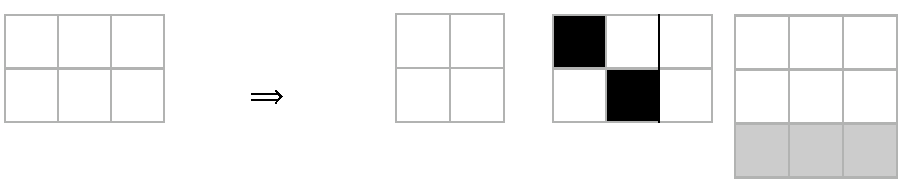
\includegraphics[ ]{pdf/general/svd_02_03_02} 
   \includegraphics[ ]{pdf/general/C232} 
   \caption[Shapes and dimensions]{The shapes and dimensions for the pending decomposition are determined by the shape of the target matrix. The rank tells us how many singular values we will find.}
   \label{fig:232}
\end{figure}
%%%

%%
\subsection{Compute the adjoint matrix $\A{T}$}
\begin{equation}
  \A{} = \mat{cc}
  {
  0 & 1 \\
  3 & 2 \\
  0 & 2
  }.
\end{equation}

%%
\subsection{Compute the product matrix $\W{x}$}
\begin{equation}
  \W{x}=\A{T}\A{}= \mat{ccc}{
 1 &  2 & 2 \\
 2 & 13 & 4 \\
 2 &  4 & 4}
\label{eq:problemgen:Wx}
\end{equation}

%%
\subsection{Find the eigenvalues of $\W{x}$}
We could solve this system for eigenvectors and eigenvalues. But the product matrix $\W{y}$ is a smaller and simpler system to resolve. So to reduce the amount of labor we will work with the other product matrix
\begin{equation}
  \W{y}=\A{}\,\A{T} =
\left[
\begin{array}{cc}
 9 & 6 \\
 6 & 9
\end{array}
\right].
\label{eq:problemgen:Wy}
\end{equation}
Details are in the appendix allowing a freedom to touch upon just the high notes. 

Start with a some simplification: remove common factors from the product matrix. To wit
\begin{equation}
  \W{y}=3\W{y}'.
  \label{eq:scale}
\end{equation}

To find the eigenvalues, find the the roots of the \index{characteristic polynomial} characteristic polynomial defined by
\begin{equation}
  p(\lambda) = \det \paren{\W{y}'-\lambda \I{2}} =
  \det \mat{cc}
  {
  3-\lambda & 2 \\
  2 & 3-\lambda
  }.
\end{equation}

In this instance we find
\begin{equation}
  p(\lambda) = \lambda^{2} - 6\lambda + 5
\end{equation}
which is easily factored. Extracting the roots to $p(\lambda) = 0$ yields $\lambda = \lst{5,1}$. Accounting for the scale factor in \eqref{eq:scale} we say the eigenvalue spectrum for the product matrix $\W{y}$ is given by
\begin{equation}
  \lambda = \lst{15, 3}
\end{equation}

\textbf{Caution:} Always arrange the eigenvalues in \textit{decreasing} magnitude.

%%
\subsection{Compute the singular values $\sigma_{k}$}
The singular values are the square root of the non-zero eigenvalues of the product matrices:
\begin{equation}
  \sigma = \sqrt{\lambda} = \lst{\sqrt{15},\sqrt{3}}.
\end{equation}

%%
\subsection{Build the $\sig{}$ matrix}
The $\sig{}$ matrix of singular values has the same dimensions are the target matrix. Populate the upper diagonal with singular values:
\begin{equation}
  \A{} = \mat{cc|c}
  {
  \sqrt{15} & 0 & 0 \\
  0 & \sqrt{3}  & 0
  }
\end{equation}

%%
\subsection{Find the eigenvectors of the product matrix $\W{x}$}
The eigenvalue problem for this example is this
\begin{equation}
  \W{x}\lambda_{k} = \lambda_{k} x_{k}, \quad k=\lst{1,\rho}.
  \label{eq:raw:ev}
\end{equation}
Here $x_{k}$ is the eigenvector of interest. Notice that we skip any cases where $\lambda=0$. Yes, this would provide null vectors, but they would not be an orthogonal set.

The canonical method for solving equation \eqref{eq:raw:ev} is to express it as a null space problem as they are easier to solve:
\begin{equation}
  \paren{\W{x} - \lambda_{k}\I{3}} = \zero, \quad k=\lst{1,\rho}.
\end{equation}
The two cases follow. Both will be solved by augmented reduction or EAR.
\begin{enumerate}
\item For $k=1$. The source matrix is given by
\begin{equation}
\W{x}-15\I{3} =
\left[
\begin{array}{rrr}
 -14 & 2 & 2 \\
 2 & -2 & 4 \\
 2 & 4 & -11
\end{array}
\right]. 
\end{equation}
The augmented system has this final form
\begin{multline}
\frac{1}{12}
\left[
\begin{array}{rrr}
 5  & 29 & 12 \\
 -1 & -7 & 0 \\
 6  & 30 & 12
\end{array}
\right]
\mat{rrr|ccc}
{
-14 & 2 & 2 & 1 & 0 & 0 \\
 2 & -2 & 4 & 0 & 1 & 0 \\
 2 & 4 &-11 & 0 & 0 & 1
}\\
=
\mat{crr|rrc}
{
1 & 0 & -\frac{1}{2}  &  \frac{5}{12} & \frac{29}{12} & 1 \\
0 & 1 & -\frac{5}{2}  & -\frac{1}{12} & -\frac{7}{12} & 0 \\[4pt]\hline\hline
0 & 0 & 0             &  \frac{1}{2}  & \frac{5}{2}   & 1
}.
\end{multline}
The double horizontal lines are drawn to accentuate the boundary of the null vectors. The row vectors of interest accompany the zero vectors on the bottom of the matrix on the right. In this case there is just one vector:
\begin{equation}
  x_{1}^{\mathrm{T}} = \mat{ccc}{1&5&2}
\end{equation}
After normalization, we have the first column in the domain matrix:
\begin{equation}
  \X{}_{*,1} = \hat{x}_{1} = \frac{1}{\sqrt{30}}\mat{c}{1\\5\\2}.
\end{equation}
\item For $k=2$
\begin{equation}
\W{x}-3\I{3} =
\left[
\begin{array}{rrr}
 -2 & 2 & 2 \\
 2 & 10 & 4 \\
 2 & 4 & 1
\end{array}
\right].
\end{equation}
The augmented system has this final form
\begin{multline}
\frac{1}{12}
\left[
\begin{array}{crc}
 1 & -5 & 12 \\
 1 &  1 & 0 \\
 6 & -6 & 12
\end{array}
\right]
\mat{rrr|ccc}
{
-2 & 2  & 2 & 1 & 0 & 0 \\
 2 & 10 & 4 & 0 & 1 & 0 \\
 2 & 4  & 1 & 0 & 0 & 1
}\\
=
\mat{ccr|crc}
{
1 & 0 & -\frac{1}{2}  &  \frac{1}{12} & -\frac{5}{12} & 1 \\
0 & 1 &  \frac{1}{2}  &  \frac{1}{12} &  \frac{1}{12} & 0 \\[4pt]\hline\hline
0 & 0 & 0             &  \frac{1}{2}  & -\frac{1}{2}  & 1
}.
\end{multline}
\end{enumerate}
With normalization, we have the second column in the domain matrix:
\begin{equation}
  \X{}_{*,2} = \hat{x}_{2} = \frac{1}{\sqrt{6}}\mat{r}{1\\-1\\2}.
\end{equation}

%%
\subsection{Construct a null space for the domain}
Part of the confusion about the decomposition comes from the wonderful fact that there are some permutations in the path and multiple ways to approach some steps.

Here there are different ways to construct this third vector and assure that it is perpendicular to the first two vectors. We choose to use the cross-product.

The cross-product between two \vvv s is computed as this
\begin{equation}
\mat{c}{x_{1}\\x_{2}\\x_{3}}
\times
\mat{c}{y_{1}\\y_{2}\\y_{3}}
=
\det
\mat{ccc}
{
\hat{i} & \hat{j} & \hat{k} \\
  x_{1} & x_{2}   & x_{3}   \\
  y_{1} & y_{2}   & y_{3}   \\
}
=
\mat{c}
{
x_{2}y_{3}-x_{3}y_{2} \\
x_{3}y_{1}-x_{1}y_{3} \\
x_{1}y_{2}-x_{2}y_{1} 
}.
\end{equation}
The solitary null space vector is
\begin{equation}
u_{1} = x_{1} \times x_{2} =
\mat{c}{1\\5\\2}
\times
\mat{r}{1\\-1\\2}
=
\mat{r}
{
 2 \\
 0 \\
-1 
}.
\end{equation}
Therefore
\begin{equation}
  \X{}_{*,3} =\hat{u}_{1} = \frac{1}{\sqrt{5}}
\mat{r}
{
 2 \\
 0 \\
-1 
}.
\end{equation}

%%
\subsection{Assemble the domain matrix $\X{}$}
The normalization busies the appearance:
\begin{equation}
  \X{} = 
\left[
\begin{array}{ cr >{\columncolor{ltgray}}r }
  \frac{1}{\sqrt{30}} & \frac{ 1}{\sqrt{6}} & \frac{-2}{\sqrt{5}}\\
  \frac{5}{\sqrt{30}} & \frac{-1}{\sqrt{6}} & 0 \\
  \frac{2}{\sqrt{30}} & \frac{ 2}{\sqrt{6}} & \frac{ 1}{\sqrt{5}}\\
\end{array}
\right].
\end{equation}

A useful alternative presentation of this matrix is to write it as column vectors as shown here:
\begin{equation}
\X{}=
  \mat{c|c|>{\columncolor{ltgray}}c}
  {
  \frac{1}{\sqrt{30}} \mat{r}{1\\5\\2} &
  \frac{1}{\sqrt{6}}  \mat{r}{1\\-1\\2} &
  \frac{1}{\sqrt{5}}  \mat{r}{2\\0\\1}
  }.
\end{equation}
This defeats the camouflage of the normalization constants and reminds us of the significance of the columns. It also simplifies the visual check of orthogonality.

%%
\subsection{Solve for $y_{k}$}
A vital formula needed for \index{jumping between domains}jumping between domain and codomain is this
\begin{equation}
  \A{}\X{}_{*,k} = \sigma_{k} \Y{}_{*,k}, \quad k=\lst{1,\rho}.
  \label{eq:vital}
\end{equation}
\begin{enumerate}
\item For $k=1$
For the first normalized vector in the codomain we need to solve
\begin{equation}
  \begin{split}
    \A{}\X{}_{*,1} &= \sigma_{1} \Y{}_{*,1}, \\
    \mat{ccc}
    {0 & 3 & 0\\
     1 & 2 & 2
    }
    \frac{1}{\sqrt{30}}
    \mat{c}{1\\5\\2}
    & = 
    \sqrt{15} \Y{}_{*,1}.
  \end{split}
\end{equation}
The solution is
\begin{equation}
  \Y{}_{*,1} = \frac{1}{\sqrt{2}}\mat{c}{1\\1}.
\end{equation}
\item For $k=2$
It may be tempting to guess the second and final vector in the codomain matrix; there are only two possible choices. But to do so would entail the risk of placing the minus sign in the wrong place. So much of the decomposition keeps the arbitrary signs in consistent use. After working out the details, the solution to
\begin{equation}
  \A{}\X{}_{*,2} = \sigma_{2} \Y{}_{*,2}
\end{equation}
is the vector
\begin{equation}
  \Y{}_{*,2} = \frac{1}{\sqrt{2}}\mat{r}{-1\\1}
\end{equation}
\end{enumerate}

%%
\subsection{Construct a null space for the codomain}
There is no null space for the codomain; the target matrix has full row rank.

%%
\subsection{Assemble the codomain matrix $\Y{}$}
The codomain matrix is given by
\begin{equation}
  \Y{} = \frac{1}{\sqrt{2}}
  \mat{rr}{1 & -1\\1 & 1}.
\end{equation}

%%
\subsection{Assemble and verify the decomposition}
The formal decomposition is
\begin{equation}
  \boxed{
  \begin{array}{ccccc}
    \A{} &=& \Y{} & \sig{} & \X{T}\\
  \mat{ccc}
  {
  0 & 3 & 0 \\
  1 & 2 & 2
  } 
  &=&
  \frac{1}{\sqrt{2}}
  \mat{rr}{1 & -1\\1 & 1}
  &
  \mat{cc|c}
  {
  \sqrt{15} & 0 & 0 \\
  0 & \sqrt{3}  & 0
  }
  &
  \mat{ crr }
 {\frac{1}{\sqrt{30}} & \frac{5}{\sqrt{30}} & \frac{2}{\sqrt{30}}\\
  \frac{ 1}{\sqrt{6}} & \frac{-1}{\sqrt{6}} & \frac{2}{\sqrt{6}} \\
  \rowcolor{ltgray}
  \frac{-2}{\sqrt{5}} & 0 & \frac{1}{\sqrt{5}}}\\[25pt]
  \end{array}.
  }
  \label{eq:general:ysxt}
\end{equation}

The best way to insure that all the signs on the entries in the domain matrices are correct is to verify the decomposition:
\begin{equation}
  \begin{split}
    \A{} &= \Y{}\paren{\sig{}\,\X{T}},\\
     &=
  \stwo
  \mat{rr}{1 & -1\\1 & 1}
  \paren{
  \stwo
  \mat{crc}
  {
  1 & 5  & 2 \\
  1 & -1 & 2
  }}, \\
  &=
  \mat{ccc}
  {
  0 & 3 & 0 \\
  1 & 2 & 2
  }.
  \end{split}
  \label{eq:gen:soln}
\end{equation}

\endinput
\section{Observations}
We have experienced the full process of \svdl, a series of basic steps. 

The options at many steps which allow easier decomposition confuse some practitioners. These options may be mistakenly juggled with path variations and the SVD process may seem hazy as a result. Keep these things straight in your mind:
\begin{enumerate}
\item Know what you are trying to do;
\subitem resolve the domain and codomain into orthonormal coordinate systems;
\subitem resolve the singular values.
\item Know the foundation issues;
\subitem the row and vector spaces may not fully span the host space;
\subitem the row and column vectors may be far from orthogonal.
\item Remember how to perform each step;
\subitem know how to find eigenvalues and eigenvectors using augmented reduction or other techniques;
\subitem know how to construct perpendicular spaces;
\subitem know how to construct and load the matrix of singular values.
\end{enumerate}

The examples here are pedagogic and illuminate the process and the machinations. Many useful matrices will quickly submit to a \svdl. Hence these theoretical examples are both helpful and useful. However, the decomposition is intractable for many matrices.

Eigenvector problems can be arbitrarily complex. The space may be incomplete and finding mother-daughter eigenvector pairs become a permutation problem which grows factorially. This can be a major impediment.

There are many excellent texts and on-line resources to help with the machinations of finding eigenvalues and constructing orthogonal complements. A survey is listed here:

\begin{table}[htdp]
\begin{center}
\boxed{
\begin{tabular}{lcccc}
  topic & Anton [] & Strang1 [] & Strang2 [] & Meyer [] \\\hline
  augmented reduction & pp. 10-20 & pp. 10-20 & pp. 10-20 & p. 118\\
  eigenvectors & pp. 10-20 & pp. 10-20 & pp. 10-20 & p. 489\\
  null spaces  & pp. 10-20 & pp. 10-20 & pp. 10-20 & p. 173
\end{tabular}
}
\end{center}
\label{default}
\caption{Resources to help with facets of the \svdl.}
\end{table}


\endinput
\section{Exercises}
\begin{enumerate}
\item Consider the SVD given for $\Arrr{2}{2}{2}$:
\begin{equation*}
  \svdax{T} = 
  \mat{c|c}{y_{11} & y_{12} \\ y_{21} & y_{22}}
  \mat{cc}{\sigma_{1} & 0 \\ 0 & \sigma_{1}}
  \mat{cc}{x_{11} & x_{12} \\\hline x_{21} & x_{22}}.
\end{equation*}
Show by direct computation of the product that
\begin{equation*}
\begin{split}
  \A{} 
  &= \mat{cc}{
  \sigma_{1} x_{11} y_{11} + \sigma_{2} x_{12} y_{12} & \sigma_{1} x_{21} y_{11} + \sigma_{2} x_{22} y_{12} \\
  \sigma_{1} x_{11} y_{12} + \sigma_{2} x_{12} y_{22} & \sigma_{1} x_{21} y_{12} + \sigma_{2} x_{22} y_{22} } \\
  &= \sigma_{1} \mat{cc}{
  y_{11} \mat{cc}{x_{11} & x_{21}} \\
  y_{12} \mat{cc}{x_{11} & x_{21}}}
  + \sigma_{2} \mat{cc}{
  y_{21} \mat{cc}{x_{12} & x_{22}} \\
  y_{22} \mat{cc}{x_{12} & x_{22}}} \\
  &= \sigma_{1} y_{1}x_{1}^{T} + \sigma_{2} y_{2}x_{2}^{T}.
\end{split}
\end{equation*}
\item
\item
\end{enumerate}


\endinput

\endinput
\chapter{Post Mortem II}

The previous chapter introduced the general method for resolving a matrix into its \svdl. This method involved finding the singular values by resolving the eigensystem of a product matrix. The next section explores the geometry of the eigenvalues and motivates the perception that the singular values are a set of scale factors.

However, because of the weight of the details in the last chapter, we will exhibit another example. This will provide more insight into the geometry of the singular values.

The trouble with the target matrix in the preceding example is that while it does have enough linearly independent column vectors to span the domain it lacks enough linearly independent row vectors to span the codomain. Therefore there is a left inverse but no right inverse. Therefore the linear system can't be solved using obvious methods again we need the SVD.
 
%%
\section{Solution using the SVD}
Let's return to using an SVD to solve the linear systems like $\ls$ as shown in \S\eqref{sec:formal:simple}.

Once you have the SVD life is good.
 
%%
\subsection{Extended example SVD}
We don't want 3 x 3, go to 3 x 5
\begin{equation}
  \begin{array}{cccc}
    \A{}&x &=& b\\
    \mat{rrrrr}
    {
     1 & -1 &  1 & -1 &  1\\
    -1 &  1 & -1 &  1 & -1\\
     1 & -1 &  1 & -1 &  1\\
    }
    &
    \mat{c}{x_{1}\\x_{2}\\x_{3}\\x_{4}\\x_{5}}
    &=& \phivector.
  \end{array}
\end{equation}

\textbf{Recycling:} The good news is that we can solve this system using the simple \svdl \ method of the first chapter allowing us to bypass the eigensystem problem. Even more good] news is that we can recycle the codomain matrix $\Y{}$. The active column vector in the domain matrix is this:
\begin{equation}
  \X{}_{*,1} = \sfive\mat{r}{1 \\ -1 \\  1 \\ -1 \\  1}.
\end{equation}
Using the fact that
\begin{equation}
  \begin{split}
    \A{}\X{}_{*,1}=\sigma_{1}\Y{}_{*,1}
  \end{split}
\end{equation}
we can compute the lone singular value of
\begin{equation}
  \sigma_{1} = 15^{-1/2}.
\end{equation}

Without doing noticeable calculation, we already have the partial decomposition
\begin{equation}
  \begin{split}
    \svda{T}\\
    &=
    \Yshade
    \mat{c|cccc}
    {
     15^{-1/2} & 0 & 0 & 0 & 0\\\hline
      0 & 0 & 0 & 0 & 0\\
      0 & 0 & 0 & 0 & 0\\
    }
    \mat{ccccc}
    {\sfive & -\sfive & \phantom{-}\sfive & -\sfive & \phantom{-}\sfive\\
     \rowcolor{ltgray}
     \cdot  &  \phantom{-}\cdot  & \phantom{-}\cdot  &  \phantom{-}\cdot  & \phantom{-}\cdot \\
     \rowcolor{ltgray}
     \cdot  &  \phantom{-}\cdot  & \phantom{-}\cdot  &  \phantom{-}\cdot  & \phantom{-}\cdot \\
     \rowcolor{ltgray}
     \cdot  &  \phantom{-}\cdot  & \phantom{-}\cdot  &  \phantom{-}\cdot  & \phantom{-}\cdot \\
     \rowcolor{ltgray}
     \cdot  &  \phantom{-}\cdot  & \phantom{-}\cdot  &  \phantom{-}\cdot  & \phantom{-}\cdot}\\
  \end{split}
\end{equation}

The Gram-Schmidt process in the appendix \eqref{sec:gs} will complete the $\X{}$ matrix. Using the seed vectors
\begin{equation}
  U = \lst{
  \mat{r}{1 \\ -1 \\  1 \\ -1 \\  1},
  \mat{c}{1\\0\\0\\0\\0},
  \mat{c}{0\\1\\0\\0\\0},
  \mat{c}{0\\0\\1\\0\\0},
  \mat{c}{0\\0\\0\\1\\0}
  }
\end{equation}
the domain matrix becomes
\begin{equation}
  \X{} = 
  \left[
\begin{array}{ r >{\columncolor{ltgray}}r >{\columncolor{ltgray}}r >{\columncolor{ltgray}}r >{\columncolor{ltgray}}c }
  \sfive &  \frac{4}{2\sqrt{5}} &  0 &  0 &  0 \\
 -\sfive &  \frac{1}{2\sqrt{5}} &  \frac{3}{2\sqrt{3}} &  0 &  0\\
  \sfive & -\frac{1}{2\sqrt{5}} &  \frac{1}{2\sqrt{3}} & -\frac{2}{6} &  0\\
 -\sfive &  \frac{1}{2\sqrt{5}} & -\frac{1}{2\sqrt{3}} &  \ssix & \stwo\\
  \sfive & -\frac{1}{2\sqrt{5}} &  \frac{1}{2\sqrt{3}} & -\ssix & \stwo\\
\end{array}
\right]
\end{equation}

Now do the change of coordinates stuff in the section on a more formal introduction.
 
%%
\subsection{Extended example solution}
The particular solution for the problem is given by this
\begin{equation}
  x_{p} = \A{+}b.
  \label{eq:lsq:a}
\end{equation}
Since the domain matrices are mainly composed of null vectors, the pseudoinverse is a quick construction. We need only one outer product
\begin{equation}
  \begin{split}
    \A{+} &= \sigma_{1}\X{}_{*,1}\otimes \Y{T}_{1,*}\\
     &= \paren{15^{-1/2}}
     \paren{\sfive \mat{r}{1\\-1\\1\\-1\\1}}
     \paren{\sthree \mat{rrr}{1&-1&1}} =
     \frac{1}{15}\mat{rrr}{1 & -1 & 1\\-1 & 1 & -1\\1 & -1 & 1\\-1 & 1 & -1\\1 & -1 & 1}.
  \end{split}
\end{equation}
The point solution, the particular solution, of equation \eqref{eq:lsq:a} is then
\begin{equation}
  x_{p} = \frac{1}{15}\mat{rrrrr}{1 & -1 & 1 & -1 & 1}^{\mathrm{T}}.
\end{equation}
The homogenous solutions add considerable flavor to the full solution. The null space is spanned by four vectors.
\begin{equation}
  \begin{split}
    x &= x_{p} + x_{h}\\
      &= \underbrace{\frac{1}{15}\mat{r}{1\\-1\\1\\-1\\1}}_{\text{particular}}
       + \underbrace{
         \alpha_{1}  \mat{r}{4\\1\\-1\\1\\-1} 
       + \alpha_{2}  \mat{r}{0\\3\\1\\-1\\1} 
       + \alpha_{3}  \mat{r}{0\\0\\-2\\1\\-1} 
       + \alpha_{4}  \mat{r}{0\\0\\0\\1\\1}
         }_{\text{homogeneous}} 
  \end{split}
\end{equation}
where the constants $\alpha$ are arbitrary complex numbers.
 
%%
\subsection{Extended example solution}
Using the coordinate transformations of equation \eqref{eq:moreformal:a}
\begin{equation*}
  \begin{split}
    \mathbb{X} & = \X{*} x  \\
    \mathbb{B} & = \Y{*} b
    \label{eq:moreformal:a}
  \end{split}
\end{equation*}
The $\mathbb{B}$ vector is unchanged from equation \eqref{eq:morefomal:B}
\begin{equation*}
    \mathbb{B} = \mat{r}{\sthree \\ \stwo \\ \frac{-2}{\sqrt{6}}}.
\end{equation*}
The new $\mathbb{X}$ vector is now given by this
\begin{equation}
  \mathbb{X} = \mat{c}{
  \frac{1}{\sqrt{5}}\paren{x_{1}+2x_{2}} \\
 -\frac{1}{\sqrt{5}}x_{1}+\frac{1}{2\sqrt{5}}x_{2}+\frac{\sqrt{3}}{2}x_{3} \\
  \frac{1}{\sqrt{5}}x_{1}-\frac{1}{2 \sqrt{5}}x_{2}+\frac{1}{2 \sqrt{3}}x_{3}+\sqrt{\frac{2}{3}} x_{4}\\[5pt]
 -\frac{1}{\sqrt{5}}x_{1}+\frac{1}{2 \sqrt{5}}x_{2}-\frac{1}{2 \sqrt{3}}x_{3}+\frac{1}{\sqrt{6}}x_{4}+\frac{1}{\sqrt{2}}x_{5}\\[5pt]
  \frac{1}{\sqrt{5}}x_{1}-\frac{1}{2 \sqrt{5}}x_{2}+\frac{1}{2 \sqrt{3}}x_{3}-\frac{1}{\sqrt{6}}x_{4}+\frac{1}{\sqrt{2}}x_{5}
  }.
\end{equation}

The simplified solution of equation \eqref{eq:formal:svdsoln} is given by
\begin{equation}
  \begin{split}
    \mathbb{X} &= \sig{(+)}\, \mathbb{B}\\
    \mat{r}{
    \sfive            \paren{x_{1} - x_{2} + x_{3} - x_{4} + x_{5}} \\
    \frac{2}{\sqrt{5}}\paren{4x_{1}+ x_{2} - x_{3} + x_{4} - x_{5}} \\
    \frac{2}{\sqrt{3}}\paren{       3x_{2} + x_{3} - x_{4} + x_{5}} \\
    \ssix             \paren{              -2x_{3} + x_{4} - x_{5}} \\
    \stwo             \paren{                        x_{4} + x_{5}} \\
  }
  &= \mat{c}{\sqrt{5}\\[5pt]0\\[5pt]0\\[5pt]0\\[5pt]0}
  \end{split}
\end{equation}

\endinput
\section[Left and right inverses]{Left and right inverses: a first look}
\label{lrfirst}

This section whets the appetite for a topic which will be developed later in the the section on the Moore-Penrose pseudoinverse, \S\eqref{sec:chiral}. For now, we present a basic observation. One may suspect that when we generalize the matrix inverse, we will also generalize the properties of the matrix inverse. The careworn requirement is that a square nonsingular matrix $\A{}$ must satisfy
\begin{equation}
  \A{-1}\A{} = \A{}\,\A{-1} = \I{m}.
\end{equation}
However for the pseudoinverse, the sizes of the resultant matrices don't even match. For the prototypical $\Acc{m}{n}$:
\begin{equation}
  \begin{array}{rcl}
    \leftinv &\in&\cmplx{\by{n}{n}},\\
    \rightinv &\in&\cmplx{\by{m}{m}}.
  \end{array}
\end{equation}

Is it possible only one of the matrix products $\leftinv $ or $\rightinv$ might be an identity matrix?


The first step is to assemble the pseudoinverse matrix for $\A{}\in\cmplx{\by{3}{2}}_{2}$:
\begin{equation}
  \begin{split}
    \mpgia{T} \\
      &=
      \left[
\begin{array}{ cr >{\columncolor{ltgray}}r }
  \frac{1}{\sqrt{30}} & \frac{ 1}{\sqrt{6}} & \frac{-2}{\sqrt{5}}\\
  \frac{5}{\sqrt{30}} & \frac{-1}{\sqrt{6}} & 0 \\
  \frac{2}{\sqrt{30}} & \frac{ 2}{\sqrt{6}} & \frac{ 1}{\sqrt{5}}\\
\end{array}
\right]  
  \mat{cc}
  {
  \frac{1}{\sqrt{15}} & 0\\
  0 & \frac{1}{\sqrt{3}}\\\hline
  0 & 0
  }
  \frac{1}{\sqrt{2}}
  \mat{rr}{1 & 1\\-1 & 1}\\
  &=\frac{1}{15}
  \mat{rr}
  {
 -2 & 3 \\
  5 & 0 \\
 -4 & 6
  }.
  \end{split}
\end{equation}

What is the action of the pseudoinverse matrix when it pre- and post-multiplies the target matrix?
%%
\begin{equation}
  \begin{array}{rcccc}
    \leftinv&=&
    \frac{1}{15}
  \mat{rr}
  {
 -2 & 3 \\
  5 & 0 \\
 -4 & 6
  }
  \mat{ccc}
  {
  0 & 3 & 0 \\
  1 & 2 & 2
  } &=&
  \frac{1}{5}
  \mat{ccc}
  {
 1 & 0 & 2 \\
 0 & 5 & 0 \\
 2 & 0 & 4
  },\\
    \rightinv&=&
  \mat{ccc}
  {
  0 & 3 & 0 \\
  1 & 2 & 2
  } 
    \frac{1}{15}
    \mat{rr}
  {
 -2 & 3 \\
  5 & 0 \\
 -4 & 6
  }
&=& \itwo.
  \end{array}
  \label{eq:gen:lr}
\end{equation}

In this case with full row rank the pseudoinverse is also a \index{right inverse}right inverse. In the chapter on the pseudoinverse we will uncover a geometric interpretation for the product of a matrix and its pseudoinverse. For now we simply note the following behaviors:
\begin{table}[htdp]
\begin{center}
\begin{tabular}{lll}
rank condition   & \ parameters \ & \ inverse condition\\\hline
full row rank    & \ $\rho = m $  & \ $\A{+} = \AinvL$ $\phantom{A^{-1^{-1^{-1}}}}$ \\[3pt]
full column rank & \ $\rho = n $  & \ $\A{+} = \AinvR$ \\[3pt]
full row and column rank \ & \ $\rho = m = n $ \ & \ $\A{+} = \AinvL = \AinvR = \A{-1}$ \\[13pt]
\end{tabular}
\end{center}
\label{tab:pmii:rank}
\caption[When the pseudoinverse will behave like a standard inverse]{Full rank is the criterion which indicates when the pseudoinverse will behave like a standard inverse. For matrices with full \textit{row} rank, the pseudoinverse is a \textit{right} inverse. For matrices with full \textit{column} rank, the pseudoinverse is a \textit{left} inverse. Of course if the matrix is square and of full rank then the pseudoinverse is the standard inverse.}
\end{table}%
\\
%%%
The formulaically minded may prefer this more mathematical presentation:
\begin{equation}
  \begin{array}{rclcrclcrcl}
     \A{}&\in&\cmplx{\by{m}{\textbf{n}}}_{\textbf{n}} & \Longrightarrow & \A{+} &=& \AinvL & \Longrightarrow & \leftinv &=& \I{n},\\
     \A{}&\in&\cmplx{\by{\textbf{m}}{n}}_{\textbf{m}} & \Longrightarrow & \A{+} &=& \AinvR & \Longrightarrow & \rightinv &=& \I{m},\\
     \A{}&\in&\cmplx{\by{m}{\textbf{m}}}_{\textbf{m}} & \Longrightarrow & \A{+} &=& \A{-1} & \Longrightarrow & \leftinv = \rightinv &=& \I{m},.\\
  \end{array}
\end{equation}

\section{Proximity to the identity}
\label{piproximity}

A quick note before closing. What about the first result in equation \eqref{eq:gen:lr}? Clearly $\leftinv$ is not a left inverse because the product is not an identity matrix. But how ``close'' is this matrix to the identity matrix? We can use the concept of the matrix norm to measure the distance between two matrices. 
\begin{equation}
\normt{\leftinv-\I{m}} = 
\normt{\frac{1}{5}
  \mat{ccc}
  {
 1 & 0 & 2 \\
 0 & 5 & 0 \\
 2 & 0 & 4
  }
  -
  \ithree} = 1.
\end{equation}
We will see this last result a few more times.

The point is that while we did not reach the target matrix 
\begin{equation}
  \I{3} = \ithree
\end{equation}
we can measure how close we came. In fact this line of reasoning opens up a vital property of the SVD: it enables us to quantify how close a target matrix is to the nearest matrix of lower rank.


\endinput


\endinput

\part{Developments}
\chapter[]{The singular values}

We can look at the singular values from different perspectives. One way already mentioned is to consider them as scaling factors bridging the domain and codomain matrices. We will come back to that in a moment. Another way is to consider them to be a set of amplitudes in an expansion of rank one matrices. This is a good visualization exercise and will prove useful when we revisit the topic of the method of least squares.

%%
\section{The SVD as a rank one decomposition}

Another way to think of the \svdp \ is as an expansion in terms of a fixed set of rank one matrices. These matrices are defined in terms of outer products of column vectors from the basis matrices. The amplitudes which determine the contribution from each matrix are the squared singular values.

We have seen that the SVD expressed as a matrix product:
\begin{equation*}
  \svdax{*}.
\end{equation*}

Another useful way is to express the decomposition in terms of vector operations. Then the SVD is a summation of outer products. Given our canonical matrix $\Accmn_{\rho}$ the vector operations are these:
\begin{equation}
  \begin{split}
    \A{} & = \sum_{k=1}^{\rho}{\sigma_{k}y_{k}x_{k}^{\mathrm{T}}}
  \end{split}
\end{equation}
where $y_{k}$ and $x_{k}$ are the $k$th column vectors from there respective domain matrices. 
Many readers may prefer the equivalent notation
\begin{equation}
  \A{} = \sum_{k=1}^{\rho}{\sigma_{k}y_{k}\otimes x_{k}}.
\end{equation}

These compact notations stand for this sum of rank one matrices and can be recast using column vectors from the domain matrices:
\begin{equation}
  \begin{split}
    \A{} &= \sigma_{1} \Y{}_{*,1}\X{*}_{*,1} + \sigma_{2} \Y{}_{*,2}\X{*}_{*,2} + \dots + \sigma_{\rho} \Y{}_{*,\rho}\X{*}_{*,\rho},\\
         &= \sum_{k=1}^{\rho}{\sigma_{k}\Y{}_{*,k}\X{*}_{*,k}}.
  \end{split}
\end{equation}

We know these outer product matrices are of rank one because they only have one linearly independent row.
\begin{equation}
  y_{k}x_{k}^{\mathrm{T}} = \mat{c}{y_{k_{1}}x_{k}^{\mathrm{T}}\\[2pt]\hline y_{k_{2}}x_{k}^{\mathrm{T}}\\[2pt]\hline \vdots\\\hline y_{k_{m}}x_{k}^{\mathrm{T}}}.
\end{equation}
Here the independent row is the transpose of the vector $x_{k}$ and it is multiplied by the components of the vector $y_{k}$. Of course we could also argue that the outer product matrix is rank one because it has but one linearly independent column:
\begin{equation}
  y_{k}x_{k}^{\mathrm{T}} = \mat{c|c|c|c}{ x_{k_{1}}y_{k} & x_{k_{2}}y_{k}& \cdots & x_{k_{n}}y_{k} }.
\end{equation}

%%
\subsection{Rank one example}
The template for a rank one matrix is the following:
\begin{equation}
 \A{} = \sigma_{1}\, \Y{}_{1}\, \X{T}_{1}.
\end{equation}

The first matrix presented fits in this class:
\begin{equation}
  \begin{split}
    \svda{T},\\
    \archetypez.
  \end{split}
\end{equation}

The decomposition becomes
\begin{equation}
  \begin{array}{rcccc}
    \A{} &=& \sigma_{1} & \Y{}_{1} & \X{T}_{1},\\
         &=& \sqrt{6}  & \sthree \mat{r}{1\\-1\\1} & \stwo \mat{rr}{1\\-1},\\
         &=& \sqrt{6}  & \ssix \Aexample.
  \end{array}
\end{equation}
The amplitude is $\sqrt{6}$ and the rank one matrix is this:
\begin{equation}
  \ssix \Aexample
\end{equation}



%%
\subsection{Rank two examples}
\begin{equation}
 \A{} = \sigma_{1}\, \Y{}_{1}\, \X{T}_{1} + \sigma_{2}\, \Y{}_{2}\, \X{T}_{2}
\end{equation}

%%
\subsection{Full rank}
\begin{equation}
  \begin{split}
    \svda{T}\\
    \mat{rr}{1&2\\-1&2}&=\frac{1}{\sqrt{2}}\mat{rr}{1&1\\1&-1}\,\sqrt{2}\mat{cc}{2&0\\0&1}\mat{cc}{0&1\\1&0}    
  \end{split}
\end{equation}
%
\begin{equation}
  \begin{array}{ccccccccc}
    \A{} &=& \sigma_{1} & \Y{}_{1} & \X{T}_{1} &+& \sigma_{2} & \Y{}_{2} & \X{T}_{2} \\[5pt]
     &=& 2\sqrt{2} & \frac{1}{\sqrt{2}}\mat{r}{1\\1} & \mat{rr}{0&1} &+& \sqrt{2} & \frac{1}{\sqrt{2}}\mat{r}{1\\-1} & \mat{rr}{1&0}\\[10pt]
     &=&& \mat{cc}{0&2\\0&2} &&+&& \mat{rr}{1&0\\-1&0}\\[5pt]
     &=&& \mat{rr}{1&2\\-1&2}
  \end{array}
\end{equation}

%%
\subsection{Rank deficient}
The Gell-Mann matrix 2:
\begin{equation}
  \begin{split}
    \svda{T}\\
    \gmb&=\left[
\begin{array}{rr>{\columncolor{ltgray}}r}
 -i & 0 & 0 \\
 0 & i & 0 \\
 0 & 0 & 1
\end{array}
\right]\left[
\begin{array}{rr|r}
 1 & 0 & 0 \\
 0 & 1 & 0 \\\hline
 0 & 0 & 0
\end{array}
\right]\left[
\begin{array}{rrr}
 0 & 1 & 0 \\
 1 & 0 & 0 \\
\rowcolor{ltgray}
 0 & 0 & 1
\end{array}
\right]    
  \end{split}
\end{equation}
%%
\begin{equation}
  \begin{array}{ccccccccc}
    \A{} &=& \sigma_{1} & \Y{}_{1} & \X{T}_{1} &+& \sigma_{2} & \Y{}_{2} & \X{T}_{2}, \\
     &=& 1 & \mat{r}{-i\\0\\0} & \mat{rrr}{0&1&0} &+& 1 & \mat{c}{0\\i\\0} & \mat{rrr}{1&0&0}.
  \end{array}
\end{equation}
%%
This leads to the matrix sum
\begin{equation}
     \A{} = \mat{rrr}{0&-i&0\\0&0&0\\0&0&0} + \mat{ccc}{0&0&0\\i&0&0\\0&0&0}= \mat{crr}{0&-i&0\\i&0&0\\0&0&0}.
\end{equation}
%%
\subsection{Full rank}
\begin{equation}
  \begin{split}
    \svda{T}\\
    \mat{ccc}{0&3&0 \\ 1&2&2} &=\frac{1}{\sqrt{2}}\mat{rr}{1&-1\\1&1}\,\mat{cc|c}{\sqrt{15}&0&0 \\ 0&\sqrt{3}&0}\, \mat{rrr}{\frac{1}{\sqrt{30}}&\frac{5}{\sqrt{30}}&\frac{2}{\sqrt{30}} \\ \frac{1}{\sqrt{6}} & \frac{-1}{\sqrt{6}} & \frac{2}{\sqrt{6}} \\ \rowcolor{ltgray}
\frac{-2}{\sqrt{5}} & 0 & \frac{1}{\sqrt{5}}}.
  \end{split}
\end{equation}

\begin{equation}
  \begin{array}{ccccccccc}
    \A{} &=& \sigma_{1} & \Y{}_{1} & \X{T}_{1} &+& \sigma_{2} & \Y{}_{2} & \X{T}_{2} \\
     &=& \sqrt{15} & \stwo \mat{r}{1\\1} & \mat{rrr}{\frac{1}{\sqrt{30}}&\frac{5}{\sqrt{30}}&\frac{2}{\sqrt{30}}} &+& \sqrt{3} & \stwo \mat{r}{-1\\1} & \mat{rrr}{\frac{1}{\sqrt{6}} & \frac{-1}{\sqrt{6}} & \frac{2}{\sqrt{6}}}
  \end{array}
\end{equation}
The two rank one component matrices combine like so:
\begin{equation}
    \A{} = \rtwo \mat{ccc}{1&5&2\\1&5&2} + \rtwo \mat{rrr}{-1&1&-2\\1&-1&2} = \mat{rrr}{0&3&0 \\ 1&2&4}
\end{equation}

%%
\subsection{Rank three examples}
The Gell-Mann matrix 8, the only matrix with a nonzero trace and full rank:
\begin{equation}
  \begin{split}
    \svda{T}\\
    \gmh&=\left[
\begin{array}{rrr}
 0 & 0 & 1 \\
 0 & 1 & 0 \\
 -1 & 0 & 0
\end{array}
\right]
\frac{1}{\sqrt{3}}\left[
\begin{array}{ccc}
 2 & 0 & 0 \\
 0 & 1 & 0 \\
 0 & 0 & 1
\end{array}
\right]\left[
\begin{array}{ccc}
 0 & 0 & 1 \\
 0 & 1 & 0 \\
 1 & 0 & 0
\end{array}
\right]
  \end{split}
\end{equation}

\begin{equation}
  \begin{array}{ccccccccccccc}
    \A{}_{1} &=& \sigma_{1} & \Y{}_{1} & \X{T}_{1} \\
    &=& \frac{2}{\sqrt{3}} & \mat{r}{0\\0\\-1}&\mat{rrr}{0&0&1}
  \end{array}
\end{equation}
\begin{equation}
  \begin{array}{ccccccccccccc}
    \A{}_{2} &=& \sigma_{2} & \Y{}_{2} & \X{T}_{2} \\
    &=& \sthree& \mat{r}{0\\1\\0}&\mat{rrr}{0&1&0}
  \end{array}
\end{equation}
\begin{equation}
  \begin{array}{ccccccccccccc}
    \A{}_{3} &=& \sigma_{3} & \Y{}_{3} & \X{T}_{3} \\
    &=& \sthree & \mat{r}{1\\0\\0}&\mat{rrr}{1&0&0}
  \end{array}
\end{equation}
The three rank one component matrices sum to the original matrix
\begin{equation}
  \begin{array}{ccccccc}
    \A{} &=& \A{}_{1} &+& \A{}_{2} &+& \A{}_{3},\\
         &=& \frac{2}{\sqrt{3}}  \mat{rrr}{0&0&0 \\ 0&0&0 \\ 0&0&-1} &+& \frac{1}{\sqrt{3}}  \mat{rrr}{0&0&0 \\ 0&1&0 \\ 0&0&0} &+& \frac{1}{\sqrt{3}}  \mat{rrr}{1&0&0 \\ 0&0&0 \\ 0&0&0}\\
    &=&\frac{1}{\sqrt{3}} \mat{rrr}{1&0&0 \\ 0&1&0 \\ 0&0&-2}
  \end{array}
\end{equation}



\endinput
%\input{chapters/sigmas/scaling_factors} 
%\input{chapters/sigmas/shape_arbitration}

\endinput
\chapter{The geometry of the SVD}

The human eyes and brain are a marvelous system for processing visual information. We can use this to our advantage when studying the \svdp. There are many ways to approach the SVD and a few are explored in this book. One way which may be the favorite for a significant proportion of readers is the geometric approach of this chapter which relies heavily on visual presentation.

Part of the approach so far has relied on imagery to help convey the message. Block diagrams are used to prevent basic shape and size information. The null space vectors in the domain matrices are shaded. The sabot matrix is blocked using a horizontal and a vertical line. The goal is to foster visualization and to use imagination as a adjunct to memorization. 

We can extend the visualization to the area of greatest impact: the geometry of the SVD. In here we will ``see'' the singular values and how they are dilation factors. We will ``see'' how matrices act upon vectors. We will ``see'' how the domain matrices can be represented as rotation matrices, permutation matrices and their compositions. We will ``see''the collapse vector spaces onto lower dimensional objects. Hopefully, this will conjure a perception that the SVD is a geometric process as much as an algebraic process.
 
%%
\section{The geometry of the SVD}
The geometry of the \svdl \ provides helpful insights into many problems. We will see the a marvelous depiction of the conditioning to a system. We will also see a clear depiction of the singular values as scale factors.

%%
\subsection{The image of a matrix}
A matrix acts on a vector and produces another vector. Looking at this action on unit vectors is helpful. Consider the locus of all possible unit vectors -  the unit circle. The unit vectors are parameterized as
\begin{equation}
  x_{\theta} = \mat{c}{\cos \theta \\ \sin \theta}, \quad \theta\in[0,2\pi).
\end{equation}

Figure \eqref{fig:maps:both} below shows two plots. The unit circle is the plot of $x_{\theta}$ as $\theta$ varies from 0 to 2$\pi$. The ellipse is the vector showing the action of the target matrix on the unit vectors:
\begin{equation}
  y_{\theta} = \A{}x_{\theta} = \mat{r}{\cos \theta + 2\sin \theta\\-\cos \theta + 2\sin \theta}. 
\end{equation}

The ellipse represents the ``image'' of the target matrix; the action of the matrix on the unit vectors. The context here is a graphical representation. Later we will see this word used in the context of vector space. 

\begin{figure}[htbp] %  figure placement: here, top, bottom, or page
   \centering
   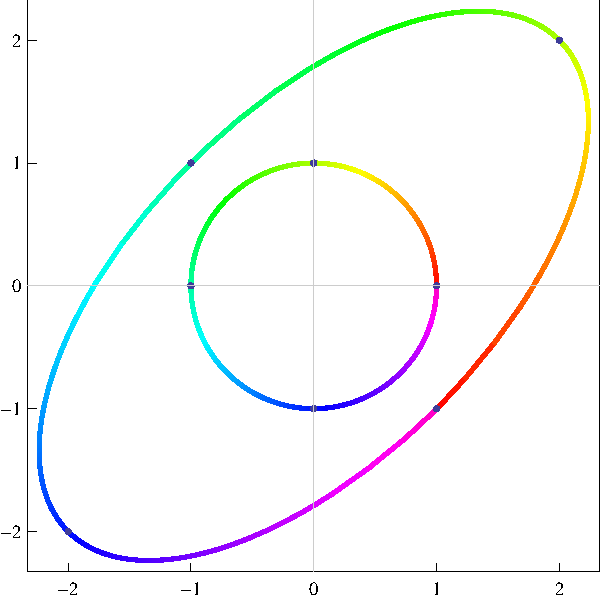
\includegraphics[ width = 2.5in ]{pdf/post_mortemII/dim_22_rank_2_image3} 
   \caption{The mapping action of the matrix in equation \eqref{eq:pmII:A} on all possible unit vectors in $\real{2}$. The coloring of the line is related to the angle. Fiducial marks are shown in increments of $\frac{\pi}{2}$.}
   \label{fig:maps:both}
\end{figure}

The next two plots, in figure \eqref{fig:maps:ev}, separate the curves and adds the eigenvectors. The black arrows are the first eigenvectors and the blue arrows are the second eigenvectors. The unit circle is resolved by the $\X{}$ matrix and the ellipse is resolved by the $\Y{}$ matrix \textit{scaled} by the singular values. This is codified in table \eqref{tab:pmII:blackblue}.

\begin{table}[htdp]
\begin{center}
\boxed{
\begin{tabular}{lrr}
  figure  & blue vector & black vector \\\hline
  circle  & $\X{}_{*,1}$\ \ \ \ \  & $\X{}_{*,2}$\ \ \ \ \  \\
  ellipse & $\sigma_{1} \Y{}_{*,1}$\ \ \ \ \  & $\sigma_{2} \Y{}_{*,2}$\ \ \ \ \ 
\end{tabular}
}
\end{center}
\label{tab:pmII:blackblue}
\caption{The eigenvectors of the domain and codomain and the scaling action of the eigenvectors.}
\end{table}%

This shows the vital relation between the column vectors of the domain and the scaled column vectors of the codomain:
\begin{equation}
  \A{} \X{}_{*,k} = \sigma_{k}\Y{}_{*,k}, \qquad k=1,\rho
  \label{eq:pmII:vital}
\end{equation}
This is of course just a rearrangement of the epitath
$$
\svdax{*}.
$$
The role of the singular values as scale factors is now clear after this demonstration. The blue vectors show the scaling effect of the first singular value; the black vectors the second singular value.

\begin{figure}[htbp] %  figure placement: here, top, bottom, or page
   \centering
   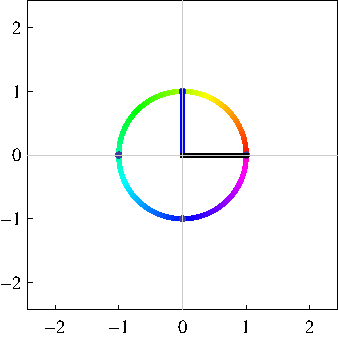
\includegraphics[ width = 2.25in ]{pdf/post_mortemII/circle_ev} \qquad
   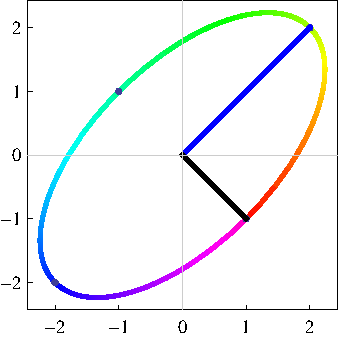
\includegraphics[ width = 2.25in ]{pdf/post_mortemII/ellipse_ev} 
   \caption{The pictorial demonstration of the scaling function of the singular values. The blue vectors show how $\A{} \X{}_{*,1} = \sigma_{k}\Y{}_{*,1}$ and the black vectors show $\A{} \X{}_{*,2} = \sigma_{2}\Y{}_{*,2}$.}
   \label{fig:maps:ev}
\end{figure}

%%
\subsection{The matrix in the simple method}
Look at the map in both directions

%%
\subsubsection{$\A{}x=y$}
\begin{figure}[htbp] %  figure placement: here, top, bottom, or page
   \centering
   \includegraphics[ ]{pdf/post_mortemII/toright} 
   \caption{Examine the mapping action of $\A{}$ from domain to codomain.}
   \label{fig:toright}
\end{figure}

The matrix described in equation \eqref{eq:simple:IamA}.
Recall the first decomposition \eqref{eq:simple:svd}
\begin{equation*}
  \begin{split}
    \svda{T} \\
    \Aexample &= \Yshade \Sigmaexampleb \Xtshade.
  \end{split}
\end{equation*}

Here the rank $\rho=1$ and so there is only one eigenvector to map. The eigenvector $\X{}_{*,1}$ maps to $\sigma_{1}\Y{}_{*,1}$. Since we can't distinctly see the mapping in the 3-dimensional image we show the explicit computation:
\begin{equation}
  \begin{split}
    \A{}\,\X{}_{*,1}\quad &= \quad \sigma_{1}\Y{}_{*,1}, \\
    \Aexample \frac{1}{\sqrt{2}}\mat{r}{1\\-1} \quad & =  \quad \sqrt{6}\frac{1}{\sqrt{3}}\mat{r}{1\\-1\\1}\\
    \frac{2}{\sqrt{2}}\mat{r}{1\\-1\\1}  \quad & =  \quad \sqrt{2}\mat{r}{1\\-1\\1}.
  \end{split}
\end{equation}

Herein lies the problem with the map. The dimension of the image, 1, is less than the dimension of the codomain, 3.

\begin{figure}[htbp] %  figure placement: here, top, bottom, or page
   \centering
   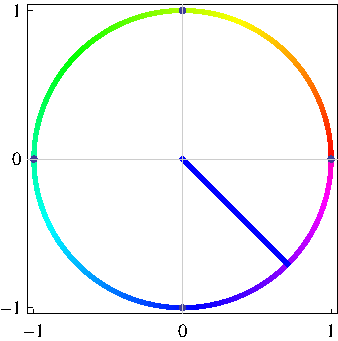
\includegraphics[ width = 1.9in ]{pdf/post_mortemII/a_circle_ev} \qquad
   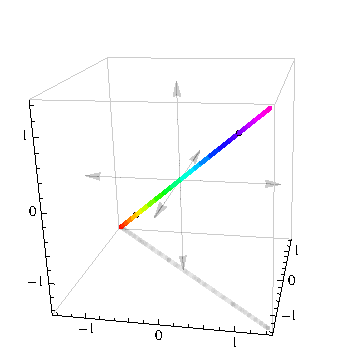
\includegraphics[ ]{pdf/post_mortemII/dim_32_rank_1_image} 
   \caption{The trouble with the matrix $\A{}$ (equation \eqref{eq:simple:IamA}) as a map from domain to codomain. The codomain has dimension 3 yet the image of the target matrix is a line with dimension 1. Because the line is embedded in a $3-$space a point on the line has three coordinates. But along the line there is only one coordinate measuring distance from the origin.}
   \label{fig:toright}
\end{figure}

%%
\subsubsection{$\A{T}y=x$}
\begin{figure}[htbp] %  figure placement: here, top, bottom, or page
   \centering
   \includegraphics[ ]{pdf/post_mortemII/toleft} 
   \caption{Examine the mapping action of the transpose matrix $\A{T}$ from codomain to domain.}
   \label{fig:toright}
\end{figure}
\begin{equation}
  \begin{split}
    \A{T} &= \svdt{T} \\
    \Atexample &= \Xshade \Sigmatexamplea \Ytshade.
  \end{split}
  \label{eq:simple:IamAT}
\end{equation}

\begin{equation}
  \begin{split}
    \A{}\,\X{}_{*,1}\quad &= \quad \sigma_{1}\Y{}_{*,1}, \\
    \Atexample \frac{1}{\sqrt{3}}\mat{r}{1\\-1\\1} \quad & =  \quad \sqrt{6}\frac{1}{\sqrt{2}}\mat{r}{1\\-1}\\
    \frac{3}{\sqrt{3}}\mat{r}{1\\-1}  \quad & =  \quad \sqrt{3}\mat{r}{1\\-1}.
  \end{split}
\end{equation}

\begin{figure}[htbp] %  figure placement: here, top, bottom, or page
   \centering
   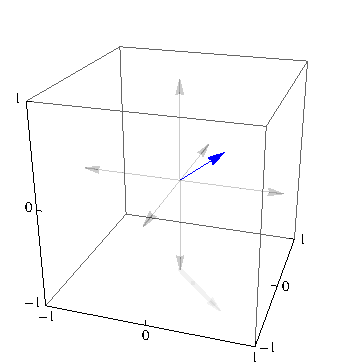
\includegraphics[ ]{pdf/post_mortemII/3_vector}  \qquad
   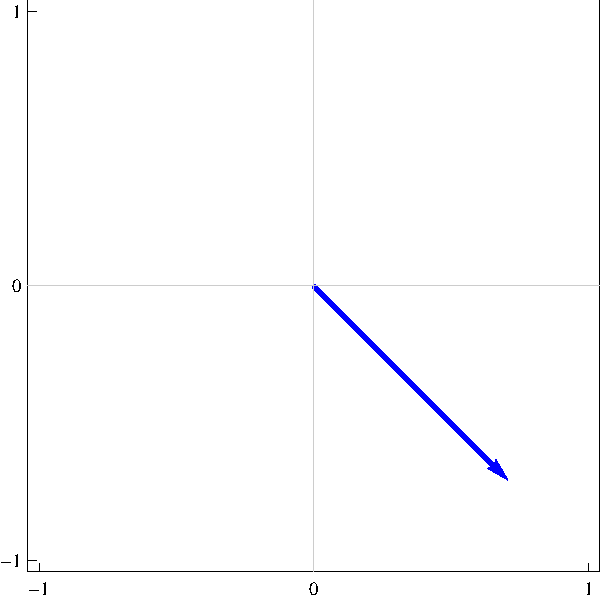
\includegraphics[ width = 1.9in ]{pdf/post_mortemII/430}
   \caption{The trouble with the matrix $\A{T}$ (equation \eqref{eq:simple:IamAT}) as a map from codomain to domain. The codomain has dimension 3 yet the image of the target matrix is a line with dimension 1. Because the line is embedded in a $2-$space a point on the line has two coordinates. But along the line there is only one coordinate measuring distance from the origin.}
   \label{fig:toleft}
\end{figure}

%%
\subsection{The matrix in the general method}
Look at the map in both directions

%%
\subsubsection{Domain $\longrightarrow$ cdomain}
\begin{figure}[htbp] %  figure placement: here, top, bottom, or page
   \centering
   \includegraphics[ ]{pdf/post_mortemII/toright} 
   \caption{Examine the mapping action of $\A{}$ from domain to codomain.}
   \label{fig:toright}
\end{figure}

Start with the first decomposition \eqref{eq:gen:soln}.
\begin{equation}
  \begin{split}
    \A{} &= \Y{}\paren{\sig{}\,\X{T}},\\
     &=
  \frac{1}{\sqrt{2}}
  \mat{rr}{1 & -1\\1 & 1}
  \frac{1}{\sqrt{2}}
  \paren{
  \mat{crc}
  {
  1 & 5  & 2 \\
  1 & -1 & 2
  }}, \\
  &=
  \mat{ccc}
  {
  0 & 3 & 0 \\
  1 & 2 & 2
  }.
  \end{split}
  \label{eq:gen:soln}
\end{equation}

Here the rank $\rho=1$ and so there is only one eigenvector to map. The eigenvector $\X{}_{*,1}$ maps to $\sigma_{1}\Y{}_{*,1}$. Since we can't distinctly see the mapping in the 3-dimensional image we show the explicit computation:
\begin{equation}
  \begin{split}
    \A{}\,\X{}_{*,1}\quad &= \quad \sigma_{1}\Y{}_{*,1}, \\
    \Aexample \frac{1}{\sqrt{2}}\mat{r}{1\\-1} \quad & =  \quad \sqrt{6}\frac{1}{\sqrt{3}}\mat{r}{1\\-1\\1}\\
    \frac{2}{\sqrt{2}}\mat{r}{1\\-1\\1}  \quad & =  \quad \sqrt{2}\mat{r}{1\\-1\\1}.
  \end{split}
\end{equation}

Herein lies the problem with the map. The dimension of the image, 1, is less than the dimension of the codomain, 3.

\begin{figure}[htbp] %  figure placement: here, top, bottom, or page
   \centering
   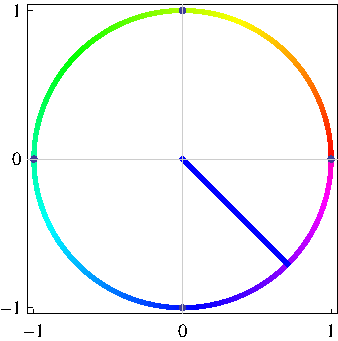
\includegraphics[ width = 1.9in ]{pdf/post_mortemII/a_circle_ev} \qquad
   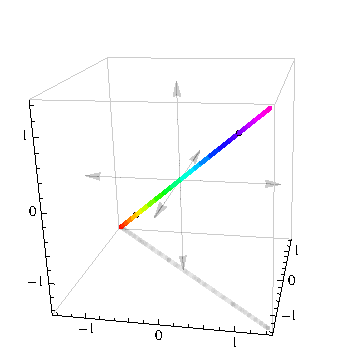
\includegraphics[ ]{pdf/post_mortemII/dim_32_rank_1_image} 
   \caption{The trouble with the matrix $\A{}$ (equation \eqref{eq:simple:IamA}) as a map from domain to codomain. The codomain has dimension 3 yet the image of the target matrix is a line with dimension 1. Because the line is embedded in a $3-$space a point on the line has three coordinates. But along the line there is only one coordinate measuring distance from the origin.}
   \label{fig:toright}
\end{figure}

%%
\subsubsection{$\A{T}y=x$}
\begin{figure}[htbp] %  figure placement: here, top, bottom, or page
   \centering
   \includegraphics[ ]{pdf/post_mortemII/toleft} 
   \caption{Examine the mapping action of the transpose matrix $\A{T}$ from codomain to domain.}
   \label{fig:toright}
\end{figure}
\begin{equation}
  \begin{split}
    \A{T} &= \svdt{T} \\
    \Atexample &= \Xshade \Sigmatexamplea \Ytshade.
  \end{split}
  \label{eq:simple:IamAT}
\end{equation}

\begin{equation}
  \begin{split}
    \A{}\,\X{}_{*,1}\quad &= \quad \sigma_{1}\Y{}_{*,1}, \\
    \Atexample \frac{1}{\sqrt{3}}\mat{r}{1\\-1\\1} \quad & =  \quad \sqrt{6}\,\frac{1}{\sqrt{2}}\mat{r}{1\\-1}\\
    \frac{3}{\sqrt{3}}\mat{r}{1\\-1}  \quad & =  \quad \sqrt{3}\mat{r}{1\\-1}.
  \end{split}
\end{equation}

\begin{figure}[htbp] %  figure placement: here, top, bottom, or page
   \centering
   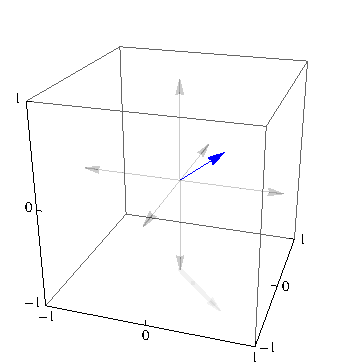
\includegraphics[ ]{pdf/post_mortemII/3_vector}  \qquad
   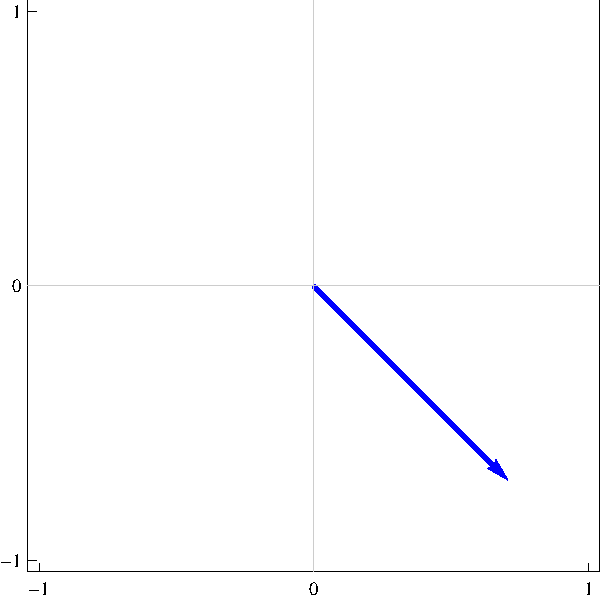
\includegraphics[ width = 1.9in ]{pdf/post_mortemII/430}
   \caption{The trouble with the matrix $\A{T}$ (equation \eqref{eq:simple:IamAT}) as a map from codomain to domain. The codomain has dimension 3 yet the image of the target matrix is a line with dimension 1. Because the line is embedded in a $2-$space a point on the line has two coordinates. But along the line there is only one coordinate measuring distance from the origin.}
   \label{fig:toleft}
\end{figure}


\endinput
\section{A survey of matrix mappings}
In the following pages we will look at three different kinds of mappings for a matrix $\Acc{m}{n}$: no frustration, frustration in one direction, frustration in both directions.

There are two different ways to view frustrated\index{frustration} mappings:
\begin{enumerate}
\item geometric deficiency\index{geometric deficiency} - mapping into a lower dimensional object;
\item algebraic deficiency\index{algebraic deficiency} - rank deficiency in row or column.
\end{enumerate}

In the examples that follow we will see ellipses mapped into other ellipses. These mappings are not frustrated. But once we map into a lower dimensional object, say from the unit sphere onto a line, the map is frustrated. This also means that we can't reverse the map. We can't make a finite linear map from a line with one parameter onto a sphere with three parameters.

These tables specify critical properties of the target matrix.

\textbf{Plots: }All plots start with the unit circle which is either
\begin{equation}
  \begin{array}{rcll}
     S(\theta) &=& \mat{c}{\cos \theta\\\sin \theta},\ \theta\in[0,2\pi) \qquad &n=2,\\
     S(\theta,\phi) &=& \mat{c}{\cos \theta\sin \phi\\\sin \theta \sin \phi\\\cos \phi},\ \theta\in[0,2\pi),\ \phi\in[0,\pi), \qquad &n=3.
  \end{array}
\end{equation}
Then look at the mapping action of the matrix. The result is either
\begin{equation}
  \A{}S(\theta) 
\end{equation}
when the target matrix has two columns or
\begin{equation}
  \A{}S(\theta,\phi) 
\end{equation}
when the target matrix has three columns.

The circles and ellipses have the color determined the the angular variable to provide an clearer idea of how the unit circle is distorted. So for the color red starts at $\theta=0$ and progresses through the spectrum until $\theta=2pi$ where the color is violet.\\

\textbf{Matrix images:} This block summarizes the plot above. For example, it may say that the plot represents a unit sphere being mapped to a line.\\

%%
\textbf{Vector space mappings:} These mappings are based on the dimensions of the spaces for the row and column vectors, $m$ and $n$. They disregard the issue of rank and and concerned purely with the mappings $\real{m}\mapsto\real{n}$ and  $\real{n}\mapsto\real{m}$. This map addresses the geometric deficiency of the mappings. For example are we going from a plane to a plane or a plane to a line. If the map is into a higher dimensional space we will have a frustrated map.\\

\textbf{Matrix ranks:} Are there rank deficiencies in the row or column space? If there is a rank deficiency we will see a frustrated map. 


\clearpage

%%
%% 2 x 2
%%
\begin{table}[htdp]
\begin{center}
\begin{tabular}{cc}
  $\A{}x=y$ & $\A{T}y=x$\\
 $\textellipsis$ & $\textellipsis$ \\
$\mat{rr}{1&2\\-1&2}\mat{c}{x_{1}\\x_{2}} = \mat{c}{y_{1}\\y_{2}}$ &
$\mat{rr}{1&-1\\2&2}\mat{c}{x_{1}\\x_{2}} = \mat{c}{y_{1}\\y_{2}}$ \\
\ \\
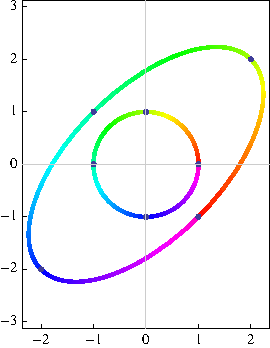
\includegraphics[ width = 2.15in ]{pdf/post_mortemII/2_2_2} &
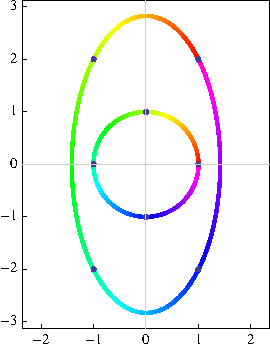
\includegraphics[ width = 2.15in ]{pdf/post_mortemII/2_2_2_t} \\
%%
\ \\
 matrix image & transpose matrix image \\
unit circle $\mapsto$ ellipse & unit circle $\mapsto$ ellipse\\
 $\textellipsis$ & $\textellipsis$ \\
vector space mappings & vector space mappings\\
(Domain) $\real{2} \mapsto \real{2}$ (Codomain) & (Codomain) $\real{2} \mapsto \real{2}$ (Domain)\\
 $\textellipsis$ & $\textellipsis$ \\
 full column rank  & full row rank\\
  $\textellipsis$ & $\textellipsis$ \\
 $\Ap=\AinvL$ & $\Ap=\AinvR$\\[10pt]
\end{tabular}
\end{center}
\label{tab:interpII:a}
\caption{Maps with no frustration. The domain and the codomain have the same dimension and the matrix has full rank. There are no null spaces associated with either the matrix or its transpose. The block dots are fiducial marks to help with comparing the orientation of the image (ellipse) relative to the target (circle). This matrix has full row rank, therefore the pseudoinverse is a left inverse. This matrix has full column rank, therefore the pseudoinverse is a right inverse. Because the pseudoinverse is both a left and a right inverse the pseudoinverse is also the standard inverse.}
\end{table}%

\clearpage
%%
%% 2 x 3
%%
\begin{table}[htdp]
\begin{center}
\begin{tabular}{cc}
  $\A{}x=y$ & $\A{T}y=x$\\
 $\textellipsis$ & $\textellipsis$ \\
$\mat{ccc}{0&3&0\\1&1&2}\mat{c}{x_{1}\\x_{2}\\x_{3}} = \mat{c}{y_{1}\\y_{2}}$ &
$\mat{cc}{0&1\\3&1\\0&2}\mat{c}{y_{1}\\y_{2}} = \mat{c}{x_{1}\\x_{2}\\x_{3}}$ \\
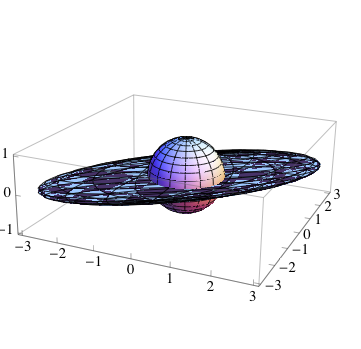
\includegraphics[ width = 2.5in ]{pdf/post_mortemII/3_2_2.png} &
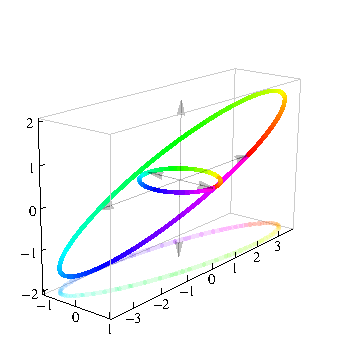
\includegraphics[ width = 2.5in ]{pdf/post_mortemII/3_2_2_t} \\
%%
vector space mappings & vector space mappings\\
(Domain) $\real{3} \mapsto \real{2}$ (Codomain) & (Codomain) $\real{2} \mapsto \real{3}$ (Domain)\\
 $\textellipsis$ & $\textellipsis$ \\
 matrix image & transpose matrix image \\
unit sphere $\mapsto$ elliptic disk & unit circle $\mapsto$ ellipse\\
 $\textellipsis$ & $\textellipsis$ \\
column rank deficient & full row rank\\
frustrated map\\
 $\textellipsis$ & $\textellipsis$ \\
 $\nexists\ \AinvL$ & $\Ap=\AinvR$\\[10pt]
\end{tabular}
\end{center}
\label{tab:interpII:a}
\caption{Frustration in one direction: domain to codomain. The frustration is signaled by the column rank deficiency where the matrix rank is less than the number of columns $(\rho<n)$. Notice that the mapping on the right is not frustrated; it is from a circle to an ellipse. Although both are two-dimensional objects, the ellipse is tipped and tilted out of the plane. The floor of the figure shows a shadow of the ellipse which helps to visualize the orientation in three-space. Because the matrix has full column rank the pseudoinverse is a right inverse.}
\end{table}

\clearpage
%%
%% 3 x 2
%%
\begin{table}[htdp]
\begin{center}
\begin{tabular}{cc}
  $\A{}x=y$ & $\A{T}y=x$\\
 $\textellipsis$ & $\textellipsis$ \\
$\Aexample \mat{c}{x_{1}\\x_{2}} = \mat{c}{y_{1}\\y_{2}\\y_{3}}$ &
$\Atexample\mat{c}{x_{1}\\x_{2}\\x_{3}} = \mat{c}{y_{1}\\y_{2}}$ \\
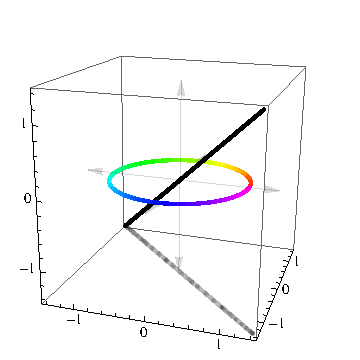
\includegraphics[ width = 2.5in ]{pdf/post_mortemII/3_2_1_a} &
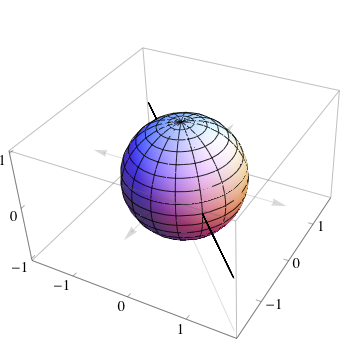
\includegraphics[ width = 2.5in ]{pdf/post_mortemII/3_2_1_t_a} \\
%%
vector space mappings & vector space mappings\\
(Domain) $\real{2} \mapsto \real{3}$ (Codomain) & (Codomain) $\real{3} \mapsto \real{2}$ (Domain)\\
 $\textellipsis$ & $\textellipsis$ \\
 matrix image & transpose matrix image \\
unit circle $\mapsto$ line & unit sphere $\mapsto$ line\\
 $\textellipsis$ & $\textellipsis$ \\
column rank deficient & row rank deficient\\
frustrated map & frustrated map\\
 $\textellipsis$ & $\textellipsis$ \\
 $\nexists\ \AinvL$ &  $\nexists\ \AinvR$ \\[10pt]
\end{tabular}
\end{center}
\label{tab:interpII:c}
\caption{Frustration in both directions, domain to codomain and back. The matrix rank is less than the number of rows $(\rho<m)$ and less than the number of columns $(\rho<n)$. The line is shown in black because the mapping is not one-to-one; multiple points in the target map to the same point in the image. Both figures show a projection of the image onto the floor of the figure. Because the matrix is both column and rank deficient there is neither a left nor a right inverse.}
\end{table}

\endinput



\endinput
\chapter{The domain matrices}
The domain matrices $\X{}$ and $\Y{}$ conjure considerable mystery. However under closer inspection we that they have elementary interpretations of unitary matrices. These domain matrices can be classified further as one of these types:
\begin{enumerate}
\item rotators
\item minimal spanning sets (bases)
\item reflections
\item permutations
\end{enumerate}

In the following sections we will discuss basic properties of unitary matrices then explore the different categories. 

The following chapters uses the Jordan normal form as a vehicle to probe these domain matrices.

Unitary matrices do not change the norm of a vector in $L_{2}$

Or course the product of unitary matrices are unitary.

\section{Unitary matrices}

Unitary matrices are easy to work with.
two views: a set of basis vectors, a process
unitary, orthogonal
\begin{equation}
  \U{}\U{*} = \I{}
\end{equation}
or
\begin{equation}
  \U{-1} = \U{*}
\end{equation}
Idempotent, index $k=2$.

Perhaps too much detail

spheres into spheres

%%
\subsection[Products of unitary matrices]{Products of unitary matrices are unitary}

An important realization is that the product of unitary matrices is also unitary. We will see that by looking at domain matrices as products of elementary unitary forms the \svdp \ looks much simpler.

Consider two conformable unitary matrices $\U{}\in\cmplx{m\times m}$ and $\V{}\in\cmplx{m\times m}$. Is there product unitary also?

Define
\begin{equation}
  \W{} = \U{}\V{*}.
\end{equation}
The question we are asking is this: Does the matrix product
\begin{equation}
  \W{}\W{}^{*} = \W{}^{*}\W{} = \I{m}?
  \label{eq:domains:unitarytest}
\end{equation}

To be explicit we show
\begin{equation}
  \W{}^{*}= \paren{\U{}\V{*}}^{*} = \paren{\V{*}}^{*}\U{*} = \V{}\U{*}.
\end{equation}
This implies the following:
\begin{equation}
  \begin{split}
    \W{}\W{}^{*} &= \paren{\U{}\V{*}}\paren{\V{}\U{*}}\\
      &=\U{} \paren{\V{*}\V{}} \U{*}\\
      &= \U{}\,\U{*}\\
      &= \I{m}.
  \end{split}
\end{equation}
A similar process shows that
\begin{equation}
  \W{}^{*}\W{} = \I{m}.
\end{equation}
Therefore the criteria of equation \eqref{eq:domains:unitarytest} are satisfied. Therefore the product of two unitary matrices is unitary. Therefore the product of three or more matrices are unitary.

This shows that a unitary matrix may be the composition of other unitary matrices. The implication is that we may examine the domain matrices and reveal a composition of elementary processes.

\endinput
\section{Planar coordinate systems}
Let's discuss orthogonal coordinate systems in the plane.

%%%
\subsection{Chirality in the plane}
\index{chirality!planar coordinate systems, of}
Recall the right-hand rule\index{right-hand rule} for an $x-y-z$ coordinate system. Start at the origin with your right hand and point your hand in the direction of increasing $x$. Curl your fingers in the direction of increasing $y$. Your thumb points in the direction of increasing $z$.

If your thumb points in the direction of decreasing $z$, then you have a left-handed coordinate system. What, you may ask, does this have to do with planar coordinate systems where $z=0$? We can use this concept to describe the \textit{orientation} of the coordinate system, as when we classify normal vectors\index{normal vectors} as inwards or outwards. If the planar coordinate system is right-handed, then we shade the object in green. For a left-handed system the shading is red. If we see a patch shaded green, the normal points towards us; red means the normal points away. ``Green is up'' and ``red is down.''

To illustrate these ideas we will start with the letter ``F'' in our reference coordinate system. When the letter is green it was plotted in a right-handed system. When the letter has other orientations in the plane, but is still green then we still have a right-handed coordinate system. When the forms of the letter are red, we are in a left handed coordinate system.


One way to approach this topic is to think of your computer screen as a blank slate for an orthogonal coordinate system. You may put the origin in any of the four corners. Once you have selected a corner anchor the coordinate system by serving as the origin, the next choice is pick the direction of increasing $x$. There are two choices for each corner. This is a total of eight different coordinate systems: four corner choices $\times$ two orientations per corner.

Let's pick one option as a reference and compare the others against it. Fix the origin in the lower left-hand corner and let the direction of increasing $x$ be along the horizontal to the right, much like when we draw a plot in the plane.

To facilitate the visualization, the $x-$axis is drawn in black, the $y-$axis in blue. Draw an angular arc from $x$ to $y$, from black to blue. If the angle is counterclockwise, the coordinate system is right-handed. Clockwise angles signal a left-handed coordinate system. This scheme is used in table \eqref{tab:chiral:rotations}.

\begin{table}[htdp]
\begin{center}
\begin{tabular}{cc}
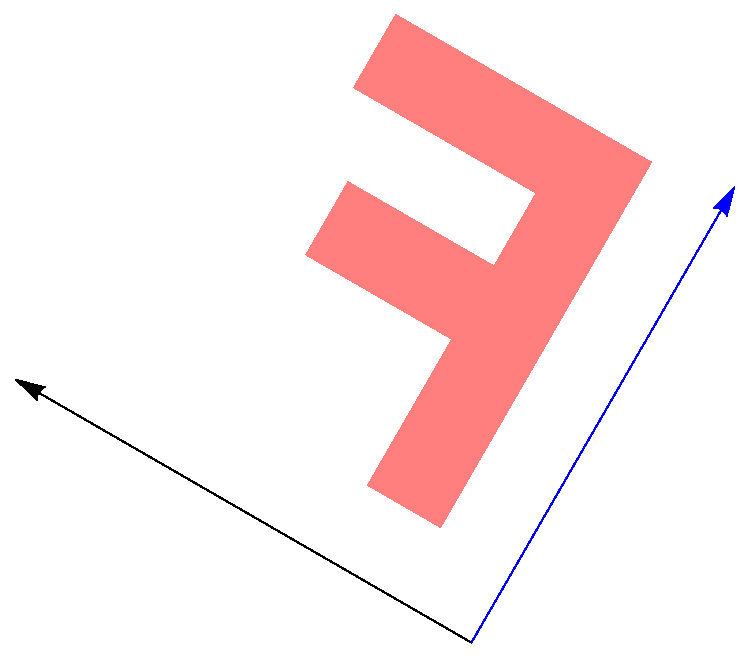
\includegraphics[ width = 2.25in ]{pdf/coordinate_systems/ref} &
\includegraphics[ width = 2.25in ]{pdf/coordinate_systems/rot} \\[10pt]
left-handed system & right-handed system\\[5pt]
 $\ktwo\mat{rr}{\cos \theta & -\sin \theta \\ \sin \theta & \cos \theta}\xtwo$ & 
 $\mat{rr}{\cos \theta & -\sin \theta \\ \sin \theta & \cos \theta}\xtwo$ \\[20pt]
\end{tabular}
\end{center}
\caption{Sample rotations in the plane. The $x-$axis is shown in black, the $y-$axis in blue. To jump between these images think of reflection through the line $y=x$. As you can imagine, such a reflection would require that the figure be turned over, revealing the other size.}
\label{tab:chiral:rotations}
\end{table}%

\begin{table}[htdp]
\begin{center}
\begin{tabular}{l|ll}
 & right-handed & left-handed   \\\hline
 patch color    & green   & red \\\hline
 patch surface  & top & bottom  \\\hline
 surface normal & outward & inward \\\hline
 angle: $x$ to $y$ & counterclockwise & clockwise \\\hline
\end{tabular}
\end{center}
\label{tab:chiral:youarerighthandedif}
\caption{Different ways to express the same concept.}
\end{table}%

\begin{table}[htdp]
\begin{center}
\begin{tabular}{m{1.75in}ll}
  \qquad image & \quad transformation & operation\\\hline
  \includegraphics[ width = 1.5in ]{pdf/coordinate_systems/Ia}   & $\itwo\xtwo=\mat{r}{x\\y}$ & identity\\\hline
  \includegraphics[ width = 1.5in ]{pdf/coordinate_systems/IIa}  & $\mat{rr}{0&1\\-1&0}\xtwo=\mat{r}{y\\-x}$ \qquad & rotation by $\pi/4$ \\\hline
  \includegraphics[ width = 1.5in ]{pdf/coordinate_systems/IIIa} & $\mat{rr}{-1&0\\0&-1}\xtwo=\mat{r}{-x\\-y}\qquad$ \qquad & rotation by $\pi/2$ \\\hline
  \includegraphics[ width = 1.5in ]{pdf/coordinate_systems/IVa}  & $\mat{rr}{0&-1\\1&0}\xtwo=\mat{r}{-y\\x}$ \qquad & rotation by $3\pi/4$ \\\hline
\end{tabular}
\end{center}
\label{tab:chiral:right}
\caption{Right-handed coordinate transformations. Think of the letter ``F'' as being composed of discrete points. The matrix operations show how each point is transformed in each of the images. Notice that in all cases the angular arc connecting the $x-$axis to the $y-$axis is $\pi/4$ counterclockwise.}
\end{table}%

\begin{table}[htdp]
\begin{center}
\begin{tabular}{m{1.75in}ll}
  \qquad image & \quad transformation & operation\\\hline
  \includegraphics[ width = 1.5in ]{pdf/coordinate_systems/Ib}   & $\mat{rr}{0&1\\1&0}\xtwo=\mat{r}{y\\x}$ & reflect through $y=x$\\\hline
  \includegraphics[ width = 1.5in ]{pdf/coordinate_systems/IIb}  & $\mat{rr}{0&1\\-1&0}\xtwo=\mat{r}{y\\-x}$ \qquad & rotation by $\pi/4$ \\\hline
  \includegraphics[ width = 1.5in ]{pdf/coordinate_systems/IIIb} & $\mat{rr}{-1&0\\0&-1}\xtwo=\mat{r}{-x\\-y}\qquad$ \qquad & rotation by $\pi/2$ \\\hline
  \includegraphics[ width = 1.5in ]{pdf/coordinate_systems/IVb}  & $\mat{rr}{0&-1\\1&0}\xtwo=\mat{r}{-y\\x}$ \qquad & rotation by $3\pi/4$ \\\hline
\end{tabular}
\end{center}
\label{tab:chiral:left}
\caption{Left-handed coordinate transformations.}
\end{table}%

\endinput
%\input{chapters/bases/rotators}
%\input{chapters/bases/reflectors}
%% fundamental projectors
\def\projra {\mathbf{P}_{\rng{\A{}}}}
\def\projrap{\mathbf{P}_{\rng{\A{}}^{\perp}}}
\def\projna {\mathbf{P}_{\nll{\A{}}}}
\def\projnap{\mathbf{P}_{\nll{\A{}}^{\perp}}}

\def\projrat {\mathbf{P}_{\rng{\A{T}}}}
\def\projratp{\mathbf{P}_{\rng{\A{T}}^{\perp}}}
\def\projnat {\mathbf{P}_{\nll{\A{T}}}}
\def\projnatp{\mathbf{P}_{\nll{\A{T}}^{\perp}}}

\providecommand{\aap}[1]   {\Y{}\,\sig{}\,\sig{(+)}\,\Y{#1}}
\providecommand{\apa}[1]   {\X{}\,\sig{(+)}\,\sig{}\,\X{#1}}

%\providecommand{\pra}[1]   {\Y{}\,\J{m}{\rho}\Y{#1}}
%\providecommand{\pnap}[1]  {\X{}\,\J{n}{\rho}\,\X{#1}}

\providecommand{\pra}[1]   {\yrng{}\yrng{#1}}
\providecommand{\pnap}[1]  {\xrng{}\xrng{#1}}

\endinput
%\input{chapters/bases/bases}
%\input{chapters/bases/GroupTheory}


\endinput
\chapter[Probing the SVD]{Probing the SVD with the Jordan normal form}
The Jordan normal forms offer a unique probe of the \svdp. These forms will act like an x-ray machine and show the internal structure  of the decomposition: permutations, rotations is stark relief. We will be able to correlate the most difficult decompositions to the more complete Jordan structures.

In \S \eqref{sec:Jordan:basic} we will see that the simpler Jordan forms have some of the basic non-trivial decompositions. These forms will cleanly show how the coordinate systems are rotated.

In \S \eqref{sec:Jordan:full} we will encounter the most daunting \svdl s: the full Jordan forms. The message will be clear that the difficulty with these decompositions lies in resolving trigonometric functions of angles $\zeta \pi$ where $\zeta$ is irrational.

In general, the \svdl \ of the Jordan normal forms fall into one of two categories: trivial or painful. This is an opportunity to put your pencil down and look at the patterns in the text.

\section[Basic Jordan forms]{The most basic Jordan forms}
\label{sec:Jordan:basic}

%%
\subsection{The forms}
There are seven nonzero, upper triangular $2\times2$ matrix Jordan forms and they are listed here:
\begin{equation*}
  \begin{array}{rclrclrcl}
\mathcal{J}_{2,1} &=& \left[
                        \begin{array}{cc}
                         1 & 0 \\
                         0 & 0
                        \end{array}
                        \right], \quad
\mathcal{J}_{2,2} &=& \left[
                        \begin{array}{cc}
                         0 & 1 \\
                         0 & 0
                        \end{array}
                        \right], \quad
\mathcal{J}_{2,3} &=& \left[
                        \begin{array}{cc}
                         1 & 1 \\
                         0 & 0
                        \end{array}
                        \right], \\
\mathcal{J}_{2,4} &=& \left[
                        \begin{array}{cc}
                         0 & 0 \\
                         0 & 1
                        \end{array}
                        \right], \quad
\mathcal{J}_{2,5} &=& \left[
                        \begin{array}{cc}
                         1 & 0 \\
                         0 & 1
                        \end{array}
                        \right], \quad
\mathcal{J}_{2,6} &=& \left[
                        \begin{array}{cc}
                         0 & 1 \\
                         0 & 1
                        \end{array}
                        \right], \\
\mathcal{J}_{2,7} &=& \left[
                        \begin{array}{cc}
                         1 & 1 \\
                         0 & 1
                        \end{array}
                        \right].
  \end{array}
\end{equation*}
The \svdl s are these:
\begin{equation}
  \begin{split}
\mathcal{J}_{2,1} &= 
\mat{cc}{ 1 & 0 \\
 0 & 0} = 
\I{2}
\mat{c|c}
{
 1 & 0 \\\hline
 0 & 0}
 \I{2}\\
\mathcal{J}_{2,2} &= 
\mat{cc}
{ 0 & 1 \\
 0 & 0} = 
\I{2}
\mat{c|c}{ 1 & 0 \\\hline
 0 & 0}
 \underbrace{\mat{cc}
 { 0 & 1 \\
\rowcolor{ltgray}
 1 & 0}}_{\text{swap rows}}\\
\mathcal{J}_{2,4} &= 
\mat{cc}
{ 0 & 0 \\
 0 & 1} = 
\underbrace{\mat{c>{\columncolor{ltgray}}c}
{ 0 & 1 \\
 1 & 0}}_{\text{swap columns}}
 \mat{c|c}
 { 1 & 0 \\\hline
 0 & 0}
 \underbrace{\mat{cc}
 { 0 & 1 \\
\rowcolor{ltgray}
 1 & 0}}_{\text{swap rows}}\\
\mathcal{J}_{2,5} &= 
\itwo
 = 
\I{2}\ 
\I{2}\ 
\I{2}
  \end{split}
\end{equation}
 
These nontrivial forms are related.
%%
\begin{equation*}
  \begin{array}{rcccccccc}
    \mathcal{J}_{2,3} &=& 
&\mat{cc}{ 1 & 1 \\
 0 & 0} 
 &=& 
&\I{2}
&\mat{c|c}
{\sqrt{2} & 0 \\\hline
 0 & 0}
& \stwo
\mat{rr}
{ 1 & 1 \\
\rowcolor{ltgray}
 -1 & 1},\\
    \mathcal{J}_{2,6} &=& 
&\mat{cc}
{0 & 1 \\
 0 & 1} 
 &=& 
& \stwo
\mat{r>{\columncolor{ltgray}}r}
{ 1 &-1 \\
  1 & 1}
&\mat{c|c}{
 \sqrt{2} & 0 \\\hline
 0 & 0}
&\I{2}.
  \end{array}
\end{equation*}

%%
\subsection{Example}
The two dimensional form of interest is this one:
\begin{equation}
  \begin{split}
    \mathcal{J}_{2,3} = \mat{cc}{1&1\\0&0} &= \svd{T}\\
      &= \I{2}\, \mat{c|c}{\sqrt{2} & 0\\\hline0 & 0} \stwo\mat{rr}{1&1\\\rowcolor{ltgray}
-1&1}.
  \end{split}
\end{equation}
This decomposition can also be written as a product of rotation matrices
\begin{equation}
  \begin{split}
    \mathcal{J}_{2,3} = \mat{cc}{1&1\\0&0} &= \svd{T}\\
      &= \rat{\theta_{y}}{}\, \mat{c|c}{\sqrt{2} & 0\\\hline
0 & 0} \rat{\theta_{x}}{T}
  \end{split}
\end{equation}
where the rotation matrix has this form
\begin{equation}
  \rat{\theta}{} = \mat{rr}{\cos\theta & -\sin\theta\\\sin\theta&\cos\theta}
\end{equation}
and the angles have these values
\begin{equation}
  \theta_{y} = 0, \quad \theta_{x} = \frac{\pi}{2}.
\end{equation}

The fact that the basis matrices are not unique manifests in the periodicity of the trigonometric functions. These rotation angles will also yield the same result:
\begin{equation}
  \theta_{y} = k\pi, \quad \theta_{x} = \frac{2k+1}{2}\pi, \quad k\in\mathbb{Z}.
\end{equation}
To emphasize this point the decomposition can be cast as this:
\begin{equation}
  \begin{split}
    \mathcal{J}_{2,3} = \mat{cc}{1&1\\0&0} = \svd{T} = \rat{k\pi}{}\mat{c|c}{\sqrt{2} & 0\\\hline0 & 0}\rat{\frac{2k+1}{2}\pi}{T},\quad k\in\mathbb{Z}. 
  \end{split}
\end{equation}
Noting the isomorphism between complex numbers and matrices of the form
\begin{equation}
  z = a + ib \quad \mapsto \quad \mat{cr}{a&-b\\b&a}, \quad a,b\in\real{}
\end{equation}
the decomposition can be written in this form
\begin{equation}
  \begin{split}
    \mathcal{J}_{2,3} = e^{i \theta_{y}}\mat{c|c}{\sqrt{2} & 0\\\hline0 & 0}e^{-i \theta_{x}}.
  \end{split}
\end{equation}

The transpose of this Jordan normal form 
\begin{equation}
    \mathcal{J}_{2,6} = \mathcal{J}_{2,3}^{\mathrm{T}}= \svd{T} 
    = e^{i\theta_{x}}\, \mat{c|c}{\sqrt{2} & 0\\\hline0 & 0} e^{-i\theta_{y}}
\end{equation}

\begin{equation}
  \chi \mat{c}{x\\y} = \mat{c}{y\\x}.
\end{equation}

\endinput
\section[Full Jordan forms]{The full $2\times2$ Jordan form}
\label{sec:Jordan:full}

The most vexations \svdl s involve the full Jordan forms. There are forms which are an entire upper triangular matrices of unit entries. If the target matrix is similar to a full Jordan form the \svdl \ will be arduous.

Consider the full form for the $2\times2$ Jordan forms. The depleted forms have trivial decompositions; the full form is much more complex.

\subsection{$2\times2$ form}
The full Jordan normal form for size $m=2$ and its decomposition is given by this
\begin{equation}
  \begin{split}
    \mathcal{J}_{2,7} = 
\mat{cc}{
 1 & 1 \\
 0 & 1
}
 &= \svd{T}\\
\Y{}&=\mat{rr}{
 \sqrt{\frac{1}{10} \left(5+\sqrt{5}\right)} & -\sqrt{\frac{1}{10} \left(5-\sqrt{5}\right)} \\
 \sqrt{\frac{1}{10} \left(5-\sqrt{5}\right)} & \sqrt{\frac{1}{10} \left(5+\sqrt{5}\right)}
}\\
\sig{}&=\mat{cc}{
 \frac{1}{2} \left(1+\sqrt{5}\right) & 0 \\
 0 & \frac{1}{2} \left(-1+\sqrt{5}\right)
}
\\
\X{}&=\mat{rr}{
 \sqrt{\frac{1}{10} \left(5-\sqrt{5}\right)} & -\sqrt{\frac{1}{10} \left(5+\sqrt{5}\right)} \\
 \sqrt{\frac{1}{10} \left(5+\sqrt{5}\right)} & \sqrt{\frac{1}{10} \left(5-\sqrt{5}\right)}
}.
  \end{split}
\end{equation}
%%%

This looks quite daunting until we see that we are dealing with rotator matrices using complementary angles:
%%%
\begin{equation}
  \begin{array}{ccccccc}
    \mathcal{J}_{2,7} &=& 
\mat{cc}
{
 1 & 1 \\
 0 & 1
}
 &=& \svd{T}\\
 &&&=& \rat{\theta}{}
&\mat{cc}{
 \alpha_{+} & 0 \\
 0 & \alpha_{-}
}
&\rat{\theta_{c}}{T}\\
 &&&=& e^{i\theta_{y}}
&\mat{cc}{
 \alpha_{+} & 0 \\
 0 & \alpha_{-}
}
&e^{-i\theta_{x}}
  \end{array}
\end{equation}
where the singular values are
\begin{equation}
  \alpha_{\pm} = \frac{1}{2} \left(\pm1+\sqrt{5}\right);
  \label{eq:j27:1}
\end{equation}
and the rotation angle is given by this
\begin{equation}
  \theta = \arcsin\paren{\sqrt{\frac{1}{10} \left(5-\sqrt{5}\right)}},
  \label{eq:j27:2}
\end{equation}
with $\theta_{c}$ being the complementary angle:
\begin{equation}
  \theta + \theta_{c} = \frac{\pi}{2}.
  \label{eq:j27:3}
\end{equation}


\endinput
\section[]{$3\times3$ Jordan forms}
\label{sec:Jordan:3}

In many cases $3\times3$ Jordan forms can be viewed as  block matrices with a $2\times2$ Jordan form and a zero matrix.

\subsection{Off-diagonal entries}
%%
Consider the forms where two off-diagonal entries are one.
\begin{equation}
  \begin{split}
    \mathcal{J}_{3,3} = 
\mat{ccc}
{
                1 & 1 & 0 \\
                0 & 0 & 0 \\
                0 & 0 & 0
}   &= \svd{T}\\
   &=
   %%  
\underbrace{\mat{c>{\columncolor{ltgray}}c>{\columncolor{ltgray}}c}
{
                1 & 0 & 0 \\
                0 & 0 & 1 \\
                0 & 1 & 0
}}_{\text{col 2 $\leftrightarrow$ col 3}}
%%
\mat{c|cc}{                
            \sqrt{2} & 0 & 0 \\\hline
            0 & 0 & 0 \\
            0 & 0 & 0
}%%  
\mat{rrr}
{                
\cos\theta & -\sin\theta & 0 \\
\rowcolor{ltgray}
0 & 0 & 1 \\
\rowcolor{ltgray}
\sin\theta & \cos\theta & 0
}
  \end{split}
\end{equation}
with
\begin{equation}
  \theta = -\frac{\pi}{4}.
\end{equation}
The $\X{}$ matrix represents a three dimensional coordinate system rotated by an angle $\theta$ about the line $x_{2}=x_{3}$. Only part of this rotation is ``visible''; the rest is ``hidden''in the null space.

The domain matrix $\X{}$ is a composition - or matrix product - of more fundamental orthogonal matrix forms. Any easy way to resolve this is to look at the action of the matrix upon an arbitrary vector:
\begin{equation}
 \mat{ccc}
{                
\cos\theta & -\sin\theta & 0 \\
0 & 0 & 1 \\
\sin\theta & \cos\theta & 0
} 
\mat{c}
{x\\y\\z}
=
\mat{c}
{x\cos\theta-y\sin\theta \\ z \\ x\sin\theta+y\cos\theta}
\end{equation}
We see these two operations:
\begin{enumerate}
\item a counterclockwise rotation of the $x-y$ axes by an angle $\theta$;
\item an interchange of the $y$ and $z$ axes.
\end{enumerate}
\begin{equation}
  \mat{ccc}
  {1&0&0\\
   0&0&1\\
   0&1&0}
  \mat{ccc}
  {\cos\theta & -\sin\theta & 0\\
   \sin\theta &  \cos\theta & 0\\
        0     &       0     & 1}
   =
\mat{ccc}
{                
\cos\theta & -\sin\theta & 0 \\
0 & 0 & 1 \\
\sin\theta & \cos\theta & 0
}
\end{equation}


%%%%%
Compare the related forms.
\begin{equation}
  \begin{split}
    \mathcal{J}_{3,5} = 
\mat{ccc}
{
                1 & 0 & 1 \\
                0 & 0 & 0 \\
                0 & 0 & 0
}   &= \svd{T}\\
   &=
   %%  
\underbrace{\mat{c>{\columncolor{ltgray}}c>{\columncolor{ltgray}}c}
{
                1 & 0 & 0 \\
                0 & 0 & 1 \\
                0 & 1 & 0
}}_{\text{col 2 $\leftrightarrow$ col 3}}
%%
\mat{c|cc}{                
            \sqrt{2} & 0 & 0 \\\hline
            0 & 0 & 0 \\
            0 & 0 & 0
}%%  
\mat{rcr}{                
                 \cos\theta & 0 & -\sin\theta \\
\rowcolor{ltgray}
                 \sin\theta & 0 &  \cos\theta \\
\rowcolor{ltgray}
                0 & 1 & 0
}
  \end{split}
\end{equation}
%%%
\begin{equation}
  \begin{split}
    \mathcal{J}_{3,6} = 
\mat{ccc}{
                0 & 1 & 1 \\
                0 & 0 & 0 \\
                0 & 0 & 0
}   &= \svd{T}\\
   &=
   %%  
\underbrace{\mat{c>{\columncolor{ltgray}}c>{\columncolor{ltgray}}c}
{
                1 & 0 & 0 \\
                0 & 0 & 1 \\
                0 & 1 & 0
}}_{\text{col 2 $\leftrightarrow$ col 3}}
%%
\mat{c|cc}{                
            \sqrt{2} & 0 & 0 \\\hline
            0 & 0 & 0 \\
            0 & 0 & 0
}%%  
\mat{rrr}{                
                0 & \cos\theta & -\sin\theta \\
\rowcolor{ltgray}
                0 & \sin\theta & \cos\theta \\
\rowcolor{ltgray}
                1 & 0 & 0
}
  \end{split}
\end{equation}

%%
\subsection{Embedding}
Embed the $\mathcal{J}_{2,7}$ block.
\begin{equation}
  \begin{split}
    \mathcal{J}_{3,11} &= 
\mat{cc|c}
{
                1 & 1 & 0 \\
                0 & 1 & 0 \\\hline
                0 & 0 & 0
}   = \svd{T}\\
   &=
   %%  
\mat{rr>{\columncolor{ltgray}}r}
{
                \cos\theta & -\sin\theta & 0 \\
                \sin\theta &  \cos\theta & 0 \\
                0 & 0 & 1
}
%%
\mat{cc|c}
{                
            \alpha_{+} & 0 & 0 \\
            0 & \alpha_{-} & 0 \\\hline
            0 & 0 & 0
}%%  
\mat{rrr}
{                
                 \cos\paren{-\theta_{c}} &  -\sin\paren{-\theta_{c}} & 0 \\
                 \sin\paren{-\theta_{c}} &   \cos\paren{-\theta_{c}} & 0 \\
\rowcolor{ltgray}
                0 & 0 & 1
}
  \end{split}
\end{equation}
where the singular values and angles have the same definitions as in equations \eqref{eq:j27:1}-\eqref{eq:j27:3}.

%%
\begin{equation}
  \begin{split}
    \mathcal{J}_{3,57} &= 
\mat{c|cc}
{
                0 & 0 & 0 \\\hline
                0 & 1 & 1 \\
                0 & 0 & 1
}   = \svd{T}\\
   &=
   %%  
\mat{rr>{\columncolor{ltgray}}r}
{
                0 & 1 & 0\\
                \cos\theta & 0 & -\sin\theta \\
                \sin\theta & 0 &  \cos\theta \\
}
%%
\mat{cc|c}
{                
            \alpha_{+} & 0 & 0 \\
            0 & \alpha_{-} & 0 \\\hline
            0 & 0 & 0
}%%  
\mat{rrr}
{                
                0 & \cos\paren{-\theta_{c}} & -\sin\paren{-\theta_{c}}\\
                1 & 0 & 0 \\
\rowcolor{ltgray}
                0 & \sin\paren{-\theta_{c}} & \cos\paren{-\theta_{c}} \\
}
  \end{split}
\end{equation}

There are three ways to embed this block in a $4\times4$ matrix.

%%
\begin{equation}
  \begin{split}
    \mathcal{J}_{4,19} &= 
\mat{cc|cc}
{
                1 & 1 & 0 & 0 \\
                0 & 1 & 0 & 0 \\\hline
                0 & 0 & 0 & 0 \\
                0 & 0 & 0 & 0
}   = \svd{T}\\
   &=
   %%  
\mat{cr>{\columncolor{ltgray}}c>{\columncolor{ltgray}}c}
{
                \cos\theta & -\sin\theta & 0 & 0 \\
                \sin\theta &  \cos\theta & 0 & 0 \\
                 0 & 0 & 0 & 1 \\
                 0 & 0 & 1 & 0 
}
%%
\mat{cc|cc}
{                
            \alpha_{+} & 0 & 0 & 0 \\
            0 & \alpha_{-} & 0 & 0 \\\hline
            0 & 0 & 0 & 0\\
            0 & 0 & 0 & 0
}%%  
\mat{ccrc}
{                
                0 & \cos\paren{-\theta_{c}} & -\sin\paren{-\theta_{c}} & 0 \\
                0 & \sin\paren{-\theta_{c}} &  \cos\paren{-\theta_{c}} & 0 \\
\rowcolor{ltgray}
                0 & 0 & 0 & 1 \\
\rowcolor{ltgray}
                1 & 0 & 0 & 0 \\
}
  \end{split}
\end{equation}
%%%
\begin{equation}
  \begin{split}
    \mathcal{J}_{4,176} &= 
\mat{c|cc|c}
{
                0 & 0 & 0 & 0 \\\hline
                0 & 1 & 1 & 0 \\
                0 & 0 & 1 & 0 \\\hline
                0 & 0 & 0 & 0 \\
}   = \svd{T}\\
   &=
   %%  
\mat{cr>{\columncolor{ltgray}}c>{\columncolor{ltgray}}c}
{
                 0 & 0 & 0 & 1 \\
                 \cos\theta & -\sin\theta & 0 & 0 \\
                 \sin\theta &  \cos\theta & 0 & 0 \\
                 0 & 0 & 1 & 0
}
%%
\mat{cc|cc}
{                
            \alpha_{+} & 0 & 0 & 0 \\
            0 & \alpha_{-} & 0 & 0 \\\hline
            0 & 0 & 0 & 0\\
            0 & 0 & 0 & 0
}%%  
\mat{ccrc}
{                
                0 & \cos\paren{-\theta_{c}} & -\sin\paren{-\theta_{c}} & 0 \\
                0 & \sin\paren{-\theta_{c}} &  \cos\paren{-\theta_{c}} & 0 \\
\rowcolor{ltgray}
                0 & 0 & 0 & 1 \\
\rowcolor{ltgray}
                1 & 0 & 0 & 0 \\
}
  \end{split}
\end{equation}
%%%
\begin{equation}
  \begin{split}
    \mathcal{J}_{4,896} &= 
\mat{cc|cc}
{
                0 & 0 & 0 & 0 \\
                0 & 0 & 0 & 0 \\\hline
                0 & 0 & 1 & 1 \\
                0 & 0 & 0 & 1
}   = \svd{T}\\
   &=
   %%  
\mat{cr>{\columncolor{ltgray}}r>{\columncolor{ltgray}}r}
{
                 0 & 0 & 0 & 1 \\
                 0 & 0 & 1 & 0 \\
                \cos\theta & -\sin\theta & 0 & 0 \\
                \sin\theta &  \cos\theta & 0 & 0
}
%%
\mat{cc|cc}
{                
            \alpha_{+} & 0 & 0 & 0 \\
            0 & \alpha_{-} & 0 & 0 \\\hline
            0 & 0 & 0 & 0\\
            0 & 0 & 0 & 0
}%%  
\mat{cccr}
{                
                0 & 0 & \cos\paren{-\theta_{c}} & -\sin\paren{-\theta_{c}} \\
                0 & 0 & \sin\paren{-\theta_{c}} &  \cos\paren{-\theta_{c}} \\
\rowcolor{ltgray}
                0 & 1 & 0 & 0 \\
\rowcolor{ltgray}
                1 & 0 & 0 & 0 \\
}
  \end{split}
\end{equation}
What happens when there are two blocks?
\begin{equation}
  \begin{split}
    \mathcal{J}_{4,915} &= 
\mat{cc|cc}
{
                1 & 1 & 0 & 0 \\
                0 & 1 & 0 & 0 \\\hline
                0 & 0 & 1 & 1 \\
                0 & 0 & 0 & 1
}   = \svd{T}\\
   \Y{} &=
   %%  
\mat{ccrr}
{
                 0 & \cos\theta & 0 & -\sin\theta \\
                 0 & \sin\theta & 0 & \cos\theta \\
                \cos\theta & 0 & -\sin\theta & 0 \\
                \sin\theta & 0 &  \cos\theta & 0
}\\
%%
\sig{} &=
\mat{cccc}
{                
            \alpha_{+} & 0 & 0 & 0 \\
            0 & \alpha_{+} & 0 & 0 \\\
            0 & 0 & \alpha_{-} & 0\\
            0 & 0 & 0 & \alpha_{-}
}\\
%%  
\X{T} &=
\mat{crcr}
{                
                0 & 0 & \cos\paren{-\theta_{c}} & -\sin\paren{-\theta_{c}} \\
                \cos\paren{-\theta_{c}} & -\sin\paren{-\theta_{c}} & 0 & 0 \\
                0 & 0 & \sin\paren{-\theta_{c}} &  \cos\paren{-\theta_{c}} \\
                \sin\paren{-\theta_{c}} &  \cos\paren{-\theta_{c}} & 0 & 0
}
  \end{split}
\end{equation}


\endinput

\endinput
\chapter[A More Formal Introduction]{A More Formal Introduction To The Singular Value Decomposition}
\label{chap:moreformal}

At this juncture we have reduced the \svdp \ to an operation which completes the induced row and column spaces to form unitary basis matrices connected by the matrix of singular values. This is the intuition we strive to edify by approaching the SVD from another perspective: the product matrix $\prdm{*}$.

\section{Every matrix has an SVD}

Part of the great utility of this transform comes from the fact that \textit{every} matrix has an SVD. Regardless of the shape of the matrix, regardless of its condition number, there will always be a SVD; it may not be unique, but it will exist.

Consider a matrix of rank $\rho$ such that $\Acc{m}{n}_{\rho}$. The singular value decomposition resolves $ \A{} $ into a product involving two unitary matrices $ \X{} $ and $ \Y{} $ and a diagonal-like matrix of the singular values $ \sig{} $. The decomposition is then
\begin{equation}
  \svdax{*}.
\end{equation}
Write out a table of matrix sizes to keep things sorted out:
$$
\boxed{
\begin{array}{ cllcc }
matrix & description & type & entries & dimension \\ \hline
 \A{}  & \text{target matrix} & \text{arbitrary} & \cmplx{} & m \times n \\[10pt]
 \Y{}  & \text{codomain basis} & \text{unitary} & \cmplx{} & m \times m \\
 \X{}  & \text{domain basis} & \text{unitary}& \cmplx{} & n \times n \\
 \sig{}& \text{singular values} & \text{diagonal-like} & \real{} & m \times n
\end{array}
}
$$

What does ``diagonal-like'' mean? In $ \sig{} $ there will be $ \rho $ non-zero entries and they will all be along the diagonal. For example, we could see forms like
\begin{equation}
  \mat{ccccc}
  {
  3 & 0 & 0 & 0 & 0\\
  0 & 3 & 0 & 0 & 0\\
  0 & 0 & 0 & 0 & 0\\
  }, \quad
  \mat{cc}
  {
  2 & 0\\
  0 & 1\\
  0 & 0\\
  }, \quad
  \mat{ccc}
  {
  \pi & 0           & 0\\
  0   & \sqrt[3]{2} & 0\\
  0   & 0           & \sqrt[4]{2}\\
  }.
\end{equation}

%%
\section{The SVD offers a simplified solution process}
\label{sec:formal:simple}
Now that have a definition of the SVD we turn to the question of its use. Given a \svdl, we can quickly solve linear systems $\ls$. The transforms go accordingly:
\begin{equation}
  \begin{array}{rcl}
  \A{}x &=& b \\
   &\Downarrow\\
   x &=& \A{+}b \\
   &\Downarrow\\
   x &=& \mpgi{*} b\\
   &\Downarrow\\
   \X{*} x &=& \sig{(+)}\Y{*} b
  \end{array}
\end{equation}
Introduce the \textit{change of coordinates}\index{change of coordinates} given by
\begin{equation}
  \begin{split}
    \mathbb{X} & = \X{*} x  \\
    \mathbb{B} & = \Y{*} b
    \label{eq:moreformal:a}
  \end{split}
\end{equation}
and we are left with a simpler linear system
\begin{equation}
    \mathbb{X} = \sig{(+)}\, \mathbb{B}.
    \label{eq:formal:svdsoln}
\end{equation}

While in general one would not turn to the SVD to solve a problem using least squares, the SVD is a powerful tool for theoretical studies. In this case, the SVD is used to transform a difficult problem to a simpler problem. Schematically,
$$
\begin{array}{ ccc }
  \A{} x = b  & \longrightarrow  &  \mathbb{X} = \sig{(+)}\, \mathbb{B} \\[5pt]
   \text{difficult}  & \longrightarrow  &  \text{simpler}  \\
\end{array}
$$
\textbf{Example:} 
For a demonstration take the target matrix and decomposition from the initial example in \eqref{eq:simple:problem}. The first coordinate transformation is this
\begin{equation}
  \begin{split}
    \mathbb{X} & = \X{T} x = \Xtshade \mat{c}{x_{1}\\x_{2}} = \stwo \mat{c}{x_{1}-x_{2}\\x_{1}+x_{2}}.
  \end{split}
\end{equation}
%%%
The second transformation is given by this:
\begin{equation}
  \begin{split}
    \mathbb{B} & = \Y{T} b \\
    &= \Ytshade \phivector \\
    &= \mat{r}{\sthree \\ \stwo \\ \frac{-2}{\sqrt{6}}}.
  \end{split}
  \label{eq:morefomal:B}
\end{equation}
%%%
The linear system is then reduced in the following steps:
\begin{equation}
  \begin{split}
    \mathbb{X} &= 
    \sig{(+)}\,\mathbb{B} \\
    \stwo 
    \mat{c}{x_{1}-x_{2}\\x_{1}+x_{2}} & = 
    \Sigmainverse
    \mat{r}{\sthree \\ \stwo \\ \frac{-2}{\sqrt{6}}}\\
    \stwo 
    \mat{c}{x_{1}-x_{2}\\x_{1}+x_{2}} &= 
    \mat{c}{\frac{1}{\sqrt{18}} \\ 0 \\ 0}.
  \end{split}
\end{equation}
These two lines have an interesting interpretation. The first line,
\begin{equation}
  x_{1} - x_{2} = \frac{1}{3}.
\label{eq:formal:2}
\end{equation}
describes the null space solution through the particular solution. The second line,
\begin{equation}
x_{2}=-x_{1}.
\label{eq:formal:1}
\end{equation}
describes the range or the row space\index{range!row space}.
From direct substitution of \eqref{eq:formal:1} into \eqref{eq:formal:2} we recover the point solution
\begin{equation}
  x_{1} = \rsix
\end{equation}
which with equation \eqref{eq:formal:1} leads to
\begin{equation}
  \mat{c}{x_{1} \\ x_{2}} = \frac{1}{6}\mat{r}{1\\-1},
\end{equation}
the particular solution as last seen in equation \eqref{eq:simple:fullsoln}.

%
%  Derivation of the SVD
%

\section{Derivation of the SVD}

We know what the SVD is and when to use it. Now we show how to derive the SVD. We begin not by looking at $\A{}$, but at the product matrix $\prdm{*}$  instead. While $\A{}$ has arbitrary shape, the product matrix  $\prdm{*}$  is square. And since this matrix is square we know it will have eigenvalues. The product matrix has three other essential properties.

%%
%%

\subsection{Three important properties}
\label{sec:moreformalbigthree}
The product matrix is defined as this
\begin{equation}
\begin{array}{ccc}
  \prdm{*} &=& \W{x},\\
  \paren{\byt{n}{m}}\paren{\byt{m}{n}} && \paren{\byt{n}{n}}.
\end{array}
\end{equation}
The matrix is square and its size is determined by the length of the \textit{row vectors}. These row vectors also determine the dimension of the domain. For this reason, the product matrix carries the \textit{x} subscript.

Besides being square, the product matrix also has three important properties. It is
\begin{enumerate}
  \item Hermitian,
  \item semi-positive definite, and
  \item normal.
\end{enumerate} 

Let's explore each of these properties more formally starting with the Hermiticity. 

%%%
%%%
%%%

\subsubsection{Hermitian}
Recall an Hermitian\index{Hermitian} matrix satisfies $ \B{} = \B{*} $. We see that the product matrix is automatically Hermitian since
\begin{equation}
  \paren{\prdm{*}}^{*}=\A{*}\paren{\A{*}}^{*} = \prdm{*}.
\end{equation}

Hermitian matrices are the backbone of Heisenberg's matrix version of quantum mechanics as they represent physical observables. These matrices have real eigenvalues as shown below.

To refresh, the Hermitian conjugate\index{Hermitian conjugate!definition} is the complex conjugate of the transpose matrix
\begin{equation*}
  \A{*} = \overline{\A{T}}.
\end{equation*}
(If the entries of the target matrix are all real then the complex conjugation does not change the entries.)

Start with a target matrix $\Acc{m}{n}_{\rho}$ and look at the eigenvalue equation for the target matrix $\A{}$ and the Hermitian conjugate of the equation:
\begin{equation}
\begin{split}
  \A{}x_{k} &= \lambda_{k}x_{k}, \quad k=1,\rho,\\
  \A{*}x^{*}_{k} &= \lambda^{*}_{k}x^{*}_{k}, \quad k=1,\rho.\\
\end{split}
\end{equation}
The difference between these equations is this
\begin{equation}
  \paren{\A{}-\A{*}} = \paren{\lambda_{k}-\lambda^{*}_{k}}\paren{2 \text{Re}\paren{x_{k}}}, \quad k=1,\rho.
\end{equation}
Because the target matrix is Hermitian the left hand side is zero and we have then
\begin{equation}
  \paren{\lambda_{k}-\lambda^{*}_{k}}\paren{2 \text{Re}\paren{x_{k}}}=0, \quad k=1,\rho.
\end{equation}
Because the vector $x$ is arbitrary it will not always have zero real part. Therefore the only way to enforce the zero product in all cases is to have
\begin{equation}
  \lambda_{k} = \lambda^{*}_{k}, \quad k=1,\rho.
\end{equation}
This is the requirement that all eigenvalues be real.

%%%
%%%
%%%

\subsubsection{Semi-positive definite}
A matrix $\A{}$ is semi-positive definite\index{semi-positive definite} if for all vectors $x$
\begin{equation}
  x^{*}\A{}x  \geq  0.
\end{equation}

Applying this to the product matrix $\prdm{*}$ we see
\begin{equation}
  x^{*}\prdm{*}x  \geq  0.
  \label{eq:formal:3}
\end{equation}

Using the eigenvalue equation $\A{}x=\lambda x$ we can rewrite equation \eqref{eq:formal:3} as
\begin{equation}
  x^{*}\prdm{*}x  =  \paren{\A{}x}^{*}\A{}x  =  \lambda^{*}\lambda = \abs{\lambda}^{2},
\end{equation}
clearly a positive number. Therefore the product matrix $\prdm{*}$ is semi-positive definite.

%%%
%%%
%%%

\subsubsection{Normal}

Lastly, we examine that it means for a matrix to be normal\index{normal matrix!definition}. A matrix $\A{}$ is normal when
\begin{equation}
  \prdm{*}  =  \prdmm{*}.
\end{equation}

Or in other terms, a normal matrix commutes with its Hermitian conjugate: 
\begin{equation}
  \brac{ \A{}, \A{*} } = \prdm{*}-\prdmm{*} =  0
\end{equation}
where the square brackets denote the commutator\index{commutator}.

How will this property help us? \textit{A normal matrix can be diagonalized by a unitary matrix.} That is, for $\B{}$ normal, there is a unitary matrix $\U{}$ such that the product matrix $\U{}\B{*}\U{*}$ is diagonal. In terms of the original product matrix $\prdm{*}$, we can state that $\U{}\prdm{*}\U{*}$ is diagonal. 

That is, if the matrix $\Ac{n}$ is normal then it satisfies
\begin{equation}
  \brac{ \A{}, \A{*} } = 0
\end{equation}
and there exits a unitary matrix
\begin{equation}
  \U{-1}  =  \U{*}
\end{equation}
such that the matrix product $\U{}\prdm{*}\U{*}$ is diagonal:
\begin{equation}
  \U{}\prdm{*}\U{*} = \mat{cccc}
  {
  \alpha_{1}\\
  &\alpha_{2}\\
  &&\ddots\\
  &&&\alpha_{n}\\
  }.
\end{equation}
The proof is left to other texts such !! as and !!.

%%
%%

\subsection{Construction of the SVD}

Let $ \lst{v_1, v_2, \cdots, v_n} $ be an orthonormal set of eigenvectors of the product matrix $\prdm{*}$ such that
\begin{equation}
  \prdm{*} v_j  =  \sigma_j^2 v_j.
\end{equation}

These $ \sigma $'s are the {\it singular values}. They are the non-zero {\it eigenvalues} of the square matrices $ \prdm{*} $ and $ \prdmm{*} $.

Here is an identity I wrote down. It looks important.
\begin{equation}
  \norm{ A v_j }_2^2 = v_j^* A^* A \sigma_j = v_j^* \sigma_j^2 v_j = \sigma_j^2
\end{equation}

Let the first $\rho$ singular values be greater than zero:
$$
\sigma_1, \sigma_2, \cdots, \sigma_\rho > 0;
$$

the remaining $p-\rho$ singular values are zero:

$$
\sigma_{\rho+1}, \sigma_{\rho+2}, \cdots, \sigma_p = 0
$$

where $\rho = \min \lst{m, n} $. This ensures that $ \A{} v_j = 0 $ if $ j > \rho $.

%
%
%
\section{Another example: SVD of block matrix}

The target matrix is
\begin{equation}
  \A{} = \frac{1}{10}\mat{crc}
  {
  0 &-8 & 3\\
  0 & 6 & 4\\
  0 & 0 & 0\\
  0 & 0 & 0\\
  }.
\end{equation}
We will be able to exploit a permutation matrix to solve this problem.

The first step is to form the product matrix
\begin{equation}
\begin{split}
  \W{x} = \prdm{T} &=  
  \mat{ccc}
  {
  0 & 0 & 0\\
  0 & 1 & 0\\
  0 & 0 & \frac{1}{4}\\
  }.
\end{split}
\end{equation}
For a diagonal matrix the eigenvalues are the diagonal entries. Therefore the eigenvalue spectrum of the product matrix is given by
\begin{equation}
  \lambda\paren{\W{x}} = \lst{0,1,\frac{1}{4}}.
\end{equation}
The singular values are the nonzero entries of the square-root of \textit{ordered} and \textit{truncated} list $\lambda'$:
\begin{equation}
  \sigma=\sqrt{\lambda'\paren{\W{x}}} = \sqrt{\lst{1,\frac{1}{4}}} = \lst{1,\frac{1}{2}}.
\end{equation}
\clearpage

%%%
%%%
\begin{xcb}{Exercises}
\begin{enumerate}
\item Show that the matrix product $\prdmm{*}$ is Hermitian.
\item Show that the matrix product $\prdmm{*}$ is semi-positive definite.
\item Consider the matrix $\Ac{m}{n}_{\rho}$. Describe the relationship between the eigenvectors of the matrix products $\prdm{*}$ and $\prdmm{*}$.
\subitem Answer: The matrices share the same $\rho$ non-zero eigenvalues. The product matrix $\W{x} = \prdm{*}$ will have $m-\rho$ zero-valued eigenvalues and the product matrix $\W{y} = \prdmm{*}$ will have $n-\rho$ zero-valued eigenvalues.
\item How do the singular values of the target matrix $\A{}$ relate to 
\subitem the eigenvalues of the product matrices, $\prdm{*}$ and $\prdmm{*}$?
\subitem Answer: the singular values are the the non-zero eigenvalues of the product matrices.
\subitem the eigenvalues of the target matrix $\A{}$? 
\subitem Answer: the singular values are the square-root of the non-zero eigenvalues of $\A{}$.
\end{enumerate}

\end{xcb}


\endinput

\part{Applications}
\chapter{Measuring the gradient}
Now that we have done some SVD's by hand we turn our attention to analytic computations using a software package such as \textit{Mathematica}. The results will be rewarding.

\section{The SVD in \textit{Mathematica}}

%%%
\subsection{Brevity}

%%%
\subsection{Intrinsic comands}

%%%
\subsection{SVD via QR decomposition}

%%%
\subsection{SVD via Householder reflection}

%%%
\subsection{SVD via Given rotations}


\endinput
\section{Direct calculation}

Consider the broad class of devices that measure the gradient of a scalar field. The idealization is this:
\begin{equation}
  \nabla \phi(x) = \psi(x), \qquad \phi, \psi \in L^{2}.
\end{equation}
The scalar field $\phi(x)3$ is the unknown object of interest and the vector field $\psi(x)$ is the known or measured field. The goal is to invert the equation and solve for $\phi(x)$ in terms of the data $\psi(x)$.

Over each measurement cell or interval of measurement the device registers a value $y_{k}$ corresponding to the average of the gradient of the scalar field over the cell.

Restrict the domain to the real line $\real{1}$, that is the scalar field
\begin{equation}
  \phi: \real{1}\to\real{1}.
\end{equation}
The measurement is the average of the gradient over a finite length,

%%
\subsection[The average of the gradient]{What is the average of the gradient?}
What do the data represent? In other words, what is the average of the gradient over an interval?

Consider the interval $I=[a,b]$ which has length $L=b-a$. The average of the gradient over this interval is defined formally as
\begin{equation}
  \overline{\nabla \phi}_{I} = \frac{\int_{a}^{b}{D_{x}\phi(x)dx}}{b-a}
\end{equation}
where $D_{x}$ represents the total differential operator in the $x$ variable. Using the Fundamental Theorem of Calculus\index{Fundamental Theorem of Calculus} this result is given by
\begin{equation}
  \overline{\nabla \phi}_{I} = \frac{\phi(b)-\phi(a)}{L}.
\end{equation}
The interpretation is basic: if we have knowledge of the average gradient across an interval we know about the \textit{difference} between the end points of the interval. Because we measure a derivative, we can only talk about differences between boundary points. For example the functions $\phi(x)$ and $\phi(x)+\alpha$ where $\alpha$ is an arbitrary constant, both have the same gradient and the same average gradient. That is
\begin{equation}
  \nabla \phi(x) = \nabla \paren{\phi(x)+\alpha}.
  \label{eq:gradient:invariance}
\end{equation}
This invariance will show up in the linear system as a rank deficiency.

There is even a broader class of equivalence. Since the average of the gradient just tells us about the difference between endpoint values, all functions which connect the endpoints are equivalent. An example is shown below. In each case the average of the gradient is zero.
\begin{figure}[htbp] %  figure placement: here, top, bottom, or page
   \centering
   \includegraphics[ width = 1.5in ]{pdf/gradient/gradient_1} \quad
   \includegraphics[ width = 1.5in ]{pdf/gradient/gradient_2} \quad
   \includegraphics[ width = 1.5in ]{pdf/gradient/gradient_3} 
   \caption{All three of the functions have the same average gradient since the boundary points have the same values. From a mathematical perspective, these functions are indistinguisable under the average gradient operator.}
   \label{fig:gradient:tres}
\end{figure}

Finally, it is convenient to work in cell space\index{cell space} where the length of each cell is identically one. In this case the average gradient over the $k$th cell becomes
\begin{equation}
  \overline{\nabla \phi}_{I_{k}} = \phi(k)-\phi(k-1) = \phi_{k} - \phi_{k-1}.
\end{equation}
Here the function arguments are replaced with integer subscripts tagging the $x$ location of the measurement. For example $\phi(0)$ becomes $\phi_{0}$.

%%
\section{Regularization}
The ambiguity expressed in equation \eqref{eq:gradient:invariance} reveals that we can't solve these problems directly. Just as in the first chapter the general solution has a nontrivial nullspace contribution. One way to think of the issue is to realize that we can't solve for $\Phi$, the values of the fields, instead we can only solve for differences between the field values.

Yet as in the first chapter, we can in fact compute a point solution; we can find a particular solution.  In this section we will regularize the linear system and create a problem with a direct solution. To do this we will introduce another constraint; in essence we will change the problem that we are solving. However, this will not change the particular solution.

We can learn a great deal by starting the simplest systems.  The single cell system demonstrates how the rank deficient system is solved by introducing another constraint. The double cell system which follows demonstrates how the need to arbitrate the vertices which are shared by two cells.

%%
\subsection{Single measurement cell}
Consider the simplest system: a single cell. There are two vertices, the endpoints on the left and right. The left vertex is at $x=0$ and the right vertex is at $x=1$. The cell spans the region between the vertices. The function values will be computed at the vertices and denoted by $\phi_{0}$ and $\phi_{1}$.

A convenient artifice is to represent the function values as sticks as shown in figure ???. We see the scalar field $\phi(x)$ over the sampling area of the cell. The actual field values are shown as $\phi_{0}$ and $\phi_{1}$. However the ideal device measures the average of the gradient which is the height difference $z_{1}$ between the $\phi_{0}$ and $\phi_{1}$. Mathematically the 
\begin{equation}
  \overline{\nabla\phi}_{I_{1}}=z_{1}=\phi_{1}-\phi_{0}.
\end{equation}
Notice that we are solving an idealization where we use the values of scalar field to describe the date. In an experiment the $z$ variables represent the measurements and the goal is to find the field values.

So given a measurement value of $z_{1}$ we only know that $\phi_{0}$ is $z_{1}$ units larger that $\phi_{1}$. What values do we assign to the field values then? The ambiguity takes this form
\begin{equation}
  \paren{\phi_{1}+\alpha}-\paren{\phi_{0}+\alpha}=z_{1}.
\end{equation}
In terms of a linear system we have this
\begin{equation}
  \begin{split}
    \A{}\Phi&=b\\
    \mat{cc}{-1&1}\mat{c}{\phi_{0}\\\phi_{1}}&=\brac{z_{1}}
    \label{eq:gradient:1d:system}
  \end{split}
\end{equation}
which does not offer a unique solution. There is a continuum of field values for the vertices of the form
\begin{equation}
  \phi_{1}=\phi_{0}+z_{1}.
\end{equation}
When we look at equation \eqref{eq:gradient:invariance} we see that the variable $\phi_{0}$ plays the role of the arbitrary constant $\alpha$.

How can we select a single solution? One may choose to fix the constant $\phi_{0} = 0.$ While this will work, this strategy does not extended to two and higher dimensions. Because devices of interest work in two and higher dimensions, we want to avoid this artifice.

To collapse the null space, we need another condition. A useful and natural choice is the \textit{zero sum condition}\index{zero sum condition}:
\begin{equation}
  \sum_{k=0}^{n}\phi_{k} = 0.
\end{equation}
In other words, just enforce the condition that the sum of the field measurements be zero.

With this condition we now have two equations with two unknowns:
\begin{equation}
  \begin{split}
    \phi_{0} + \phi_{1} &= 0.\\
    \phi_{1} - \phi_{0} &= z_{1}.
  \end{split}
\end{equation}
The linear system is then
\begin{equation}
  \begin{split}
    \A{} \Phi &= b\\
    \mat{rr}{1&1\\-1&1}\mat{c}{\phi_{0}\\\phi_{1}}&=\mat{c}{0\\z_{1}}.
  \end{split}
\end{equation}
The solution is given by this
\begin{equation}
  \begin{split}
    \Phi&=\A{-1}b\\
     \mat{c}{\phi_{0}\\\phi_{1}}&=\frac{1}{2}\mat{rr}{1&-1\\1&1}\mat{c}{0\\z_{1}}\\
     &=\frac{1}{2}\mat{r}{-z_{1}\\z_{1}}.
  \end{split}
  \label{eq:gradient:onecell:regular}
\end{equation}
The zero sum condition is manifest:
\begin{equation}
  \phi_{0}+\phi_{1}=-\frac{z_{1}}{2}+\frac{z_{1}}{2} = 0.
\end{equation}
Figure \eqref{fig:gradient:beforeafter} shows depictions of the incident scalar field on the left and the computation on the right. The solutions are equivalent modulo an additive constant.
\begin{figure}[htbp] %  figure placement: here, top, bottom, or page
   \centering
   \includegraphics[ width = 1in ]{pdf/gradient/Cauchy.jpg} 
   \caption{Before and after. The physical problem is on the left; the result of the computation is shown on the right.}
   \label{fig:gradient:beforeafter}
\end{figure}

%%
\subsection{Two measurement cells}
Consider the next simplest system: two cells sharing a vertex. The equations are these:
\begin{equation}
  \begin{split}
    \phi_{1}-\phi_{0}&=z_{1},\\
    \phi_{2}-\phi_{1}&=z_{2}.\\
  \end{split}
\end{equation}
The new wrinkle is that the shared vertex $\phi_{1}$ must satisfy two conditions. This represents the usual situation where we use a least squares fit to arbitrate these conflicting conditions.

We again have a rank deficient system reflecting the fact that we have two equations and three unknowns. The linear system is given by this:
\begin{equation}
  \begin{split}
    \A{}\Phi&=b,\\
    \mat{rrr}{-1&1&0\\0&-1&1}\mat{c}{\phi_{0}\\\phi_{1}\\\phi_{2}}&=\mat{c}{z_{1}\\z_{2}}.
  \end{split}
  \label{gradient:2:rd}
\end{equation}

Of course this system has a least squares solution. But before we turn to that in the next section, let's solve this problem by introducing the zero sum condition in the guise
\begin{equation}
  \phi_{0} + \phi_{1} + \phi_{2} = 0.
\end{equation}
Including this constraint with equation \eqref{gradient:2:rd} yields this
\begin{equation}
  \begin{split}
    \tilde{\A{}}\Phi&=b,\\
    \mat{rrr}{-1&1&0\\0&-1&1\\1&1&1}\mat{c}{\phi_{0}\\\phi_{1}\\\phi_{2}}&=\mat{c}{z_{1}\\z_{2}\\0}
  \end{split}
  \label{gradient:2:fr}
\end{equation}
which may be solved by elementary means. The solution is this
\begin{equation}
  \begin{split}
    \Phi &= \tilde{\mathbf{A}}^{-1}b\\
      \mat{c}{\phi_{0}\\\phi_{1}\\\phi_{2}}&=\frac{1}{3}\mat{rrr}{-2&-1&1\\1&-1&1\\1&2&1}\mat{c}{z_{1}\\z_{2}\\0}\\
      &= \frac{1}{3}\mat{r}{-2z_{1}-z_{2}\\z_{1}-z_{2}\\z_{1}+2z_{2}}.
  \end{split}
  \label{eq:gradient:2:reg}
\end{equation}

%%
\section{The least squares solution}
The pseudoinverse will have a new interpretation here.

%%
\subsection{Single measurement cell}
The system was described in equation \eqref{eq:gradient:1d:system}:
\begin{equation*}
  \begin{split}
    \A{}\Phi&=b\\
    \mat{cc}{-1&1}\mat{c}{\phi_{0}\\\phi_{1}}&=\brac{z_{1}}
  \end{split}
\end{equation*}

We can quickly recount the construction of least squares solution for the single cell. The product matrix is given by the outer product
\begin{equation}
  \begin{split}
    \W{x} & = \A{T}\A{} = \mat{r}{-1\\1}\mat{rr}{-1&1} = 
    \mat{rr}{1&-1\\-1&1}.
  \end{split}
\end{equation}

The characteristic polynomial $p(\lambda)$ is defined as this
\begin{equation}
  p(\lambda) = \det
  \mat{cc}{1-\lambda&-1\\-1&1-\lambda}.
\end{equation}
The eigenvalues are the zeros of the characteristic polynomial:
\begin{equation}
  p(\lambda) = \lambda^{2} - 2\lambda = 0.
\end{equation}
The two eigenvalues are these
\begin{equation}
  \lambda = \lst{2,0}.
\end{equation}
The singular values are the square root of the eigenvalues of the product matrix. Since the $\sig{}$ matrix has the same shape are the target matrix, we can write then that
\begin{equation}
  \sig{} = \mat{c|c}{\sqrt{2}&0}.
\end{equation}
The eigenvectors corresponding to the eigenvalues are these:
\begin{equation}
  v = \lst{\mat{r}{-1\\1},\mat{c}{1\\1}}.
\end{equation}
These domain matrix is assembled from the normalized versions of these vectors:
\begin{equation}
  \X{} = 
  \mat{c>{\columncolor{ltgray}}c}{\frac{v_{1}}{\normt{v_{1}}}&\frac{v_{2}}{\normt{v_{2}}}}
  = \stwo 
  \mat{r>{\columncolor{ltgray}}r}{-1&1\\1&1}.
\end{equation}
Because the target matrix $\A{}$ has rank $\rho=1$ there is only one vector in the range. The other vector must be in the null space.

By looking at the sizes of the component matrices, we see that the codomain matrix has size $1\times1$. The only possible normalized matrix is this
\begin{equation}
  \Y{} = \mat{c}{1}.
\end{equation}

The \svdl \ can now be assembled:
\begin{equation}
  \begin{split}
    \svda{T}\\
    \mat{cc}{-1&1} &=
    \mat{c}{1}
    \sqrt{2}\mat{c|c}{1&0}
    \stwo 
  \mat{rr}{-1&1\\\rowcolor{ltgray}1&1}.
  \end{split}
\end{equation}

The purpose of the decomposition was to construct the pseudoinverse:
\begin{equation}
  \begin{split}
    \mpgia{T}\\
    \rtwo\mat{r}{-1\\1} &=
    \stwo 
  \mat{r>{\columncolor{ltgray}}r}{-1&1\\1&1}
  \stwo
  \mat{c}{1\\\hline0}
  \mat{c}{1}.
  \end{split}
\end{equation}

The purpose of constructing the pseudoinverse was to compute the particular solution:
\begin{equation}
  \begin{split}
    \Phi_{p} &= \A{+}b\\
    \mat{c}{\phi_{0}\\\phi_{1}}_{p} &=
    \rtwo\mat{r}{-1\\1}
    \mat{c}{z_{1}}\\
    &=
    \rtwo\mat{r}{-z_{1}\\z_{1}}.
  \end{split}
\end{equation}
This is the same solution as found in equation \eqref{eq:gradient:onecell:regular} using regularization. 

As seen in equation \eqref{eq:simple:fullsoln}, the complete least squares solution is the particular solution plus the homogenous solution. The homogenous solution is revealed in the null vector in the domain matrix. Pulling these quantities together creates this expression:
\begin{equation}
  \begin{array}{rccccc}
    \Phi &=& \Phi_{p} &\oplus& \Phi_{h},\\[7pt]
      &=& \A{+}b &\oplus& \alpha \X{}_{*,2} , & \alpha \in \cmplx{}\\[7pt]
      &=& \rtwo\mat{r}{-z_{1}\\z_{1}} &\oplus& \alpha \mat{c}{1\\1}\\[17pt]
      &=& \textit{point} &\oplus& \textit{line}.
  \end{array}
\label{eq:simple:fullsoln}
\end{equation}
Here too we see two different topologies: the point form of the particular solution and the line corresponding to the homogenous solution.

The interpretation of the full least squares solution is straightforward. We see that the solution
\begin{equation}
  \Phi = \rtwo\mat{r}{-z_{1}\\z_{1}}
\end{equation}
is equivalent to this
\begin{equation}
  \Phi = \rtwo\mat{r}{-z_{1}+\alpha\\z_{1}+\alpha}, \quad \alpha \in \cmplx{}.
\end{equation}

Reflect upon this result. We obtained the same invariance condition as equation \eqref{eq:gradient:invariance} without knowing anything about the device. The least squares solution is a very powerful tool. Of course, the invariance condition manifest itself in construction of the linear system and in a sense the least squares solution merely recovered the invariance. But the \svdl \ has been powerful diagnostic instrument. 

%%
\subsection{Two measurement cells}
Let us apply the same least squares methodology to the device with two measurement cells. The linear system was posed in equation \eqref{gradient:2:rd}
\begin{equation*}
  \begin{split}
    \A{}\Phi&=b,\\
    \mat{rrr}{-1&1&0\\0&-1&1}\mat{c}{\phi_{0}\\\phi_{1}\\\phi_{2}}&=\mat{c}{z_{1}\\z_{2}}.
  \end{split}
\end{equation*}

For the purpose of providing another sample decomposition, we show the major milestones on the way to the SVD. The product matrix is this
\begin{equation}
  \W{x} = \A{T}\A{} =
  \mat{rrr}{-1&1&0\\0&-1&1}
  \mat{rr}{-1&0\\1&-1\\0&1} =
  \mat{rrr}{1&-1&0\\-1&2&-1\\0&-1&1}.
\end{equation}
The characteristic polynomial is then
\begin{equation}
  p(\lambda) = \paren{\lambda^{2}-4\lambda+3}(-\lambda).
\end{equation}
Therefore eigenvalue spectrum is given by this
\begin{equation}
  \lambda\paren{\W{x}} = \lst{3,1,0}.
\end{equation}
Therefore the $\sig{}$ matrix is this
\begin{equation}
  \sig{} = \mat{cc|c}{\sqrt{3}&0&0\\0&1&0}.
\end{equation}
The eigenvectors corresponding to the eigenvalues are these:
\begin{equation}
  v = \lst{
  \mat{r}{1\\-2\\1},
  \mat{r}{-1\\0\\1},
  \mat{r}{1\\2\\1}}.
\end{equation}
Therefore the domain matrix is this:
\begin{equation}
  \X{} = \mat{cc>{\columncolor{ltgray}}c}
  {\ssix & \frac{-1}{\sqrt{2}} & \sthree\\
   \frac{-2}{\sqrt{6}} & 0     & \sthree\\
   \ssix    & \stwo            & \sthree}
\end{equation}
The last column vector must be in the null space. The matrix $\A{}$ has rank $\rho=2$ and the first two vectors are in the image space.

Using the relationships
\begin{equation}
  \begin{split}
    \A{}\X{}_{*,1} &= \sigma_{1}\Y{}_{*,1},\\
    \A{}\X{}_{*,2} &= \sigma_{2}\Y{}_{*,2},
  \end{split}
\end{equation}
we solve for the two vectors in the codomain matrix $\Y{}$.

The \svdl \ of the system matrix $\A{}$ is this
\begin{equation}
  \begin{split}
    \svda{T}\\
    \mat{rrr}{-1&1&0\\0&-1&1}&=
    \stwo\mat{rr}{-1&1\\1&1}
    \mat{cc|c}{\sqrt{3}&0&0\\0&1&0}
    \mat{ccc}{
    \ssix&\frac{-2}{\sqrt{6}}&\ssix\\
    \frac{-1}{\sqrt{2}}&0&\stwo\\
    \rowcolor{ltgray}
     \sthree&\sthree&\sthree
    }.
  \end{split}
\end{equation}
The pseudoinverse is constructed as this:
\begin{equation}
  \begin{split}
    \mpgia{T}\\
    \frac{1}{3}
    \mat{rr}{-2&-1\\1&-1\\1&2} &=
    \mat{cc>{\columncolor{ltgray}}c}
   {\ssix & \frac{-1}{\sqrt{2}} & \sthree\\
    \frac{-2}{\sqrt{6}} & 0     & \sthree\\
    \ssix    & \stwo            & \sthree}
    \mat{cc}{\sthree &0\\0&1\\\hline0&0}    
    \stwo\mat{rr}{-1&1\\1&1}
  \end{split}
\end{equation}

The full least squares solution is the particular solution plus the homogeneous solution.  We repeat the presentation to stress the importance of the concept.
\begin{equation}
  \begin{array}{rccccc}
    \Phi &=& \Phi_{p} &\oplus& \Phi_{h},\\[7pt]
      &=& \A{+}b &\oplus& \alpha \X{}_{*,3} , & \alpha \in \cmplx{}\\
      &=& \rthree\mat{r}{-2z_{1}-z_{2}\\z_{1}-z_{2}\\z_{1}+2z_{2}} &\oplus& \alpha \mat{c}{1\\1\\1}\\[4pt]
      &=& \textit{point} &\oplus& \textit{line}
  \end{array}
\label{eq:simple:fullsoln}
\end{equation}
Again, the particular solution matches the solution via regularization, \eqref{eq:gradient:2:reg}

Notice that the particular solution satisfies the zero sum condition:
\begin{equation}
  \begin{array}{cccrcrcccccc}
     &\phi_{0}&=&-2z_{1}&-&z_{2}\\
    +&\phi_{1}&=&z_{1}&-&z_{2}\\
    +&\phi_{2}&=&z_{1}&+&2z_{2}\\\hline
     &\phi_{0}+\phi_{1}+\phi_{2}&=&&0
  \end{array}
\end{equation}

\endinput
\section{The least squares solution}

What solution do we get from the method of least squares? The decomposition of the system matrix is this
\begin{equation}
  \begin{split}
    \svda{T}\\
    \mat{rrr}{-1&1&0\\0&-1&1}&=
    \stwo\mat{rr}{-1&1\\1&1}
    \mat{cc|c}{\sqrt{3}&0&0\\0&1&0}
    \mat{rrr}{
    \ssix&-\frac{2}{\sqrt{6}}&\ssix\\
   -\stwo&0&\stwo\\
    \rowcolor{ltgray}
     \sthree&\sthree&\sthree
    }.
  \end{split}
\end{equation}
The pseudoinverse is constructed as this:
\begin{equation}
  \begin{split}
    \mpgia{T}\\
    \frac{1}{3}
    \mat{rr}{-2&-1\\1&-1\\1&2} &=
\left[
\begin{array}{rr>{\columncolor{ltgray}}r}
  \ssix & -\stwo & \sthree \\
 -\frac{2}{\sqrt{6}} & 0 & \sthree \\
  \ssix & \stwo & \sthree
\end{array}
\right]
    \mat{cc}{\sthree &0\\0&1\\\hline0&0}    
    \stwo\mat{rr}{-1&1\\1&1}
  \end{split}
\end{equation}
The shaded column represents the lone null space vector
\begin{equation}
  \mathcal{N} = \sthree \mat{c}{1\\1\\1}.
\end{equation}

The full least squares solution is the particular solution plus the homogenous solution:
\begin{equation}
\boxed{
  \begin{split}
    \Phi&=\A{\dagger}\Z{}+\beta\mathcal{N}\\
    \mat{c}{\phi_{0}\\\phi_{1}\\\phi_{2}}&=\frac{1}{3}
    \mat{rr}{-2&-1\\1&-1\\1&2}
    \mat{c}{z_{1}\\z_{2}}+\beta \mat{c}{1\\1\\1}, \quad \beta\in\cmplx{}.
  \end{split}
}
\end{equation}

Notice that the particular solution satisfies the zero sum condition:
\begin{equation}
  \begin{array}{cccrcrcccccc}
     &\phi_{0}&=&-2z_{1}&-&z_{3}\\
    +&\phi_{1}&=&z_{1}&-&z_{3}\\
    +&\phi_{2}&=&z_{1}&+&2z_{3}\\\hline
     &\phi_{0}+\phi_{1}+\phi_{2}&=&0
  \end{array}
\end{equation}


\endinput

\endinput
\chapter{Information and the singular values}
We can look at the singular values as a vessel for information about object


\section{The disk}

%%%
\subsection{Sharp edges}
\begin{table}[htdp]
\begin{center}
\begin{tabular}{cc}

\includegraphics[ width = 1.5in ]{pdf/fourier/disk_bw_0010}\\
\includegraphics[ width = 1.5in ]{pdf/fourier/disk_bw_0100}\\
\includegraphics[ width = 1.5in ]{pdf/fourier/disk_bw_1000}\\

\end{tabular}
\end{center}
\label{tab:fourier:disk}
\caption{default}
\end{table}%
\section{The disk}

%%%
\subsection{Softened edges edges}
\begin{table}[htdp]
\begin{center}
\begin{tabular}{cc}

\includegraphics[ width = 1.5in ]{pdf/fourier/dither_0003}\\
\includegraphics[ width = 1.5in ]{pdf/fourier/dither_0010}\\
\includegraphics[ width = 1.5in ]{pdf/fourier/dither_00100}\\
\includegraphics[ width = 1.5in ]{pdf/fourier/dither_00100}\\

\end{tabular}
\end{center}
\label{tab:fourier:dither}
\caption{default}
\end{table}%

\endinput

\endinput

\part{Formalities}
\chapter[The Fundamental Theorem]{The Fundamental Theorem of Linear Algebra}
At last we have arrived! The \ftola \ provides the organizing principles for the science of linear algebra. Often its erudition leaves practitioners feeling the subject is recondite and of secondary importance. The order and manner of presentation of the previous chapters show that we have tacked into this zephyr of ambivalence.

We see that the process of decomposition by singular values is simple in conception and often simple in execution. We see that the convenient perspective rests upon resolution of the row and vector spaces of the target matrix. This is just the Fundamental Theorem in thin disguise. The diagrams and tables are organized around the Fundamental Theorem. The facility of the simple SVD in the first chapter is due to the recognition of the Fundamental Theorem. Success to this point has come with the Fundamental Theorem lurking in the wings. It is time to call our star onto the stage, front and center.

%%
\section{The theorem}

There are several ways to state the theorem and the a few will be examined in the hope of providing perspective.

Every matrix induces two vector spaces: a row space and a column space.


\input{chapters/ftola/redos}
\section{Rank plus nullity}

This is a theorem we will use again and again.


\endinput
\section{The Fundamental Theorem in pictures}

\endinput

\endinput
\chapter[The SVD theorem]{The \svdl \ theorem}
Hopefully the statement of the \svdl \ theorem consolidates what we gave learned so far. The theorem itself is a collection of statements that should flow from memory. 


%%
\section{Theorem statement}

Given $\A{}\in\cmplx{\by{m}{n}}_{\rho}$, a complex matrix with $m$ rows and $n$ columns and rank $\rho$, where $\rho \le \min( m, n )$ then there exists a matrix decomposition of the format
\begin{equation}
  \svdax{*} .
\end{equation}
\begin{enumerate}
  \item The unitary matrix $\Y{}$ represents an orthonormal basis for the \textit{codomain}.
  \item The unitary matrix $\X{}$ represents an orthonormal basis for the \textit{domain}.
  \item There are $\rho$ positive \textit{singular values} which are the square roots of the nonzero eigenvalues of the product matrices $\prdm{*}$ and $\prdmm{*}$.
  \item The ordered singular values $\left( \sigma_1 \ge \sigma_2 \ge \cdots \ge \sigma_{\rho} > 0 \right)$ populate the diagonal $\textbf{S}$ matrix which is embedded in the $\sig{}$ matrix.
  \item The dimensions of associated matrices are shown here:
\begin{equation}
  \A{\byt{m}{n}}_{\rho} = 
  \Y{\byt{m}{m}}_{m}
  \mat{c|c}{
  \textbf{S}^{\by{\rho}{\rho}}_{\rho}  &  \zero \\\hline
  \zero  &  \zero
  }^{\by{m}{n}}_{\rho} 
  (\X{*})^{\by{n}{n}}_{n}.
\end{equation}
\end{enumerate}

%
\subsection{Important properties}
Thanks to the \index{Fundamental Theorem of linear algebra!dimensions for the SVD}Fundamental Theorem, the dimensions of the associated vector spaces are easily defined. Also, other important properties are evident.
\begin{enumerate}
\item The component matrices, $\sig{}$ and $\textbf{S}$ have the same rank $\rho$ as the target matrix.
\item In general the domain matrices are complex. The singular value matrix $\textbf{S}$ is always real. Therefore the sabot matrix $\sig{}$ which only pads the $\textbf{S}$ matrix with zero entries is always real.
\item The domain matrices $\Y{},\ \X{}$ along with the singular values matrix $\textbf{S}$ are square and invertible.
\item Because the domain matrices are unitary (orthogonal), the inverse matrix is the Hermitian conjugate (transpose).
\item Because the matrix of singular values is a full rank diagonal matrix, the matrix is square and the inverse matrix is has reciprocal values on the diagonal.
\item The sabot matrix $\sig{}$ has the same shape as the target matrix. This is a conformability bridge to allow the multiplication with the domain matrices.
\item The $\sig{}$ matrix is always unique.
\item The domain matrices are unique up to rotations or permutations.
\item Therefore, the \svdl \ is \textit{not} unique.
\item The nullity of the domain matrices is computed using the \index{rank plus nullity theorem:nullity of the domain matrices}rank plus nullity theorem. So while the domain matrices always have the same rank, they will have different nullities in general.
\subitem The nullity of the domain matrix is
\begin{equation}
  \eta_{x} = n - \rho.
\end{equation}
\subitem The nullity of the codomain matrix is
\begin{equation}
  \eta_{y} = m - \rho.
\end{equation}
\end{enumerate}

To reinforce these concepts we state the application of the rank plus nullity theorem to the $n-$dimensional vector space of the domain and the $m-$dimensional vector space of the codomain
\begin{equation}
\boxed{
  \begin{array}{rcllclclcl}
    \text{rank } \rng{\A{}} &+& \text{nullity } \nll{\A{}} & = & \rho + \eta_{x} & = & \rho + (n-\rho) & = & n,\\
    \text{rank } \rng{\A{*}} &+& \text{nullity } \nll{\A{*}} & = & \rho + \eta_{y} & = & \rho + (m-\rho) & = & m.
  \end{array}
}
\end{equation}
As basic as it seems it is still something users stumble over.

In terms of matrix rank, a rank deficient matrix is resolved into a product of a full rank matrix with a rank deficient matrix with another full rank matrix.

%
\subsection{Unimportant properties}
The SVD is bound by convention. One could develop an equivalent theorem based upon the formulation
\begin{equation}
  \A{} = \Y{*}\,\sig{}\,\X{}.
\end{equation}
In other words, we could move the Hermitian conjugation to the other side.

Also, as mentioned before, we could allow the singular values to be left unsorted. Keeping them arranged in descending order is a good housekeeping practice which makes applications cleaner and easier to formulate.

Some authors allow the singular values to be zero. The first $\rho$ values are nonzero, and the last $min(m,n)-\rho$ values are zeros. Again, it is a preference which could be accounted for by modest rewording of applications.

One way to state the theorem may be a bit preferable to some readers. We can write equivalently that
\begin{equation}
  \Y{*}\,\A{}\,\X{} = \sig{}.
\end{equation}
Fans of diagonalization may champion this form.

%%
\section{Four fundamental subspaces}
The \svdl \ resolves a matrix into its four fundamental subspaces:
\begin{enumerate}
\item Codomain: the range of the target matrix, $\rng{\A{}}$,
\item Codomain: the null space of the Hermitian conjugate of target matrix,  $\nll{\A{*}}$,
\item Domain: the range of the Hermitian conjugate of the target matrix, $\rng{\A{*}}$,
\item Domain: the null space of the target matrix,  $\nll{\A{}}$,
\end{enumerate}

The figure below shows how the vectors are represented in the decomposition.
\begin{enumerate}
\item First $\rho$ columns of $\Y{}$: $\rng{\A{}}$.
\item Last $m-\rho$ columns of $\Y{}$: $\nll{\A{*}}$.
\item First $\rho$ rows of $\X{*}$: $\rng{\A{*}}$.
\item Last $n-\rho$ rows of $\X{}$: $\nll{\A{}}$.
\end{enumerate}

Big four in pictures. Pedro's diagram.


%%
\section{Dimension and size}
\index{size!matrix}\index{dimension!vector space}
The size of a matrix describes the number of rows and columns. The dimension of  a vector space describes the length of the constituent vectors.

%%
\section{The spectral theorem and SVD}
We know from linear algebra that a symmetric matrix can be diagonalized by a unitary matrix. So given a matrix
\begin{equation}
  \lst{\W{} \in \cmplx{\bys{m}}_{m}\colon\mathbf{W}_{r,c}=\mathbf{W}_{c,r}, r,c=1\dots m}
\end{equation}
there exists a unitary matrix $\Q{}$ such that the matrix $\Lambda$ is diagonal.
\begin{equation}
  \W{} = \Q{}\,\Lambda\,\Q{*}.
\end{equation}

\begin{equation}
  \begin{split}
    \W{x} = \prdm{*} &= \paren{\svdt{*}}\paren{\svd{*}} \\
    &= \X{}\,\sig{T}\sig{}\,\X{*}.
  \end{split}
\end{equation}
\begin{equation}
  \begin{split}
    \W{y} = \prdmm{*} &= \paren{\svd{*}}\paren{\svdt{*}}\\
    & = \vy{*}.
  \end{split}
\end{equation}In terms of the spectral theorem, the product matrices can be decomposed into similarity transform where $\Lambda$ is a diagonal matrix of eigenvalues and the matrix $\Q{}$ is unitary.
\begin{equation}
  \begin{split}
    \W{x} &= \vx{*}\\
          &= \Q{}\,\Lambda\,\Q{*}.
  \end{split}
\end{equation}

\begin{equation}
  \W{x} = \mat{c}{r_{1}\\r_{2}\\\vdots\\r_{n}} \mat{c}{\sigma_{1}r_{1}^{\mathrm{T}}}
\end{equation}


\endinput
\section[Special types]{The SVD for special types of matrices}
We can boost intuition by studying the decomposition of special matrix types.

%%%
\subsection{Normal matrices}
\begin{equation}
  \brac{\A{},\A{*}} = \prdmm{*} - \prdm{*} = 0.
\end{equation}

%%%
\subsection{Idempotent matrices}
\begin{equation}
  \A{2} = 0.
\end{equation}
\begin{equation}
  \A{k} = 0.
\end{equation}

%%%
\subsection{Nilpotent matrices}
\begin{equation}
  \A{2} = \zero.
\end{equation}
\begin{equation}
  \A{k} = \zero.
\end{equation}

%%%
\subsection{Symmetric matrices}
\begin{equation}
  \A{} = \A{T}.
\end{equation}

%%%
\subsection{Hermitian matrices}
\begin{equation}
  \A{} = \A{*}
\end{equation}

%%%
\subsection{SPD matrices}
\begin{equation}
  z^{\mathrm{T}}\A{}z \ge 0
\end{equation}

%%%
\subsection{Diagonally dominant matrices}


\endinput
\section{The product matrices and orthogonal expansions}

The product matrices $\W{x}$ and $\W{y}$ offer important insights to the SVD.

%%
\subsection{Theory}
The outer products express the orthogonality of the expansion. For example
\begin{equation}
  \begin{split}
    \W{x} = \prdm{*} = \paren{\sum_{k=1}^{\rho}{\sigma_{k}\, \Y{}_{k}\, \X{*}_{k}}}^{*}\sum_{j=1}^{\rho}{\sigma_{j}\, \X{}_{j}\, \Y{*}_{j}}.
  \end{split}
\end{equation}
The orthogonality condition flows naturally from the unitary nature of the domain matrices:
\begin{equation}
  \X{*}_{k}\,\X{}_{j} = \Y{*}_{k}\,\Y{}_{j} =
  \begin{cases}
    1 & k = j\\
    0 & k \ne j
  \end{cases}.
\end{equation}

The cross terms with $k\ne j$ vanish:
\begin{equation}
  \begin{split}
    \paren{\sigma_{j}\, \Y{}_{j}\, \X{*}_{j}}^{*}\paren{\sigma_{k}\, \Y{}_{k}\, \X{*}_{k}} &= \paren{\sigma_{j}\X{}_{j}\, \Y{*}_{j}}\paren{\sigma_{k}\Y{}_{k}\, \X{*}_{k}}, \\
    &= \sigma_{k}\sigma_{j}\X{}_{k}\underbrace{\paren{\Y{*}_{k}\,\Y{}_{j}}}_{0}\X{*}_{j}\\
    & = \zero,
  \end{split}
\end{equation}
an $m\times m$ matrix of zeros.

The cross terms with $k=j$ are the survivors:
\begin{equation}
  \begin{split}
    \paren{\sigma_{k}\, \Y{}_{k}\, \X{*}_{k}}^{*}\paren{\sigma_{k}\, \Y{}_{k}\, \X{*}_{k}}&= \paren{\sigma_{k}\X{}_{k}\, \Y{*}_{k}}\paren{\sigma_{k}\Y{}_{k}\, \X{*}_{k}} \\
    &= \sigma_{k}^{2}\,\X{}_{k}\paren{\Y{*}_{k}\,\Y{}_{k}}\X{*}_{k}\\
    &= \sigma_{k}^{2}\,\prodx{*}{k}.
  \end{split}
\end{equation}

The final result is this
\begin{equation}
  \W{x} = \prdm{*} = \sum_{k=1}^{\rho}{\sigma_{k}^{2}\,\prodx{*}{k}}.
\end{equation}
By similar machinations we find the complementary product matrix
\begin{equation}
  \W{y} = \prdmm{*} = \sum_{k=1}^{\rho}{\sigma_{k}^{2}\,\prody{*}{k}}.
\end{equation}
Notice the similarity of this formulation to the expression using the full matrices.

In terms of the \svdl \ the product matrices are these
\begin{equation}
  \begin{array}{rccccccl}
    \W{x} &=& \prdm{*}  &=& \paren{\svd{*}}^{*}&\svd{*} &=& \wx{*},\\
    \W{y} &=& \prdmm{*} &=& \svd{*}&\paren{\svd{*}}^{*} &=& \wy{*}.
  \end{array}
\end{equation}

Compare the equivalent formulations to see the stenciling and shape arbitration effects of the $\sig{}$ matrix. The matrix formulation shows the stenciling action of the $\sig{}$ matrix. The second expression is a sum of outer products scaled by the squares of the singular values:
\begin{equation}
  \begin{array}{rcccc}
    \W{x} &=& \wx{*} &=& \sum_{k=1}^{\rho}{\sigma_{k}^{2}\,\prodx{*}{k}},\\[10pt]
    \W{y} &=& \wy{*} &=& \sum_{k=1}^{\rho}{\sigma_{k}^{2}\,\prody{*}{k}}.
  \end{array}
\end{equation}
The Fourier-Bessel expansion represents the thin SVD\index{thin SVD}; the null space vectors are never encountered.

%%
\subsection{Examples}
Let's go back through some earlier examples and show the details explicitly. 

%%
\subsubsection{Canonical example: $\by{3}{2}$, rank $\rho=1$}
Begin with equation \eqref{eq:simple:svd}:

\begin{equation*}
\begin{split}
    \svda{T}\\
    \archetypez.
\end{split}
\end{equation*}

The product matrices are these:
\begin{equation}
  \begin{array}{lccc}
     \W{x} = \prdm{T}  =& \Atexample  \Aexample   &=& 3 \mat{rr}{1&-1\\-1&1},\\
     \W{y} = \prdmm{T} =& \Aexample   \Atexample  &=& 2 \mat{rrr}{1&-1&1\\-1&1&-1\\1&-1&1}.\\
  \end{array}
\end{equation}

In terms of an outer product expansion the product matrices are assembled in this fashion:
\begin{equation}
  \begin{array}{lcc}
     \W{x} = \sigma^{2}\, \prodx{T}{1} = 6\, \stwo   \mat{r}{1\\-1}   \stwo \mat{rr}{1&-1}     =& 3 \mat{rr}{1&-1\\-1&1},\\[5pt]
     \W{y} = \sigma^{2}\, \prody{T}{1} = 6\, \sthree \mat{r}{1\\-1\\1}\sthree\mat{rrr}{1&-1&1} =& 2 \mat{rrr}{1&-1&1\\-1&1&-1\\1&-1&1}.
  \end{array}
\end{equation}

%%%
%%%
\subsubsection{Increase the matrix rank: $\by{2}{3}$, rank $\rho=2$}
Begin with equation \eqref{eq:general:ysxt}:
\begin{equation*}
  \begin{array}{ccccc}
    \A{} &=& \Y{} & \sig{} & \X{T}\\
  \mat{ccc}
  {
  0 & 3 & 0 \\
  1 & 2 & 2
  } 
  &=&
  \frac{1}{\sqrt{2}}
  \mat{rr}{1 & -1\\1 & 1}
  &
  \mat{cc|c}
  {
  \sqrt{15} & 0 & 0 \\
  0 & \sqrt{3}  & 0
  }
  &
  \mat{ crr }
 {\frac{1}{\sqrt{30}} & \frac{5}{\sqrt{30}} & \frac{2}{\sqrt{30}}\\
  \rsix               & \frac{-1}{\sqrt{6}} & \frac{2}{\sqrt{6}} \\
  \rowcolor{ltgray}
  \frac{-2}{\sqrt{5}} & 0                   & \frac{1}{\sqrt{5}}}\\[25pt]
  \end{array}.
\end{equation*}

The product matrices are these:
\begin{equation}
  \begin{array}{lccc}
     \W{x} = \prdm{T}  =& 
  \mat{ccc}
  { 0 & 1 \\
    3 & 2 \\
    0 & 2
  }  
  \mat{ccc}
  {
  0 & 3 & 0 \\
  1 & 2 & 2
  } 
     &=& 
  \mat{ccc}
  {
  1 &  2 & 2 \\
  2 & 13 & 4 \\
  2 &  4 & 4 
  },\\
     \W{y} = \prdmm{T} =& 
  \mat{ccc}
  {
  0 & 3 & 0 \\
  1 & 2 & 2
  }
  \mat{ccc}
  { 0 & 1 \\
    3 & 2 \\
    0 & 2
  }  
   &=& 3 \mat{cc}{3&2\\2&3}.\\
  \end{array}
\end{equation}

The first outer product is given by this:
\begin{equation}
  \begin{array}{rll}
     \W{x} &= \sigma_{1}^{2}\, \prodx{T}{1} &+ \sigma_{2}^{2}\, \prodx{T}{2},\\
      &= 15\,\frac{1}{\sqrt{30}}\mat{c}{1\\5\\2}\frac{1}{\sqrt{30}}\mat{ccc}{1&5&2}
      &+ 3\,\ssix\mat{r}{1\\-1\\2}\ssix\mat{ccc}{1&-1&2},\\
      &= \rtwo\,\mat{ccc}{1&5&2 \\5&25&10\\2&10&4}
      &+ \rtwo\,\mat{rrr}{1&-1&2\\-1&1&-2\\2&-2&4},\\
      &=        \mat{ccc}{1&2&2 \\2&13&4 \\2&4&4}.
  \end{array}
\end{equation}

Notice the orthogonality of the outer product matrices from the domain basis:
\begin{equation}
  \begin{split}
     \paren{\prodx{T}{1}} \paren{\prodx{T}{2}} &=
     \frac{1}{30}\mat{ccc}{1&5&2\\5&25&10\\2&10&4}
     \frac{1}{30}\mat{rrr}{1&-1&2\\-1&1&-2\\2&-2&4} \\
     & = \mat{ccc}{0&0&0\\0&0&0\\0&0&0}.
  \end{split}
\end{equation}

The second outer product develops in a similar fashion:
\begin{equation}
  \begin{array}{rll}
     \W{y} &= \sigma_{1}^{2}\, \prody{T}{1} &+ \sigma_{2}^{2}\, \prody{T}{2},\\
      &= 15\, \stwo\mat{c}{ 1\\1} \stwo\mat{cc}{1&1}
      &+  3\, \stwo\mat{r}{-1\\1} \stwo\mat{cc}{-1&1},\\
      &=   \frac{15}{2} \mat{cc}{1&1\\1&1} &+ \frac{3}{2} \mat{rr}{1&-1\\-1&1},\\
      &= 3 \mat{cc}{3&2\\2&3}.
  \end{array}
\end{equation}

Here too we see orthogonality of the outer product matrices from the codomain basis:
\begin{equation}
  \begin{split}
     \paren{\prody{T}{1}} \paren{\prody{T}{2}} &=
     \rtwo\mat{cc}{1& 1\\ 1&1}
     \rtwo\mat{rr}{1&-1\\-1&1} \\
     & = \mat{cc}{0&0\\0&0}.
  \end{split}
\end{equation}

%%%
%%%
\subsubsection{A complex Gell-Mann matrix: $\by{3}{3}$, rank $\rho=2$}
Start with the a decomposition for the Gell-Mann matrix $\lambda_{5}$:
\begin{equation*}
  \begin{array}{ccccc}
    \lambda_{5}{} &=& \Y{} & \sig{} & \X{T}\\
    \gme &=&
\mat{rc>{\columncolor{ltgray}}c}
{-i & 0 & 0 \\
  0 & 0 & 1 \\
  0 & i & 0}
  &
\mat{cc|c}
{ 1 & 0 & 0 \\
  0 & 1 & 0 \\\hline
  0 & 0 & 0}
  &
\mat{ccr}
{ 0 & 0 & 1 \\
  1 & 0 & 0 \\
\rowcolor{ltgray}
  0 & 1 & 0}
  \end{array}
\end{equation*}

Start with the observation that
\begin{equation}
  \lambda_{5}^{*} = \overline{\lambda_{5}^{\mathrm{T}}} = \overline{\mat{rcc}
{ 0 & 0 & i \\
  0 & 0 & 0 \\
 -i & 0 & 0}
} = \gme = \lambda_{5}{}.
\end{equation}
This matrix is Hermitian\index{matrix!Hermitian!example}; all the Gell-Mann matrices were constructed to be Hermitian.

Both product matrices are identical:
\begin{equation}
  \W{x} = \lambda_{5}^{*}\lambda_{5} = \lambda_{5}\lambda_{5}^{*} = \W{y} = \lambda_{5}^{2}
\end{equation}
with a value of
\begin{equation}
  \lambda_{5}^{2} = \mat{ccc}{1&0&0\\0&0&0\\0&0&1}.
\end{equation}

While the product matrices have the same value, their decompositions are different. The first one is this:
%%
\begin{equation}
  \begin{array}{lll}
     \W{x} &= \sigma_{1}^{2}\, \prodx{T}{1} &+ \sigma_{2}^{2}\, \prodx{T}{2},\\
      &= \mat{c}{0\\0\\1}\mat{ccc}{0&0&1} &+
         \mat{c}{1\\0\\0}\mat{ccc}{1&0&0},\\
      &= \mat{ccc}{0&0&0\\0&0&0\\0&0&1} &+
         \mat{ccc}{1&0&0\\0&0&0\\0&0&0},\\
      &= \mat{ccc}{1&0&0\\0&0&0\\0&0&1}
  \end{array}
\end{equation}

The orthogonality of the outer product matrices from the domain basis is immediate:
\begin{equation}
  \begin{split}
     \paren{\prodx{T}{1}} \paren{\prodx{T}{2}} &=
     \mat{ccc}{0&0&0\\0&0&0\\0&0&1}
     \mat{ccc}{1&0&0\\0&0&0\\0&0&0} \\
     & = \mat{ccc}{0&0&0\\0&0&0\\0&0&0} = \zero.
  \end{split}
\end{equation}

The second outer product is a elementary as the first:
\begin{equation}
  \begin{array}{lll}
     \W{y} &= \sigma_{1}^{2}\, \prody{*}{1} &+ \sigma_{2}^{2}\, \prody{*}{2},\\
      &= \mat{c}{-i\\0\\0}\mat{ccc}{i&0&0} &+
         \mat{c}{0\\0\\i}\mat{ccc}{1&0&-i},\\
      &= \mat{ccc}{1&0&0\\0&0&0\\0&0&0} &+
         \mat{ccc}{0&0&0\\0&0&0\\0&0&1},\\
      &= \mat{ccc}{1&0&0\\0&0&0\\0&0&1}.
  \end{array}
\end{equation}

Again we see the orthogonality of the outer product matrices from the codomain basis:
\begin{equation}
  \begin{split}
     \paren{\prody{*}{1}} \paren{\prody{*}{2}} &=
     \mat{ccc}{1&0&0\\0&0&0\\0&0&0}
     \mat{ccc}{0&0&0\\0&0&0\\0&0&1} \\
     & = \mat{ccc}{0&0&0\\0&0&0\\0&0&0} = \zero.
  \end{split}
\end{equation}

\endinput
\section{Uncertainty propagation}

Meyer p. 415
\begin{equation}
  \frac{\norm{x-\hat{x}}}{\norm{x}} = \kappa \frac{\norm{\delta b}}{\norm{b}}
\end{equation}


\endinput
\section{Archimedian ordering}
By convention, the singular values are placed in decreasing order in the matrix of singular values. This is all straightforward and allows us to study the structure of domain decomposition matrices.

The reason this is straightforward is that the singular values are by construction real variables. However, the target matrix may be complex and the numbers in the complex plane cannot be ordered as numbers in the real plane $\real{1}\times\real{1}$. 

Consideration of complex variables will as usual lead to a more interesting problem and deeper insights. But first, a examination of the more orthodox case.

%%
\subsection{Real matrices}
The real numbers are ordered on the real line. 
\begin{equation}
  \abs{a}>\abs{b}
\end{equation}

\begin{equation}
  \begin{split}
    \mat{rr}{a&0\\0&b}&=\mat{rr}{\sgn a&0\\0&\sgn b}\mat{cc}{\abs{a}&0\\0&\abs{b}}\mat{cc}{1&0\\0&1}\\
    \mat{rr}{b&0\\0&a}
    &=\mat{rr}{0&\sgn a\\\sgn b&0}\mat{cc}{\abs{a}&0\\0&\abs{b}}\mat{cc}{0&1\\1&0}\\
    &=\mat{rr}{\sgn a&0\\0&\sgn b}\mat{cc}{\abs{a}&0\\0&\abs{b}}\itwo
  \end{split}
\end{equation}
%%
\begin{equation}
  \begin{split}
    \mat{rr}{\pm3&0\\0&2}&=\mat{rr}{\pm1&0\\0&1}\mat{cc}{3&0\\0&2}\mat{cc}{1&0\\0&1}\\
    \mat{rr}{3&0\\0&\pm2}&=\mat{rr}{1&0\\0&\pm1}\mat{cc}{3&0\\0&2}\mat{cc}{1&0\\0&1}
  \end{split}
\end{equation}
%%
\begin{equation}
  \begin{split}
    \mat{rr}{\pm2&0\\0&3}&=\mat{rr}{\pm1&0\\0&1}\mat{cc}{3&0\\0&2}\mat{cc}{1&0\\0&1}\\
    \mat{rr}{2&0\\0&\pm3}&=\mat{rr}{1&0\\0&\pm1}\mat{cc}{3&0\\0&2}\mat{cc}{1&0\\0&1}
  \end{split}
\end{equation}
%%
\begin{equation}
  \begin{split}
    \mat{rr}{3\pm2i&0\\0&2\pm3i}&=\mat{rr}{\pm1&0\\0&1}\mat{cc}{3&0\\0&2}\mat{cc}{1&0\\0&1}\\
    \mat{rr}{3&0\\0&\pm2}&=\mat{rr}{1&0\\0&\pm1}\mat{cc}{3&0\\0&2}\mat{cc}{1&0\\0&1}
  \end{split}
\end{equation}

Permutation or basis matrix. Rotation of orthogonal axes.

%%
\subsection{Complex matrices}
Rudin provides a discussion of why the complex numbers cannot be ordered. One way to think of the issue is to consider the variable $z$ and it's conjugate $\bar{z}$. Which number is larger? Do we define $z<\bar{z}$?

\endinput

\endinput
\chapter[Proofs]{Proofs of the \svdl \ theorem}
As one may surmise, a powerful and elegant technique like \svdp \ invites analysts to devise a variety of proofs. This chapter reviews some of the more popular results.

Typically mathematics texts present material in the order of theorem$-$proof$-$applications. Clearly the order in this work is applications$-$theorem$-$proof. The central reason for this deviation from orthodoxy is that the SVD is a very powerful technique and the applications are more useful to many in the audience and the proof-first method does estrange a multitude of application-driven readers.  

Perhaps this experiment will be deemed suboptimal. But the wish is that the readers are well-versed in the need and utility of the SVD and are ready to frame their understanding in more formal terms. 

Certainly some readers are more interested in computation than analysis. Hopefully, some will read through the proofs and sharpen their insight into the SVD.

%%
\section{An economic proof}

The book by Laub is a treasure of economy and clarity. His proof\cite[p. 35]{Laub} of the SVD theorem fits in quite well with the motif of intuition we are nurturing. In many ways, his presentation is a more rigorous presentation of the development presented in chapter \eqref{chap:moreformal}. As such, it is a natural choice to present first.

The proof that follows is verbose so it is presented in a format which separates the central idea of each step from explanatory narrative. To outline, we form a product matrix so that we have an Hermitian (square, symmetric) matrix to work with. We resolve the range space of this matrix. We then resolve the null space.

%%%
\subsection{The proof}
The goal is to find a matrix decomposition which resolves the four fundamental subspaces associated with a matrix.
\begin{enumerate}
%%%
\item Start with a matrix $\Accmn_{\rho}$: a matrix with $m$ rows and $n$ columns of matrix rank $\rho\paren{\le \min\lst{m,n}}$. 
\subitem This proof handles the most general case of rectangular matrices. 
\subitem This matrix may have complex entries. 
\subitem Of course real matrices are a subset of complex matrices.
%%%
\item Form the square $\bys{n}$ matrix $\prdm{*}$ which allows us to resolve an \textbf{eigensystem} of eigenvalues and eigenvectors. The square matrix is necessary because as we saw in \S\eqref{sec:moreformalbigthree}:
\subitem the eigenvalues are real,
\subitem the eigenvalues are nonnegative,
\subitem the eigenvectors are mutually orthogonal.
\subitem Aside: We have two choices from the product matrices, and either will work.
%%%
\item The product matrix $\W{x}=\prdm{*}\in\cmplx{\bys{n}}_{\rho}$. In an act of prescience, label these eigenvalues $\sigma_{k}^{2},\ k=1,n$. Arrange the eigenvalues in decreasing order:
\begin{equation}
  \sigma_{1} \ge \sigma_{2} \ge \dots \ge \sigma_{\rho}.
\end{equation}
The remaining eigenvalues are zero. That is
\begin{equation}
  \lst{ \sigma_{\rho+1}, \sigma_{\rho+2}, \dots, \sigma_{n} } = 0.
\end{equation}
\subitem If the matrix is nonsingular then all of the eigenvalues will be greater than zero.
\subitem The ordering of the eigenvalues in not necessary; it is merely a useful practice.
\subitem Why describe the eigenvalues as squared quantities? When $m=n$ the eigenvalues of $\prdm{*}$ are the squares of the eigenvalues of $\A{}$.
\subitem We rely upon the fact that $\rank{\A{}} = \rank{\prdm{*}} = \rank{\prdmm{*}}$.
%%%
\item Use the nonzero eigenvalues to assemble the diagonal matrix
\begin{equation}
  \ess{} = \mat{cccc}{\sigma_{1}&&&\\&\sigma_{2}\\&&\ddots\\&&&\sigma_{\rho}}.
\end{equation}
\subitem We want to write a matrix eigenvalue equation.
%%%
\item \textbf{Resolve the range space.} Normalize and collect the $\rho$ eigenvectors as column vectors in the matrix $\xrng$ and write a matrix eigenvalue equation
\begin{equation}
\begin{array}{ccccc}
  \prdm{*}&\xrng &=& \xrng&\ess{}\\
  \bys{n} & \by{n}{\rho} && \by{n}{\rho} & \bys{\rho}
  \label{eq:proofs:a}
\end{array}
\end{equation}
\subitem This form is consistent with the matrix-vector form of the equation
\begin{equation}
  \A{}x = \lambda x.
\end{equation}
\subitem When we allow for zero eigenvalues we must allow for the fact that there is not only a range but also a null space. These eigenvectors only ``see'' the range, hence the subscript.
%%%
\item Premultiply by $\X{*}$
\begin{equation}
  \begin{split}
     \X{*}\paren{\prdm{*}\xrng} = \X{*}\paren{\xrng\ess{2}} = \ess{2}
   \end{split}
 \label{eq:proofs:b}
\end{equation}
\subitem Because the matrix is unitary $\X{*}_{\mathcal{R}}\xrng = \I{n}.$
%%%
\item Bracket both sides of the equation with $\ess{-1}$ to obtain an identity matrix:
\begin{equation}
\begin{array}{cccl}
  \ess{-1} & \paren{\X{*}_{\mathcal{R}}\prdm{*}\xrng} & \ess{-1} & = \ess{-1}\paren{\ess{2}}\ess{-1} = \I{\rho}.\\
  \bys{\rho} & \bys{\rho} & \bys{\rho} 
\end{array}
\end{equation}
\subitem Since the zero eigenvalues are excluded the matrix $\ess{}$ is invertible.
%%%
\item Define the rank deficiencies
\begin{equation}
  \begin{split}
     \eta_{x} &= n - \rho,\\
     \eta_{y} &= m - \rho.
  \end{split}
\end{equation}
\subitem The column rank deficiency is $\eta_{x}$.
\subitem The row rank deficiency is $\eta_{y}$.
%%%
\item \textbf{Resolve the null space.} We have looked at the first $\rho$ singular values. Now we address the final $n-\rho-\eta_{x}$ singular values - the zeros. The null space vectors, collected into the matrix $\xnll$, are defined via
\begin{equation}
\begin{array}{ccccccc}
  \prdm{*} & \xnll &=& \xnll&\zero &=& \zero.\\
  \bys{n}  & \by{n}{\eta_{x}}    && \by{n}{\eta_{x}} & \by{\eta_{x}}{\eta_{x}} && \by{n}{\eta_{x}}
\end{array}
\end{equation}
\subitem Notice the different dimensions on the zero matrices.
This implies that
\begin{equation}
  \X{*}_{\mathcal{N}}\prdm{*}\xnll = \paren{\A{}\,\xnll}^{*}\paren{\A{}\,\xnll} = \zero.
\end{equation}
The conclusion is the following
\begin{equation}
  \A{}\,\xnll = \zero
\end{equation}
where the final zero matrix has size $\eta_{x}\times \eta_{x}$.
\end{enumerate}

%%%
\subsection{The proof: demonstration}
Let's walk through the proof and apply the methodology to a sample matrix. For 
\begin{equation}
  \A{} = \Aexample
\end{equation}
the matrix has $m=3$ rows, $n=2$ columns and has rank $rho=1$. The minimum dimension $d=2$; the column rank deficiency is
\begin{equation}
  \eta_{x} = n - \rho = 1;
\end{equation}
the row rank deficiency is
\begin{equation}
  \eta_{y} = m - \rho = 1.
\end{equation}

The domain matrices are partitioned as follows:
\begin{equation}
  \begin{array}{lcccl}
    \Y{} &=& \mat{c|c}{\yrng&\ynll} &=& \Yshade, \\
    \X{} &=& \mat{c|c}{\xrng&\xnll} &=& \Xshade.
  \end{array}
\end{equation}

\textit{Step 2:} The product matrix of interest is given by this:
\begin{equation}
  \prdm{T} = \W{x} = 3 \mat{rr}{1&-1\\-1&1}.
\end{equation}

\textit{Step 3:} The eigenvalues of the product matrix are the zeros of the characteristic polynomial, $p(\lambda)$. This polynomial is constructed from these quantities
\begin{equation}
  \begin{split}
    \tr \paren{\W{x}} & = 6;\\
    \det \paren{\W{x}}& = 0.
  \end{split}
\end{equation}

\begin{equation}
  \begin{split}
    p(\lambda) & = \lambda^{2} - \lambda \tr \paren{\W{x}} +\det \paren{\W{x}};\\
    &= \lambda^{2} - 6 \lambda = 0.
  \end{split}
\end{equation}
The two eigenvalues are these:
\begin{equation}
  \lambda(\W{x}) = \lst{6,0}.
\end{equation}

The singular values are the square root of the ordered, non-zero eigenvalues of the product matrix:
\begin{equation}
  \sigma_{1} = \sqrt{6}.
\end{equation}

\textit{Step 4:} Construct the $\sig{}$ matrix. It has the same size as the target matrix and the singular values are ordered on the diagonal:
\begin{equation}
  \sig{} = \Sigmaexampleb.
\end{equation}

\textit{Step 5:} Construct $\X{}_{}$, the range space portion of the domain matrix. Equation \eqref{eq:proofs:a} becomes
\begin{equation}
\begin{array}{ccccc}
  \prdm{*}&\xrng &=& \xrng&\ess{},\\
  \mat{rr}{3&-3\\-3&3}&\mat{r}{1\\-1} &=& \mat{r}{1\\-1} & \mat{c}{6}.
\end{array}
\end{equation}

%%%
\section{Implications}
Relating the range spaces of the domain matrices to the spaces of the target matrix:
\begin{equation}
  \begin{array}{rclcl}
     \rng{\yrng} &=& \rng{\A{}} &=& \nll{\A{*}}^{\perp},\\
     \rng{\ynll} &=& \rng{\A{}}^{\perp} &=& \nll{\A{*}},\\
     \rng{\xrng} &=& \nll{\A{}}^{\perp} &=& \rng{\A{*}},\\
     \rng{\xnll} &=& \nll{\A{}} &=& \rng{\A{*}}^{\perp}.\\
  \end{array}
\end{equation}

Show the proofs.s

\endinput
%%
\section{An improved factorization}
WE can improve on the factorization.

\endinput
%%
\section{The constructive proof}
WE can improve on the factorization.

\endinput

\endinput

\part{Exploration}
\chapter{The pseudoinverse}
\label{chap:pseudoinverse}
The pseudoinverse, or generalized matrix inverse, is a powerful tool in the study of linear systems. We have seen already how this generalization is a potent tool in the arena of least squares problems. We will go on to see that the pseudoinverse and the \svdl \ work together like hand and glove.

%%
\section{Definition of the matrix pseudoinverse}
Can the matrix inverse be generalized? Can we find a consistent framework to talk about the inverse of a rectangular matrix? A singular matrix? Why would we search for such a beast?

We have seen in chapter \eqref{chap:simple} that general linear systems do not have an inverse, but they still offer a least squares solution. A reasonable expectation would be to connect the least squares solution with a generalized matrix inverse. In fact we saw that a generalized inverse would allow a direct solution to the least squares problem. 

The generalized matrix inverse also offers generalized nomenclature. It is also known as the pseudoinverse or the Moore-Penrose inverse.

Connect to the Drazin inverse.

So the concept of a generalized inverse is not far fetched. However, important theoretical work needed to be done to solidify the ideas. We begin with important guidelines which serve 
An elegant collection of necessary and conditions define the pseudoinverse. These conditions are credited to Sir Arthur Penrose, \cite[Penrose].

\begin{thm}
The matrix $\G{}$ is a pseudoinverse of the matrix $\A{}$ if and only these four properties are satisfied:
\begin{enumerate}
\item $\A{}\G{}\A{} = \A{}$
\item $\G{}\A{}\G{} = \G{}$
\item $\paren{\A{}\G{}}^{*} = \A{}\G{}$
\item $\paren{\G{}\A{}}^{*} = \G{}\A{}$
\end{enumerate}
%\label{thm:Penrose}
\end{thm}

Notice the conventional inverse also satisfies these four properties.
%
\subsection{Verifying the pseudoinverse}
The key to checking the Penrose conditions in %\eqref{thm:Penrose}
is to compute the products $\aap{*}$ and $\apa{*}$. If they are Hermitian, then the last two conditions are satisfied. We will see shortly that these matrix products play important roles as projectors.

\subsubsection{First example matrix}
The first example has
\begin{equation}
  \A{} = \Aexample, \qquad \Ap = \Aexamplepi.
\end{equation}
The matrix products are then
\begin{equation}
  \leftinv = \AexampleApA, \qquad \rightinv = \AexampleAAp,
  \label{eq:mp:projectors:1}
\end{equation}
both of which are clearly symmetric and therefore the last two Penrose conditions are met. The first two Penrose tests are these:
\begin{equation}
  \begin{split}
     \mpcone &= \Aexample\AexampleApA = \Aexample = \A{};
  \end{split}
\end{equation}
\begin{equation}
  \begin{split}
     \mpctwo &= \AexampleApA\Aexamplepi = \Aexamplepi = \Ap.
  \end{split}
\end{equation}
%

\subsubsection{Second example matrix}
The second example matrix has these definitions:
\begin{equation}
  \A{} = \matrixbravo, \qquad \Ap = \matrixbravopi.
\end{equation}
Because this matrix has full row rank the pseudoinverse is a right inverse:
\begin{equation}
  \leftinv = \matrixbravoApA, \qquad \rightinv = \matrixbravoAAp = \I{2}.
  \label{eq:mp:projectors:2}
\end{equation}
As before, both of these are symmetric and therefore the last two Penrose conditions are met. Because this matrix has full row rank, the pseudoinverse is also a right-inverse. The first two Penrose tests are these:
\begin{equation}
  \begin{split}
     \mpcone &= \I{2}\A{} = \A{};
  \end{split}
\end{equation}
\begin{equation}
  \begin{split}
     \mpctwo &= \Ap\I{2} = \Ap.
  \end{split}
\end{equation}

\subsubsection{Third example matrix}
The third and final example matrix has these definitions:
\begin{equation}
  \A{} = \matrixbravo, \qquad \Ap = \itwo.
\end{equation}
Because this matrix is square and has full rank, it possesses a standard inverse:
\begin{equation}
  \leftinv = \rightinv = \A{}.
  \label{eq:mp:projectors:2}
\end{equation}
As before, both of these are symmetric and therefore the last two Penrose conditions are met. Because this matrix has full row rank, the pseudoinverse is also a right-inverse. The first two Penrose tests are these:
\begin{equation}
  \begin{split}
     \mpcone &= \I{2}\A{} = \A{};
  \end{split}
\end{equation}
\begin{equation}
  \begin{split}
     \mpctwo &= \Ap\I{2} = \Ap.
  \end{split}
\end{equation}

%
%%%%%%%%%%%%%%%%%%%%%%%%%%%%%
\section{$\sig{}$ gymnastics}
Mastering manipulations of the SVD requires a thorough understanding of the basics of the $\sig{}$ matrix. The ideas are simple, yet experience shows this is the area where many mistakes are made.

The critical insight is that the $\sig{}$ matrix is the matrix of singular values $\ess{}$ held in a sabot matrix with zeros. This is apparent in block form:
\begin{equation}
  \sig{} = \essmatrix{}
\end{equation}
where the block matrix $\zero$ represents a matrix of zeros of the required dimension. While this notation helps clarify what these matrices are being multiplied together, it has a drawback: the matrices $\sig{}$ and $\sig{T}$ have the same block structure. There are two reasons for this:
\begin{enumerate}
\item the $\ess{}$ matrix is diagonal, hence $\ess{}=\ess{T}$;
\item the $\zero$ applies to any size matrix of zeros.
\end{enumerate}
\begin{equation}
  \begin{split}
     \sig{} &= \essmatrix{},\\
     \sig{T}&= \essmatrix{T} = \essmatrix{}.
  \end{split}
\end{equation}

One fix is to specify the dimensions in the matrix statement like so:
\begin{equation}
  \begin{split}
     \sig{} &= \essmatrix{}^{\by{m}{n}},\\
     \sig{T}&= \essmatrix{}^{\by{n}{m}}.
  \end{split}
\end{equation}
This can be unwieldily. In general we will avoid the bulkier notation and rely upon the reader being able to read the implied dimensions in the problem statement. To that end, some practice is needed.

Perhaps the most confusing details involve the sabot matrix $\sig{}$. This container of zeros has the same shape as the target matrix. It contains a diagonal matrix $\textbf{S}$ of non-zero singular values.

Because the matrix of singular values is square we have the following two identities:
\begin{equation*}
  \ess{} = \ess{T} = \Smatrix, \qquad \ess{-1} = \Smatrixinv,
\end{equation*}
\begin{equation*}
  \ess{}\,\ess{T} = \ess{T}\ess{} = \ess{2}.
\end{equation*}

\begin{table}[htdp]
\begin{center}
\begin{tabular}{lclccc}
  form && block matrix &&& dimension \\\hline
  $\sig{}$   &=& $\mat{cc}{\ess{} & \zero \\ \zero & \zero}$  &&& $m \times n$ \\
  $\sig{T}$  &=& $\mat{cc}{\ess{T} & \zero \\ \zero & \zero}=\mat{cc}{\ess{} & \zero \\ \zero & \zero}$  &&& $n \times m$ \\
  $\sig{(+)}$&=& $\mat{cc}{\ess{-1} & \zero \\ \zero & \zero}$ &&& $n \times m$ \\
%%%
  $\sig{}\sig{T}$  &=& $\mat{cc}{\ess{} & \zero \\ \zero & \zero}\mat{cc}{\ess{T} & \zero \\ \zero & \zero}$ &=& $\mat{cc}{\ess{2} & \zero \\ \zero & \zero}$ & $m \times m$ \\
  $\sig{T}\sig{}$  &=& $\mat{cc}{\ess{T} & \zero \\ \zero & \zero}\mat{cc}{\ess{} & \zero \\ \zero & \zero}$ &=& $\mat{cc}{\ess{2} & \zero \\ \zero & \zero}$ & $n \times n$ \\
  $\sig{}\sig{(+)}$&=& $\mat{cc}{\ess{} & \zero \\ \zero & \zero}\mat{cc}{\ess{-1} & \zero \\ \zero & \zero}$ &=& $\mat{cc}{\I{\rho} & \zero \\ \zero & \zero}$ & $m \times m$ \\
  $\sig{(+)}\sig{}$&=& $\mat{cc}{\ess{-1} & \zero \\ \zero & \zero}\mat{cc}{\ess{} & \zero \\ \zero & \zero}$ &=& $\mat{cc}{\I{\rho} & \zero \\ \zero & \zero}$ & $n \times n$ \\[15pt]
%%%
  $\sig{(+)}\sig{}\sig{T}$&=& $\mat{cc}{\I{\rho} & \zero \\ \zero & \zero}\mat{cc}{\ess{} & \zero \\ \zero & \zero}$ &=& $\sig{}$ & $m \times n$ \\[15pt]
  $\sig{T}\sig{}\sig{(+)}$&=& $\mat{cc}{\ess{T} & \zero \\ \zero & \zero}\mat{cc}{\I{\rho} & \zero \\ \zero & \zero}$ &=& $\sig{T}$ & $n \times m$ \\[15pt]
\end{tabular}
\end{center}
\label{default}
\caption[$\sig{}$ and $\sig{T}$ have the same block structure]{Note that although the matrices $\sig{}$ and $\sig{T}$ have the same block structure (because $\ess{}=\ess{T}$), the matrix and its transpose have different dimensions.}
\end{table}%

\begin{table}[htdp]
\begin{center}
\begin{tabular}{ll|ccc}
  form & block matrix & example 1 & example 2 & example 3  \\\hline
  $\sig{}$  & $\mat{cc}{\ess{} & \zero \\ \zero & \zero}$  & $\Sigmaexampleb$ & $\matrixbravosigma$ & $\matrixalphasigma$ \\
  $\sig{T}$ & $\mat{cc}{\ess{T} & \zero \\ \zero & \zero}$ & $\Sigmatexample$ & $\matrixbravosigmat$ & $\matrixalphasigmat$ \\
  $\sig{(+)}$& $\mat{cc}{\ess{-1} & \zero \\ \zero & \zero}$  & $\Sigmaexamplepi$ & $\matrixbravosigmapi$ & $\matrixalphasigmapi$ \\
%%%
  $\sig{}\sig{T}$ & $\mat{cc}{\ess{2} & \zero \\ \zero & \zero}$ & $\mat{c|cc}{6&0&0\\\hline0&0&0\\0&0&0}$ & $\mat{cc}{15 & 0 \\0&3}$ & $\mat{cc}{8&0\\0&2}$\\
  %%%
  $\sig{T}\sig{}$ & $\mat{cc}{\ess{2} & \zero \\ \zero & \zero}$ & $\mat{c|c}{6&0\\\hline0&0}$ & $\mat{cc|c}{15&0&0 \\0&3&0\\\hline0&0&0}$ & $\mat{cc}{8&0\\0&2}$ \\
  %%%
  $\sig{}\sig{(+)}$& $\mat{cc}{\I{\rho} & \zero \\ \zero & \zero}$ & $\mat{c|cc}{1&0&0\\\hline0&0&0\\0&0&0}$ & $\itwo$ & $\itwo$ \\
  $\sig{(+)}\sig{}$& $\mat{cc}{\I{\rho} & \zero \\ \zero & \zero}$ & $\mat{c|c}{1&0\\\hline0&0}$ & $\mat{cc|c}{1&0&0\\0&1&0\\\hline0&0&0}$ & $\itwo$ \\[15pt]
\end{tabular}
\end{center}
\label{default}
\caption[$\sig{}$ gymnastics for our well-worn example matrices]{$\sig{}$ gymnastics for our well-worn example matrices. Note that although the matrices $\sig{}$ and $\sig{T}$ have the same block structure (because $\ess{}=\ess{T}$), the matrix and its transpose have different dimensions.}
\end{table}%

 As an example a matrix $\A{}\in\cmplx{\by{4}{3}}_{2}$ the sabot matrix looks like
\begin{equation}
  \sig{} = \essmatrix{} = 
  \mat{cc|c}{\sigma_{1}&0&0\\0&\sigma_{2}&0\\\hline0&0&0\\0&0&0}.
\end{equation}
The transpose behaves as expected:
\begin{equation}
  \sig{T} = \essmatrix{T} = 
  \mat{cc|cc}{\sigma_{1}&0&0&0\\0&\sigma_{2}&0&0\\\hline0&0&0&0}.
\end{equation}

The confusion comes when we try to invert the sabot matrix. The singular value matrix $\textbf{S}$ inverts easily: just take the reciprocal of the diagonal entries. But what about the sabot entries? By looking at the conformability we see that we must also take the transpose of the sabot matrix. That is, if we want to multiply the size $\by{m}{n}$ sabot by its inverse on either the right or the left the inverse must have size $\by{n}{m}$. To form the inverse of the sabot matrix $\sig{}$ form the transpose and invert the matrix $\textbf{S}$. To remind us that this is special process use the following symbol
\begin{equation}
  \sig{(+)} = \mat{c|c}{\textbf{S}^{-1} & \zero \\\hline \zero & \zero} = 
  \mat{cc|cc}{\frac{1}{\sigma_{1}}&0&0&0\\0&\frac{1}{\sigma_{2}}&0&0\\[3pt]\hline0&0&0&0}.
\end{equation}

%%
\section{Practice}
We should practice the $\sig{}$ gymnastics as they are at the heart of using the SVD in matrix analysis. 

%%%
\subsection{Transpose relations}
A good place to start is with the product matrices
\begin{equation}
  \begin{split}
    \prdmy{*} = \paren{ \svd{*} } \paren{ \svdt{*} } = \wx{*},\\
    \prdmx{*} = \paren{ \svdt{*} }\paren{ \svd{*} }  = \wy{*}.\\
  \end{split}
\end{equation}
These are the crucial matrices needed to find the \svdl \ and they involve the matrix products $\sx$ and $\sy$. Though these matrices have the same block structure, they have different dimensions.
\begin{equation}
  \begin{split}
  \sig{T}\sig{} &= 
  \essmatrix{T}^{\by{n}{m}}_{\rho} 
  \essmatrix{}^{\by{m}{n}}_{\rho} = 
  \essmatrix{2}^{\by{n}{n}}_{\rho} \\
  \sig{}\,\sig{T} &= 
  \essmatrix{}^{\by{m}{n}}_{\rho} 
  \essmatrix{T}^{\by{n}{m}}_{\rho} = 
  \essmatrix{2}^{\by{m}{m}}_{\rho}
  \end{split}
\end{equation}
These are the special cases where there is no sabot:
\begin{enumerate}
\item if $\rho=m$ then $\sy = \ess{2}$;
\item if $\rho=n$ then $\sx = \ess{2}$;
\item if $\rho=m=n$ then $\sx = \sy = \ess{2}$.
\end{enumerate}

%%%
\subsection{Inverse relations}
No consider the product matrices
\begin{equation}
  \begin{split}
    \invy{*} = \paren{ \svd{*} } \paren{ \mpgi{*} } = \vx{*},\\
    \invx{*} = \paren{ \mpgi{*} }\paren{ \svd{*} }  = \vy{*}.\\
  \end{split}
\end{equation}
These matrices are used to define the fundamental projectors. Again we have the same block structure despite having different dimensions.
\begin{equation}
  \begin{split}
  \sig{\pssymbol}\sig{} &= 
  \essmatrix{-1}^{\by{n}{m}}_{\rho} 
  \essmatrix{}^{\by{m}{n}}_{\rho} = 
  \idmatrix{\rho}^{\by{n}{n}}_{\rho} = \J{n}{\rho} \\
  \sig{}\,\sig{\pssymbol} &= 
  \essmatrix{}^{\by{m}{n}}_{\rho} 
  \essmatrix{-1}^{\by{n}{m}}_{\rho} = 
  \idmatrix{\rho}^{\by{m}{m}}_{\rho} = \J{m}{\rho}
  \end{split}
\end{equation}
Because we encounter these matrices regularly, they have their own name and symbol. They are truncated identity matrices, $\J{}{}$. We will see them play a central role in the theory of fundamental projectors. But first, a quick example:
For example, for $\A{}\in\cmplx{\by{3}{4}}_{2}$
\begin{equation}
  \begin{split}
  \sig{(+)}\sig{} &= 
  \mat{cc|cc}{1&0&0&0\\0&1&0&0\\\hline0&0&0&0\\0&0&0&0} = \J{4}{2} \\
  \sig{}\,\sig{(+)} &= 
  \mat{cc|c}{1&0&0\\0&1&0\\\hline0&0&0} = \J{3}{2}
  \end{split}
\end{equation}
The $\J{}{}$ matrices act as stencils, letting only parts of matrices interact on multiplication. This diagram shows how a stencil blocks the shaded part of the matrices from multiplying. For the SVD, the unshaded columns represent the range space vectors and the shaded columns the null space vectors.
%%
\subsection{Truncated identity}
\begin{figure}[htbp] %  figure placement: here, top, bottom, or page
   \centering
   \includegraphics[ ]{pdf/svd/mask_06_04_04} 
   \caption[The stencil action of the truncated identity matrix]{The stencil action of the truncated identity matrix. On the left we see vectors shaded. These vectors not contribute to the product because of the stencil action. . The matrix product is equivalent to the one on the right which uses matrices with the appropriate rows and columns deleted.}
   \label{fig:svd:stencil}
\end{figure}
Here is a product that is common when working with the SVD. Notice how the stencil ``knocks out'' the null space components:
\begin{equation}
  \begin{split}
    \invx & = \wx{*} \\
    &= \xrn{} \J{n}{\rho} \xtrn{*} \\
    &= \xrng{} \xrng{*}.
  \end{split}
\end{equation}


%%
\subsection[Construction: general case]{Constructing the pseudoinverse when $\A{}$ is singular}
Let's back up and look at the process more carefully.
Given a \svdl \ decomposition, how do we construct the pseudoinverse? The simplest step would be to apply the inverse operation to the decomposition. The domain matrices invert easily - they are orthogonal, so forming the Hermitian conjugate forms the inverse. The sticky issue comes from the matrix of singular values, $\sig{}$. How should we ``invert'' a matrix which is not square and which may have zero elements on the lower diagonals?

If two matrices $\U{}$ and $\V{}$ are both nonsingular, then we can relate the inverse of the product to the product of the inverses:
\begin{equation}
  \paren{\U{}\V{}}^{-1} = \V{-1}\U{-1}.
\end{equation}

Consider the case of a nonsingular matrix $\A{}$.
\begin{equation}
  \paren{\A{}}^{-1} \Rightarrow \paren{\svd{*}}^{-1} \Rightarrow \paren{\X{*}}^{-1}\paren{\sig{}}^{-1}\paren{\Y{}}^{-1}=\X{}\,\sig{-1}\,\Y{*}.
\end{equation}
Because the domain matrices are unitary, their inverses are trivial to compute: form the Hermitian conjugate. When the target matrix is nonsingular the $\sig{}$ matrix is diagonal and can also be inverted easily.

Retreat to the safe case: when $\sig{}$ is square and diagonal with a full diagonal with no zero elements. There we would invert the diagonal elements like so
\begin{equation}
  \begin{split}
   \sig{}       & \quad \Rightarrow \quad \sig{-1},\\    
   \sig{}_{k,k} & \quad \Rightarrow \quad \frac{1}{\sig{}_{k,k}}, \quad k=1,2,\dots,\rho.    
  \end{split}
\end{equation}This motivates us to move to the pathological cases and simply invert all of the singular values. By definition, in this work singular values are non-zero. In order to be conformable we also need to form the transpose.

To invert a singular \index{singular values matrix!inversion}singular values matrix $\sig{}$, perform these two steps:
\begin{enumerate}
\item form the transpose matrix $\sig{T}$,
\item invert the singular values.
\end{enumerate}
In terms of the $\ess{}$ matrix the operations look like this:
\begin{equation}
  \begin{split}
    \sig{} &= \mat{c|c}
    {
    \ess{} & \zero \\\hline
    \zero & \zero
    }^{\paren{m\times n}} \\
    \sig{(+)} &= \mat{c|c}
    {
    \ess{-1} & \zero \\\hline
    \zero & \zero
    }^{\paren{n\times m}}
  \end{split}
\end{equation}
The trouble with this formulation is that it obscures the transpose of the sabot matrix.  Hopefully the examples will clarify this transposition of the sabot.

For our well-travelled example matrix this process looks like
\begin{equation}
\begin{array}{ccc}
\sig{} &\Rightarrow& \sig{(+)} \\
 \mat{c|c}{\sigma_{1} & 0\\\hline0 & 0 \\0 & 0} & \Rightarrow & \mat{c|cc}{\frac{1}{\sigma_{1}} & 0 & 0\\[3pt]\hline0 & 0 & 0} \\
\Sigmaexampleb  & \Rightarrow & \mat{c|cc}{\ssix & 0 & 0\\[4pt]\hline0 & 0 & 0}.
\end{array}
\end{equation}
Because the process is unique to the $\sig{}$ matrix, it uses a dedicated superscript ``(+)''. In conversational mathematics, we would say
\begin{quote}
  To form the inverse of the $\sig{}$ matrix of singular values invert all non-zero entries and form the transpose matrix.
\end{quote}

These simplistic, intuitive steps work. 
\begin{equation}
    \mpgiax{*}
\end{equation}
The relationships between \svdl s for the target matrix, the Hermitian conjugate and the psuedoinverse are shown here:
\begin{equation}
  \begin{array}{lcccc}
    \A{} &=& \Y{} & \sig{} & \X{*} \\
    \A{*} &=& \X{} & \sig{T} & \Y{*} \\
    \Ap &=& \X{} & \sig{(+)} & \Y{*} \\
  \end{array}
\end{equation}

%%
\subsection[Construction: special case]{Constructing the pseudoinverse when $\A{}$ is nonsingular}
For the case when the target matrix $\A{}$ is nonsingular there is no sabot matrix: $\sig{}=\ess{}$ and the inversion is process is
\begin{equation}
  \begin{split}
    \sig{} &= \ess{} \\
    \sig{(+)} &= \ess{-1}
  \end{split}
\end{equation}
Restated another way, a matrix is nonsingular if and only if the matrix of singular values fils the sabot matrix.
\begin{equation}
  \A{} \text{ is nonsingular}\qquad \iff \qquad \sig{}=\ess{}
\end{equation}
In these cases the $\sig{}$ matrix will be square and diagonal with no zero entries on the diagonal.

%%
\subsection[Verification: singular case]{Verification of the pseudoinverse: nonsingular case}

\endinput
\section{Chiral inverses}
\label{sec:chiral}
Chiral matrix inverses are inverses which operate on the left- or right-hand side of the target matrix. In analogy with the concept of chirality in chemistry, the chiral inverses have different shapes; in fact they are transposes.

%%
\subsection{Definitions}
For a target matrix $\A{}\in\cmplx{\by{m}{n}}_{\rho}$ the pseudoinverse $\Ap\in\cmplx{\by{n}{m}}_{\rho}$. That is the pseudoinverse has the shape of the transpose of the target matrix and retains the same rank. Figure \eqref{fig:mpp:chiral} shows when the pseudoinverse will be a chiral inverse. When the target matrix has full row rank ($\rho=m$), the pseudoinverse $\Ap$ is a right inverse. When the matrix has full column rank $\Ap$ is a left inverse. When the target matrix has full row and column rank it is square and the pseudoinverse is the standard inverse: $\Ap=\A{-1}$.

\begin{table}[htdp]
\begin{center}
\begin{tabular}{l|clc}
chirality, $\chi$ & requirement & equivalence & expression\\\hline
right & $\rho = m$ & $\Ap=\AinvR$ & $\rightinv=\I{m}$\\
left  & $\rho = n$ & $\Ap=\AinvL$ & $\leftinv=\I{n}$\\
ambichiral & $\rho=m=n$ & $\Ap=\A{-1}$ & $\rightinv=\leftinv=\I{m}$\\
ampichiral & $\rho< m,\rho< n$ & \quad none & $\rightinv\ne\I{m},\ \leftinv\ne\I{n}$\\
\end{tabular}
\end{center}
\label{fig:mpp:chiral}
\caption[Conditions for when the pseudoinverse is a chiral inverse]{Conditions for when the pseudoinverse is a chiral inverse. The conditions are when the target matrix has either full row rank or full column rank.}
\end{table}%

Examine cases illustrating the four different classifications for the actions of the pseudoinverse. The rules are basic:
\begin{enumerate}
\item If the matrix has full \textit{row} rank, the pseudoinverse is a \textit{right} inverse.
\begin{equation}
  \rho = m: \quad \Ap = \AinvL
\end{equation}
\item If the matrix has full \textit{column} rank, the pseudoinverse is a \textit{left} inverse.
\begin{equation}
  \rho = n: \quad \Ap = \AinvR
\end{equation}
\end{enumerate}

From this we conclude that if the matrix has full row rank and full column rank the pseudoinverse both a left and right inverse. That is, the pseudoinverse in the classic inverse.

We also conclude that if the matrix is rank deficient in both row and column then the pseudoinverse in neither a right not a left inverse.

Examples of all four cases follow.

%%%
\subsection{Ambichiral or classic inverse: $\Ap = \A{-1}$}
What are the two rank conditions?
\begin{enumerate}
\item The matrix has full row rank: $\rho = m$.
\item The matrix has full column rank: $\rho = n$.
\end{enumerate}
Therefore the matrix has $\rho$ row and $\rho$ columns. Therefore it is square and of full rank. We don't know what the rank is or what the size is, but we can state
\begin{equation}
  \rho = m = n.
\end{equation}

Choose a target matrix $\Arrr{2}{2}{2}$.
\begin{equation*}
  \begin{array}{ccccc}
    \A{} &=& \Y{} & \sig{} & \X{T} \\
    \matrixalpha &=
    & \matrixalphaY 
    & \matrixalphasigma 
    & \matrixalphaXt.
  \end{array}
\end{equation*}
The pseudoinverse is given by
\begin{equation*}
  \begin{array}{ccccc}
    \Ap &=& \X{} & \sig{(+)} & \Y{T} \\
    \matrixalphapi &=
    & \matrixalphaX 
    & \matrixalphasigmapi
    & \matrixalphaYt.
  \end{array}
\end{equation*}
The matrix products produce the same result:
\begin{equation*}
  \begin{array}{cccc}
  \A{}&\Ap&=&\I{2},\\
  \matrixalpha &
  \matrixalphapi & = &
  \itwo;\\[25pt]
  \Ap&\A{}&=&\I{2},\\
  \matrixalphapi &
  \matrixalpha & = &
  \itwo.
  \end{array}
\end{equation*}

\subsection{Right inverse only: $\Ap=\AinvR$}
What are the two rank conditions?
\begin{enumerate}
\item The matrix has full row rank: $\rho = m$.
\item The matrix has partial column rank: $\rho < n$.
\end{enumerate}
Therefore the matrix has $\rho$ rows and $\rho$ columns. Therefore it is square and of full rank. We don't know what the rank is or what the size is, but we can state
\begin{equation}
  \begin{split}
     \rho = m,\\
     \rho < n.
  \end{split}
\end{equation}

Consider a target matrix $\Arrr{2}{3}{2}$.
\begin{equation*}
  \begin{array}{ccccc}
  \A{} &=& \Y{} & \sig{} & \X{T}\\
  \matrixbravo &=
  & \matrixbravoY  
  & \matrixbravosigma
  & \matrixbravoXt.
  \end{array}
\end{equation*}
The pseudoinverse is constructed in this fashion:
\begin{equation*}
  \begin{array}{ccccc}
    \Ap &=& \X{} & \sig{(+)} & \Y{T} \\
    \matrixbravopi &=
    & \matrixbravoX 
    & \matrixbravosigmapi
    & \matrixbravoYt.
  \end{array}
\end{equation*}
Postmultiplication by the pseudoinverse produces an identity matrix:
\begin{equation*}
  \begin{array}{cccc}
    \A{}&\Ap&=&\I{2},\\
   \matrixbravo &
   \matrixbravopi &=&
   \itwo.
  \end{array}
\end{equation*}
The complementary result is not as nice. Premultiplication by the pseudoinverse produces this result:
\begin{equation*}
  \begin{array}{cccc}
    \Ap&\A{}&\in&\real{\by{3}{3}}_{2},\\
   \matrixbravopi &
   \matrixbravo &=&
   \frac{1}{5}
   \mat{ccc}
   {
   1&0&2\\
   0&5&0\\
   2&0&4
   }.
  \end{array}
\end{equation*}

%%%
\subsection{Left inverse only: $\Ap = \AinvL$}
The two rank conditions are these:
\begin{enumerate}
\item The matrix has partial row rank: $\rho < m$.
\item The matrix has full column rank: $\rho = n$.
\end{enumerate}
These two statements are equivalent to these mathematical relationships:
\begin{equation}
  \begin{split}
     \rho &= n, \\
     \rho &< m
  \end{split}
\end{equation}

The target matrix for this example is $\A{}\in\cmplx{\by{3}{2}}_{2}$
\begin{equation*}
  \begin{array}{ccccc}
  \A{} & = & \Y{} & \sig{} & \X{T},\\
  \mat{rr}{1&2\\0&2i\\1&-2} &=&
  \left[
\begin{array}{rc>{\columncolor{ltgray}}r}
  \frac{1}{\sqrt{3}} & \frac{1}{\sqrt{2}} & -\frac{1}{\sqrt{6}} \\
  \frac{i}{\sqrt{3}} & 0 & \frac{2i}{\sqrt{6}} \\
 -\frac{1}{\sqrt{3}} & \frac{1}{\sqrt{2}} & \frac{1}{\sqrt{6}}
\end{array}
\right] &
\left[
\begin{array}{cc}
 2 \sqrt{3} & 0 \\
 0 & \sqrt{2} \\\hline
 0 & 0
\end{array}
\right] &
\left[
\begin{array}{cc}
 0 & 1 \\
 1 & 0
\end{array}
\right]
  \end{array}.
\end{equation*}
The pseudoinverse is constructed as so:
\begin{equation*}
  \begin{array}{ccccc}
  \Ap & = & \X{} & \index{Sigma matrix!inverse}\sig{(+)} & \Y{*},\\
  \frac{1}{6}\left[
\begin{array}{crr}
 3 & 0 & 3 \\
 1 & -i & -1
\end{array}
\right] &=&
  \left[
\begin{array}{cc}
 0 & 1 \\
 1 & 0
\end{array}
\right]&
\left[
\begin{array}{cc|c}
 \frac{1}{2 \sqrt{3}} & 0 & 0 \\
 0 & \frac{1}{\sqrt{2}} & 0
\end{array}
\right] &
\left[
\begin{array}{rcr}
  \frac{1}{\sqrt{3}} & \frac{i}{\sqrt{3}} & -\frac{1}{\sqrt{3}} \\
  \frac{1}{\sqrt{2}} & 0                  &  \frac{1}{\sqrt{2}} \\
  \rowcolor{ltgray}
 -\frac{1}{\sqrt{6}} & \frac{2i}{\sqrt{6}} & \frac{1}{\sqrt{6}}
\end{array}
\right].
\end{array}
\end{equation*}
Premultiplcation by the pseudoinverse produces an identity matrix:
\begin{equation*}
  \begin{array}{cccc}
  \Ap&\A{}&=&\I{2},\\
  \frac{1}{6}\left[
\begin{array}{crr}
 3 &  0 & 3 \\
 1 & -i & -1
\end{array}
\right] &
  \mat{rr}{1&2\\0&2\\1&-2} & = &
  \itwo.
  \end{array}
\end{equation*}
Postmultiplcation by the pseudoinverse does not produce an identity matrix:
\begin{equation*}
  \begin{array}{cccc}
  \A{}&\Ap&\in&\real{\by{3}{3}}_{2},\\
  \mat{rr}{1&2\\0&2i\\1&-2} &
  \frac{1}{6}\left[
\begin{array}{crr}
 3 &  0 & 3 \\
 1 & -i & -1
\end{array}
\right]
   & = &
  \frac{1}{6}
\left[
\begin{array}{crr}
 5 & -2 i & 1 \\
 2 i & 2 & -2 i \\
 1 & 2 i & 5
\end{array}
\right]
  \end{array}
\end{equation*}

%%%
\subsection{Ampichiral or generalized inverse: $\Ap\ne\AinvB$}
The two rank conditions are these:
\begin{enumerate}
\item The matrix has partial row rank: $\rho < m$.
\item The matrix has partial column rank: $\rho < n$.
\end{enumerate}

The target matrix $\A{}\in\real{\by{3}{2}}_{1}$ is studied in the first chapter and the \svdl \ is presented in equation \eqref{eq:simple:svd}; the pseudoinverse is given in equation \eqref{eq:simple:mppdecomp}. The multiplicative properties follow.

%%%
Multiplication on the left by the pseudoinverse does not produce an identity matrix:
\begin{equation*}
  \begin{array}{cccc}
  \Ap&\A{}&\in&\real{\by{2}{2}}_{1},\\
  \Aexamplepi &
  \Aexample 
   & = &
  \frac{1}{2}
  \mat{rrr}{1&-1&\\-1&1}
  \end{array}.
\end{equation*}

%
Multiplication on the right by the pseudoinverse does not produce an identity matrix:
\begin{equation*}
  \begin{array}{cccc}
  \A{}&\Ap&\in&\real{\by{3}{3}}_{1},\\
  \Aexample &
  \Aexamplepi
   & = &
  \frac{1}{3}
  \mat{rrr}{1&-1&1\\-1&1&-1\\1&-1&1}
  \end{array}.
\end{equation*}

%%
\section{The $\sig{}$ matrix}
The condition for the chirality of the pseudoinverse is encoded in the $\sig{}$ matrices. That is, we can classify the chirality of the inverse (left, right, both, neither) simply by inspecting the $\sig{}$ matrix. 

These conditions are summarized in table \eqref{tab:mpp:chiralsigma}.
%%%%
\begin{table}[htdp]
\begin{center}
%
\begin{tabular}{l|rclcrcl}
    $\chi$  & product  && & iff & condition \\\hline
    left  & $\leftinv$  &$=$& $\I{n}$ & $\iff$ & $\sig{(+)}\sig{}$ &=& $\I{n}$\\
    right & $\rightinv$ &$=$& $\I{m}$ & $\iff$ & $\sig{}\sig{(+)}$ &=& $\I{m}$\\
    both  & $\rightinv = \leftinv$ &$=$& $\I{m}=\I{n}$ & $\iff$ & $\sig{}\,\sig{(+)}=\sig{(+)}\sig{}$ &=& $\I{m}$\\
    neither  & $\rightinv $ &$\ne$& $\I{m}$ & $\iff$ & $\sig{}\,\sig{(+)}$ &$\ne$& $\I{m}$\\
             & $\leftinv $  &$\ne$& $\I{n}$ &        & $\sig{(+)}\,\sig{}$ &$\ne$& $\I{n}$\\[5pt]
\end{tabular}
%
\end{center}
\label{tab:mpp:chiralsigma}
\caption[Necessary and sufficient conditions to classify chirality]{The necessary and sufficient conditions to classify the chirality of the pseudoinverse can be expressed in terms of the $\sig{}$ matrix.}
\end{table}%

In this case with full row rank the pseudoinverse is also a \index{right inverse}right inverse. In this case with full column rank the pseudoinverse is also a \index{left inverse}left inverse. When the matrix has full rank (the column rank equals the row rank) the pseudoinverse reverts to being the standard inverse. Table \eqref{tab:pmii:rank} summarizes these points.
\begin{table}[bottom]
\begin{center}
\begin{tabular}{lll}
rank condition   & \ parameters \ & \ inverse condition\\\hline\hline
full row rank    & \ $\rho = m $  & \ $\Ap = \AinvR$ \\[3pt]
full column rank & \ $\rho = n $  & \ $\Ap = \AinvL$ \\[3pt]\hline
full row and column rank \ & \ $\rho = m = n $ \ & \ $\Ap = \AinvL = \AinvR$\\  row and column rank deficit \ & \ $\rho < m, \rho < n $ \ & \ $\Ap \ne \AinvB$ \\[6pt]
\end{tabular}
\end{center}
\label{tab:pmii:rank}
\caption[Classifications of the pseudoinverse]{Classifications of the pseudoinverse depend upon the rank condition of the target matrix. We see a concise definition of when the pseudoinverse is also the standard matrix inverse.}
\end{table}%
%%%

The formulaically minded may prefer this more formal mathematical presentation:
\begin{equation}
  \begin{array}{rclrcr}
    \leftinv &=& \I{n}, & \quad \A{}&\in&\cmplx{\by{m}{n}}_{n},\\
    \rightinv &=& \I{m}, & \quad \A{}&\in&\cmplx{\by{m}{n}}_{m},\\
    \leftinv = \rightinv &=& \I{m}, & \quad \A{}&\in&\cmplx{\by{m}{m}}_{m}.\\
  \end{array}
\end{equation}

%%
\subsection{Demonstrations of the four types of chiral inverses}

%%
\subsubsection{$\Ap=\A{-1}$}
What are the two rank conditions?
\begin{enumerate}
\item The matrix has full row rank.
\item The matrix has full column rank.
\end{enumerate}
Therefore the matrix has $\rho$ row and $\rho$ columns. Therefore it is square and of full rank. We don't know what the rank is or what the size is, but we can state
\begin{equation}
  \rho = m = n.
\end{equation}

%%
\subsubsection{$\Ap=\AinvL$}
\label{sec:lchiral}
The two rank conditions are these:
\begin{enumerate}
\item The matrix has partial row rank.
\item The matrix has full column rank.
\end{enumerate}
These two statements are equivalent to these mathematical relationships:
\begin{equation}
  \begin{split}
     \rho &= n, \\
     \rho &< m
  \end{split}
\end{equation}

%%
\subsubsection{$\Ap=\AinvR$}
This example flips the tank conditions.
\begin{enumerate}
\item The matrix has full row rank.
\item The matrix has partial column rank.
\end{enumerate}
These two statements are equivalent to these mathematical relationships:
\begin{equation}
  \begin{split}
     \rho &= m, \\
     \rho &< n
  \end{split}
\end{equation}


%%
\subsubsection{$\Ap\ne\AinvB$}
The final case is the least restrictive.
\begin{enumerate}
\item The matrix has partial row rank.
\item The matrix has partial column rank.
\end{enumerate}
These two statements are equivalent to these mathematical relationships:
\begin{equation}
  \begin{split}
     \rho &< m, \\
     \rho &< n
  \end{split}
\end{equation}
We can make no statement about the relationship between the number of rows, $m$ and the number of columns, $n$.

%%
\subsection{Proximity}
A quick note before closing. What about the first result in equation \eqref{eq:gen:lr}? How ``close'' is this matrix to the identity matrix?
\begin{equation}
\normt{\leftinv-\I{m}} = 
\normt{\frac{1}{5}
  \mat{ccc}
  {
 1 & 0 & 2 \\
 0 & 5 & 0 \\
 2 & 0 & 4
  }
  -
  \ithree} = 1.
\end{equation}
We will see this last result a few more times.

\endinput
\section[The fundamental projections]{The four fundamental orthogonal projections}
\label{sec:orthproj}

One of the bonuses we reap from the pseudoinverse is the four fundamental orthogonal projections. Each of these matrices projects onto a specific vector space. The spaces are these:
\begin{enumerate}
\item the range $\rng{\A{}}$,
\item the orthogonal complement to the range, $\rng{\A{}}^{\perp}$,
\item the null space $\nll{\A{}}$,
\item the orthogonal complement to the null space, $\nll{\A{}}^{\perp}$.
\end{enumerate}

We can make a simple yet powerful observation about the projectors.
Given the $\pee{}_{\mathcal{V}}$, the projector onto an $m-$dimensional subspace $\mathcal{V}$, the projector onto the orthogonal complement is
\begin{equation}
  \pee{}_{\mathcal{V}^{perp}} = \I{m}-\pee{}_{\mathcal{V}}.
\end{equation}

Below are these projectors for a matrix $\Accmn_{\rho}$ with pseudoinverse $\Ap$:
\begin{equation}
\boxed{
  \begin{array}{lcllcl}
    \projra& = &\rightinv & \quad \projrap& = &\I{m}-\rightinv\\
    \projnap& =& \leftinv & \quad \projna& = &\I{n}-\leftinv\\    
  \end{array}
  }
  \label{eq:fourprojpi}
\end{equation}

%%
\subsection{Projection onto the range of $\A{}$}
Let's explore the matrix product
\begin{equation}
  \begin{split}
    \projra &= \rightinv,\\
    &= \Y{}\,\sig{}\,\sig{(+)}\Y{*},\\
    & = \Y{}\,\J{m}{\rho}\,\Y{*}.
  \end{split}
\end{equation}
The truncated identity is acting like screen which only allows the first $\rho$ column vectors of $\Y{}$ into play. These are the vectors which span the image of the target matrix.

%%
\subsection{Projection onto the orthogonal complement of the range of $\A{}$}
Now subtract this projector from the identity:
\begin{equation}
  \begin{split}
    \projrap& = \I{m}-\projra,\\
      &= \I{m}-\rightinv,\\
      &= \I{m} - \Y{}\,\J{m}{\rho}\,\Y{*}.
  \end{split}
\end{equation}

%%
\subsection{Projection onto the null space of $\A{}$}
\begin{equation}
  \begin{split}
    \projna &= \leftinv,\\
    &= \X{}\,\sig{+}\,\sig{}\X{*},\\
    & = \X{}\,\J{n}{\rho}\,\X{*}.
  \end{split}
\end{equation}The truncated identity is acting like screen which only allows 
%%
\subsection{Projection onto the orthogonal complement of the null space of $\A{}$}
Let's explore the matrix product
\begin{equation}
  \begin{split}
    \projnap& = \I{n}-\projna,\\
      &= \I{n}-\leftinv,\\
      &= \I{n} - \X{}\,\J{n}{\rho}\,\X{*}.
  \end{split}
\end{equation}

Below are the same projectors shown in \eqref{eq:fourprojpi} for the same matrix $\Accmn_{\rho}$ with \svdl\ $\svd{*}$:
\begin{equation}
\boxed{
  \begin{array}{lcllcl}
    \projra&  = &\pra{*}  & \qquad  \projrap & = & \I{m}-\pra{*}\\[3pt]
    \projnap& = &\pnap{*} & \qquad  \projna  & = & \I{n}-\pnap{*}\\    
  \end{array}
  }
  \label{eq:fourprojsvd}
\end{equation}

%%%
%%%
\subsection{Primitive example}
Consider the following simple matrix:
\begin{equation}
  \A{}= \mat{cc}{1&0\\0&1\\0&0}.
\end{equation}
Using SVD by inspection we write
\begin{equation}
\begin{split}
  \svda{T},\\
  &= \I{3}\, \A{}\, \I{2},\\
  &= \mat{cc>{\columncolor{ltgray}}c}{1&0&0\\0&1&0\\0&0&1} \mat{cc}{1&0\\0&1\\\hline0&0} \itwo.
\end{split}
\end{equation}
The pseudoinverse is then
\begin{equation}
  \begin{split}
     \mpgia{T}, \\
     & = \itwo \mat{cc|c}{1&0&0\\0&1&0} \mat{ccc}{1&0&0\\0&1&0\\\rowcolor{ltgray}0&0&1},\\
     & = \mat{ccc}{1&0&0\\0&1&0}.
  \end{split}
\end{equation}

The fundamental spaces are revealed in the SVD and listed in table \eqref{tab:proj:ff}.
\begin{table}[htdp]
\begin{center}
\begin{tabular}{lll}
 subspace & \qquad \qquad span & source\\\hline
 $\rng{\A{}}$  & $\spn\lst{\mat{c}{1\\0\\0},\mat{c}{0\\1\\0}}$ \qquad & $\spn\lst{\Y{}_{*,1},\Y{}_{*,2}}$\\[19pt]\hline
 $\nll{\A{T}}$ & $\spn\lst{\mat{c}{0\\0\\1}}$ & $\spn\lst{\Y{}_{*,3}}$ \\[19pt]\hline
 $\rng{\A{T}}\qquad $ & $\spn\lst{\mat{c}{1\\0},\mat{c}{0\\1}}$ & $\spn\lst{\X{}_{*,1},\X{}_{*,2}}$\\[13pt]\hline
 $\nll{\A{}}$  & \qquad \qquad  $\emptyset$ & \quad  \quad $\emptyset$\\[2pt]\hline
\end{tabular}
\end{center}
\label{tab:proj:ff}
\caption{The fundamental spaces are revealed in the SVD. The codomain matrix $\Y{}$ encodes the vector spaces for the range of $\A{}$, $\rng{\A{}}$ and  the null space of the transpose, $\nll{\A{T}}$. The domain matrix $\X{}$ encodes the vector spaces for the range of the transpose $\A{T}$, $\rng{\A{T}}$ and  the null space of $\A{}$, $\nll{\A{}}$.}
\end{table}%

The analagous projectors are shown in table \eqref{tab:proj:fp}. The projection operators are these:
\begin{equation}
  \begin{array}{lcllcl}
    \projra& = &\rightinv = \mat{ccc}{1&0&0\\0&1&0\\0&0&0} & \quad \projrap& = &\I{m}-\projra = \mat{ccc}{0&0&0\\0&0&0\\0&0&1}\\
    \projnap& =& \leftinv = \itwo & \quad \projna& = &\I{n}-\projnap = \mat{cc}{0&0\\0&0}\\    
  \end{array}
  \label{eq:primitives}
\end{equation}
%%
\begin{table}[htdp]
\begin{center}
\begin{tabular}{llc}
 projection \\
 onto & \qquad vector space & projector\\\hline
 $\rng{\A{}}$  & $\spn\lst{\mat{c}{1\\0\\0},\mat{c}{0\\1\\0}}$ \qquad & $\mat{ccc}{1&0&0\\0&1&0\\0&0&0}$\\[19pt]\hline
 $\rng{\A{}}^{\perp}$ & $\spn\lst{\mat{c}{0\\0\\1}}$ & $\mat{ccc}{0&0&0\\0&0&0\\0&0&1}$ \\[19pt]\hline
 $\nll{\A{T}}\qquad $ & $\spn\lst{\mat{c}{1\\0},\mat{c}{0\\1}}$ & $\itwo$\\[13pt]\hline
 $\nll{\A{T}}^{\perp}$  & \qquad \qquad  $\emptyset$ & $\emptyset$\\[2pt]\hline
\end{tabular}
\end{center}
\label{tab:proj:fp}
\caption{The four fundamental projectors constructed from the target matrix $\A{}$ and the pseudoinverse $\A{T}$.}
\end{table}%

Study the action of the projectors on arbitrary vectors from the domain and the codomain. Because the target matrix is row rank deficient, there will be a null space as shown by the shaded column in the $\Y{}$ matrix. For the codomain the projection actions are these:
\begin{equation}
  \projra (y) = \mat{ccc}{1&0&0\\0&1&0\\0&0&0} 
     \mat{c}{y_{1}\\y_{2}\\y_{3}} = \mat{c}{y_{1}\\y_{2}\\0},
     \label{eq:mpp:red}
\end{equation}
\begin{equation}
  \projrap (y) = \mat{ccc}{0&0&0\\0&0&0\\0&0&1} 
     \mat{c}{y_{1}\\y_{2}\\y_{3}} = \mat{c}{0\\0\\y_{3}}.
     \label{eq:mpp:blue}
\end{equation}
The first case shows that the operator $\projra$ acts on vectors and projects them onto the $y_{1}-y_{2}$ plane. The complementary operator $\projra$ projects onto $y_{3}$ axis. These actions are shown graphically in figure \eqref{fig:projections3d}.

The case for the domain projection is trivial because the target matrix has full column rank.
\begin{equation}
  \projnap (x) = \itwo \mat{c}{x_{1}\\x_{2}} = \mat{c}{x_{1}\\x_{2}}.
\end{equation}

\begin{figure}[htbp] %  figure placement: here, top, bottom, or page
   \centering
   \includegraphics[]{pdf/mpp/projections} 
   \caption{Codomain projection examples. An arbitrary vector $\phi$ is represented by the black arrow. The red arrow shows the orthogonal projection onto the range of $\A{}$ as given by $\projra\paren{\phi}$ as shown in equation \eqref{eq:mpp:red}. The blue arrow shows the orthogonal projection onto the perpendicular complement of range of $\A{}$ as given by $\projrap\paren{\phi}$ as shown in equation \eqref{eq:mpp:blue}.}
   \label{fig:projections3d}
\end{figure}

%%
\subsection{Canonical example}
To solidify the theory work through one more example explicitly. This will show both formulations of the four fundamental projectors: using the pseudoinverse and using the component matrices from \svdl.

Start with the target matrix and the pseudoinverse:s 
\begin{equation}
  \A{} = \Aexample, \quad \Ap = \Aexamplepi.
\end{equation}

The projection onto the range of $\A{}$ is calculated in two different ways.
\begin{equation}
\begin{split}
  \projra &= \leftinv = \rthree
    \mat{rrr}
    { 
    1 & -1 &  1\\
   -1 &  1 & -1\\
    1 & -1 &  1\\
    }.
\end{split}
\end{equation}
However, we can bypass assembling the pseudoinverse and work directly with the decomposition matrices like so:
\begin{equation}
\begin{split}
  \projra &= \Y{}\,\sig{}\,\sig{(+)}\Y{T},\\
    & = \Y{}\,\J{m}{\rho}\,\Y{T},\\
    &= \Yshade \mat{ccc}{1&0&0\\0&0&0\\0&0&0} \Ytshade,\\
    &= \rthree
    \mat{rrr}
    { 
    1 & -1 &  1\\
   -1 &  1 & -1\\
    1 & -1 &  1\\
    }.
\end{split}
\end{equation}

The projection onto the perpendicular complement space  is this
\begin{equation}
  \projrap = \I{3} - \projra = \rthree
    \mat{rrr}
    { 2 & -1 &  1\\
     -1 &  2 & -1\\
      1 & -1 &  2}.
\end{equation}

Let's look at the action of these projectors.
\begin{equation}
  \projra(y) = \rthree
    \mat{rrr}
    { 1 & -1 &  1\\
     -1 &  1 & -1\\
      1 & -1 &  1}
    \mat{c}{y_{1}\\y_{2}\\y_{3}}
    = \rthree \mat{r}{y_{1}-y_{2}+y_{3}\\-y_{1}+y_{2}-y_{3}\\y_{1}-y_{2}+y_{3}}
\end{equation}
If we define
\begin{equation}
  \zeta = \rthree \paren{y_{1}-y_{2}+y_{3}}
\end{equation}
we can write
\begin{equation}
  \projra(y) = \zeta\mat{r}{1\\-1\\1}.
\end{equation}
The is, we are projecting onto a line. The same line so in equation \eqref{} in fact.

\begin{equation}
  \projrap(y) = \rthree
    \mat{rrr}
    { 2 & -1 &  1\\
     -1 &  2 & -1\\
      1 & -1 &  2}
    \mat{c}{y_{1}\\y_{2}\\y_{3}}
    = \rthree \mat{c}{2y_{1}-y_{2}+y_{3}\\-y_{1}+2y_{2}-y_{3}\\y_{1}-y_{2}+2y_{3}}
\end{equation}


\input{chapters/mpp/projections_graphics}

	
\endinput
\section{Special cases of the pseudoinverse}

Here are some tempting morsels to practice with. This shows the almost symbiotic relationship between the \svdl \ and the generalized matrix inverse. We will be exploiting these three relationships:
\begin{equation}
  \begin{split}
     \A{}  &= \svd{*} = \yrn \essmatrix{} \xtrn{*},\\
     \A{*} &= \svdt{*} = \xrn \essmatrix{T} \ytrn{*},\\
     \Ap   &= \svd{*} = \xrn \essmatrix{-1} \ytrn{*},\\
  \end{split}
\end{equation}
The generic case for the target matrix is $\Amnr$.

%%
\subsection{Underdetermined case}
\label{sec:underdetermined}
Compute the pseudoinverse $\Ap$ when the inverse of the product matrix $\paren{\prdmy{*}}^{-1}$ exists.
Here the target matrix has full row rank and has more columns than row (a wide matrix):
\begin{equation}
  \Accc{m}{n}{m}, \ m\le n.
\end{equation}

Since the inverse of the product matrix $\prdmy{*}$ it must have full rank:
\begin{equation}
  \paren{\prdmy{*}}^{-1} = \paren{\A{*}}^{-1}\paren{\A{}}^{-1}.
\end{equation}
Therefore the target matrix is full rank. Therefore the pseudoinverse matches the standard inverse: 
\begin{equation}
  \Ap = \A{-1}.
\end{equation}

In terms of the SVD, the matrix product reduces to
\begin{equation}
  \begin{split}
    \prdmy{*} & = \paren{\svd{*}}\paren{\svdt{*}}\\
      &= \Y{}\, \sig{}\sig{T}  \Y{*}.
  \end{split}
\end{equation}

Is that your final answer?
\begin{equation}
  \Ap = \A{*}\paren{\prdm{*}}^{-1}
\end{equation}

As an exercise, check that
\begin{equation}
  \A{}\Ap = \Ap\A{} = \I{}.
\end{equation}

%%
\subsection{When $\prdmm{*}=\I{}$}
Because the product matrix
\begin{equation}
  \prdmm{*} = \I{}
\end{equation}
all of the singular values are unity. Therefore
\begin{equation}
  \sig{}=\sig{T}=\I{}.
\end{equation}
\begin{equation}
  \begin{split}
    \prdmm{*}&=\I{},\\
    \paren{\svdt{*}}\paren{\svd{*}}&=\I{},\\
    \X{}\X{*}&=\I{}.
  \end{split}
\end{equation}

	
\endinput
\section{Back to vectors}
Back in section \eqref{sec:vectors} we constructed decompositions for vectors. This leads to speculation about the pseudoinverse for vectors. Does the pseudoinverse exist? What does the pseudoinverse look like? What is the action of the pseudoinverse on the target vector?

Start with the decomposition in \eqref{eq:cases:2vdecomp}:
\begin{equation*}
  \begin{split}
    \svda{T}\\
    \mat{c}{1\\\frac{1}{2}} &= \paren{\frac{1}{\sqrt{5}}\mat{rr}{2&-1\\1&2}}\mat{c}{\frac{\sqrt{5}}{2}\\0}\mat{c}{1}.
  \end{split}
\end{equation*}

The candidate pseudoinverse is this:
\begin{equation}
  \begin{split}
    \mpgia{T}\\
    \mat{cc}{1&\frac{1}{2}} &=\mat{c}{1}\mat{cc}{\frac{\sqrt{5}}{2}&0}\frac{1}{\sqrt{5}}\mat{rr}{2&1\\-1&2}.
  \end{split}
\end{equation}

The actions of this ``inverse'' are the outer and inner products:
\begin{equation}
  \begin{split}
    \rightinv&=v\,v^{\mathrm{T}}=\mat{c}{1\\\frac{1}{2}}\mat{cc}{1&\frac{1}{2}}=\mat{cc}{1&\frac{1}{2}\\\frac{1}{2}&\frac{1}{4}},\\
    \A{+}\A{}&=v^{\mathrm{T}}\,v=\mat{cc}{1&\frac{1}{2}}\mat{c}{1\\\frac{1}{2}} = \frac{5}{4}.
  \end{split}
  \label{eq:mpp:products}
\end{equation}

Do this construction satisfy the Penrose conditions? Start with the first condition:
\begin{equation}
  \begin{split}
    \A{}\paren{\A{+}\A{}}&=\A{}\\
    \mat{c}{1\\\frac{1}{2}}\frac{5}{4}
    &\ne\mat{cc}{1\\\rtwo}\\
  \end{split}
\end{equation}
Clearly then the transpose is not a pseudoinverse due to failure to satisfy all four \index{pseudoinverse!Penrose conditions}Penrose conditions.

We can quickly see from equations \eqref{eq:mpp:products} that the third and fourth conditions are satisfied. However, all four conditions must be satisfied. The vector transpose is \textit{not} a pseudoinverse.




\endinput
\section{The Drazin inverse}
There is another common type of matrix inverse called the Drazin inverse\index{Drazin inverse}. The natural expression for this inverse is in terms of a core-nilpotent matrix decomposition.

Consider a singular matrix $\Ac{m}$ of with an index $k$ defined such that
\begin{equation}
  rank\paren{\A{k}} = \rho
\end{equation}
there exists a nonsingular matrix $\Q{}$ which decomposes the target matrix into a block matrix of the form
\begin{equation}
  \Q{}\A{}\Q{-1} = \mat{c|c}{\pee{}_{\rho\times\rho} & \zero \\[3pt]\hline \zero & \N{}}.
\end{equation}
Here the matrix $\pee{}$ represents the persistent piece and the $\paren{\bys{m-r}}$ block is nilpotent with degree $k$. That is
\begin{equation}
  \N{k} = \zero.
\end{equation}


\endinput

\endinput
\chapter[Least squares]{More on the method of least squares}
The method of least squares is one the most important and pervasive topics in applied linear algebra. Dues to it's relevance and importance the topic demands a second look.

To begin, the name of the method stems from two facts:
\begin{enumerate}
\item \textit{least} implies minimization, which implies distance, which implies norm,
\item {squares} implies the $L_{2}$ norm, the quadratic summation of Pythagoras.
\end{enumerate}

\section{Methods}

Consider the case of overdetermined systems; these are cases where we have more data points than parameters. The linear system is this
\begin{equation*}
  \ls
\end{equation*}
where $\Amnrr$, the fit parameters $x\in\cmplxm$



\endinput
\section{The general solution}

Let's resume the discussion with the issue posed in \S\eqref{sec:pi}. The issue was the general system to the linear system given by 
$$
\ls.
$$
By generalizing the matrix inverse we were able to solve the general problem. THe target matrix did not have to be square; it was no longer restricted to being nonsingular. This general solution was expressed in equation \eqref{eq:solution:general}:
$$
    \Ap\paren{\A{}x} = \A{+}b.
$$
We were troubled by the fact that the matrix product on the left-hand side is in general not an identity matrix:
\begin{equation}
  \Ap\A{} \ne \I{n}.
\end{equation}
(Later on in \S\eqref{sec:chiral} we saw that the pseudoinverse is a left inverse
\begin{equation}
  \Ap\A{} = \I{n}
\end{equation}
when the target matrix has full column rank.) We also went on to discover in \S\eqref{sec:solution:complete} that while $\A{+}b$ is the point solution, it is not the complete solution as seen, for example, in equation \eqref{eq:simple:fullsoln}.

Now armed with the knowledge of the four fundamental projectors from \S\eqref{sec:orthproj} we can bring this issue into full theoretical appreciation. In equation \eqref{eq:fourprojpi} we saw that the matrix product of interest is the operator which projects vectors onto the perpendicular complement of the of the null space of the target matrix:
\begin{equation}
  \projnap = \leftinv.
\end{equation}


\endinput
\section{Solution using the SVD}
Let's return to using an SVD to solve the linear systems like $\ls$ as shown in \S\eqref{sec:formal:simple}.

Once you have the SVD life is good.
 
%%
\subsection{Extended example SVD}
We don't want 3 x 3, go to 3 x 5
\begin{equation}
  \begin{array}{cccc}
    \A{}&x &=& b\\
    \mat{rrrrr}
    {
     1 & -1 &  1 & -1 &  1\\
    -1 &  1 & -1 &  1 & -1\\
     1 & -1 &  1 & -1 &  1\\
    }
    &
    \mat{c}{x_{1}\\x_{2}\\x_{3}\\x_{4}\\x_{5}}
    &=& \phivector.
  \end{array}
\end{equation}

\textbf{Recycling:} The good news is that we can solve this system using the simple \svdl \ method of the first chapter allowing us to bypass the eigensystem problem. Even more good] news is that we can recycle the codomain matrix $\Y{}$. The active column vector in the domain matrix is this:
\begin{equation}
  \X{}_{*,1} = \sfive\mat{r}{1 \\ -1 \\  1 \\ -1 \\  1}.
\end{equation}
Using the fact that
\begin{equation}
  \begin{split}
    \A{}\X{}_{*,1}=\sigma_{1}\Y{}_{*,1}
  \end{split}
\end{equation}
we can compute the lone singular value of
\begin{equation}
  \sigma_{1} = 15^{-1/2}.
\end{equation}

Without doing noticeable calculation, we already have the partial decomposition
\begin{equation}
  \begin{split}
    \svda{T}\\
    &=
    \Yshade
    \mat{c|cccc}
    {
     15^{-1/2} & 0 & 0 & 0 & 0\\\hline
      0 & 0 & 0 & 0 & 0\\
      0 & 0 & 0 & 0 & 0\\
    }
    \mat{ccccc}
    {\sfive & -\sfive & \phantom{-}\sfive & -\sfive & \phantom{-}\sfive\\
     \rowcolor{ltgray}
     \cdot  &  \phantom{-}\cdot  & \phantom{-}\cdot  &  \phantom{-}\cdot  & \phantom{-}\cdot \\
     \rowcolor{ltgray}
     \cdot  &  \phantom{-}\cdot  & \phantom{-}\cdot  &  \phantom{-}\cdot  & \phantom{-}\cdot \\
     \rowcolor{ltgray}
     \cdot  &  \phantom{-}\cdot  & \phantom{-}\cdot  &  \phantom{-}\cdot  & \phantom{-}\cdot \\
     \rowcolor{ltgray}
     \cdot  &  \phantom{-}\cdot  & \phantom{-}\cdot  &  \phantom{-}\cdot  & \phantom{-}\cdot}\\
  \end{split}
\end{equation}

The Gram-Schmidt process in the appendix \eqref{sec:gs} will complete the $\X{}$ matrix. Using the seed vectors
\begin{equation}
  U = \lst{
  \mat{r}{1 \\ -1 \\  1 \\ -1 \\  1},
  \mat{c}{1\\0\\0\\0\\0},
  \mat{c}{0\\1\\0\\0\\0},
  \mat{c}{0\\0\\1\\0\\0},
  \mat{c}{0\\0\\0\\1\\0}
  }
\end{equation}
the domain matrix becomes
\begin{equation}
  \X{} = 
  \left[
\begin{array}{ r >{\columncolor{ltgray}}r >{\columncolor{ltgray}}r >{\columncolor{ltgray}}r >{\columncolor{ltgray}}c }
  \sfive &  \frac{4}{2\sqrt{5}} &  0 &  0 &  0 \\
 -\sfive &  \frac{1}{2\sqrt{5}} &  \frac{3}{2\sqrt{3}} &  0 &  0\\
  \sfive & -\frac{1}{2\sqrt{5}} &  \frac{1}{2\sqrt{3}} & -\frac{2}{6} &  0\\
 -\sfive &  \frac{1}{2\sqrt{5}} & -\frac{1}{2\sqrt{3}} &  \ssix & \stwo\\
  \sfive & -\frac{1}{2\sqrt{5}} &  \frac{1}{2\sqrt{3}} & -\ssix & \stwo\\
\end{array}
\right]
\end{equation}

Now do the change of coordinates stuff in the section on a more formal introduction.
 
%%
\subsection{Extended example solution}
The particular solution for the problem is given by this
\begin{equation}
  x_{p} = \A{+}b.
  \label{eq:lsq:a}
\end{equation}
Since the domain matrices are mainly composed of null vectors, the pseudoinverse is a quick construction. We need only one outer product
\begin{equation}
  \begin{split}
    \A{+} &= \sigma_{1}\X{}_{*,1}\otimes \Y{T}_{1,*}\\
     &= \paren{15^{-1/2}}
     \paren{\sfive \mat{r}{1\\-1\\1\\-1\\1}}
     \paren{\sthree \mat{rrr}{1&-1&1}} =
     \frac{1}{15}\mat{rrr}{1 & -1 & 1\\-1 & 1 & -1\\1 & -1 & 1\\-1 & 1 & -1\\1 & -1 & 1}.
  \end{split}
\end{equation}
The point solution, the particular solution, of equation \eqref{eq:lsq:a} is then
\begin{equation}
  x_{p} = \frac{1}{15}\mat{rrrrr}{1 & -1 & 1 & -1 & 1}^{\mathrm{T}}.
\end{equation}
The homogenous solutions add considerable flavor to the full solution. The null space is spanned by four vectors.
\begin{equation}
  \begin{split}
    x &= x_{p} + x_{h}\\
      &= \underbrace{\frac{1}{15}\mat{r}{1\\-1\\1\\-1\\1}}_{\text{particular}}
       + \underbrace{
         \alpha_{1}  \mat{r}{4\\1\\-1\\1\\-1} 
       + \alpha_{2}  \mat{r}{0\\3\\1\\-1\\1} 
       + \alpha_{3}  \mat{r}{0\\0\\-2\\1\\-1} 
       + \alpha_{4}  \mat{r}{0\\0\\0\\1\\1}
         }_{\text{homogeneous}} 
  \end{split}
\end{equation}
where the constants $\alpha$ are arbitrary complex numbers.
 
%%
\subsection{Extended example solution}
Using the coordinate transformations of equation \eqref{eq:moreformal:a}
\begin{equation*}
  \begin{split}
    \mathbb{X} & = \X{*} x  \\
    \mathbb{B} & = \Y{*} b
    \label{eq:moreformal:a}
  \end{split}
\end{equation*}
The $\mathbb{B}$ vector is unchanged from equation \eqref{eq:morefomal:B}
\begin{equation*}
    \mathbb{B} = \mat{r}{\sthree \\ \stwo \\ \frac{-2}{\sqrt{6}}}.
\end{equation*}
The new $\mathbb{X}$ vector is now given by this
\begin{equation}
  \mathbb{X} = \mat{c}{
  \frac{1}{\sqrt{5}}\paren{x_{1}+2x_{2}} \\
 -\frac{1}{\sqrt{5}}x_{1}+\frac{1}{2\sqrt{5}}x_{2}+\frac{\sqrt{3}}{2}x_{3} \\
  \frac{1}{\sqrt{5}}x_{1}-\frac{1}{2 \sqrt{5}}x_{2}+\frac{1}{2 \sqrt{3}}x_{3}+\sqrt{\frac{2}{3}} x_{4}\\[5pt]
 -\frac{1}{\sqrt{5}}x_{1}+\frac{1}{2 \sqrt{5}}x_{2}-\frac{1}{2 \sqrt{3}}x_{3}+\frac{1}{\sqrt{6}}x_{4}+\frac{1}{\sqrt{2}}x_{5}\\[5pt]
  \frac{1}{\sqrt{5}}x_{1}-\frac{1}{2 \sqrt{5}}x_{2}+\frac{1}{2 \sqrt{3}}x_{3}-\frac{1}{\sqrt{6}}x_{4}+\frac{1}{\sqrt{2}}x_{5}
  }.
\end{equation}

The simplified solution of equation \eqref{eq:formal:svdsoln} is given by
\begin{equation}
  \begin{split}
    \mathbb{X} &= \sig{(+)}\, \mathbb{B}\\
    \mat{r}{
    \sfive            \paren{x_{1} - x_{2} + x_{3} - x_{4} + x_{5}} \\
    \frac{2}{\sqrt{5}}\paren{4x_{1}+ x_{2} - x_{3} + x_{4} - x_{5}} \\
    \frac{2}{\sqrt{3}}\paren{       3x_{2} + x_{3} - x_{4} + x_{5}} \\
    \ssix             \paren{              -2x_{3} + x_{4} - x_{5}} \\
    \stwo             \paren{                        x_{4} + x_{5}} \\
  }
  &= \mat{c}{\sqrt{5}\\[5pt]0\\[5pt]0\\[5pt]0\\[5pt]0}
  \end{split}
\end{equation}

\endinput
\section{A curious example}

We have seen the power of the method of least squares: for systems without direct solutions we can always find least squares solutions. The embodiment of this capability is the pseudoinverse which orthogonally projects the data vector down onto the range thereby finding the solution in the range closest to the data. Here we present a curious example as a probe of the pseudoinverse in the method of least squares. Suppose the data. We are begging the question: where do two parallel lines meet in the plane $\real{2}$?

%%
\subsection{The problem}
Consider two functions
\begin{equation}
\begin{split}
  f_{1}(x) &= -x,\\
  f_{2}(x) &= -x + 1,
\end{split}
\end{equation}
which define two parallel lines with unit offset. We know the lines do not cross, yet we also know the method of least squares will create a solution point. Where is this solution point?

%%
\subsection{The problem}
The linear system is given by this
\begin{equation}
  \begin{split}
    \lsa\\
    \mat{cc}{1&1\\1&1}\mat{c}{x\\y} &= \mat{c}{0\\1}.
  \end{split}
\end{equation}There is one independent row vector $r_{1}$:
\begin{equation}
  \mat{cc}{1&1\\\hline1&1} = \mat{c}{r_{1}^{\mathrm{T}}\\\hline r_{1}^{\mathrm{T}}}, \qquad r_{1}=\mat{c}{1\\1}.
\end{equation}
The orthogonal complement vectors are given by this
\begin{equation}
  r_{1}^{\perp} = \alpha\mat{r}{-1\\1}, \quad \alpha \in \cmplx{}.
\end{equation}
Without any loss of generality, set
\begin{equation}
  \alpha = 1.
\end{equation}
The candidate domain matrix then
\begin{equation}
  \X{} = 
\stwo
\left[
\begin{array}{r >{\columncolor{ltgray}}r}
  1 & -1 \\
  1 &  1
\end{array}
\right]
.
\end{equation}

In a similar fashion there is one independent column vector $c_{1}$:
\begin{equation}
  \mat{c|c}{1&1\\1&1} = \mat{c|c}{c_{1}&c_{1}}, \qquad c_{1}=\mat{c}{1\\1}.
\end{equation}
While this has the same value as the vector $r_{1}$, remember that the row vector $r_{1}$ is in the domain (solution space) and the column vector is in the codomain $c_{1}$ (measurement space).

Location aside, the same image vector allows us to use the same perpendicular complement. The result is the codomain matrix
\begin{equation}
  \Y{} = 
\stwo
\left[
\begin{array}{r >{\columncolor{ltgray}}r}
  1 & -1 \\
  1 &  1
\end{array}
\right]
.
\end{equation}

The lone eigenvalue comes from this relationship:
\begin{equation}
  \begin{split}
    \A{} \X{}_{*,1} &= \sigma_{1} \Y{}_{*,1},\\
    \frac{2}{\sqrt{2}}
    \mat{c}{1\\1} &= \frac{\sigma_{1}}{\sqrt{2}}
    \mat{c}{1\\1}.
  \end{split}
\end{equation}

Therefore $\sigma_{1} = 2$ and we can write the SVD for the target matrix:
\begin{equation}
  \begin{split}
     \svda{T}\\
     \mat{cc}{1&1\\1&1} &= 
     \stwo
\left[
\begin{array}{r >{\columncolor{ltgray}}r}
  1 & -1 \\
  1 &  1
\end{array}
\right]
     \mat{c|c}{2&0\\\hline 0&0}
     \stwo \mat{rr}{1&1\\\rowcolor{ltgray}-1&1}.
  \end{split}
\end{equation}

The point of the decomposition was to assemble the pseudoinverse:
\begin{equation}
  \begin{split}
     \mpgia{T}\\
      \rtwo \mat{cc}{1&1\\1&1} &= 
\stwo
\left[
\begin{array}{r >{\columncolor{ltgray}}r}
  1 & -1 \\
  1 &  1
\end{array}
\right]
     \mat{c|c}{\frac{1}{2}&0\\[3pt]\hline 0&0}
     \stwo \mat{rr}{1&1\\\rowcolor{ltgray}-1&1}.
  \end{split}
\end{equation}

The general solution to the least squares problem is written as the following:
\begin{equation}
\boxed{
  \begin{array}{rccccc}
    x_{gen} &=& x_{p} &\oplus& x_{h},\\[7pt]
      &=& \A{+}b &\oplus& \alpha \X{}_{*,2}, & \alpha\in\cmplx{}\\[7pt]
      &=& \frac{1}{4}\mat{r}{1\\1} &\oplus& \alpha \mat{r}{-1\\1}\\[17pt]
      &=& \textit{point} &\oplus& \textit{line}
  \end{array}
}
\label{eq:simple:fullsoln}
\end{equation}

\clearpage
\begin{table}[htdp]
\begin{center}
\begin{tabular}{ccc}
\includegraphics[ width = 1.5in ]{pdf/lsq/direct_fcns} &
\includegraphics[ width = 1.5in ]{pdf/lsq/three_fcns}  &
\includegraphics[ width = 1.5in ]{pdf/lsq/parallel_fcns}\\
$y_{1}(x) = -x+1$ & $y_{1}(x) = -x+1$ & $y_{1}(x) = -x+1$\\
$y_{2}(x) = 2x-1$ & $y_{2}(x) = 2x-1$ & $y_{4}(x) = -x+\frac{1}{2}$\\
 & $y_{3}(x) = -\frac{1}{8}x+\frac{3}{2}$ \\
\textellipsis & \textellipsis & \textellipsis \\
\includegraphics[ width = 1.5in ]{pdf/lsq/direct_error} &
\includegraphics[ width = 1.5in ]{pdf/lsq/three_error}  &
\includegraphics[ width = 1.5in ]{pdf/lsq/parallel_error}\\
\textellipsis & \textellipsis & \textellipsis \\
$\A{} = \mat{rr}{1&1\\-2&1}$ &
$\A{} = \mat{rr}{1&1\\-2&1\\1/8&3/8}$ &
$\A{} = \mat{cc}{1&1\\1&1}$ \\
$\Ap = \AinvB = $ &
$\Ap = \AinvL = $ &
$\Ap = $ \\
$\rthree\mat{rr}{2&-1\\1&1}$ &
$\frac{1}{1322}\mat{rrr}{324&-492&122\\373&217&498}$ &
$\frac{1}{4}\mat{cc}{1&1\\1&1}$ \\
\textellipsis & \textellipsis & \textellipsis \\
\textellipsis & \textellipsis & \textellipsis \\
\end{tabular}
\end{center}
\caption{default}
\label{tab:curious:all}
\end{table}%

\clearpage


%%
\subsection{Interpretation}


\endinput
\section{0, 1, $\infty$}
Consider the generic linear system
\begin{equation*}
  \ls
\end{equation*}
where
\begin{equation}
  \Accmn, \quad x\in\cmplx{n}, \quad b\in\cmplx{m}.
\end{equation}

Let us consider these systems without recourse to least squares of the SVD.
A foundation tenet of linear algebra classifies linear systems as having three possible solutions:
\begin{enumerate}
\item No solution: there is no vector $x$ which satisfies the linear system.
\item A unique solution: there is a unique vector $x$ which satisfies the linear system.
\item An infinitude of solutions: there is an infinite number of vectors $x$ which satisfies the linear system.
\end{enumerate}

%%%
\subsection{A unique solution}
There are three general cases where we expect a unique solution. We start with the obvious case where the system matrix $\A{}$ is nonsingular. Then we explore two cases where there is some form of rank deficiency.

%%%
\subsubsection{Nonsingular system matrix}
All nonsingular matrices offer a direct solution of the form
\begin{equation}
  x = \A{-1}b
\end{equation}
where the vector $x$ is unique. These are the first cases we studied in linear algebra. How can we see that the solution is unique? One way is to employ proof by contradiction. Assume that there are two solutions, $x_{1}$ and $x_{2}$. By proposition
\begin{equation}
  \begin{split}
    \A{}x_{1} & = b \quad \Rightarrow \quad x_{1} = \A{-1}b, \\
    \A{}x_{2} & = b \quad \Rightarrow \quad x_{2} = \A{-1}b.
  \end{split}
\end{equation}
Subtract the two equations to find
\begin{equation}
  \A{}\paren{x_{1} - x_{2}} = \zero \qquad  \Rightarrow\Leftarrow,
\end{equation}
The contradiction comes because the last equation implies that.

%%%
\subsubsection{System matrix with full column rank}
The domain space $\cmplx{n\times n}$ is spanned by two $\nv$s. The null space for the domain is trivial.
This implies that there are no null vectors in the domain matrix $\X{}$:
\begin{equation}
  \A{} = \mat{rr}{1&1\\-1&1\\1&1}
\end{equation}
\begin{equation}
  \begin{split}
    \svda{T} \\
    \mat{rr}{1&1\\-1&1\\1&1} & = 
\mat{cc>{\columncolor{ltgray}}c}{\stwo & 0 & \nstwo \\ 0 & 1 & 0 \\ \stwo & 0 & \nstwo}
\mat{cc}{2 & 0 \\ 0 & \sqrt{2} \\\hline 0 & 0 }
\mat{cc}{\stwo & \stwo \\ \nstwo & \stwo}
  \end{split}
\end{equation}

The least squares solution is then
\begin{equation}
\begin{split}
  \Ap b & = x,\\
  \rtwo \mat{crc}{1 & -2 & 1 \\ 1 & 2 & 1} \phivector &= \mat{c}{0\\1}
\end{split}
\end{equation}
There is no null space for the matrix $\A{}$. Hence there are no sull space vectors to add to the solution: the solution is unique. 

Notice the action when the pseudoinverse is the left inverse as in this case:
\begin{equation}
  \begin{split}
    \A{}x & = b, \\
    \Ap\A{}x & = \Ap b, \\
    \I{n} x & = \Ap b, \\
    \therefore x & = \Ap b, \\
  \end{split}
\end{equation}


%%%
\subsubsection{Rank deficient system matrix}
Consider the following linear system. The target matrix $\A{}$ has one unique column, therefore the matrix rank $\rho = 2$ and the matrix inverse $\A{-1}$ does not exist.
\begin{equation}
  \mat{cc}{\alpha & \alpha \\ \beta & \beta} \mat{c}{x_{1}\\x_{2}} = \mat{c}{b_{1}\\b_{2}}
\end{equation}
where $\alpha$ and $\beta$ are arbitrary complex numbers.
However, if the data vector lines on the range of the target matrix $\rng{\A{}}$ there will be a solution and the solution will be of the form
\begin{equation}
  \gamma \mat{c}{\alpha \\ \beta} = \mat{c}{b_{1}\\b_{2}}.
\end{equation}
Notice that this when $\alpha = \beta$ we must have $b_{1} = b_{2}$.




\endinput
\section{Application}
Solving least squares problems in the wild is often an exercise in economy of computation. 

Given a \svdl, and sets of different measurement series $b_{k}$ 

Solve $\A{k}x=b$.

\endinput
\section{The constructive proof}
WE can improve on the factorization.

\endinput

\endinput
\chapter[Other matrix decompositions]{A survey of other matrix decompositions}

There are other matrix decompositions and it is helpful to catalog them and it is interesting to compare them with the \svdl \ when possible.

\begin{table}[htdp]
\begin{center}
\boxed{
\begin{tabular}{ccl}
 & decomposition & restriction on target matrix \\\hline
 1 & spectral & $\A{}$ Hermitian \\
 2 & $\LL{}\U{}$ & $\A{}$ square, nonsingular \\
 3 & Cholesky & $\A{}$ symmetric positive definite \\
 4 & $\C{}\ess{}$ & $\A{}$ square, nonsingular \\
 5 & polar & $\A{}$ square, nonsingular \\
 6 & Schur & $\A{}$ square \\
 7 & $\B{}\C{}$ & NONE \\
 7 & $\Q{}\R{}$ & NONE \\
 8 & SVD & NONE
\end{tabular}
}
\end{center}
\label{tab:decomp:compare}
\caption{Comparing the limitations on the target matrix for different decompositions. The quality of the target matrix relaxes as one goes down the list. The \svdl is clearly the most robust tool. This universality comes at a steep computational price.}
\end{table}%

\section[$\A{} = \ess{}\Lambda\,\ess{-1}$]{Spectral decomposition}

%%
\subsection{Theory}
A foundation theorem is the \index{spectral theorem}spectral theorem.

\begin{equation}
\A{} = \ess{}\Lambda\,\ess{-1}.
\end{equation}

In conversational mathematics: 
\begin{quote}
Every Hermitian matrix has a spectral decomposition. The component matrices are
\begin{enumerate}
\item a diagonal matrix of eigenvalues, and
\item a unitary matrix of eigenvectors.
\end{enumerate}
The spectrum is the list of matrix eigenvalues.
 \end{quote}

%%
\subsection{Connection to the \svdl}
All matrices have a \svdl. Normal matrices also have spectral a decomposition. For a normal matrix $\A{}$ these decompositions are given by
\begin{equation}
  \begin{split}
    \A{}&=\ess{-1}\Lambda\,\ess{} \\
    \svda{*}
  \end{split}
\end{equation}
The target matrix is normal if and only if
\begin{equation}
  \brac{\A{},\A{*}} = 0
\end{equation}
or equivalently
\begin{equation}
  \prdmm{*} = \prdm{*}.
  \label{eq:decomp:normal}
\end{equation}
In terms of the spectral decomposition equality \eqref{eq:decomp:normal} is expressed in this manner:
\begin{equation}
  \begin{split}
     \prdmm{*} &= \prdm{*},\\
     \paren{\ess{-1}\Lambda\,\ess{}}\paren{\ess{-1}\Lambda\,\ess{}} &= \paren{\ess{-1}\Lambda\,\ess{}}\paren{\ess{-1}\Lambda\,\ess{}},\\     
     \ess{-1}\Lambda^{2}\,\ess{} &= \ess{-1}\Lambda^{2}\,\ess{}.     
  \end{split}
\end{equation}
The diagonal matrix $\Lambda^{2}$ contains the squares of the eigenvalues of the full rank matrix $\A{}$ and the $\ess{}$ matrix contains the eigenvectors.

In terms of the SVD equality \eqref{eq:decomp:normal} is expressed this way:
\begin{equation}
  \begin{split}
     \prdmm{*} &= \prdm{*},\\
     \X{}\, \sig{2}\, \X{*} &= \Y{}\, \sig{2}\, \Y{*}.
  \end{split}
\end{equation}
We have used the facts that the matrix $\sig{}$ is square and full rank to write
\begin{equation}
  \sig{}\,\sig{T} = \sig{T}\,\sig{} = \sig{2}.
\end{equation}

We see
\begin{equation}
  \begin{split}
    \ess{} &= \X{*}\\
    \ess{-1} &= \Y{}
  \end{split}
\end{equation}


%%
\subsection{Examples}


%%
\subsection{Application}
Use the $\L\,\U{}$ decomposition to solve the linear system

\endinput
\section[$\pee{}\A{}=\LL{}\U{}$]{Lower-upper decomposition}
For full rank matrices. Meyer p.144.

%%
\subsection{Theory}
For $\A{}\in\cmplx{\by{m}{m}}_{m}$
\begin{equation}
  \mathbf{P}\,\A{}=\LL{}\,\U{}
\end{equation}
\begin{quote}
  With permutations $\mathbf{P}$ permitted, every matrix can be written as the product of a unit lower diagonal matrix and a upper triangular matrix.
\end{quote}

%%
\subsection{Examples}
\begin{equation}
  \begin{array}{cccc}
    \A{}&=&\LL{}&\U{}\\
    \mat{cc}{1&2\\3&4} &=& \mat{cc}{1&0\\3&1}&\mat{rr}{1&2\\0&-2}
  \end{array}
\end{equation}

The decomposition is not unique. This is Meyer's example 3.10.4\cite[p. 151]{meyer2000matrix} with a different solution:

\begin{equation}
  \begin{array}{ccccc}
    \mathbf{P}&\A{}&=&\LL{}&\U{}\\
    \mat{rrr}{1&0&0 \\ 0&0&1 \\ 0&1&0}&
    \mat{rrr}{1&2&-3 \\ 4&8&12 \\ 2&3&2}&
    = &
    \mat{rrr}{
 1 & 0 & 0 \\
 2 & 1 & 0 \\
 4 & 0 & 1}&
    \mat{rrr}{
 1 & 2 & -3 \\
 0 & -1 & 8 \\
 0 & 0 & 24
 }
  \end{array}
\end{equation}

%%
\subsection{Application}
Use the $\L\,\U{}$ decomposition to solve the linear system

\begin{equation}
  \begin{array}{cccc}
    \A{}&x&=&b \\
    \mat{rrr}{1&1&1 \\ 3&0&-1 \\ -1&2&1}&
      \mat{r}{x_{1}\\x_{2}\\x_{3}} & = & 
    \mat{r}{1\\2\\-1}.
  \end{array}
\end{equation}

The decomposition is
\begin{equation}
  \begin{array}{cccc}
    \A{}&=&\LL{}&\U{}\\
    \mat{rrr}{1&1&1 \\ 3&0&-1 \\ -1&2&1} &=& \mat{ccc}{1&0&0\\2&1&0\\4&0&1}&\mat{rrr}{1&2&-3\\0&-1&8\\0&0&24}.
  \end{array}
\end{equation}

The two steps are these:
\begin{enumerate}
\item Solve for the dummy vector $y$ using \index{forward substitution}forward substitution.
\begin{equation}
  \begin{array}{cccc}
    \LL{}&y&=&b\\
    \mat{rrr}{1&0&0\\3&1&0\\-1&-1&1}&\mat{r}{y_{1}\\y_{2}\\y_{3}}&
    =&\mat{r}{2\\4\\2}
  \end{array}
\end{equation}
\item Solve for the solution vector $x$ via \index{back substitution}back substitution.
\begin{equation}
  \begin{array}{cccc}
    \U{}&x&=&y\\
    \mat{rrr}{1&1&1\\0&-3&-4\\0&0&-2}&\mat{r}{x_{1}\\x_{2}\\x_{3}}&
    =&\mat{r}{2\\-2\\2}
  \end{array}
\end{equation}
\end{enumerate}
The solution vector is then
\begin{equation}
  x = \mat{r}{x_{1}\\x_{2}\\x_{3}} = \mat{r}{1\\2\\-1}.
\end{equation}

\endinput
\section[$\A{}=\LL{}\LL{*}$]{Cholesky decomposition}
By further restricting the generality of the target matrix we can develop an even more efficient decomposition, the Cholesky decomposition, which is about twice as efficient as an $\LL{}\U{}$ decomposition.

%%
\subsection{Theory}
The formal statement follows
\begin{quote}
Any symmetric positive-definite matrix can be expressed as the product of a lower triangular matrix $\LL{}$ and its Hermitian conjugate.
\end{quote}
\begin{equation}
  \A{}=\LL{}\LL{*}
\end{equation}

To use this decomposition to solve a linear system first realize that
\begin{equation}
\begin{array}{rcll}
  \A{}x&=&b \qquad\qquad\qquad &\text{problem statement},\\
  \paren{\LL{}\LL{*}}x&=&b \qquad\qquad\qquad &\text{decomposition definition},\\
  \LL{}\paren{\LL{*}x}&=&b \qquad\qquad\qquad &\text{associative property}.\\
\end{array}
\end{equation}
Then follow these two steps
\begin{enumerate}
\item Use forward substitution to find the vector $y$:
\begin{equation}
  \LL{}y = b.
  \label{eq:decomp:LL1}
\end{equation}
\item Use backward substitution to find the solution vector $b$:
\begin{equation}
  \LL{*}x = y.
  \label{eq:decomp:LL2}
\end{equation}
\end{enumerate}

%%
\subsection{Examples}
Here is a sample Cholesky decomposition:
\begin{equation}
  \begin{array}{cccc}
    \A{}&=&\LL{}&\LL{*}\\
  \left[
\begin{array}{rc}
 2 & i \\
 -i & 2
\end{array}
\right]
&=&
\frac{1}{\sqrt{2}}\mat{rc}
{
 2 & 0 \\
 -i & \sqrt{3}
}
&\frac{1}{\sqrt{2}}
\mat{rc}
{
 2 & i \\
 0 & \sqrt{3}
}.
  \end{array}
\end{equation}

%%
\subsection{Application}
Solve the linear system
\begin{equation}
  \begin{array}{cccc}
    \A{}&x&=&b\\
    \mat{rc}
    {
  2 & i \\
 -i & 2
    }
    &
    \mat{c}{x_{1}\\x_{2}}
    &=&
    \mat{c}{1\\2}
  \end{array}
\end{equation}
using the given Cholesky decomposition.

The two steps follow.
\begin{enumerate}
\item Solve for the intermediate vector $y$ using forward substitution \eqref{eq:decomp:LL1}:
\begin{equation}
  \begin{array}{cccc}
    \LL{} & y & = & b \\
    \frac{1}{\sqrt{2}}\mat{rc}
{
 2 & 0 \\
 -i & \sqrt{3}
}
    & \mat{c}{y_{1}\\y_{2}} & = &
    \mat{c}{1\\2}
  \end{array}
\end{equation}
The intermediate vector is given by this
\begin{equation}
  y = \frac{1}{\sqrt{6}}\mat{c}{\sqrt{3}\\2+i}
\end{equation}
\item Solve for the solution vector $x$ using backward substitution \eqref{eq:decomp:LL2}:
\begin{equation}
  \begin{array}{cccc}
    \LL{*} & x & = & y \\
    \frac{1}{\sqrt{2}}
\mat{rc}
{
 2 & i \\
 0 & \sqrt{3}
}
    & \mat{c}{x_{1}\\x_{2}} & = &
    \frac{1}{\sqrt{6}}\mat{c}{\sqrt{3}\\2+i}
  \end{array}
\end{equation}
\end{enumerate}
The solution vector is
\begin{equation}
  x = \mat{c}{x_{1}\\x_{2}} = \mat{c}{2-i\\2+i}.
\end{equation}
\begin{equation}
  \W{x}=LD(LD)=XSSXt
\end{equation}


\endinput
\section[$\A{}=\C{}\ess{}^{}$]{$\C{}\ess{}$ decomposition}


\endinput
\section{Polar decomposition}
The \index{polar factorization}\textit{polar factorization} is another useful matrix decomposition. It is analogous to finding the polar form of a complex number $z$ into the form
\begin{equation}
  z = r e^{i \theta}.
  \label{eq:zpolar}
\end{equation}
This form resolves the complex number into a length $r$ and a direction $e^{i \theta}$. 

For the matrix form of the polar decomposition a target matrix $\A{}$ is resolved into the product of a unitary matrix $\Q{}$ and an Hermitian matrix $\pee{}$ that is also positive semi-definite. Every matrix
$$
\A{}\in\cmplx{\by{m}{m}}_{\rho}
$$
has a polar decomposition, even when $\rho<m$.
The decomposition takes the form
\begin{equation}
  \A{} = \Q{}\pee{}.
\end{equation}

The task here is to create the polar decomposition from the \svdl. The common trick is to insert a form of the identity matrix. In this case we will use
\begin{equation}
  \I{m} = \X{*}\X{}.
\end{equation}
The chain of reasoning is 
\begin{equation}
\begin{array}{rcll}
  \A{}&=&\svd{*} \qquad\qquad\qquad &\text{definition},\\
      &=&\Y{}\,\I{m}\,\sig{}\,\X{*} \qquad\qquad\qquad &\text{trick: insert identity},\\
      &=&\Y{}\paren{\X{}\,\X{*}}\sig{}\,\X{*} \qquad\qquad\qquad &\text{trick: }\X{}\text{ is unitary},\\
      &=&\paren{\Y{}\X{}}\paren{\X{*}\sig{}\,\X{*}} \qquad\qquad\qquad &\text{associativity},\\
      &=&\Q{}\,\pee{} \qquad\qquad\qquad &\text{define new variables}.
\end{array}
\end{equation}
The polar decomposition can be expressed in terms of the \svdl \ with the assignments
\begin{equation}
  \begin{split}
    \Q{} &= \Y{}\X{*},\\
    \pee{} &= \X{}\sig{}\X{*}.
  \end{split}
\end{equation}

Is the $\Q{}$ matrix unitary? We must demonstrate that $\Q{*}=\Q{-1}$. First compute the Hermitian conjugate in terms of the domain matrices:
\begin{equation}
  \begin{array}{lcccccl}
    \Q{*}  &=& \paren{\Y{}\X{*}}^{*}  &=& \paren{\X{*}}^{*}\paren{\Y{}}^{*} &=& \X{}\Y{*},\\
    \Q{-1} &=& \paren{\Y{}\X{*}}^{-1} &=& \paren{\X{*}}^{-1}\paren{\Y{}}^{-1} &=& \X{}\Y{*}.
  \end{array}
\end{equation}
The matrix $\Q{}$ is unitary.

Is the $\pee{}$ matrix unitary? A bit more finesse is required:
\begin{equation}
  \begin{array}{lcccl}
    \pee{*}  &=& \paren{\X{}\sig{}\X{*}}^{*}  &=& \X{*}\sig{T}\X{},\\
    \pee{-1} &=& \paren{\X{}\sig{}\X{*}}^{-1} &=& \X{*}\sig{(+)}\X{}.
  \end{array}
\end{equation}
The matrix $\pee{}$ is unitary in general. However this analysis shows that when the target matrix is unitary the $\pee{}$ matrix will also be unitary.

How is this a polar decomposition? Examine the determinants. The $\Q{}$ matrix is the product of two unitary matrices, each of which represents a rotation or a reflection:
\begin{equation}
  \begin{split}
      \det \Q{} &= \det \paren{\Y{}\X{*}} = \det \Y{} \det \X{*} = e^{i \theta_{y}}e^{-i \theta_{x}}\\
  & = e^{i \paren{\theta_{y}-\theta_{x}}}.
  \end{split}
\end{equation}
The determinant of the $\pee{}$ matrix supplies the length scale:
\begin{equation}
  \begin{split}
    \det \pee{} &= \det \paren{\X{*}\sig{}\X{}} = \paren{e^{-i \theta_{x}}}\paren{\prod_{j=1}^{m}{\sigma_{j}}}\paren{e^{i \theta_{x}}}\\
     &=\prod_{j=1}^{m}{\sigma_{j}}.
  \end{split}
\end{equation}
If we define the length parameter to be the product of the singular values
\begin{equation}
  R = \prod_{j=1}^{m}{\sigma_{j}}
\end{equation}
and the angle $\psi$ the be the difference between the \index{coordinate angles}coordinate angles for the domain decompositions
\begin{equation}
  \psi = \theta_{y}-\theta_{x}
\end{equation}
then the determinant take the more transparent form
\begin{equation}
  \begin{split}
    \det \Q{}\pee{} &= e^{i\paren{\theta_{y}-\theta_{x}}}\prod_{j=1}^{m}{\sigma_{j}} \\
      &= R e^{i\psi}.
  \end{split}
\end{equation}
Thus we see an explicit connection to the form in \eqref{eq:zpolar}.



\endinput
\section{Schur decomposition}

%%
\subsection{Theory}
The Schur decomposition deals only with square matrices. So given 
\begin{equation}
  \A{}\in\cmplx{\by{m}{m}}_{\rho}
\end{equation}
the Schur theorem states that there is a unitary matrix $\U{}$ that satisfies the similarity transformation
\begin{equation}
  \U{*}\A{}\,\U{} = \T{}
\end{equation}
with the matrix $\T{}$ being upper triangular.

In conversational mathematics
\begin{quote}
  Every square matrix is unitarily similar to an upper-triangular matrix.
\end{quote}

%%
\subsection{Example}
You can check that
\begin{equation}
  \begin{array}{ccccc}
    \A{}&=&\U{}&\T{}&\U{*}\\
    \frac{1}{2}\mat{cc}{2-i & -1 \\ i & 2 + i}&=&
    \frac{1}{\sqrt{2}}\mat{rr}{-i&1\\i&1}&
                      \mat{cc}{1&1\\0&1}&
    \frac{1}{\sqrt{2}}\mat{rr}{i&-i\\1&1}.
  \end{array}
  \label{eq:decomp:schur}
\end{equation}

%%
\subsection{Application}
Solve a simple linear system using the Schur decomposition above in equation \eqref{eq:decomp:schur}. The linear system is the following
\begin{equation}
  \begin{array}{cccc}
    \A{}&x&=&b\\
    \frac{1}{2}\mat{cc}{2-i & -1 \\ i & 2 + i}&\mat{r}{x_{1}\\x_{2}}&
    =&\mat{r}{1\\1}
  \end{array}
  \label{eq:schur:app}
\end{equation}

The inverse of the target matrix is quickly assembled from the Schur decomposition:
\begin{equation}
  \A{-1}=\paren{\U{}\,\T{}\,\U{*}}^{-1}=\paren{\U{*}}^{-1}\paren{\T{}}^{-1}\paren{\U{}}^{-1}=\U{}\,\T{-1}\U{*}.
\end{equation}

The solution to equation \eqref{eq:schur:app} follows after the inversion of the matrix $\T{}$. Specifically we see that
\begin{equation}
  \begin{split}
    x &= \A{-1}b\\
      &= \U{}\,\T{-1}\U{*} b\\
      &= \frac{1}{\sqrt{2}}\mat{rr}{-i&1\\i&1}
                      \mat{rr}{1&-1\\0&1}
    \frac{1}{\sqrt{2}}\mat{rr}{i&-i\\1&1}\mat{c}{1\\1}\\
    & = \mat{c}{1+i\\1-i}.
  \end{split}
\end{equation}

%%
\subsection{Connection to the SVD}
Go back to equation \eqref{eq:A}. If we have the \svdl \ then we can assemble the Schur decomposition of the product matrices. These matrices are
\begin{equation*}
  \begin{split}
    \W{x} &= \A{T}\A{} = \Atexample\Aexample = \mat{rrr}
    {
  3 & -3  \\
 -3 &  3},\\
    \W{y} &= \A{}\A{T} = \Aexample\Atexample = \mat{rrr}
    {
  2 & -2 &  2 \\
 -2 &  2 & -2 \\
  2 & -2 &  2}.
  \end{split}
\end{equation*}

To refresh, the \svdl \ for the target matrix is
\begin{equation}
  \begin{split}
    \svda{T} \\
    \Aexample &= \Yshade\Sigmaexampleb\Xshade.
  \end{split}
\end{equation}

In terms of the \svdl \ the first product matrix takes the form
\begin{equation}
  \W{x} = \A{T}\A{} = \paren{\svdt{T}}\paren{\svd{T}} = \Y{}\,\sig{T}\sig{}\,\Y{T}.
\end{equation}
This is the Schur decomposition with the unitary matrix played by the codomain matrix and the upper triangular matrix given as
\begin{equation}
  \T{} = \sig{T}\,\sig{}.
\end{equation}
In the most general case with complex domain matrices the relationship between the SVD and Schur decomposition is
\begin{equation}
  \begin{split}
    \W{x} &= \U{}\,\T{}\,\U{*}\\
      &= \Y{}\,\sig{}\,\sig{T}\,\Y{T}.
  \end{split}
\end{equation}
As you might imagine the other product matrix is breaks down as follows
\begin{equation}
  \begin{split}
    \W{y} &= \U{}\,\T{}\,\U{*}\\
      &= \X{}\,\sig{T}\sig{}\,\X{*}.
  \end{split}
\end{equation}
The triangular matrices of interest are these
\begin{equation}
  \begin{split}
    \sig{T}\sig{} &= \mat{c|c}{6&0\\\hline0&0}, \\
    \sig{}\sig{T} &= \mat{c|cc}{6&0&0\\\hline0&0&0\\0&0&0}. \\
  \end{split}
\end{equation}

Given the SVD you can assemble the Schur decomposition for either product matrix. However, both Schur decompositions are needed to gather an SVD.

The Schur decomposition is not unique. You can verify that this version also provides the correct product:
\begin{equation}
  \W{x} = \U{}\,\T{}\,\U{*} = 
  \mat{>{\columncolor{ltgray}}rr>{\columncolor{ltgray}}r}
  {
  -\frac{2}{\sqrt{6}} & -\frac{1}{\sqrt{3}} & 0 \\
  -\frac{1}{\sqrt{6}} &  \frac{1}{\sqrt{3}} & \frac{1}{\sqrt{2}} \\
   \frac{1}{\sqrt{6}} & -\frac{1}{\sqrt{3}} & \frac{1}{\sqrt{2}}
  }
  \mat{ccc}
  {
  0 & 0 & 0 \\
  0 & 6 & 0 \\
  0 & 0 & 0
  }
  \mat{rrr}
  {
  \rowcolor{ltgray}
  -\frac{2}{\sqrt{6}} & -\frac{1}{\sqrt{6}} &  \frac{1}{\sqrt{6}} \\      
  -\frac{1}{\sqrt{3}} &  \frac{1}{\sqrt{3}} & -\frac{1}{\sqrt{3}} \\
  \rowcolor{ltgray}
   0 &                   \frac{1}{\sqrt{2}} &  \frac{1}{\sqrt{2}}
  }.
\end{equation}

\endinput
\section[$\A{}=\B{}\C{}$]{Full rank factorization}
For full rank matrices. Meyer 4.5.20, p. 221

%%
\subsection{Theory}
For $\A{}\in\cmplx{\bymn}_{\rho}$ there is a full rank factorization of the form
\begin{equation}
  \A{}=\B{}\,\C{}
\end{equation}
\begin{quote}
The foundation is the reduction to row echelon form.
\begin{equation}
  \EAR 
\end{equation}
The column vectors of the factor $\B{}$ are the basic columns of the target matrix $\A{}$. The row vectors of the factor $\C{}$ are the nonzero rows of $\EA$.

\begin{enumerate}
\item $\B{\byt{m}{\rho}} = \mat{c|c|c}{\brac{\A{}}_{*,1}&\dots&\brac{\A{}}_{*,\rho}}$: the $\rho$ basic columns of the target matrix;
\item $\C{\byt{\rho}{n}} = \mat{c}{\brac{\E{\A{}}}_{1,*}\\\hline\vdots\\\hline\brac{\E{\A{}}}_{\rho,*}}$: the $\rho$ nonzero rows of reduced form $\E{\A{}}$.
\end{enumerate}

\end{quote}

%%
\subsection{Example 1: No connection to the SVD}
Meyer 2.5.1, p. 67
The target matrix is given by this:
\begin{equation}
  \A{} = \mat{cccc}{1&2&2&3 \\ 2&4&1&3 \\ 3&6&1&4}.
\end{equation}
Attack the problem by clearing one pivot at each step. You can verify that one reduction sequence is shown here:
\begin{equation}
\begin{split}
  \E{\A{}} &= \G{2}\,\G{1}\,\A{},\\
%%
 & =
\mat{rrr}{1&0&0 \\ -2&1&0 \\ -3&1&0}
%%
\mat{rrr}{1&0&0 \\ 0&-\frac{1}{3}&0 \\ 0&-\frac{5}{3}&0}
%%
\mat{cccc}{1&2&2&3 \\ 2&4&1&3 \\ 3&6&1&4}, \\
%%%
   &= 
\mat{cccc}{1&2&2&3 \\ 0&0&1&1 \\ 0&0&0&0}.
\end{split}
\end{equation}
The reduced form reveals that the matrix $\A{}$ has rank $\rho = 2$.

The pivots in the matrix $\E{\A{}}$ are in columns one and three. Therefore the basic columns of the target matrix are one and three. This specifies the column composition of the $\B{}$ matrix:
\begin{equation}
  \B{} = \mat{c|c}{1&2 \\ 2&1 \\ 3&1}.
\end{equation}
The nonzero rows of the matrix $\E{\A{}}$ are used to construct the rows of the matrix $\C{}$:
\begin{equation}
  \C{} = \mat{cccc}{1&2&2&3 \\ \hline 0&0&1&1}.
\end{equation}
 
Verify the decomposition by checking that the matrix product produces the target matrix:
\begin{equation}
  \begin{split}
    \A{} &= \B{}\,\C{},\\
     &= \mat{cc}{1&2 \\ 2&1 \\ 3&1} \mat{cccc}{1&2&2&3 \\ 0&0&1&1},\\
     &= \mat{cccc}{1&2&2&3 \\ 2&4&1&3 \\ 3&6&1&4}.
  \end{split}
\end{equation}

The decomposition is unique as the reduced form is unique and the columns of the target matrix are unique.

%%
\subsection{SVD}
For comparison, the SVD for the matrix is shown here:
\begin{equation}
  \begin{split}
    \Y{}   & =
\left[
\begin{array}{rrr}
 \sqrt{\frac{17}{35}-\frac{31}{7 \sqrt{165}}} & -\sqrt{\frac{17}{35}+\frac{31}{7 \sqrt{165}}} & \frac{1}{\sqrt{35}} \\
 \sqrt{\frac{1}{7}+\frac{5 \sqrt{\frac{5}{33}}}{14}} & \sqrt{\frac{1}{7}-\frac{5 \sqrt{\frac{5}{33}}}{14}} & \frac{-5}{\sqrt{35}} \\
 \sqrt{\frac{13}{35}+\frac{37}{14 \sqrt{165}}} & \sqrt{\frac{13}{35}-\frac{37}{14 \sqrt{165}}} & \frac{3}{\sqrt{35}}
\end{array}
\right] \\
    \sig{} & =
\left[
\begin{array}{ccrr}
 \sqrt{55+4 \sqrt{165}} & 0 & 0 & 0 \\
 0 & \sqrt{55-4 \sqrt{165}} & 0 & 0 \\
 0 & 0 & 0 & 0
\end{array}
\right] \\
    \X{}   & =
\left[
\begin{array}{rrrr}
 \sqrt{\frac{1}{330} \left[30+\sqrt{165}\right]} & \sqrt{\frac{1}{11}-\frac{1}{2 \sqrt{165}}} & -\frac{1}{\sqrt{3}} & -\frac{4}{\sqrt{33}} \\
 \sqrt{\frac{4}{11}+\frac{2}{\sqrt{165}}} & \sqrt{\frac{4}{11}-\frac{2}{\sqrt{165}}} & 0 & \frac{3}{\sqrt{33}} \\
 \sqrt{\frac{3}{11}-\sqrt{\frac{3}{55}}} & -\sqrt{\frac{3}{11}+\sqrt{\frac{3}{55}}} & -\frac{1}{\sqrt{3}} & \frac{2}{\sqrt{33}} \\
 \sqrt{\frac{1}{330} \left[90+\sqrt{165}\right]} & -\sqrt{\frac{3}{11}-\frac{1}{2 \sqrt{165}}} & \frac{1}{\sqrt{3}} & -\frac{2}{\sqrt{33}}
\end{array}
\right] 
  \end{split}
\end{equation}

%%
\subsection{Example 2: A connection to the SVD}
Apply this same process to the familiar target matrix
\begin{equation}
  \A{} = \Aexample.
\end{equation}
The reduction to reduced row-eschelon form is immediate:
\begin{equation}
\begin{split}
  \E{\A{}} &= \G{1}\,\A{},\\
%%
   & =
\mat{rrr}{1&0&0 \\ 1&1&0 \\ -1&0&1}
%%
\Aexample, \\
%%%
   &= 
\mat{rr}{1&-1 \\ 0&0 \\ 0&0}.
\end{split}
\end{equation}
The matrix decomposition is given by these expressions:
\begin{equation}
    \B{} = \mat{r}{1 \\ -1 \\ 1}, \qquad \C{} = \mat{rr}{1&-1}.\\
\end{equation}
Compare the $\B{}$ matrix with the range vectors of the codomain matrix:
\begin{equation}
  \Y{}_{*,1} = \sthree \mat{r}{1 \\ -1 \\ 1}.
\end{equation}
They differ by the normalization factor. Now compare the $\C{}$ matrix with the range vectors of the domain matrix:
\begin{equation}
  \X{T}_{*,1} = \stwo \mat{r}{1 \\ -1}.
\end{equation}
Here too the difference the normalization factor. The singular value of 
$$
\sqrt{6} = \sqrt{3}\sqrt{2}
$$
is aportioned between the two matrices $\B{}$ and $\C{}$:
\begin{equation}
  \begin{split}
    \sqrt{3} \Y{}_{*,1} & = \B{},\\
    \sqrt{2} \X{}_{*,1} & = \C{}.
  \end{split}
\end{equation}



\endinput
\section[$\A{}=\Q{}\R{}$]{$\Q{}\R{}$ decomposition}

The \qr \ is faster and can be optimized to be robust.
\begin{equation}
  \A{}=\Q{}\R{}
\end{equation}

\begin{quote}
 Any matrix of full column rank (the column vectors are linearly independent and complete) can be expressed as the product of a unitary matrix $\Q{}$ and an upper diagonal matrix $\R{}$.
\end{quote}

\endinput

\endinput
\chapter{Fun with the SVD}
The \svdl \ is a gift in matrix analysis.

%%
\section{The matrix condition number}
This section will answer the question: how do errors in linear systems propagate? That is how does error in the input affect error in the output? To begin, start with an ideal system equation is given by this
\begin{equation}
  \begin{split}
    \A{} x = b
    \label{eq:t:ideal}
  \end{split}
\end{equation}
where
$$
\A{}\in\cmplx{\bys{m}}_{m},\ x\in\cmplx{m\times1},\ b\in\cmplx{m\times1}.
$$

Because of measurement and floating point errors, we can't input an exact value for the data vector $b$. These errors can be collected into an error vector $\delta b$. This implies that we will not be solving for the ideal value of the solution vector $x$, but instead some nearby value. The shift from the ideal value is $\delta x$. How will the error in the input vector affect the error in the output vector?

The practical system equation is this
\begin{equation}
  \begin{split}
    \A{}\paren{x+\delta x} = b+\delta b.
    \label{eq:t:practical}
  \end{split}
\end{equation}

Begin by looking at the difference between equations \eqref{eq:t:ideal} and \eqref{eq:t:practical} which relates the two error vectors
\begin{equation}
  \begin{split}
    \A{} \delta x = \delta b.
  \end{split}
\end{equation}
The error in the solution vector is given by this
\begin{equation}
  \begin{split}
    \delta x = \A{-1}\delta b.
  \end{split}
\end{equation}
Therefore the norm of the error in the solution vector is related to the norm in the measurement errors by this
\begin{equation}
  \begin{split}
    \norm{\delta x} = \norm{\A{-1}\delta b}\le \norm{\A{-1}} \norm{\delta b}.
  \end{split}
\end{equation}
The relative error in the solution vector becomes
\begin{equation}
  \begin{split}
    \frac{ \norm{\delta x}}{\norm{x}} \le \frac{ \norm{\A{-1}} \norm{\delta b}}{\norm{x}}.
  \end{split}
  \label{eq:t:errx}
\end{equation}

However, equation \eqref{eq:t:ideal} shows that
\begin{equation}
  \begin{split}
    \norm{b} = \norm{\A{}x} \le \norm{\A{}}\norm{x}
  \end{split}
\end{equation}
which implies that
\begin{equation}
  \begin{split}
    \norm{x} \ge \frac{\norm{b}}{\norm{\A{}}}.
  \end{split}
  \label{eq:t:nrmx}
\end{equation}
When this equation \eqref{eq:t:nrmx} is inserted in equation \eqref{eq:t:errx} we see that the relative error in the solution vector becomes
\begin{equation}
  \begin{split}
    \frac{ \norm{\delta x}}{\norm{x}} \le \frac{\norm{\A{}}\norm{\A{-1}}\norm{\delta b}}{\norm{b}}.
  \end{split}
\end{equation}
The relative error in the output vector are now expressed in terms of the relative errors in the input vector. This leads to the definition of $\kappa$ the \textit{condition number}\index{condition number!definition} as
\begin{equation}
  \begin{split}
    \kappa = \norm{\A{}}\norm{\A{-1}}.
  \end{split}
\end{equation}
The final equation bounds the output error by the input error and the condition number:
\begin{equation}
\boxed{
\frac{ \norm{\delta x}}{\norm{x}} \le \kappa \frac{\norm{\delta b}}{\norm{b}}.
}
\end{equation}
Notice that this relationship is true for all induced matrix norms. Also, this relationship shows that the condition number depends upon the matrix norm.

With this inequality we can state the following:
\begin{quotation}
  A poorly conditioned (or ill conditioned\index{ill conditioned}) linear system, that is a system with a large condition number, allows small relative changes in the data to create large relative errors in the solution.
\end{quotation}
The converse is also true:
\begin{quotation}
  A well conditioned\index{well conditioned} linear system is characterized by having small relative errors in the data inducing small relative changes in the solution.
\end{quotation}

For the case of the $2-$norm, the error equation becomes this
\begin{equation}
  \begin{split}
    \frac{ \normt{\delta x}}{\normt{x}} \le \kappa_{2} \frac{\normt{\delta b}}{\norm{b}} = \frac{\sigma_{1}}{\sigma_{m}}\frac{\normt{\delta b}}{\normt{b}}
  \end{split}
\end{equation}
where $\sigma_{1}$ is the first and largest singular value of $\A{}$ and $\sigma_{m}$ is the last and smallest singular value. If the $m$th or earlier entry on the diagonal is zero, then the matrix is singular and the condition number is infinite.

\endinput
\section{SVD by inspection}
The simple \svdl \ method in the second chapter is actually not the simplest method. We will look at classes of matrices which can be decomposed by inspection.

\endinput
\section{The Fredholm Alternative}
The Fredholm Alternative is a foundation concept in functional analysis and linear algebra. Far too often this important concept is not presented in linear algebra 
curricula. Also, many who have encountered the theorem consider it arcane. Perhaps we can expand the perspective.

\subsection{The Theorem}
As is so often the case, important theorems have equivalent yet vastly different formulations. Simply stated, some statements are more easily assimilated than others. We will look at three different manifestations of the theorem as a case study. As always, pick the formulation which makes the most sense. We will present a functional analysis version of the theorem proof, then a form which more immediately connects to linear algebra, and finally a linear algebra form.

A form close to the Fredholm's postulation is given by the modern master of analysis, Terence Tao
%\footnote{\paren{A proof of the Fredholm Alternative}, 
%\begin{verbatim}
%http://terrytao.wordpress.com/2011/04/10/a-proof-of-the-fredholm-alternative/
%\end{verbatim}
%}:
\begin{thm}[Fredholm Alternative I]
Let $\mathcal{X}$ be a Banach space, let $\A{}\colon \mathcal{X} \to \mathcal{X}$ be a compact operator, and let $\lambda \in\cmplx{}$ be non-zero. Then exactly one of the following statements hold:
\begin{enumerate}
\item (Eigenvalue) There is a non-trivial solution $x\in\mathcal{X}$ to the equation $\A{} x = \lambda x$.
\item (Bounded resolvent) The operator $\paren{\A{} - \lambda}$ has a bounded inverse $\paren{\A{} - \lambda}^{-1}$ on $\mathcal{X}$.
\end{enumerate}
\label{thm:fredholm1}
\end{thm}

This is ideally stated for someone strong in functional analysis. We can reshape the statement with an eye towards linear algebra.

\begin{thm}[Fredholm Alternative II]
Let $\mathcal{X}$ be a Banach space, let $\A{}\colon \mathcal{X} \to \mathcal{X}$ be a compact linear operator. Then we have the following:
\begin{enumerate}
\item The \ns \ of $\paren{\I{} - \A{}}$ is finite dimensional.
\item The range of $\paren{\I{} - \A{}}$ is closed.
\item $\rng{\I{} - \A{}} = \nll{\I{} - \T{*}}^{\perp}$.
\item $\nll{\I{} - \A{}} = \lst{0} \qiff \rng{\I{} - \A{}} = \mathcal{X}$
\item $\dim\paren{\nll{\I{} - \A{}}} = \dim\paren{\nll{\I{} - \T{*}}}$
\end{enumerate}
\label{thm:fredholm2}
\end{thm}

The most palatable form for the reading audience should be this one:
\begin{thm}[Fredholm Alternative III]
Given a matrix $\A{}\in\cmplx{\by{m}{n}}$ and a non-zero vector $b\in\cmplx{\by{n}{1}}$, then only one of the following statements can be true.

$\ls$ has a solution.

$\A{*}y=0$ has a non-trivial solution where $y^{*}b \ne 0$. 
\end{thm}

There exists a solution to $\ls$ iff $b\in\nlla{*}^{\perp}$.

There are two perspectives here. The first is to examine the problem in terms of inverses. The second is to examine the fundamental projectors. Of course these perspectives are unified in terms of the \ftola.

Perhaps the most memorable statement will be in the following images.

\subsection{Embid's images}
Pedro Embid has a deliciously elegant way he represents the Alternative in his functional analysis lectures. His figures are shown below in figure \eqref{fig:16:alternative}.
\begin{table}[htdp]
\begin{center}
\begin{tabular}{cc}
$\ls$ has a solution &
$\A{*}y=0$ has a non-trivial solution \\
\includegraphics[ width = 2.25in ]{pdf/"ch 16"/"Fredholm in"} &
\includegraphics[ width = 2.25in ]{pdf/"ch 16"/"Fredholm out"} \\
CODOMAIN, $\cmplxm$ &
CODOMAIN, $\cmplxm$ \\[10pt]
$b \in \spn \lst{\yrng{}}$ &
$b \notin \spn \lst{\yrng{}}$
\end{tabular}
\end{center}
\label{fig:16:alternative}
\caption[The Fredholm Alternative in pictures]{The Fredholm Alternative in pictures. These two diagrams tell the complete story. On the left, we see the case where the linear system has a unique solution; there is no \ns. On the right, we see the other case where there is a \ns. The exclusive or in the statement is now obvious: $\A{}$ either has a left-hand \ns \ $\nlla{*}$ or it does not.}
\end{table}%

These pictures tell the whole story. If the data vector is in the range, then we have a solution. If the data vector is not in the range, it must be in the orthogonal complement. This means that there is a left-\ns with a vector $y$ such that
\begin{equation}
  y^{\TT}\A{} = \zero.
\end{equation}
Or, taking the adjoint of this equation we could write that
\begin{equation}
  \A{*}y =\zero^{*}.
\end{equation}

If we are in the range, we can't tell if there is a \ns. We just know that we have a solution. However if we know that the data is in the \ns, then we know that there is no solution for the linear system.

\subsection{The SVD}
How do we express the Alternative in terms of the \svdl? The Alternative states that the data vector $b$ is either in the column space of $\A{}$ or it is not. These distinct cases need elaboration.
\begin{enumerate}
\item If $b$ is in the column space of $\A{}$, there are two choices:
\subitem Either the column space spans $\cmplxm$, that is, there is no \ns:
\begin{equation*}
  \Y{} = \mat{c}{ \yrng{} }.
\end{equation*}
\subitem Or the column space needs a \ns\ to complete $\cmplxm$ and the data vector is in the range space, not the \ns. In this case we have
\begin{equation*}
  \Y{} = \yft{*}.
\end{equation*}
\item If $b$ is not in the column space of $\A{}$, there must be a \ns\ for the codomain:
\begin{equation*}
  \Y{} = \yft{*}.
\end{equation*}
\end{enumerate}
Notice how the crisp distinctions of the Fredholm Alternative are blurred here since in either case we could have a \ns\ for the codomain. If we look at a \svdl, we can't tell which Alternative holds unless there is no \ns\ for the domain. If there is a \ns, we need to test the data vector to see if it is the range space $\yrng{}$ or the \ns\ $\ynll{}$.

For example, consider a matrix with $m=10$ rows. The SVD reveals that two vectors are needed for the \ns\ to complete the codomain.
\begin{equation}
  \begin{split}
     \Y{} &= \yft{*} \\
     &= \mat{ccc>{\columncolor{ltgray}}c>{\columncolor{ltgray}}c}{ y_{1} & \dots & y_{8} & y_{9} & y_{10}}
  \end{split}
\end{equation}
Which of the Alternative's cases are we in? We can't tell yet because we have a \ns\ for the codomain. We need to investigate to see if $b$ is in the range or the \ns. If both
\begin{equation}
  \begin{split}
     b\cdot y_{9}  &=0, \\
     b\cdot y_{10} &=0, \\
  \end{split}
\end{equation}
then the data vector is not in the \ns\ and $\ls$ has a solution.

%%%
\subsection{Examples}
Following standard procedure, we look at our example matrices to illuminate the discussion.

\subsubsection{Full rank matrix}
Consider the full rank example matrix
\begin{equation}
  \A{} = \matrixalpha.
\end{equation}
We can express the \svdl\ in the following way:
\begin{equation}
  \A{} = \yrng{} \ess{} \xrng{*}.
\end{equation}
There is no \ns\ for the codomain. 

\textbf{Alternative:} Therefore $\A{}x=b$ has a nonzero solution for every nonzero $b$.

%%%
\subsubsection{Full row rank matrix}
Consider the wide matrix
\begin{equation}
  \A{} = \matrixbravo.
\end{equation}
We can express the \svdl\ in the following way:
\begin{equation}
  \A{} = \yrng{} \mat{c|c}{\ess{}&\zero} \xtft{T}.
\end{equation}
Here too there is no \ns\ for the codomain 

\textbf{Alternative:} The linear system $\A{}x=b$ has a nonzero solution for every nonzero $b$.

%%%
\subsubsection{Column rank deficient matrix}
Now we turn to a matrix which is deficient in both row and column rank
\begin{equation}
  \A{} = \Aexample.
\end{equation}
The form of the decomposition follows:
\begin{equation}
  \A{} = \yft{} \essmatrix{} \xtft{T}.
\end{equation}
We can see without having the SVD that the only data vector which allows a solution to the linear system are vectors of the form
\begin{equation}
  b = \alpha \mat{r}{1\\-1\\1}
  \label{eq:16:Fredholm}
\end{equation}
where $\alpha$ is our usual arbitrary scalar.\\

\textbf{Alternatives:} 
\begin{enumerate}
\item If $b$ has the form in equation \eqref{eq:16:Fredholm} the system has a solution.
\item If $b$ does not have the form in equation \eqref{eq:16:Fredholm} the system does not have a solution.
\end{enumerate}

Let's look at the second case and find the \ns\ vector $\gamma$ which satisfies the Fredholm condition $y^{*}\A{} = 0$. Recall that the codomain matrix is given as this:
\begin{equation}
  \Y{} = \Yshade = \mat{c>{\columncolor{ltgray}}c>{\columncolor{ltgray}}c}{y_{1} & y_{2} & y_{3}}.
\end{equation}
A generic vector with components in both the range and \ns s will be given as this:
\begin{equation}
  b = \alpha_{1} y_{1} + \alpha_{2} y_{2} + \alpha_{3} y_{3}.
\end{equation}
By construction, this vector is not in the range space, which demands that at least one of the factors $\alpha_{2}$ or $\alpha_{3}$ are nonzero. In this case, the \ns\ vector we are looking for is a linear combination of the all \ns\ vectors:
\begin{equation}
  \gamma = a_{1} y_{2} + a_{2} y_{3}.
\end{equation}
Explicit computation shows that the Fredholm criteria is satisfied with appropriate choices of the scalars:
\begin{equation}
  \gamma^{*} b = \alpha_{1} a_{1} + \alpha_{2} a_{2} \ne 0
\end{equation}
where the arbitrary scalars $a$ are chosen to satisfy this equality.

If the data vector is given by this:
\begin{equation}
  b = \mat{r}{1\\-1\\1} + \mat{r}{0\\1\\-1} = \mat{r}{1\\0\\0},
\end{equation}
the solution vector is given by this:
\begin{equation}
  \gamma = \alpha y_{2} = \alpha' \mat{r}{0\\1\\-1}.
\end{equation}
In this case we would have the following
\begin{equation}
  \gamma^{*} b = 2\alpha'.
\end{equation}
If $\alpha'\ne0$ then we have a \ns\ vector which satisfies the second Alternative. If $\alpha'=0$, then the first Alternative is satisfied.


\endinput
\input{chapters/fun/RPN}
\section{Complex numbers}
The field of complex numbers 
\begin{equation}
  z = a+ib
\end{equation}
with $a, b \in \real{}$ is \index{complex numbers!isomorphism} isomorphic to matrices of the form
\begin{equation}
  \Z{} = \mat{cr}{a&-b\\b&a}.
  \label{eq:fun:Z}
\end{equation}
You can check the isomorphism easily. For example
\begin{equation}
  z^{2} = a^{2} - b^{2} + i2ab.
\end{equation}
In the matrix notation this has the form
\begin{equation}
  z^{2}=\mat{cc}{a^{2} - b^{2} & -2ab\\2ab & a^{2} - b^{2}}.
\end{equation}
This matches the square of the matrix operator
\begin{equation}
  \Z{2}= \mat{cr}{a&-b\\b&a}\mat{cr}{a&-b\\b&a} =\mat{cc}{a^{2} - b^{2} & -2ab\\2ab & a^{2} - b^{2}}.
\end{equation}

%%
\subsection{Finding the decomposition}
With complex numbers in matrix form we are able to talk about the \svdl \ of a complex number. There are a few ways to approach this problem. One way is to guess $\X{}=\I{2}$ and reason that the fundamental length scale is the length of the vector. This leads to
\begin{equation}
  \sig{} = r \itwo.
\end{equation}
The codomain matrix then assembles quickly. However, we detail an approach which relies less on intuition and more on deduction.

The problems [XX] for the second chapter explored the interpretation of a complex number as rotation operator. To rotate a vector in $\real{2}$ by an angle $\theta$ multiply by the orthogonal matrix
\begin{equation}
  \R{}(\theta) = \mat{cr}{\cos \theta & -\sin \theta \\ \sin \theta & \cos \theta}.
\end{equation}
For this matrix the elements are constrained by
\begin{equation}
  \cos^{2} \theta + \sin^{2} \theta = 1.
\end{equation}
For the $\Z{}$ matrix in equation \eqref{eq:fun:Z} the constraint is
\begin{equation}
  a^{2}+b^{2} = r^{2}.
\end{equation}
The first constraint equation describes the unit circle; the second equation a circle of radius $r$.

As demonstrated in the exercises, the rotation matrix has an \svdl \ of the form
\begin{equation}
  \begin{split}
    \R{}(\theta) &= \svd{T} \\
    \R{}(\theta) &= \R{}(\theta) \, \I{2} \, \I{2}\\
    \mat{cr}{\cos \theta & -\sin \theta \\ \sin \theta & \cos \theta} &= \mat{cr}{\cos \theta & -\sin \theta \\ \sin \theta & \cos \theta}\, \itwo \, \itwo.
  \end{split}
\end{equation}
By straightforward extension
\begin{equation}
  \begin{split}
    \Z{} &= \svd{T} \\
    \Z{} &= \R{}(\theta)\,\paren{r\I{2}}\,\I{2}\\
    \mat{cr}{a & -b \\ b & a} &= \mat{cr}{\cos \theta & -\sin \theta \\ \sin \theta & \cos \theta}\, \mat{cc}{r&0\\0&r} \, \itwo
  \end{split}
\end{equation}
where the angle has the usual definition
\begin{equation}
  \theta = \arctan \frac{b}{a}.
\end{equation}
In terms of the original parameters and $r$ the expansion is
\begin{equation}
  \Z{} = \svd{T} = \paren{\frac{1}{r}\mat{cr}{a&-b\\b&a}}\,\paren{r\I{2}}\,\I{2}.
\end{equation}
This completes an analytic decomposition that is most unforgiving if treated directly.

%%
\subsection{Equivalent solutions}
The singular value matrix $\sig{}$ is unique, but the domain matrices are not. One immediate variant is
\begin{equation}
  \Z{} = \svd{T} = \paren{\frac{1}{r}\mat{rr}{-b&a\\a&b}}\,\paren{r\I{2}}\,\mat{cc}{0&1\\1&0}.
\end{equation}

%%
\subsection{Working with the decomposition}

%%
\subsubsection{Complex conjugates}
From complex variable theory we know that
\begin{equation}
  z\overline{z} = \abs{z} = a^{2}+b^{2}
\end{equation}
is a scalar.
\begin{equation}
  \begin{split}
    Z \overline{Z} &= \mat{rr}{a&-b\\b&a}\mat{rr}{a&b\\-b&a}\\
      &= \paren{\svd{T}}\paren{\X{}\,\sig{T}\,\Y{T}}\\
      &= \paren{\paren{\frac{1}{r}\mat{rr}{a&-b\\b&a}}\,\paren{r\I{2}}\,\I{2}} \paren{\paren{\frac{1}{r}\mat{rr}{a&b\\-b&a}}\,\paren{r\I{2}}\,\I{2}} \\
      &= \mat{rr}{a^{2}+b^{2}&0\\0&a^{2}+b^{2}}.
  \end{split}
\end{equation}

%%
\subsubsection{Linear fractional transformations}


\endinput
\section{Pedagogic examples}

%%
\subsection{Rank one matrices}
We have encountered rank one matrices twice before. Once in the setting of perturbations of the inverse matrix, and again ???.

Given $\Ain{}$ or $\Ain{p}$ or $\mathbb{C}^{\by{m}{n}}_{\rho}$



\endinput
\section{Simultaneous diagonalization}

\endinput
\section{An analytic decomposition}

Given positive real variables $a, b, c,$ and $d$ form the matrix
\begin{equation}
  \A{} = \mat{cc}{a&b\\c&d}
\end{equation}
which has determinant
\begin{equation}
  \Delta = ad - bc,
\end{equation}

find the \svdl.

\begin{equation}
  \begin{split}
    \Y{}  &= \mat{cc}
    {
    \frac{\epsilon_{-}}{\sqrt{\epsilon_{-}^{2}\,+\,\zeta_{-}^{2}}} & \frac{\epsilon_{+}}{\sqrt{\epsilon_{+}^{2}\,+\,\zeta_{+}^{2}}} \\
    \frac{\zeta_{-}}{\sqrt{\epsilon_{-}^{2}\,+\,\zeta_{-}^{2}}} & \frac{\zeta_{+}}{\sqrt{\epsilon_{+}^{2}\,+\,\zeta_{+}^{2}}} \\
    }\\
    \sig{}&=\frac{1}{\sqrt{2}}\mat{cc}{\sqrt{\alpha-\beta}&0\\0&\sqrt{\alpha+\beta}}\\
    \X{}  &=
    \left(
\begin{array}{cc}
 \frac{-\beta +\eta }{\sqrt{4\gamma ^2+(\beta -\eta )^2}} & \frac{\beta +\eta }{\sqrt{4\gamma ^2+(\beta +\eta )^2}} \\
 \frac{2}{\sqrt{4+\frac{(\beta -\eta )^2}{\gamma ^2}}} & \frac{2}{\sqrt{4+\frac{(\beta +\eta )^2}{\gamma ^2}}}
\end{array}
\right)
  \end{split}
\end{equation}
The intermediate variables are these
\begin{equation}
  \begin{split}
    \alpha&=a^{2}+b^{2}+c^{2}+d^{2}\\
    \beta&=\sqrt{\alpha^{2}-4\Delta^{2}}\\
    \gamma&=ab-cd\\
    \eta&=a^{2}-b^{2}+c^{2}-d^{2}
  \end{split}
\end{equation}


\endinput

\endinput

\part{Details}
%\include{chapters/proof/head_proof}
%\include{chapters/analysis/head_analysis}
\chapter[]{Incubator}
Here are some random thoughts which might require further development.

\section{SVD by inspection}
\begin{equation}
  \A{} = \mat{cc}{1&0\\0&1\\1&0}
\end{equation}
Full column rank. Therefore $\Ap = \AinvL$. Try an identity matrix for the domain matrix and assemble a null space vector for the codomain matrix: 
\begin{equation}
  \X{} = \stwo\itwo, \qquad \Y{} = \mat{rr>{\columncolor{ltgray}}r}{\stwo & 0 & \stwo \\ 0 & 1 & 0 \\ \stwo & 0 & \frac{-1}{\sqrt{2}}}.
\end{equation}
If these two matrices are adequate we can find the two singular values using the following relationships
\begin{equation}
  \begin{split}
    \A{}\X{}_{*,1} & = \sigma_{1}\Y{}_{*,1},\\
    \A{}\X{}_{*,2} & = \sigma_{2}\Y{}_{*,2}.\\
  \end{split}
\end{equation}
When solved, we see that the matrix of singular values is this:
\begin{equation}
  \ess{} = \sig{} = \mat{cc}{\sqrt{2} & 0 \\ 0 & 1}.
\end{equation}
The final \svdl \ is this:
\begin{equation}
  \begin{split}
    \svda{T},\\
     \mat{cc}{1&0\\0&1\\1&0} & = 
     \mat{ccc}{\stwo & 0 & \stwo \\ 0 & 1 & 0 \\ \stwo & 0 & \frac{-1}{\sqrt{2}}}
     \mat{cc} {\sqrt{2} & 0 \\ 0 & 1}
     \stwo \itwo.
  \end{split}
\end{equation}

\section{Almost linear}
Consider a matrix which allows us to experiment with the linear independence of the column vectors. To wit
\begin{equation}
  \A{} = \mat{cc}{1&1\\\delta&0\\0&\delta}
\end{equation}
where $\delta$ is a real and positive number.

This matrix too can be resolved informally. Since the target matrix has rank 2, we can try an identity matrix again for the domain matrix:
\begin{equation}
  \X{} = \itwo.
\end{equation}
This won't work, so we try the next guess, a rotation by $\pi/4$:
\begin{equation}
  \X{} = \stwo \mat{rr}{1&-1\\1&1}.
\end{equation}
This works and we find that
\begin{equation}
  \begin{split}
    \svda{T},\\
     \mat{cc}{1&1\\\delta&0\\0&\delta} & = 
\left[
\begin{array}{rr>{\columncolor{ltgray}}r}
 0 & \frac{\sqrt{2}}{\sqrt{2+\delta ^2}} & \frac{\delta ^2}{\sqrt{\delta ^2 \left[2+\delta ^2\right)}} \\
 \frac{1}{\sqrt{2}} & \frac{\delta }{\sqrt{2} \sqrt{2+\delta ^2}} & -\frac{\delta }{\sqrt{\delta ^2 \left[2+\delta ^2\right)}} \\
 -\frac{1}{\sqrt{2}} & \frac{\delta }{\sqrt{2} \sqrt{2+\delta ^2}} & -\frac{\delta }{\sqrt{\delta ^2 \left[2+\delta ^2\right)}}
\end{array}
\right]    
     \mat{cc} {\delta & 0 \\ 0 & \sqrt{2+\delta^{2}} \\\hline 0 & 0}
     \stwo \mat{rr}{1&1\\-1&1}.
  \end{split}
\end{equation}

Hmmm.
\begin{equation}
  \sqrt{2+\delta ^2} > \delta
\end{equation}

\section{Slow decay}
Consider a matrix which allows us to experiment with the linear independence of the
\begin{equation}
  \A{} = \mat{rr}{2\alpha & \alpha \\ -\alpha & 0 }
\end{equation}
\begin{equation}
  \begin{split}
    \Y{} & = 
\left(
\begin{array}{cc}
 \frac{\sqrt{2-\sqrt{2}}}{2} & \frac{\sqrt{2+\sqrt{2}}}{2} \\
 \frac{\sqrt{2+\sqrt{2}}}{2} & -\frac{1}{2} \sqrt{2-\sqrt{2}}
\end{array}
\right), \\
   \sig{} & =
\left(
\begin{array}{cc}
 \sqrt{3-2 \sqrt{2}} \alpha  & 0 \\
 0 & \sqrt{3 \alpha ^2+2 \sqrt{2} \alpha ^2}
\end{array}
\right), \\
   \X{} &=
\left(
\begin{array}{cc}
 -\frac{1}{2} \sqrt{2-\sqrt{2}} & \frac{\sqrt{2+\sqrt{2}}}{2} \\
 \frac{\sqrt{2+\sqrt{2}}}{2} & \frac{1}{\sqrt{2 \left(2+\sqrt{2}\right)}}
\end{array}
\right)
  \end{split}
\end{equation}

 


\endinput

\part{Appendices}
\appendix
%    Include appendix "chapters" here.
\chapter{Summaries}

The last few hundred pages have been densely packed with theory, examples and formulation. A significant number of topics and cases have been presented. It may be a challenge for many to synthesize so much material

\section{Matrices, maps and decompositions}
Hopefully these pictures will reinforce basic concepts between matrices, their maps and their decomposition.

The three basic types of problems we considered are listed below. We will see the matrix \svdl, the transpose matrix \svdl, and the pseudoinverse expressed in terms of the decomposition matrices.
\begin{enumerate}
%
\item full rank: no rank deficits for either row or column space
\subitem no null space vectors in either $\X{}$ or $\Y{}$
\subitem both maps, $\A{}$ and $\A{T}$, are reversible
\subitem the pseudoinverse is the standard inverse
%
\item full row rank but column rank deficient
\subitem null space vectors (gray) in  $\X{}$
\subitem only the $\A{T}$ map is reversible
\subitem the pseudoinverse is a right inverse
%
\item both row and column rank deficient 
\subitem null space vectors (gray) in both $\X{}$ and $\Y{}$
\subitem neither map, $\A{}$ or $\A{T}$, is reversible
\subitem the pseudoinverse is neither a left nor a right inverse
%
\end{enumerate}



\clearpage

%%
%% 2 x 2
%%
\begin{table}[htdp]
\begin{center}
\begin{tabular}{cc}
  $\A{}x=y$ & $\A{T}y=x$\\
$\mat{rr}{1&2\\-1&2}\mat{c}{x_{1}\\x_{2}} = \mat{c}{y_{1}\\y_{2}}$ &
$\mat{rr}{1&-1\\2&2}\mat{c}{x_{1}\\x_{2}} = \mat{c}{y_{1}\\y_{2}}$ \\
\ \\
\includegraphics[ width = 2.15in ]{pdf/post_mortemII/2_2_2} &
\includegraphics[ width = 2.15in ]{pdf/post_mortemII/2_2_2_t} \\
%%
\ \\
\end{tabular}
\end{center}
\label{tab:proj:a}
\caption{Case 1 - full rank: no rank deficits for either row or column space.}
\end{table}%

\begin{equation}
  \begin{array}{lcccrcr}
     \A{} &=& \svd{T} &=& \stwo \mat{rr}{1&1\\1&-1} & 
     \sqrt{2} \mat{cc}{2&0\\0&1} &
     \ktwo\\[5pt]
     \A{T} &=& \svdt{T} &=& \ktwo & \sqrt{2} \mat{cc}{2&0\\0&1} & \stwo \mat{rr}{1&1\\1&-1}\\[5pt]
     \Ap &=& \mpgi{T} &=& \ktwo & \stwo \mat{cc}{\rtwo&0\\0&1} & \stwo \mat{rr}{1&1\\1&-1}
  \end{array}
\end{equation}

\clearpage
%%
%% 2 x 3
%%
\begin{table}[htdp]
\begin{center}
\begin{tabular}{cc}
  $\A{}x=y$ & $\A{T}y=x$\\
$\mat{ccc}{0&3&0\\1&1&2}\mat{c}{x_{1}\\x_{2}\\x_{3}} = \mat{c}{y_{1}\\y_{2}}$ &
$\mat{cc}{0&1\\3&1\\0&2}\mat{c}{y_{1}\\y_{2}} = \mat{c}{x_{1}\\x_{2}\\x_{3}}$ \\
\includegraphics[ width = 2.5in ]{pdf/post_mortemII/3_2_2.png} &
\includegraphics[ width = 2.5in ]{pdf/post_mortemII/3_2_2_t} \\
%%
\end{tabular}
\end{center}
\label{tab:proj:b}
\caption{Case 2 - full row rank but column rank deficient.}
\end{table}

%%%
\begin{equation*}
  \begin{array}{lllll}
     \svda{T} = &  \stwo
  \mat{rr}{1 & -1\\1 & 1}
  \ 
  \mat{cc|c}
  {\sqrt{15} & 0 & 0 \\
  0 & \sqrt{3}  & 0}
  \ 
  \mat{ crr }
 {\frac{1}{\sqrt{30}} & \frac{5}{\sqrt{30}} & \frac{2}{\sqrt{30}}\\
  \ssix & \frac{-1}{\sqrt{6}} & \frac{2}{\sqrt{6}} \\
  \rowcolor{ltgray}
  \frac{-2}{\sqrt{5}} & 0 & \sfive}\\
  \end{array}
\end{equation*}
%%
\begin{equation*}
  \begin{array}{lllll}
     \A{T} &= \svdt{T} = &
     \mat{rr>{\columncolor{ltgray}}r}
     { \frac{1}{\sqrt{30}} & \ssix               & \frac{-2}{\sqrt{5}} \\
       \frac{5}{\sqrt{30}} & \frac{-1}{\sqrt{6}} & 0 \\
       \frac{2}{\sqrt{30}} & \frac{2}{\sqrt{6}}  & \frac{1}{\sqrt{5}} }
     & \mat{cc}{\sqrt{15}&0\\0&\sqrt{3}\\\hline0&0} & \stwo \mat{rr}{1&1\\-1&1}\\[5pt]
  %%
     \mpgia{T} = &
     \mat{rr>{\columncolor{ltgray}}r}
     { \frac{1}{\sqrt{30}} & \ssix            & \frac{-2}{\sqrt{5}} \\
       \frac{5}{\sqrt{30}} & \frac{-1}{\sqrt{6}} & 0 \\
       \frac{2}{\sqrt{30}} & \frac{2}{\sqrt{6}}  & \frac{1}{\sqrt{5}} }
     & \mat{cc}{\frac{1}{\sqrt{15}}&0\\0&\frac{1}{\sqrt{3}}\\[5pt]\hline0&0}
     & \stwo \mat{rr}{1&1\\-1&1}
  \end{array}
\end{equation*}

\clearpage
%%
%% 3 x 2
%%
\begin{table}[htdp]
\begin{center}
\begin{tabular}{cc}
  $\A{}x=y$ & $\A{T}y=x$\\
$\Aexample \mat{c}{x_{1}\\x_{2}} = \mat{c}{y_{1}\\y_{2}\\y_{3}}$ &
$\Atexample\mat{c}{x_{1}\\x_{2}\\x_{3}} = \mat{c}{y_{1}\\y_{2}}$ \\
\includegraphics[ width = 2.5in ]{pdf/post_mortemII/3_2_1_a} &
\includegraphics[ width = 2.5in ]{pdf/post_mortemII/3_2_1_t_a} \\
%%
\end{tabular}
\end{center}
\label{tab:proj:c}
\caption{Case 3 - both row and column rank deficient.}
\end{table}

\begin{equation*}
  \begin{array}{lllll}
     \A{} &= \svd{T} = &\Yshade \Sigmaexampleb \Xtshade\\
  \end{array}
\end{equation*}
\begin{equation*}
  \begin{array}{lllll}
     \A{T} &= \svdt{T} = & \Xshade & \Sigmatexamplea & \Ytshade\\[5pt]
     \mpgia{T} = & \Xshade & \Sigmainverse & \Ytshade\\
  \end{array}
\end{equation*}

\clearpage
\endinput

\section{Solutions to $\ls$}

The chapters of this book discussed the solution for linear systems according to various classifications. For example, does the system matrix $\A{}$ have full rank? Is the data vector $b$ in the range of the system matrix $\rng{\A{}}$? This appendix aggregates and distills all the different examples that were considered.

The lens that we are looking through here is the \svdp. It always works, but when is it the only solution? What is the role of the SVD? How is the SVD used to express solutions?

There are two classification schemes and we will relate them. The primal classification of \textit{solutions}. The number of solutions is either 0, 1 or $\infty$. The irony here is that when we encounter a linear system we typically don't know the cardinality of solutions. We usually state with the classification of \textit{systems}. Here the SVD is the universal tool which always cracks this nut open. 

%%%
\section{Classification of solutions}
First of course, the most basic fact is that every linear system will have either 0, 1 or an infinite number of solutions. More specifically these cases are characterized by these conditions.
\begin{enumerate}
\item No solution exists. The data vector is in the null space of the system matrix:
\begin{equation}
  b \in \nll{\A{}}.
\end{equation}
\item A unique point solution exists. The system matrix has full row rank
\begin{equation}
  \begin{split}
    m & = \rho,\\
    m & \le n.
  \end{split}
\end{equation}
Because the system matrix has full row rank there is no null space for the codomain and there is no place for a data vector to hide. Therefore
\begin{equation}
  b \in \rng{\A{}}.
\end{equation}
When the matrix is square $m=n$ and the standard matrix inverse exists and the solution can be cast as this:
\begin{equation}
  x=\A{-1}b.
\end{equation}
When the matrix is wide $m<n$ and the standard matrix inverse does not exist. However the pseudoinverse is a left-inverse and the point solution is written thusly:
\begin{equation}
  x=\AinvL b.
\end{equation}
\item An infinite number of solutions exist. The general solution $x_{g}$ is a particular solution (a point) $x_{p}$ and the homogeneous solution (line, plane, hyperplane, etc.) $x_{h}$:
\begin{equation}
  x_{g} = x_{p} + x_{h}
\end{equation}
The general solution is the full span of the null space of the domain. In terms of the SVD 
\begin{equation}
  x_{g} = \underbrace{\phantom{.}\mpgi{*}\, b_{\phantom{.}}}_{x_{p}=\Ap b} + \underbrace{\alpha_{1} \X{}_{\rho+1} + \dots + \alpha_{\eta_{x}} \X{}_{n}}_{x_{h}}.
\end{equation}
where the the $\alpha$ are arbitrary complex constants.
\end{enumerate}

%%%
\section{Classification of systems}
Consider the linear system where the system matrix $\Amnr$ and the data vector $b\in\cmplx{m\times 1}$. The solution vector is then $x\in\cmplx{n\times 1}$. There are three criteria used to classify solutions.
\begin{enumerate}
\item Matrix shape, $m$ rows and $n$ columns - determined by inspection:
\begin{equation*}
  \begin{array}{ll}
    m=n & \text{square} \\
    m<n & \text{tall} \\
    m>n & \text{wide}
  \end{array}
\end{equation*}
\item Matrix rank $\rho$ - the number of nonzero singular values. Usually determined reduction or computation:
\begin{equation*}
  \begin{array}{ll}
    \rho = m = n & \text{full rank} \\
    \rho = m & \text{full row rank} \\
    \rho = n & \text{full column rank}
  \end{array}
\end{equation*}
\item Data vector location - the data vector is either in the range or the null space of $\A{}$:
\begin{equation*}
  b\in\rng{\A{}} \qquad \text{ or } \qquad b\in\nll{\A{}}
\end{equation*}
\end{enumerate}
The word or here implies an exclusive or: one and only case applies.


%\input{appendices/linear systems/projections_summaries}


\endinput


\endinput
\chapter{Augmented reduction: EARA}

Augmented reduction is a great tool to develop the four fundamental spaces.
Because this process is so important and because it is often overlooked we want to use a detailed appendix to insure the reader understands the process completely. The outputs of the reduction process are essential to understand the SVD and the role of the SVD in linear algebra.
\begin{equation}
  \E{\A{}} = \R{}\A{}.
\end{equation}
\begin{equation}
  \R{}\mat{c|c}{\A{} & \I{m}}
\end{equation}

Meyer 2.5.1, p 67


\begin{equation}
\begin{split}
  \E{\A{}} &= \R{}\A{}\\
\mat{ccccc}
{
 1 & 1 & 2 & 2 & 1 \\
 0 & 1 & 1 & 0 & 1 \\
 0 & 0 & 0 & 0 & 1 \\
 0 & 0 & 0 & 0 & 0
}
& =
\mat{rrrr}
{
 1 & 0 & 0 & 0 \\
 -\frac{3}{2} & 0 & 0 & \frac{1}{2} \\
 -2 & 1 & 0 & 0 \\
 -2 & 0 & 1 & 0
}
\mat{ccccc}
{
 1 & 1 & 2 & 2 & 1 \\
 2 & 2 & 4 & 4 & 3 \\
 2 & 2 & 4 & 4 & 2 \\
 3 & 5 & 8 & 6 & 5
}
\end{split}
\end{equation}

\begin{equation}
\mat{rrrr}
{
 1 & 0 & 0 & 0 \\
 -\frac{3}{2} & 0 & 0 & \frac{1}{2} \\
 -2 & 1 & 0 & 0 \\
 -2 & 0 & 1 & 0
}
\mat{ccccccccc}
{
 1 & 1 & 2 & 2 & 1 & 1 & 0 & 0 & 0 \\
 2 & 2 & 4 & 4 & 3 & 0 & 1 & 0 & 0 \\
 2 & 2 & 4 & 4 & 2 & 0 & 0 & 1 & 0 \\
 3 & 5 & 8 & 6 & 5 & 0 & 0 & 0 & 1 
} 
\end{equation}


%%
\section{Overview of matrix reduction}
Given a target matrix such as this
\begin{equation}
\A{} = 
\mat{rrr}
{
  1 & 0 & -1 \\
  1 & 1 & 1 \\
 -2 & 3 & 9 \\
  1 & 1 & 1 \\
  1 & 0 & -2
},
\end{equation}
the goal is to find the \index{reduced row echelon form}reduced row echelon form $\rref \A{}$ using via Gaussian elimination
\begin{equation}
\rref \A{} =
\left[
\begin{array}{ccc}
 1 & 0 & 0 \\
 0 & 1 & 0 \\
 0 & 0 & 1 \\
 0 & 0 & 0 \\
 0 & 0 & 0
\end{array}
\right].
\end{equation}

Gaussian elimination is a series of \index{elementary matrix operations}elementary matrix operations. These operations are linear processes applied to the row or column vectors in matrix and are encoded by a matrix $\E{}$. We will expedite the process by combining these operations into one matrix for each pivot element. For this target matrix we have three pivots and the matrix notation for the reduction is
\begin{equation}
\rref \A{} =
\left[
\begin{array}{ccc}
 1 & 0 & 0 \\
 0 & 1 & 0 \\
 0 & 0 & 1 \\
 0 & 0 & 0 \\
 0 & 0 & 0
\end{array}
\right] = 
\E{3} \, \E{2} \, \E{1}
\mat{rrr}
{
  1 & 0 & -1 \\
  1 & 1 &  1 \\
 -2 & 3 &  9 \\
  1 & 1 &  1 \\
  1 & 0 & -2
}.
\end{equation}

The product of the reduction matrices is a very special matrix - the \index{reduction matrix}\textit{reduction matrix}
\begin{equation}
  \R{} = \E{3} \, \E{2} \, \E{1}
\end{equation}
for this is the matrix that converts the target matrix into the reduced row echelon form
\begin{equation}
  \rref \A{} = \R{}\A{}.
\end{equation}

The fruit of this process appears as the null vectors.


%%
\section{The reduction process}
We will look for pivot elements $\A{}_{\paren{k,k,}}$ one column at a time, starting with the first column. The first column has a pivot in $\A{}_{\paren{1,1}}$ and we need to zero out the elements beneath it. The prescription is simple:
\begin{itemize}
\item Row 2: subtract row 1.
\item Row 3: add 2 $\times $ row 1.
\item Row 4: subtract row 1.
\item Row 5: subtract row 1.
\end{itemize}
We can encode all of \textcolor{red}{these operations} with elementary matrices. Premultiply $\A{}$ by the matrix
\begin{equation}
\E{1} = 
\left[
\begin{array}{ rrrrr }
  1 & 0 & 0 & 0 & 0 \\
 -1 & 1 & 0 & 0 & 0 \\
  2 & 0 & 1 & 0 & 0 \\
 -1 & 0 & 0 & 1 & 0 \\
 -1 & 0 & 0 & 0 & 1
\end{array}
\right]
\end{equation}
For we see that
\begin{equation}
 \E{1} \A{} = 
\left[
\begin{array}{ rrr }
 \pivot & 0 & -1 \\
 0 & 1 & 2 \\
 0 & 3 & 7 \\
 0 & 1 & 2 \\
 0 & 0 & -1
\end{array}
\right]
\end{equation}
and the first pivot column is complete.

What we really are after is the product of all of the elementary matrices $-$ the reduction matrix:
\begin{equation}
  \E{3} \, \E{2} \, \E{1} = \textbf{R}.
\end{equation}
The reduction matrix $\textbf{R}$ is a goldmine of information about the target matrix $\A{}$ and it will take a few chapters to fully appreciate this. However the benefits in terms of computing a \svdl \ will be presented in this chapter.

One way to build the reduction matrix begins with the realization
\begin{equation}
  \E{3} \, \E{2} \, \E{1} \I{5} = \textbf{R}.
\end{equation}
Start with the identity matrix and successively multiply the elementary matrices. And one way to do this is to augment the target matrix with the identity matrix and apply the elementary matrices to both simultaneously.

This first step shown above takes the form
\begin{equation}
  \E{1}\mat{c|c}{\A{}&\I{5}} = \mat{c|c}{\A{}_{1}&\R{}_{1}}
\end{equation}
\begin{multline}%%
\mat{ rrrrr }{
  1 & 0 & 0 & 0 & 0 \\
 -1 & 1 & 0 & 0 & 0 \\
  2 & 0 & 1 & 0 & 0 \\
 -1 & 0 & 0 & 1 & 0 \\
 -1 & 0 & 0 & 0 & 1
}
\left[
\begin{array}{ rrr|rrrrr }
  1 & 0 & -1 & 1 & 0 & 0 & 0 & 0 \\
  1 & 1 &  1 & 0 & 1 & 0 & 0 & 0 \\
 -2 & 3 &  9 & 0 & 0 & 1 & 0 & 0 \\
  1 & 1 &  1 & 0 & 0 & 0 & 1 & 0 \\
  1 & 0 & -2 & 0 & 0 & 0 & 0 & 1
\end{array}
\right]\\
=
\mat{rrr|rrrrr}{
 \boxed{1} & 0 & -1 &  1 & 0 & 0 & 0 & 0 \\
         0 & 1 &  2 & -1 & 1 & 0 & 0 & 0 \\
         0 & 3 &  7 &  2 & 0 & 1 & 0 & 0 \\
         0 & 1 &  2 & -1 & 0 & 0 & 1 & 0 \\
         0 & 0 & -1 & -1 & 0 & 0 & 0 & 1
}
\end{multline}%%
The indices on the right-hand side of the equation keep track of the reduction step. The general scheme for the $k$th pivot is the following
\begin{equation}
  \E{k}\mat{c|c}{\A{}_{k-1}&\R{}_{k-1}} = \mat{c|c}{\A{}_{k}&\R{}_{k}}
\end{equation}
with the recursion anchored by
\begin{equation}
  \begin{split}
    \A{}_{0} & \doteq \A{},\\
    \R{}_{0} & \doteq \I{m}. 
  \end{split}
\end{equation}

To isolate the second pivot we again have a set of basic instructions:
\begin{itemize}
\item Row 3: subtract 2 $\times $ row 2.
\item Row 4: subtract row 2.
\end{itemize}
These instructions are encoded in the elementary matrix multiplication which clears the second pivot:
\begin{equation}
  \E{2}\mat{c|c}{\A{}_{1}&\R{}_{1}} = \mat{c|c}{\A{}_{2}&\R{}_{2}}
\end{equation}
%%
\begin{multline}
\mat{ rrrrr }{
 1 &  0 & 0 & 0 & 0 \\
 0 &  1 & 0 & 0 & 0 \\
 0 & -3 & 1 & 0 & 0 \\
 0 & -1 & 0 & 1 & 0 \\
 0 &  0 & 0 & 0 & 1
} 
\left[
\begin{array}{ rrr|rrrrr }
 1 & 0 & -1 &  1 & 0 & 0 & 0 & 0 \\
 0 & 1 &  2 & -1 & 1 & 0 & 0 & 0 \\
 0 & 3 &  7 &  2 & 0 & 1 & 0 & 0 \\
 0 & 1 &  2 & -1 & 0 & 0 & 1 & 0 \\
 0 & 0 & -1 & -1 & 0 & 0 & 0 & 1
\end{array}
\right]\\
 =
\mat{rrr|rrrrr}{
 1 & 0 & -1 &  1 &  0 & 0 & 0 & 0 \\
 0 & \boxed{1} &  2 & -1 & 1 & 0 & 0 & 0 \\
 0 & 0 &  1 &  5 & -3 & 1 & 0 & 0 \\
 0 & 0 &  0 &  0 & -1 & 0 & 1 & 0 \\
 0 & 0 & -1 & -1 &  0 & 0 & 0 & 1
}   
\end{multline} 
This isolates the second pivot in $\A{}_{\paren{2,2}}$. Only the third pivot remains.
\begin{itemize}
\item Row 1: add row 3.
\item Row 2: subtract 2 $\times$ row 3.
\item Row 5: add row 3.
\end{itemize}
This step will leave $\A{}$ in row echelon form.
\begin{equation}
  \E{3} \mat{c|c}{\A{}_{2}&\R{}_{2}} = \mat{c|c}{\A{}_{3}&\R{}_{3}}
\end{equation}
%%
\begin{multline}
\mat{ rrrrr }{
 1 & 0 &  1 & 0 & 0 \\
 0 & 1 & -2 & 0 & 0 \\
 0 & 0 &  1 & 0 & 0 \\ 
 0 & 0 &  0 & 1 & 0 \\
 0 & 0 &  1 & 0 & 1
} 
\left[
\begin{array}{ rrr|rrrrr }
 1 & 0 & -1 &  1 &  0 & 0 & 0 & 0 \\
 0 & 1 &  2 & -1 &  1 & 0 & 0 & 0 \\
 0 & 0 &  1 &  5 & -3 & 1 & 0 & 0 \\
 0 & 0 &  0 &  0 & -1 & 0 & 1 & 0 \\
 0 & 0 & -1 & -1 &  0 & 0 & 0 & 1
\end{array}
\right]\\
=
\mat{rrr|rrrrr}{
 1 & 0 & 0 &   6 & -3 &  1 & 0 & 0 \\
 0 & 1 & 0 & -11 &  7 & -2 & 0 & 0 \\
 0 & 0 & \pivot &   5 & -3 &  1 & 0 & 0 \\ \hline
 0 & 0 & 0 &   0 & -1 &  0 & 1 & 0 \\
 0 & 0 & 0 &   4 & -3 &  1 & 0 & 1
}    
\end{multline}

%%
\section{The reduction results}
The pearl in this oyster is the final reduction matrix. Although it is indexed as $\textbf{R}_3$ we'll label it $\textbf{R}$ since it is the final form.
\begin{equation}
\begin{split}
\textbf{R} & = 
\mat{rrr|rrrrr}{
 1 & 0 & 0 &   \textcolor{ltgray}{6}   & \textcolor{ltgray}{-3} &  \textcolor{ltgray}{1} & \textcolor{ltgray}{0} & \textcolor{ltgray}{0} \\
 0 & 1 & 0 &   \textcolor{ltgray}{-11} & \textcolor{ltgray}{7}  & \textcolor{ltgray}{-2} & \textcolor{ltgray}{0} & \textcolor{ltgray}{0} \\
 0 & 0 & 1 &   \textcolor{ltgray}{5}   & \textcolor{ltgray}{-3} &  \textcolor{ltgray}{1} & \textcolor{ltgray}{0} & \textcolor{ltgray}{0} \\ \hline
 \textcolor{ltgray}{0} & \textcolor{ltgray}{0} & \textcolor{ltgray}{0} &   0 & -1 &  0 & 1 & 0 \\
 \textcolor{ltgray}{0} & \textcolor{ltgray}{0} & \textcolor{ltgray}{0} &   4 & -3 &  1 & 0 & 1
} \\[5pt] 
 & =
\mat{ c|c }{
\rref A{} & \star \\ \hline \hline
\textbf{0} & \text{null vectors}
}.
\end{split}
\end{equation}

The reduction matrix\index{reduction matrix} contains valuable information about the target matrix. basic variables are marked by the reduced row-eschelon form\index{reduced row-eschelon form} of the matrix $\A{},\ \rref \A{}$ in the upper left-hand block. The lower right-hand block marks the free variables. We also acquire vectors spanning the null space. 
\begin{equation*}
\begin{split}
  \text{basic variables} &: x_{1},\ x_{2},\ x_{3} \\
  \text{free variables} &: x_{4},\ x_{5}
\end{split}
\end{equation*}
Note however that seldom are these null vectors orthogonal. An interesting use for these spanning null vectors arises in consideration of the Fredholm alternative.

This procedure would be most helpful for tackling larger matrices with a rank deficiency of one.

The symbol EAR that reminds us of the matrices used in reducing the augmented target matrix. 

\endinput
\chapter{The eigensystem problem}

The eigensystem problem - the evaluation of eigenvectors and eigenvalues - lies at the heart of the \svdp. The SVD inherits its difficulties from the eigensystem problem. Certainly, we have showed occasions of good fortune where the eigensystem problem can be bypassed. However, we also saw cases like the full Jordan forms where the eigensystem problem can be extremely onerous.

The literature on eigensystem problems burgeons and a full discussion is extensive.

The concept of the eigenvalues and eigenvectors may seem complicated or recondite. Fortunately, a simple visualization provides a strong conceptual foundation.

Further readings: Laub[ch. 9, p. 75]{Laub}, Meyer[ch. 7, p.490]{}, Strang[]{}.

\endinput
\chapter{The Gram-Schmidt process}
\label{sec:gs}

The Gram-Schmidt process takes a set of vectors and provides an orthonormal set of basis vectors. This process has two primary uses in the \svdp:
\begin{enumerate}
\item To build an orthonormal basis for a null space given a set of vectors in the image;
\item To orthonormalize the set of null space vectors output from a matrix reduction.
\end{enumerate}

%%
\section{Process schematic}
Start with a set of $k$ $\mv$s
\begin{equation}
  U = \lst{u_{1},u_{2},\dots,u_{m}}, \quad k\le m.
\end{equation}
If $j$ vectors are linearly independent, the Gram-Schmidt process will produce a set of $j$ orthonormal vectors
\begin{equation}
  V = \lst{\hat{v}_{1},\hat{v}_{2},\dots,\hat{v}_{j}}, \quad j\le k.
\end{equation}

A sample set input and output for two linearly independent vectors is shown in table \eqref{tab:gs:io}. The input set $U$ is shown on the left and the set $V$ is shown on the right. Part of the unit circle is included to show the effect of dilations upon the vectors. The Gram-Schmidt orthogonalization process is then displayed pictorially in the following table \eqref{tab:gs:guts}.

\begin{table}[htdp]
$$
\boxed{
\begin{array}{ccc}
\includegraphics[ width = 2.25in ]{pdf/gs/gs_00.pdf} &
\Rightarrow &
\includegraphics[ width = 2.25in ]{pdf/gs/gs_05.pdf}
\end{array}
}
$$
\label{tab:gs:io}
\caption[The Gram-Schmidt orthogonalization process]{The Gram-Schmidt orthogonalization process depicted for a set of two vectors. The input is the set of $u$ vectors on the left, the output are the orthonormal unit vectors $\hat{v}$ on the right. The vectors are plotted against the upper half of the unit circle to show the effect of dilations.}
\end{table}
%%%%
\begin{table}[top]
$$
\boxed{
\begin{array}{cc}
\includegraphics[ width = 2.25in ]{pdf/gs/gs_01.pdf} &
\includegraphics[ width = 2.25in ]{pdf/gs/gs_02.pdf} \\
\text{Step 1: normalization of $v_{1}$.} &
\text{Step 2: projection onto $v_{1}$.} \\[10pt]\hline
\includegraphics[ width = 2.25in ]{pdf/gs/gs_03.pdf} &
\includegraphics[ width = 2.25in ]{pdf/gs/gs_04.pdf} \\
\text{Step 3: subtract projection.} &
\text{Step 4: normalization of $v_{2}$.}
\end{array}
}
$$
\label{tab:gs:guts}
\caption[The Gram-Schmidt orthogonalization process for two vectors]{The Gram-Schmidt orthogonalization process is detailed for the two input vectors in the previous table. Pick an ordering to sweep through the set of vectors since the process is order dependent. The first action is to normalize the length of the first vector as shown in step 1. Find the orthogonal projection of the second vector onto the first vector. This projection is shown with the red arrow in step 2. For the next step, subtract this projection from the second vector which ``straightens up'' this vector as shown in step 3. Finally, normalize the new vector as shown in step 4.}
\end{table}

%%
\section{Projections}
The language of projections is a natural choice for a discussion of the Gram-Schmidt process as one may surmise from the previous table. Recall that the projection of a vector $y$ onto the vector $x$ is defined this way
\begin{equation}
  \pee{}_{x}(y) = \frac{y\cdot x}{x\cdot x}y.
\end{equation}
This notation allows for a compact and intuitive representation of the orthogonalization.

In two dimensions orthogonalization is simple. The generalization to higher dimensions looks follows here. Start with a list with a total of $m$ vectors $U$ in arbitrary ordering. The output will be a set of $n$ orthogonal vectors $V$ which depends upon the ordering of the vectors in the input set. The first few steps look like this:
\begin{equation}
  \begin{array}{cccccccccc}
    v_{1} &=& u_{1}\\
    v_{2} &=& u_{2} &-& \pee{}_{v_{1}}(u_{2})\\
    v_{3} &=& u_{3} &-& \pee{}_{v_{1}}(u_{3}) &-& \pee{}_{v_{2}}(u_{3})\\
    v_{4} &=& u_{4} &-& \pee{}_{v_{1}}(u_{4}) &-& \pee{}_{v_{2}}(u_{4}) &-& \pee{}_{v_{3}}(u_{4})\\
     & \vdots
  \end{array}
\end{equation}
The general formula takes the compact form
\begin{equation}
  \check{v}_{k} = u_{k} - \sum_{j}^{m-1}{\pee{}_{v_{j}}(u_{k})}
\end{equation}
where $\check{v}$ denotes an unnormalized vector.

If the vectors in the collection $U$ are linearly independent, then the collection $V$ will have the same number of vectors. That is, $m=n$. If the input vectors have linear dependencies then there will be fewer vectors in the output list and $m>n$. For this discussion only nonzero vectors are relevant.
 
At this juncture the vectors in the set $V$ are orthogonal, but not yet orthonormal. To normalize them use the prescription
\begin{equation}
  v_{k} = \frac{\check{v}_{k}}{\normt{\check{v}_{k}}}, \quad k=1,n.
\end{equation}

%%
\section{Application}
Let's return to a familiar example matrix to use the Gram-Schmidt orthogonalization process to compute a \svdl.

Consider the rank-deficient rectangular matrix
\begin{equation}
  \A{} = \Aexample.
\end{equation}

%%
\subsection{Column space: codomain}
As noted early and often, the column space contains one independent column vector
\begin{equation}
  c_{1} = \mat{r}{1\\-1\\1}.
\end{equation}
We need to stir in two other vectors. A good choice is to use two unit vectors. They are simple and it is easy to check that they are not linearly dependent upon the target vector $c_{1}$. The input vectors are these:
\begin{equation}
  U = \lst{u_{1},u_{2},u_{3}} = \lst{
  \mat{r}{1\\-1\\1},
  \mat{r}{1\\0\\0},
  \mat{r}{0\\1\\0}
  }.
\end{equation}

%%
\subsubsection{First vector}
The first vector is the easiest. It requires a scaling, or dilation, to normalize the length:
\begin{equation}
  v_{1} = \frac{u_{1}}{\normt{u_{1}}} = \sthree
  \mat{r}{1\\-1\\1}.
\end{equation}

This action corresponds to step 1 in table \eqref{tab:gs:guts} above.

%%
\subsubsection{Second vector}
The first part of this step is to compute the projection of the input vector $u_{2}$ onto the previous output vector $v_{1}$:
\begin{equation}
  \pee{}_{v_{1}}(u_{2}) = \rthree\mat{r}{1\\-1\\1}.
\end{equation}
This projection corresponds to the red vector in step 2 in table \eqref{tab:gs:guts}.

The unnormalized output vector becomes this
\begin{equation}
  \check{v}_{2}= u_{2} - \pee{}_{v_{1}}(u_{2}) = \rthree \mat{r}{2\\1\\-1}.
\end{equation}
This corresponds step 3 in table \eqref{tab:gs:guts}.

The normalized form is then
\begin{equation}
  v_{2} = \ssix \mat{r}{2\\1\\-1}.
\end{equation}
This is the final step, the fourth step in table \eqref{tab:gs:guts}.

%%
\subsubsection{Third and final vector}
We need to project the final input vector $u_{3}$ onto the subordinate output vectors. The projections are these
\begin{equation}
  \begin{split}
    \pee{}_{v_{1}}(u_{3}) = \rthree \mat{r}{-1\\1\\-1}, \quad \pee{}_{v_{2}}(u_{3}) &= \rsix   \mat{r}{1\\1\\-1}.
  \end{split}
\end{equation}

The unnormalized output vector becomes this
\begin{equation}
  \check{v}_{2}= u_{3} - \pee{}_{v_{1}}(u_{3}) - \pee{}_{v_{2}}(u_{3}) = \rtwo \mat{r}{0\\1\\1}.
\end{equation}

The final normalized form is given by this
\begin{equation}
  v_{2} = \stwo \mat{r}{0\\1\\1}.
\end{equation}

%%
\subsubsection{Assemble the codomain matrix}
The result from the Gram-Schmidt procedure are these three orthonormal vectors:
\begin{equation}
  V = \lst{v_{1},v_{2},v_{3}} = \lst{
  \sthree \mat{r}{1\\-1\\1},
  \ssix   \mat{r}{2\\1\\-1},
  \stwo   \mat{r}{0\\1\\1}
  }.
\end{equation}
These vectors are the column vectors of the codomain matrix:
\begin{equation}
  \Y{} = \mat{c|c|c}{v_{1} & v_{2} & v_{3}} =
\left[
\begin{array}{ r >{\columncolor{ltgray}}r >{\columncolor{ltgray}}c }
  \sthree &  \frac{2}{ \sqrt{6} } & 0  \\[5pt]
 -\sthree &  \ssix & \stwo \\[5pt]
  \sthree & -\ssix & \stwo 
\end{array}
\right] 
\end{equation}

%%
\subsubsection{Check the final answer}
A quick, easy and helpful check involves verifying the orthogonality of the vectors $V$:
\begin{equation}
  \begin{split}
    v_{1}\cdot v_{2} &= 0,\\
    v_{1}\cdot v_{3} &= 0,\\
    v_{2}\cdot v_{3} &= 0.\\
  \end{split}
\end{equation}

%%
\subsection{Row space: domain}
\label{sec:gs:row}
The row space here too contains one independent vector
\begin{equation}
  r_{1} = \mat{r}{1\\-1}.
\end{equation}
This time we need only one candidate \vv \ to complete the space. The two input vectors are these:
\begin{equation}
  U = \lst{u_{1},u_{2}} = \lst{
  \mat{r}{1\\-1},
  \mat{r}{1\\0}
  }.
\end{equation}

%%
\subsubsection{First vector}
The first vector only requires normalization:
\begin{equation}
  v_{1} = \frac{u_{1}}{\normt{u_{1}}} = \stwo
  \mat{r}{1\\-1}.
\end{equation}

Notice that $v_{1}\cdot v_{2}=0$.

%%
\subsubsection{Second and final vector}
The projection of the second input vector $u_{2}$ onto the first output vector $v_{1}$:
\begin{equation}
  \pee{}_{v_{1}}(u_{2}) = \rtwo\mat{r}{1\\-1};
\end{equation}
this leads to the unnormalized output vector:
\begin{equation}
  \check{v}_{2}= u_{2} - \pee{}_{v_{1}}(u_{2}) = \rtwo\mat{r}{1\\1};
\end{equation}
with the normalized form given here
\begin{equation}
  v_{2} = \stwo \mat{r}{1\\1}.
  \label{eq:gs:a}
\end{equation}

%%
\subsubsection{Assemble the domain matrix}
The column vectors of the domain matrix are these output vectors
\begin{equation}
  \X{} = \mat{c|c}{v_{1} & v_{2}} = \Xshade.
\end{equation}

%%
\subsection{Assemble the SVD}
Given the domain matrices $\X{}$ and $\Y{}$, the only remaining piece is the singular values. Since the target matrix had only one independent column\footnote{One could also base the rank argument on the number of independent rows.} the rank is $\rho = 1$. The $\sig{}$ matrix always has the same shape as the target matrix. Therefore we are solving for this matrix:
\begin{equation}
  \sig{} = \mat{c|c}{\sigma_{1} & 0 \\\hline 0 & 0 \\ 0 & 0}.
\end{equation}
We can glean the lone singular value $\sigma_{1}$ from this equation:
\begin{equation}
  \begin{split}
    \A{}\X{}_{*,1} &= \sigma_{1}\Y{}_{*,1},\\
    \Aexample \stwo \mat{r}{1\\-1} &= \sigma_{1} \sthree \mat{r}{1\\-1\\1}.
  \end{split}
\end{equation}
This leads to the reassuring conclusion that
\begin{equation}
  \sigma_{1} = 6^{-1/2}.
\end{equation}

Compare the top SVD from the Gram-Schmidt process to the bottom form computed in \eqref{eq:simple:svd}
\begin{equation}
  \begin{array}{rcccc}
    \A{} &=& \Y{} & \sig{} & \X{T} \\
      &=& \left[
\begin{array}{ r >{\columncolor{ltgray}}r >{\columncolor{ltgray}}c }
  \sthree &  \frac{2}{ \sqrt{6} } & 0  \\[5pt]
 -\sthree &  \ssix & \stwo \\[5pt]
  \sthree & -\ssix & \stwo 
\end{array}
\right]  
   & \Sigmaexampleb 
   & \Xtshade;\\[15pt]
   &=& \Yshade & \Sigmaexampleb & \Xtshade.
  \end{array}
\end{equation}

Two different processes yielded different yet equivalent \svdl s. The $\sig{}$ matrices must be the same. The domain matrices may have some sign difference in the range vectors. In this case the range vectors, the unshaded vectors in the $\X{}$ and $\Y{}$ matrices match for both decomposition methods. The null space (shaded) vectors in the codomain matrix $\Y{}$ are ordered differently. Also, there are sign differences between the shaded column vectors.

%%
\subsection{Superfluous vectors}
Let's explore the case where the vector collection $U$ has two many vectors. For example, suppose $U$ has three \vv s. The output collection $V$ will only have two orthogonal unit \vv s. How does a vector dissappear?

Go back to \S\eqref{sec:gs:row} and append a vector to the input collection:
\begin{equation}
  U = \lst{
  \mat{r}{1\\-1},
  \mat{r}{1\\0}
  }
  \quad \rightarrow \quad
  \lst{
  \mat{r}{1\\-1},
  \mat{r}{1\\0},
  \mat{r}{0\\1}
  }.
\end{equation}

We can pick up the calculation for $\check{v}_{3}$ after equation \eqref{eq:gs:a}:
\begin{equation}
  \begin{split}
    \check{v}_{3} &= u_{3} - \pee{}_{v_{1}}(u_{3}) - \pee{}_{v_{2}}(u_{3})\\
    & = \mat{c}{0\\1} - \rtwo\mat{r}{-1\\1} - \rtwo\mat{c}{1\\1}\\
    & = \mat{r}{0\\0}.
  \end{split}
\end{equation}
The first two output vectors, $v_{1}$ and $v_{2}$, completely span the space $\real{2}$. No other vectors are needed and the Gram-Schmidt process will produce zero vectors after this iteration.

Further readings: \cite[ch. 5.5, p. 307]{Meyer}[ch. 5.5, p. 307]{}, Strang[]{}.


\endinput
\chapter{The spectral theorem}

A foundation theorem is the \index{spectral theorem}spectral theorem.

\begin{equation}
\boxed{
\A{} = \mathbf{S}^{-1}\Lambda\,\mathbf{S}.
}
\end{equation}

In conversational mathematics: 
\begin{quote}
Every normal matrix has a spectral decomposition. The component matrices are
\begin{enumerate}
\item a diagonal matrix of eigenvalues, and
\item a unitary matrix of eigenvectors.
\end{enumerate}
The spectrum is a list of the matrix eigenvalues.
 \end{quote}

\endinput

\part{Reference}
\chapter*{Glossary}

%%
\section*{Alphabetics}

%%
\subsection*{A} 

\subsubsection*{adjoint matrix}
The conjugate of the transpose matrix. Since these operations commute the adjoint matrix can be written as this
\begin{equation}
  \A{*} = \overline{\A{}}^{\mathrm{T}} = \overline{\A{T}}.
\end{equation}
This definition insures that the product matrices $\A{}\A{*}$ and $\A{*}\A{}$ are positive semidefinite for complex matrices $\A{}$.
Also known as 
\begin{itemize}
\item conjugate transpose,
\item Hermitian transpose,
\item Hermitian conjugate.
\end{itemize}
Earlier texts often used adjoint in place of the more current adjugate. Matrices satisfying the property
\begin{equation}
  \A{}=\A{*}
\end{equation}
are called \textit{normal matrices}.

Example:
\begin{equation}
\mat{ccc}
{
0 & i & 1-i \\
\sqrt{2} & a & 3i
}^{*}
=
\mat{cc}
{
0  & \sqrt{2}\\
-i & \overline{a} \\
1+i& -3i
}
\end{equation}

\subsubsection*{adjugate matrix}
The transpose of the matrix of cofactors. In earlier texts this was also called the adjoint matrix. The adjugate is written this way:
\begin{equation}
  \text{adj}\paren{\A{}}=\AA^{\mathrm{T}}.
\end{equation}
With this formalism the inverse matrix can be cast as this
\begin{equation}
  \A{-1}=\frac{\text{adj}\paren{\A{}}}{\det \paren{\A{}}}.
\end{equation}

\subsubsection*{augmented matrix}
Two matrices stapled together column-wise. This allows row operations to be performed on both matrices simultaneously.

Example: augment the follow matrix with an identity matrix.
\begin{equation}
\begin{array}{ccc}
  \A{} & \to & \mat{c|c}{\A{}&\I{3}} \\
  \Aexample & \to & \mat{rr|ccc}{1 & -1 & 1 & 0 & 0\\-1 & 1 & 0 & 1 & 0\\1 & -1 & 0 & 0 & 1}
\end{array}
\end{equation}

%%
\subsection*{B} 

\subsubsection*{basic variables}
\subsubsection*{basis variables}

%%
\subsection*{C} 

\subsubsection*{characteristic polynomial}
The polynomial $p(\lambda)$ generated by the formula
\begin{equation}
  \det \paren{\A{}-\lambda \I{}}
\end{equation}
where $\Ac{m}$. The roots of this polynomial are the eigenvalues of the matrix $\A{}$. Two special cases are these:
\begin{equation*}
  \Ac{2},
\end{equation*}
\begin{equation}
  p(\lambda) = \lambda^{2} -\lambda     \tr (\A{}) + \det(\A{});
\end{equation}
\begin{equation}
  \Ac{3},
\end{equation}
\begin{multline}
  p(\lambda) = \lambda^{3} -\lambda^{2} \tr (\A{}) + \paren{\tr^{2}(\A{})-\tr(\A{2})}\lambda
   + \det(\A{})
\end{multline}
\subsubsection*{codomain}
The domain of the transpose matrix.

\subsubsection*{cokernel}

\subsubsection*{cofactor}

\subsubsection*{column space}
The vector space spanned by the column vectors.

\subsubsection*{commutator}
An operator that defines the commutation relationship between matrices
$$
 \left[ \A{}, \textbf{B} \right] = \A{}\textbf{B}-\textbf{B}\A{}.
$$
If the commutator is zero, if $\left[ \A{}, \textbf{B} \right] = \zero$ then the matrices $\A{}$ and $\textbf{B}$ commute.

Example: Rotations in two dimensions commute.
\begin{equation}
  \brac{\rot, \textbf{R}\paren{\phi}} = \brac{
  \mat{rr}{ \cos \theta&-\sin \theta \\ \sin \theta&\cos \theta },\mat{rr}{ \cos \phi&-\sin \phi \\ \sin \phi&\cos \phi}} = \mat{rr}{ 0&0\\0&0}
\end{equation}

Rotations in three dimensions about different axes do not commute. 
\begin{equation}
  \begin{split}
    \textbf{R}_{x_2 x_3}\paren{\theta} \textbf{R}_{x_1 x_3}\paren{\phi} &= 
    \brac{
\mat{ccc}{
 1 & 0 & 0 \\
 0 & \cos\theta & -\sin\theta \\
 0 & \sin\theta & \cos\theta
}
,
\mat{ccc}{
 \cos \phi & 0 & -\sin \phi \\
 0 & 1 & 0 \\
 \sin \phi & 0 & \cos \phi
}
} \\
  & =
  \mat{ccc}{
   0 & \sin\theta \sin \phi & -\sin \phi+\cos\theta \sin \phi \\
  -\sin\theta \sin \phi & 0 & \sin\theta-\cos \phi \sin\theta \\
  -\sin\phi+\cos\theta \sin \phi & \sin\theta-\cos \phi \sin\theta & 0
  } \\
  & \ne
  \mat{ccc}{
   0 & 0 & 0 \\
   0 & 0 & 0 \\
   0 & 0 & 0
  }
  \end{split}
\end{equation}

%%
\subsection*{D} 

\subsubsection*{domain}
The set of points which define valid input to a function. For example the function
\begin{equation}
y(x) = \sqrt{1-x^{2}}
\end{equation}
is valid over the domain $x\in [-1,1]$.

\subsubsection*{dot product}
A projection operator. See diagram. Although the name evokes the $\cdot$ symbol often used to encode the operation, there are other forms as shown below
Given 
\begin{equation}
  x = 
  \mat{c}{
  x_1 \\
  x_2 \\
  x_3
  },
  \quad
  y = 
  \mat{c}{
  y_1 \\
  y_2 \\
  y_3
  },
\end{equation}
the dot product is
\begin{equation}
  \begin{split}
x \cdot y = \inner{x,y} = x^T y 
  &= 
  \mat{ccc}{
  x_1 & x_2 & x_3
  }
  \mat{c}{
  y_1 \\
  y_2 \\
  y_3
  }\\
  & = x_1 y_1 + x_2 y_2 + x_3 y_3 \\
  & = \sum_{j=1}^{3}{x_j y_j}
  \end{split}
\end{equation}

%%
\subsection*{E} 

\subsubsection*{EAR}
Reduction of augmented matrices by elementary matrices. The process identifies the free and basic variables and provides null space vectors.

\subsubsection*{equivalence}
Meyer, p.134

%%
\subsection*{F} 

\subsubsection*{free variables}

\subsubsection*{fundamental subspaces}
Given a matrix $\Accmn$. We can resolve this matrix into a range and \ns, each with an orthogonal complement:
\begin{equation}
  \begin{split}
    \cmplxm &= \rnga{} \oplus \rnga{}^{\perp}, \\
    \cmplxn &= \nlla{} \oplus \nlla{}^{\perp}.
  \end{split}\end{equation}
Applying the orthogonal decomposition theorem, we can derive the foundational formula for the decomposition of domain and codomain:
\begin{equation}
  \begin{array}{rrcccc}
    \text{codomain} & \cmplxm &=& \rnga{}  & \oplus & \nlla{*}, \\
      \text{domain} & \cmplxn &=& \rnga{*} & \oplus & \nlla{}.
  \end{array}
\end{equation}

\subsubsection*{\ftola}
This theorem describes the relationships and dimensions and dimensions of the four fundamental subspaces.
For every $ \A{} \in \cmplx{ m \times n } $,
$$
\begin{array}{ lclclcl }
\\
  \cmplx{ m } & = & \rng{\A{}} \ \oplus \  \rng{\A{}}^{ \perp } & \qquad \qquad & \cmplx{ n } & = & \rng{\A{*}} \ \oplus \  \rng{\A{*}}^{ \perp } \\[7pt]
  & = & \rng{\A{}} \ \oplus \  \nll{\A{*}} & \qquad \qquad & & = & \rng{\A{*}} \ \oplus \  \nll{\A{}} \\[7pt]
  & &  codomain & & & &  domain \\[5pt]
\end{array}
$$
$$
\begin{array}{ccc}
\includegraphics[ width = 1.75in ]{pdf/"ch 10"/"codomain unshaded"} &
\includegraphics[ width = 1.75in ]{pdf/"ch 10"/"swish"} &
\includegraphics[ width = 1.75in ]{pdf/"ch 10"/"domain unshaded"}
\end{array}
$$

%%
\subsection*{G} 

\subsubsection*{Gell-Mann matrices}
A matrix representation of the infinitesimal generators of the group SU(3).

\subsubsection*{Generalized inverse}
See {\it pseudoinverse}

\subsubsection*{Gram-Schmidt process}

\subsubsection*{groups}

\subsubsection*{\textbf{GL}($n$,\textbf{C})}
The group of invertible $n \times n$ complex matrices. The matrices are square with non-zero determinant. They have no zero eigenvalues.

\subsubsection*{\textbf{SL}(2,\textbf{C})}
The group of invertible $n \times n$ complex matrices with unit determinant. The matrices are square with non-zero determinant. They have no zero eigenvalues.

%%
\subsection*{H} 

\subsubsection*{Hermitian conjugate}
Example: $\mat{cc}{\sqrt{2}&1+i\\1-i&\pi}^{*}=\mat{cc}{\sqrt{2}&1+i\\1-i&\pi}$.

%%
\subsection*{I} 

\subsubsection*{idempotent}
A matrix that is unchanged after $k$ multiplications, that is
$$
\A{k} = \A{},
$$
where $k$ is the smallest integer which preserves the identity.\\

Example: $\mat{cc}{i&0\\0&i}^5=\mat{cc}{i&0\\0&i}$.

\subsubsection*{image}
All possible combinations of the columns of a target matrix. For example, consider a matrix of three column vectors $c1, c2,$ and $c3$:
\begin{equation}
  \A{} = \mat{c|c|c}{c_{1}&c_{2}&c_{3}}.
\end{equation}
The image of $\A{}$ is the set of all possible combinations of these vectors:
\begin{equation}
  \text{image}\paren{\A{}} = \alpha c_{1} + \beta c_{2} + \gamma c_{3}
\end{equation}
where the factors $\alpha, \beta$, $\gamma$ are arbitrary complex constants.

\subsubsection*{inner product}

\subsubsection*{involutary}
A matrix which is it's own inverse. The matrix $\A{}$ is involutary if and only if $\A{2} = \I{}$. Think of these matrices as a generalization of the square root of the identity.

%%
\subsection*{J} 

\subsubsection*{$\J{m}{\rho}$}
The truncated identity matrix, an identity matrix where the diagonal of ones is depleted from the bottom up. It is a square matrix of dimension $m$ with $\rho $ unit entries on the diagonal.
Example:
$$
\J{2}{1} = \mat{ccc}{1 & 0 \\ 0 & 0}
$$

\subsubsection*{Jacobian}

\subsubsection*{Jacobi relationship}

\subsubsection*{Jordan normal form}
\begin{equation}
  \A{} = 
  \mat{ccc}{
  1 & 1 & 0 \\
  0 & 1 & 0 \\
  0 & 0 & 1
  }
\end{equation}


%%
\subsection*{K} 

\subsubsection*{kernel}

%%
\subsection*{M} 

\subsubsection*{magnitude}

\subsubsection*{minor}

\subsubsection*{Moore-Penrose inverse}
See {\it pseudoinverse}

%%
\subsection*{N} 

\subsubsection*{norm, vector}
A quantity to describe the length of a vector.
Examples: Given $x^{\TT}=\lst{x_1,x_2,x_3,x_4}$,
$$
\begin{array}{ lcl }
    \normo{x}   &=& \abs{x_1}+\abs{x_2}+\abs{x_3}+\abs{x_4} \\[5pt]
    \normt{x}   &=& \sqrt{x_1^2+x_2^2+x_3^2+x_4^2} \\[5pt]
    \norminf{x} &=& \mx \lst{\abs{x_1},\abs{x_2},\abs{x_3},\abs{x_4}} \\
\end{array}
$$
The $2-$norm uses the familiar Pythagorean theorem.

\subsubsection*{norm, matrix}
Vector norms can induce norms on matrices. A length measurement.
The most prevalent induced matrix norms are these
\begin{equation}
\begin{array}{ lcl }
    \normo{\A{}}   &=& \max\limits_{row=1,m}\sum\limits_{c=1,n}{\abs{\A{}_{row,c}}} \\[5pt]
    \normt{\A{}}   &=& \sigma_{1} \\[5pt]
    \norminf{\A{}} &=& \max\limits_{col=1,n}\sum\limits_{r=1,m}{\abs{\A{}_{r,col}}} \\
\end{array}
\end{equation}
where $\lambda_{1}$ is the largest eigenvalue.
The Frobenius norm, shown below, is not an induced norm but it is a matrix norm. For $\A{}\in\cmplx{\by{m}{n}}$
\begin{equation}
  \norm{\A{}}_F = \sqrt{\sum_{r=1}^{m}{\sum_{c=1}^{n}{\A{}_{r,c}\overline{\A{}_{r,c}}}}}
\end{equation}

\subsubsection*{normal}

\subsubsection*{normal matrix}
A matrix is normal if it commutes with its adjoint:
\begin{equation}
  \brac{ \A{}, \A{*} } = 0.
\end{equation}
A normal matrix can be diagonalized by a unitary matrix.

\subsubsection*{null space}

%%
\subsection*{O} 

\subsubsection*{orthogonal}
In general this means perpendicular. Two vectors $a$ and $b$ are orthogonal if and only if $a\cdot b=0$. A matrix $\A{}$ is orthogonal if and only if $\A{}\A{*} = \bf{I}_m $. That is if the Hermitian conjugate is the also the inverse matrix: $\A{*}=\A{-1}$.

\subsubsection*{orthogonal decomposition theorem}
Describes the four fundamental subspaces in terms of orthogonal complements. Given $\Accmn$, 
\begin{equation}
  \begin{split}
     \rnga{}^{\perp} &= \nlla{*}, \\
     \rnga{*}&= \nlla{}^{\perp},
  \end{split}
\end{equation}

\subsubsection*{orthonormal}
Orthogonal and normal.

\subsubsection*{outer product}
The outer product of two vectors is a rank one matrix. Given 
\begin{equation}
  x = 
  \mat{c}{
  x_1 \\
  x_2 \\
  x_3
  },
  \quad
  y = 
  \mat{c}{
  y_1 \\
  y_2 \\
  y_3 \\
  y_4
  },
\end{equation}
the outer product is
\begin{equation}
  \begin{split}
x \otimes y = x y^T = 
  \mat{c}{
  x_1 \\
  x_2 \\
  x_3
  }
  \mat{cccc}{
  y_1 & y_2 & y_3 & y_4
  }
  & = 
  \mat{c}{
  x_1 y^{\mathrm{T}}\\
  x_2 y^{\mathrm{T}}\\
  x_3 y^{\mathrm{T}}
  }\\
  &=
  \mat{cccc}{
  x_1 y_1 & x_1 y_2 & x_1 y_3 & x_1 y_4 \\
  x_2 y_1 & x_2 y_2 & x_2 y_3 & x_2 y_4 \\
  x_3 y_1 & x_3 y_2 & x_3 y_3 & x_3 y_4 \\
  } \\
  \end{split}
\end{equation}

%%
\subsection*{P} 

\subsubsection*{Pauli matrices}
A set of Hermitian, traceless, involutary matrices often defined as\begin{equation*}
  \sigma_1 = \paulia, \quad \sigma_2 = \paulib, \quad \sigma_3 = \paulic.	
\end{equation*}
They are orthonormal spanning matrices for the special unitary group of dimension 2: 
$$
SU(2) = \spn \lst{i \sigma_1,i \sigma_2,i \sigma_3}.
$$ 
Also, any matrix $\A{} \in \cmplx{2 \times 2}$ can be composed using these matrices as a basis:
\begin{equation*}
  \A{} = c \, \textbf{I}_2 + \alpha \cdot \pmb{\sigma}
\end{equation*}
where $c$ is a complex scalar and $\alpha$ is a complex vector of length 3.

\subsubsection*{Permutation matrix}
A matrix of complete permutation. Think of it as an identity matrix where the rows are reversed. Or as a matrix where the columns are reversed.
\begin{equation}
  \K{2} = \ktwo, \quad \K{3} = \kthree, \quad \K{4} = \kfour, \quad \dots
\end{equation}

\textit{Premultiplication} completely interchanges \textit{row} vectors:
\begin{equation}
  \begin{split}
   \K{n}\A{} = \mat{ccccc}
  {0 & 0 & \cdots & 0 & 1\\
   0 & 0 & \cdots & 1 & 0\\
   \vdots & \vdots & \ddots & \vdots & \vdots\\
   0 & 1 & \cdots & 0 & 0\\
   1 & 0 & \cdots & 0 & 0}
   \mat{c}
  {r_{1} \\\hline r_{2} \\\hline \vdots \\\hline r_{m}}
    =
   \mat{c}
  {r_{m} \\\hline \vdots \\\hline r_{2} \\\hline r_{1}}.
  \end{split}
\end{equation}

\textit{Postmultiplication} completely interchanges \textit{column} vectors:
\begin{equation}
  \begin{split}
  \A{}\K{m} &=    
   \mat{c|c|c|c}
  {c_{1} & c_{2} & \dots & c_{n}}
   \mat{ccccc}
  {0 & 0 & \cdots & 0 & 1\\
   0 & 0 & \cdots & 1 & 0\\
   \vdots & \vdots & \ddots & \vdots & \vdots\\
   0 & 1 & \cdots & 0 & 0\\
   1 & 0 & \cdots & 0 & 0}\\
   & = \mat{c|c|c|c}
  {c_{n} & \dots  & c_{2} & c_{1}}.
  \end{split}
\end{equation}
The permutation matrices are idemtpotent:
\begin{equation}
  \K{n}\K{n} = \I{n}.
\end{equation}

\subsubsection*{pseudoinverse}
Also {\it Moore-Penrose inverse}, {\it generalized inverse}

%%
\subsection*{R} 

\subsubsection*{rank}

\begin{itemize}
\item The number of independent rows.
\item The number of independent columns.
\item The number of nonzero singular values.
\end{itemize}
Also {\it matrix rank}
 
\subsubsection*{range}

\subsubsection*{rectangular matrix}
A matrix with an unequal number of rows and columns. While squares are rectangles, in the context of matrix algebra there is a need to distinguish between matrices which are square and those which are not. Therefore a square matrix has an equal number of rows and columns.

\subsubsection*{row space}
The row vectors are a basis for the row space.

%%
\subsection*{S} 

\subsubsection*{sabot}
The sabot matrix is an empty, shape-holding. For a target matrix $\Acc{m}{n}$ the sabot matrix is a matrix of zeros of size $m \times n$.

\subsubsection*{sigma matrix}
The sabot matrix holding the singular value matrix. This matrix has the same dimensions as the target matrix. In terms of the singular values matrix the representation is this
\begin{equation}
  \sig{}=\mat{cc}{\ess{} & \zero\\ \zero & \zero}.
\end{equation}

\subsubsection*{singular value}
The non-zero eigenvalues of the product matrices $\prdm{*}$ and $\prdmm{*}$. For a target matrix $\Acc{m}{n}_{\rho}$ the product matrices $\W{x}$ and $\W{y}$ both have $\rho$ nonzero eigenvalues. When these nonzero eigenvalues are arranged in descending order
\begin{equation}
  \begin{split}
    \sigma_{k} &= \sqrt{\lambda_{k}\paren{\W{x}}}, \quad k=1,\rho\\
               &= \sqrt{\lambda_{k}\paren{\W{y}}}
  \end{split}
\end{equation}

\subsubsection*{singular values matrix}
The full-rank diagonal matrix of ordered singular values.
\begin{equation}
  \ess{}=\mat{ccccc}{\sigma_{1}\\&\sigma_{2}\\&&\ddots\\&&&\sigma_{\rho}}
\end{equation}


\subsubsection*{singular value decomposition}
Perhaps the most powerful matrix decomposition.

\subsubsection*{span}

\subsubsection*{square matrix}
A matrix with an equal number of rows and columns.

\subsubsection*{Strang lectures}
A series of lectures on linear algebra by Professor Gilbert Strang which accompany his book. Freely available at the MIT OCW web site.

\subsubsection*{symmetric matrix}
Example: $\mat{cc}{\sqrt{2}&1+i\\3i&i\pi}^{*}=\mat{cr}{\sqrt{2}&-3i\\1-i&i\pi}$.

%%
\subsection*{T} 

\subsubsection*{transpose}
As a verb it means to interchange the rows and columns of a matrix. As a noun it refers to the matrix with rows and columns interchanged.

\subsubsection*{truncated identity matrix}
An identity matrix with some zero elements on the lower diagonal. Referenced as $\J{m}{\rho}$ where $m$ is the size of the matrix and $\rho$ is the rank. Another way to think of the matrix is as zero matrix of rank $m$ embedded with an identity matrix of dimension $r$ in the upper left-hand corner.

Example: $\J{2}{1} = \mat{cc}{1 & 0 \\ 0 & 0}$.

%%
\subsection*{X} 

\subsubsection*{$\X{}$ matrix}
The matrix in the \svdl \ which describes a complete orthonormal basis for the domain of the target matrix. A span of the row space forms the first columns and a span of the perpendicular space competes the matrix.


%%
\subsection*{Y} 

\subsubsection*{$\Y{}$ matrix}
The matrix in the \svdl \ which describes a complete orthonormal basis for the codomain of the target matrix. A span of the column space forms the first columns and a span of the perpendicular space competes the matrix.

%%
\subsection*{Z} 

\subsubsection*{Zernike polynomials}
A set of complex polynomials $V_n^m \paren{z,\overline{z}}$ orthogonal over the unit disk. The are the unique set of polynomials which are orthogonal and satisfy the rotational invariance property $$V_n^m \paren{r,\theta} = e^{ -i m \phi }V_n^m \paren{r,\theta + \phi}.$$
In practice these polynomials are expressed in terms of their real and imaginary components.

Example: \\
\begin{equation*}
  \begin{split}
V_3^1 \paren{z,\overline{z}} = z\paren{3z\overline{z}-2}; \quad 
\Re\paren{V_3^1} &= Z_3^{1}\paren{x,y} = 3x^3+3xy^2-2x, \\ 
\Im\paren{V_3^1} &= Z_3^{-1}\paren{x,y} = 3y^3+3x^2y-2y. \\   
  \end{split}
\end{equation*}

%%
\subsection*{$\Sigma$} 

\subsubsection*{$\sigma$}
A singular value. If $\lambda_j,\ j=1,\rho$ are the nonzero eigenvalues of the product matrices $\prdm{H}$ and $\prdmm{H}$ then
\begin{equation}
  \sigma_i = \sqrt{\lambda_i}.
\end{equation}

\subsubsection*{$\sig{}$ matrix}
The diagonal matrix of singular values in the singular value decomposition. This matrix inherits the shape of the target matrix and the number of nonzero elements on the diagonal equals the matrix rank.

\subsubsection*{$\sig{(+)}$}
The inverse for the $\sig{}$ matrix. Take the transpose (or Hermitian conjugate) of the $\sig{}$ matrix and invert the nonzero singular values.

%%
\section*{Numbers} 

\subsubsection*{\zero}
An \textit{array} of zeros used to pad a matrix. The shape of the array is determined from the context. For example, equation \eqref{eq:6:example} presents the matrix
\begin{equation}
\sig{(+)} =
\mat{c}{
 \textbf{S}^{ -1 } \\
 \zero
 }.
\end{equation}
Since $\sig{(+)}$ has dimension $4 \times 4$ and $\textbf{S}$ has dimension $2 \times 2$ the zero array in this instance is a $2 \times 2$ array:
\begin{equation}
  \zero = 
  \mat{cc}{
  0 & 0 \\
  0 & 0
  }.
\end{equation}

\subsubsection*{\one}
A \textit{vector} of ones which stands for $x^0$ where $x$ is a vector of length $n$. Creating a list of ones avoids the ambiguous form $0^0$. Note that 
\begin{equation}
  x \cdot \one = x^T \one = n.
\end{equation}

%%
\section*{Symbols} 

\subsubsection*{$\Im$}
The imaginary part of a complex number or function. For the complex number $z=a+ib$ the imaginary part is $\Im z=b$.

\subsubsection*{$\Re$}
The real part of a complex number or function. For the complex number $z=a+ib$ the real part is $\Re z=a$.

\subsubsection*{$\bullet$}
The bullet symbol is used a placeholder and represents a number whose value is not relevant in the context of the presentation.

\subsubsection*{$\star$}
The star symbol is used a placeholder and represents a number whose value is not relevant in the context of the presentation.

%%
\section*{Operations} 

\subsection*{$\abs{\cdot}$}
Absolute value or magnitude. For vectors $v$,
\begin{equation}
  \abs{v}=\sqrt{v\cdot v}.
\end{equation}
For complex numbers $z=a+ib$
\begin{equation}
  \abs{z}= \sqrt{z\overline{z}} = \sqrt{a^{2}+b^{2}}.
\end{equation}

\subsection*{$\norm{\cdot}$}
Vector norm or matrix norm. For a vector $v$ of length $n$ the $p-$norm is defined as
\begin{equation}
  \norm{v}_{p} = \sqrt[p]{v_{1}^{p}+v_{2}^{p}+\dots+v_{n}^{p}}.
\end{equation}

\subsection*{$\oplus$}

\subsection*{$\otimes$}
Outer product.

\endinput

\part{Backmatter}
\backmatter
%    Bibliographies can be prepared with BibTeX using amsplain,
%    amsalpha, or (for "historical" overviews) natbib style.
%\bibliography{book}{}
%\bibliographystyle{plain}
\bibliography{svdfp}
\bibliographystyle{plain}
%    See note above about multiple indexes.
\printindex

\end{document}

\input{../"ells bibliography"}

\printindex

\end{document}  %   .   .   .   .   .   .   .   .   .   .   .   .   .   .   .   .   .   .

%  \tiny
%  \scriptsize
%  \footnotesize
%  \small
%  \normalsize
%  \large
%  \Large
%  \LARGE
%  \huge
%  \Huge

% \section{sec} %    S    S    S    S    S    S    S    S    S    S    S    S
% \subsection{ssec}  %   SS   SS   SS   SS   SS   SS   SS   SS   SS   SS   SS   SS
